% !TeX document-id = {b3112cd4-7d8f-4bd0-a566-42a9f362048b}
% !TeX encoding = UTF-8
% !TeX spellcheck = de_DE
% !TeX program = latexmk -silent -lualatex -shell-escape | txs:///view-pdf-internal --embedded
% !TeX TXS-program:latexmk -silent -lualatex -shell-escape
\documentclass[english,ngerman,fontsize=9pt,intoc,index=totoc,refpage,listof=totoc,draft]{scrbook}

\usepackage{morewrites}

% Betrifft: Numerik, Datenbanken, Rechnernetze
\newif\ifincludeincomplete
\includeincompletefalse

\usepackage[a5paper]{geometry}
\usepackage[final,hiresbb]{graphicx}
\usepackage{etex}

\usepackage{pdfpages}

\usepackage{tocloft}
\addtolength\cftpartnumwidth{3pt}
\addtolength\cftsecnumwidth{3pt}
\addtolength\cftfignumwidth{5pt}
\renewcommand{\cftpartfont}{\sffamily\huge\color{ttblue}}
\renewcommand{\cftpartpagefont}{\sffamily\huge\color{ttblue}}

\usepackage{amsmath}
\usepackage{amssymb}

\usepackage{esint}
\usepackage{tikz-cd}
\usepackage{color}
\usepackage{colortbl}

\usepackage[german=guillemets]{csquotes}
\usepackage{polyglossia}
\setmainlanguage{german}
\setotherlanguage{english}
\usepackage{fancyhdr}
\usepackage{float}
\usepackage{fancybox}

\usepackage{courier}
\usepackage{array}
\usepackage{longtable}
\usepackage{rotating}
\usepackage{calc}
\usepackage{units}
\usepackage{textcomp}
\usepackage{bbding}
\usepackage{url}
\usepackage{multirow}
\usepackage{wasysym}
\usepackage[normalem]{ulem}
\usepackage{glossaries}
\setacronymstyle{long-short}
\usepackage[unicode=true,pdfencoding=auto,
 bookmarks=true,bookmarksnumbered=false,bookmarksopen=true,bookmarksopenlevel=0,
 breaklinks=true,pdfborder={0 0 0},backref=false,colorlinks=false,final]
 {hyperref}
\usepackage{enumitem}

%\ifxetex % wegen inline-preview
%\usepackage{fontspec}
%\setmainfont[
%  Ligatures=TeX,
%  Extension=.otf,
%  BoldFont=cmunbx,
%  ItalicFont=cmunti,
%  BoldItalicFont=cmunbi,
%]{cmunrm}
%\fi
\usepackage{fontspec}
\setmainfont[Ligatures=TeX]{TeX Gyre Pagella}
\setmonofont{TeX Gyre Cursor}
%\defaultfontfeatures{Ligatures=TeX}

\usepackage[nothing]{todo}

\usepackage{caption}
\captionsetup{labelfont={bf},textfont={it},labelsep=endash}

\usepackage[k-tight,tight,listfiles]{minitoc}
\mtcsetfont{parttoc}{*}{\sffamily}
\mtcsetfont{parttoc}{chapter}{\large\bfseries\sffamily}
\mtcsettitlefont{parttoc}{\Large\bfseries\sffamily}

\usepackage{struktex}
\usepackage{qtree}
\usepackage{diagbox,lscape}
\usepackage{lettrine}
\usepackage{ccicons}

\usepackage[backend=biber,style=alphabetic,sortlocale=de_DE,language=ngerman]{biblatex}
\addbibresource{refs.bib}

\usepackage{shellesc}
\usepackage{minted}
\usemintedstyle{friendly}

\usepackage[xindy]{imakeidx}
\makeindex

\geometry{verbose,tmargin=2cm,bmargin=2.5cm,lmargin=2cm,rmargin=1.5cm}
\pagestyle{fancy}
\setcounter{secnumdepth}{3}
\setcounter{tocdepth}{3}

\hypersetup{
  pdftitle={Matze frühstückt},
  pdfauthor={Steffen Ohrendorf},
  pdfkeywords={Lineare Algebra, Analysis, Stochastik, Numerik, IT Grundlagen, IT-Systeme, Algorithmen, Datenstrukturen, Datenbanken, Rechnernetze}
}

\makeatletter

%\providecommand{\LyX}{\texorpdfstring%
%  {L\kern-.1667em\lower.25em\hbox{Y}\kern-.125emX\@}
%  {LyX}
%}

\newcommand{\noun}[1]{\textsc{#1}}
\DeclareRobustCommand*{\lyxarrow}{%
  \@ifstar
  {\leavevmode\,$\triangleleft$\,\allowbreak}
  {\leavevmode\,$\triangleright$\,\allowbreak}%
}

%% Because html converters don't know tabularnewline
\providecommand{\tabularnewline}{\\}

\floatstyle{ruled}
\newfloat{algorithm}{tbp}{loa}[chapter]
\providecommand{\algorithmname}{Algorithmus}
\floatname{algorithm}{\protect\algorithmname}

\numberwithin{equation}{section}
%\numberwithin{figure}{section}
\newlength{\lyxlabelwidth}      % auxiliary length 
\newcommand{\lyxaddress}[1]{
  \par {\raggedright #1 \vspace{1.4em} \noindent\par}
}
% labeling-like list based on enumitem's description list with
% mandatory second argument (label-pattern):
\newenvironment{elabeling}[2][]%
{
  \settowidth{\lyxlabelwidth}{#2}
  \begin{description}[font=\normalfont, style=sameline, leftmargin=\lyxlabelwidth, #1]
}
{
  \end{description}
}

\newenvironment{mathalgo}[1]
{
  \begin{algorithm}[H]
    \caption{#1}
    \def\>{ \textcolor{gray}{\rmfamily >>}\ \ \relax}%
    \def\={\ifmmode\leftarrow\else$\leftarrow$\fi}%
    \newcommand{\cmt}[1]{%
      \textsl{\rmfamily// ##1}%
    }%
    \obeylines \ttfamily\hss%
}
{%
  \end{algorithm}
}

\newcommand{\code}[1]{\texttt{#1}}

\@ifundefined{date}{}{\date{}}

\setlength{\columnseprule}{0.5pt}

\let\myTOC\tableofcontents
\renewcommand\tableofcontents{%
  \frontmatter
  \pdfbookmark[1]{\contentsname}{}
  \myTOC
  \mainmatter }

\let\oldcleardoublepage\cleardoublepage
\let\cleardoublepage\clearpage

\definecolor{lightgray}{rgb}{0.8,0.8,0.8}
\definecolor{gray}{rgb}{0.5,0.5,0.5}
\definecolor{dkgreen}{rgb}{0,0.6,0}
\definecolor{mauve}{rgb}{0.58,0,0.82}
\definecolor{ttblue}{RGB}{26,97,169}

%\renewcommand{\nomname}{Glossar}
%\renewcommand{\eqdeclaration}[1]{\ (siehe Gleichung\nobreakspace(#1))}
%\renewcommand{\pagedeclaration}[1]{\ (Seite\nobreakspace{}#1)}

\newcommand{\xySep}[1]{% 
  \xydef@\xymatrixrowsep@{#1}%
  \xydef@\xymatrixcolsep@{#1}%
}

\newlength{\oldtcs}

\newcommand{\clearevenpage}{%
  \ \vfill\pagebreak%
  \ifthenelse{\isodd{\thepage}}{%
    \noindent\emph{Diese Seite ist mit Absicht leer.}\vfill\pagebreak%
  }
  {}
}

\newcommand*{\bord}[1]{\multicolumn{1}{c|}{#1}}
%\newcommand\bigzero{\makebox(0,0){\text{\huge0}}}

\newcommand{\mcolor}[2]{\color{#1}{#2}}

\renewcommand{\chaptermark}[1]{\markboth{\thechapter.~#1}{}}
\renewcommand{\sectionmark}[1]{\markright{\scriptsize\thesection.~#1}{}}

\setlength{\unitlength}{10mm}

\usepackage{atbegshi}

\newcommand{\blob}{\textcolor{black}{\rule[-2mm]{5mm}{5mm}}}
\newcommand{\blobctr}{\numexpr\value{part}+2\relax}

\newcommand{\rblob}{%
\AtBeginShipoutNext{\AtBeginShipoutUpperLeft{%
  \setlength{\unitlength}{10mm}%
  \put(%
    14.3,%
    -\blobctr%
  ){\blob}%
}}%
}
%\newcommand{\rblob}{\begin{picture}(0,0)
%  \put(1,-\value{part}){\blob}
%\end{picture}}

\newcommand{\lblob}{%
\AtBeginShipoutNext{\AtBeginShipoutUpperLeft{%
  \setlength{\unitlength}{10mm}%
  \put(%
    0,%
    -\blobctr%
  ){\blob}%
}}%
}
%\newcommand{\lblob}{\begin{picture}(0,0)
%  \put(-3,-\value{part}){\blob}
%\end{picture}}

\fancyhead[LE]{\lblob\slshape \leftmark}
\fancyhead[RO]{\slshape \leftmark\rblob}
\fancyhead[LO,RE]{\slshape \nouppercase{\rightmark}}
\fancyfoot[LE,RO]{\thepage}
\fancyfoot[C]{\ccbyncnd}

\fancypagestyle{plain}{%
  \fancyhead[LE]{\lblob\slshape \leftmark}
  \fancyhead[RO]{\slshape \leftmark\rblob}
  \fancyhead[LO,RE]{\slshape \nouppercase{\rightmark}}
  \fancyfoot[LE,RO]{\thepage}
  \fancyfoot[C]{\ccbyncnd}
}
\fancypagestyle{blank}{%
	\fancyhf{}
	\renewcommand{\headrulewidth}{0pt}
	\fancyhead[LE]{}
	\fancyhead[RO]{}
	\fancyfoot[C]{}
}

%\renewcaptionname{ngerman}{\seename}{siehe}
%\renewcaptionname{english}{\seename}{siehe}
%\renewcaptionname{american}{\seename}{siehe}

\makeatletter
\renewcommand{\part}{%
  \if@openright
    \oldcleardoublepage
  \else
    \clearpage
  \fi
  \thispagestyle{empty}%
  \if@twocolumn
    \onecolumn
    \@tempswatrue
  \else
    \@tempswafalse
  \fi
  \null\vfil
  \secdef\@part\@spart}
\makeatother

\global\def\nomname{Glossar}

\AtBeginDocument{
  \def\labelitemii{\(\circ\)}
  \def\labelitemiii{\(\triangleright\)}
  \def\labelitemiv{\normalfont\bfseries{--}}
}

\makeatother

%\addto\captionsamerican{\renewcommand{\algorithmname}{Algorithm}}
\addto\captionsenglish{\renewcommand{\algorithmname}{Algorithm}}
\addto\captionsngerman{\renewcommand{\algorithmname}{Algorithmus}}

\usepackage{ifdraft}

\DeclareMathOperator{\grad}{grad}
\DeclareMathOperator{\rg}{rg}
\DeclareMathOperator{\bild}{bild}
\DeclareMathOperator{\adiv}{div}
\DeclareMathOperator{\rot}{rot}
\DeclareMathOperator{\cov}{cov}
\DeclareMathOperator{\spur}{spur}
\DeclareMathOperator{\Var}{Var}
\DeclareMathOperator{\Ps}{Ps}
\DeclareMathOperator{\Bin}{Bin}
\DeclareMathOperator{\Exp}{Exp}
\DeclareMathOperator{\Hyp}{Hyp}
\DeclareMathOperator{\N}{N}
\DeclareMathOperator{\E}{E}
\DeclareMathOperator{\diag}{diag}
\DeclareMathOperator{\adj}{adj}
\DeclareMathOperator{\sign}{sign}
\DeclareMathOperator{\Span}{span}
\newcommand{\intd}{\,\mathrm{d}}

\makeatletter
\let\t@old=\t
\renewcommand*{\t}{\ifmmode^T\negthickspace\else\t@old\fi}

\ifdefined\T
  \let\T@old=\T
  \renewcommand{\T}{\ifmmode^T\negthinspace\else\T@old\fi}
\else
  \newcommand{\T}{\ifmmode^T\negthinspace\fi}
\fi
\makeatother

\global\long\def\vecc(#1;#2){%
  \begin{pmatrix}
    #1 \\ #2
  \end{pmatrix}%
}

\global\long\def\veccc(#1;#2;#3){%
  \begin{pmatrix}
    #1 \\ #2 \\ #3
  \end{pmatrix}%
}

\newcounter{mathtableformulacounter}
\newenvironment{mathtable}[1][1.6667em]
{
  \noindent\begin{center}
    \setcounter{mathtableformulacounter}{1}
    \newcommand{\cell}{
      \ifnum\value{mathtableformulacounter}>1
	\ifodd\value{mathtableformulacounter}
	  \\[#1]
	\else
	  &
	\fi
      \fi
      \stepcounter{mathtableformulacounter}
    }
    \begin{tabular}{l|l}
}
{
    \end{tabular}
  \end{center}
}

% \gdef\pdef #1:{\par\smallskip\hangindent=1em\hangafter=1\noindent\textbf{\textsf{#1}\hskip 0.3333em}}
% \newcommand{\pbreak}{\hfil\break\indent}

\setlist{itemsep=2pt, parsep=2pt}
% TODO \usepackage{breakurl}

\usepackage{setspace}

\newcommand{\ratingstar}{{\footnotesize \FiveStarShadow}}
\newcommand{\rating}[4]{\noindent\begin{flushright}
  \null\hfilneg%
  \ifnum #1>0 \ratingstar \fi
  \ifnum #1>1 \ratingstar \fi
  \ifnum #1>2 \ratingstar \fi
  \ifnum #1>3 \ratingstar \fi
  \ifnum #1>4 \ratingstar \fi
  \hspace{0.6667em}
  \textbf{\sffamily #2 \hfil\mbox{}}%
  \hspace{0.6667em}
  \cite{#3}; \emph{#4}
\end{flushright}}

\usepackage{datenumber}
\usepackage{cleveref}

\renewcommand*{\dictumwidth}{.5\textwidth}
\renewcommand*{\dictumauthorformat}[1]{#1}
\setkomafont{dictumtext}{\normalfont\normalcolor\sffamily\itshape}

\usepackage{enumitem}
\setlist[description]{leftmargin=\parindent}
\setlist[itemize]{leftmargin=\parindent}
\setlist[enumerate]{leftmargin=1.2\parindent}

\makenoidxglossaries
\newcommand*{\englishlang}[1]{\foreignlanguage{english}{#1}}
\newglossaryentry{md5}{name={MD5},description={\englishlang{Message Digest Algorithm 5}}}
\newglossaryentry{sha1}{name={SHA-1},description={\englishlang{Secure Hash Algorithm}}}
\newglossaryentry{crc32}{name={CRC-32},description={\englishlang{Cyclic Redundancy Check}}}
\newglossaryentry{alu}{name={ALU},description={\englishlang{Cyclic Redundancy Check}}}
\newglossaryentry{cpu}{name={CPU},description={\englishlang{Central Processing Unit}}}
\newglossaryentry{ram}{name={RAM},description={\englishlang{Random Access Memory}}}
\newglossaryentry{rom}{name={ROM},description={\englishlang{Read Only Memory}}}
\newglossaryentry{pc}{name={PC},description={\englishlang{Program Counter}}}
\newglossaryentry{sram}{name={SRAM},description={\englishlang{Static Random Access Memory}}}
\newglossaryentry{dram}{name={DRAM},description={\englishlang{Dynamic Random Access Memory}}}
\newglossaryentry{dma}{name={DMA},description={\englishlang{Direct Memory Access}}}
\newglossaryentry{risc}{name={RISC},description={\englishlang{Reduced Instruction Set Computer}}}
\newglossaryentry{cisc}{name={CISC},description={\englishlang{Complex Instruction Set Computer}}}
\newglossaryentry{smp}{name={SMP},description={\englishlang{Symmetric Multi Processing}}}
\longnewglossaryentry{ccnuma}{name={ccNUMA}}{%
    \englishlang{Cache-coherent non-uniform memory architecture}; beschreibt eine Architektur,
    in der sich mehrere Prozessorkerne denselben Cache teilen können, und der Hauptspeicher aufgeteilt
    und durch einen \emph{\englishlang{Interconnect}} verbunden ist.
}
\longnewglossaryentry{mpi}{name={MPI}}{%
    \englishlang{Message Passing Interface}; Schnittstellen- und API-Spezifikation zur Kommunikation zwischen
    Prozessen auf verschiedenen Rechnern. Wird im Cluster Computing eingesetzt.
}
\longnewglossaryentry{hal}{name={HAL}}{%
    \englishlang{Message Passing Interface}; Schnittstellen- und API-Spezifikation zur Kommunikation zwischen
    Prozessen auf verschiedenen Rechnern. Wird im Cluster Computing eingesetzt.
}
\newglossaryentry{hak}{name={HAL},description={\englishlang{Hardware Abstraction Layer}}}
\newglossaryentry{fcfs}{name={fcfs},description={\englishlang{First Come, First Serve}}}
\newglossaryentry{fifo}{name={FIFO},description={\englishlang{First In, First Out}}}
\newglossaryentry{sjf}{name={SJF},description={\englishlang{Shortest Job First}}}
\newglossaryentry{lru}{name={LRU},description={\englishlang{Least Recently Used}}}
\newglossaryentry{lfu}{name={LFU},description={\englishlang{Least Frequently Used}}}
\newglossaryentry{nru}{name={NRU},description={\englishlang{Not Recently Used}}}
\newglossaryentry{ssd}{name={SSD},description={\englishlang{Solid State Disk}}}
\newglossaryentry{slc}{name={SLC},description={\englishlang{Single Level Cells}}}
\newglossaryentry{mlc}{name={MLC},description={\englishlang{Multi Level Cells}}}
\newglossaryentry{cdrom}{name={CD-ROM},description={\englishlang{Compact Disc, Read Only Memory}}}
\newglossaryentry{efm}{name={EFM},description={\englishlang{Eight to Fourteen Modulation}}}
\newglossaryentry{raid}{name={RAID},description={\englishlang{Redundant Array of Independent Discs}}}
\newglossaryentry{bdsg}{name={BDSG},description={Bundesdatenschutzgesetz}}
\newglossaryentry{xss}{name={XSS},description={\englishlang{Cross Site Scripting}}}
\newglossaryentry{csrf}{name={CSRF},description={\englishlang{Cross Site Request Forgery}}}
\newglossaryentry{asm}{name={ASM},description={\englishlang{Assembler}}}
\longnewglossaryentry{x86}{name={x86}}{%
    Bezeichnung für die 32-Bit-Generation der Prozessoren.
    Die ersten 32-Bit-Prozessoren von Intel hatten noch Zahlen als Bezeichnung, der erste seiner Art war der 80386\@.
    Es folgten der~80486 und der als Pentium~I bekannte~80586\@.
}
\longnewglossaryentry{ia64}{name={ia-64}}{%
    Intel: Bezeichnung für die 64-Bit-Generation der Prozessoren von Intel,
    die nicht kompatibel zur 32-Bit-Architektur sind. IA-64 wird hauptsächlich bei Servern eingesetzt.
}
\longnewglossaryentry{amd64}{name={amd64}}{%
    AMD: Bezeichnung für die 64-Bit-Generation der Prozessoren, die eine Abwärtskompatibilität zur 32-Bit-Architektur haben.
}
\longnewglossaryentry{x64}{name={x64}}{%
    Generelle Bezeichnung für die 64-Bit-Generation der Prozessoren.
}
\newglossaryentry{lgs}{name={LGS},description={Lineares Gleichungssystem}}

\begin{document}
\gdef\emph{\textsl}
\doparttoc

\begin{titlepage}
\newgeometry{top=0pt,left=0pt,right=0pt,inner=0pt,outer=0pt,marginparsep=0pt,marginparwidth=0pt}%
\noindent\kern-\parindent\vbox to 0pt{\kern-1em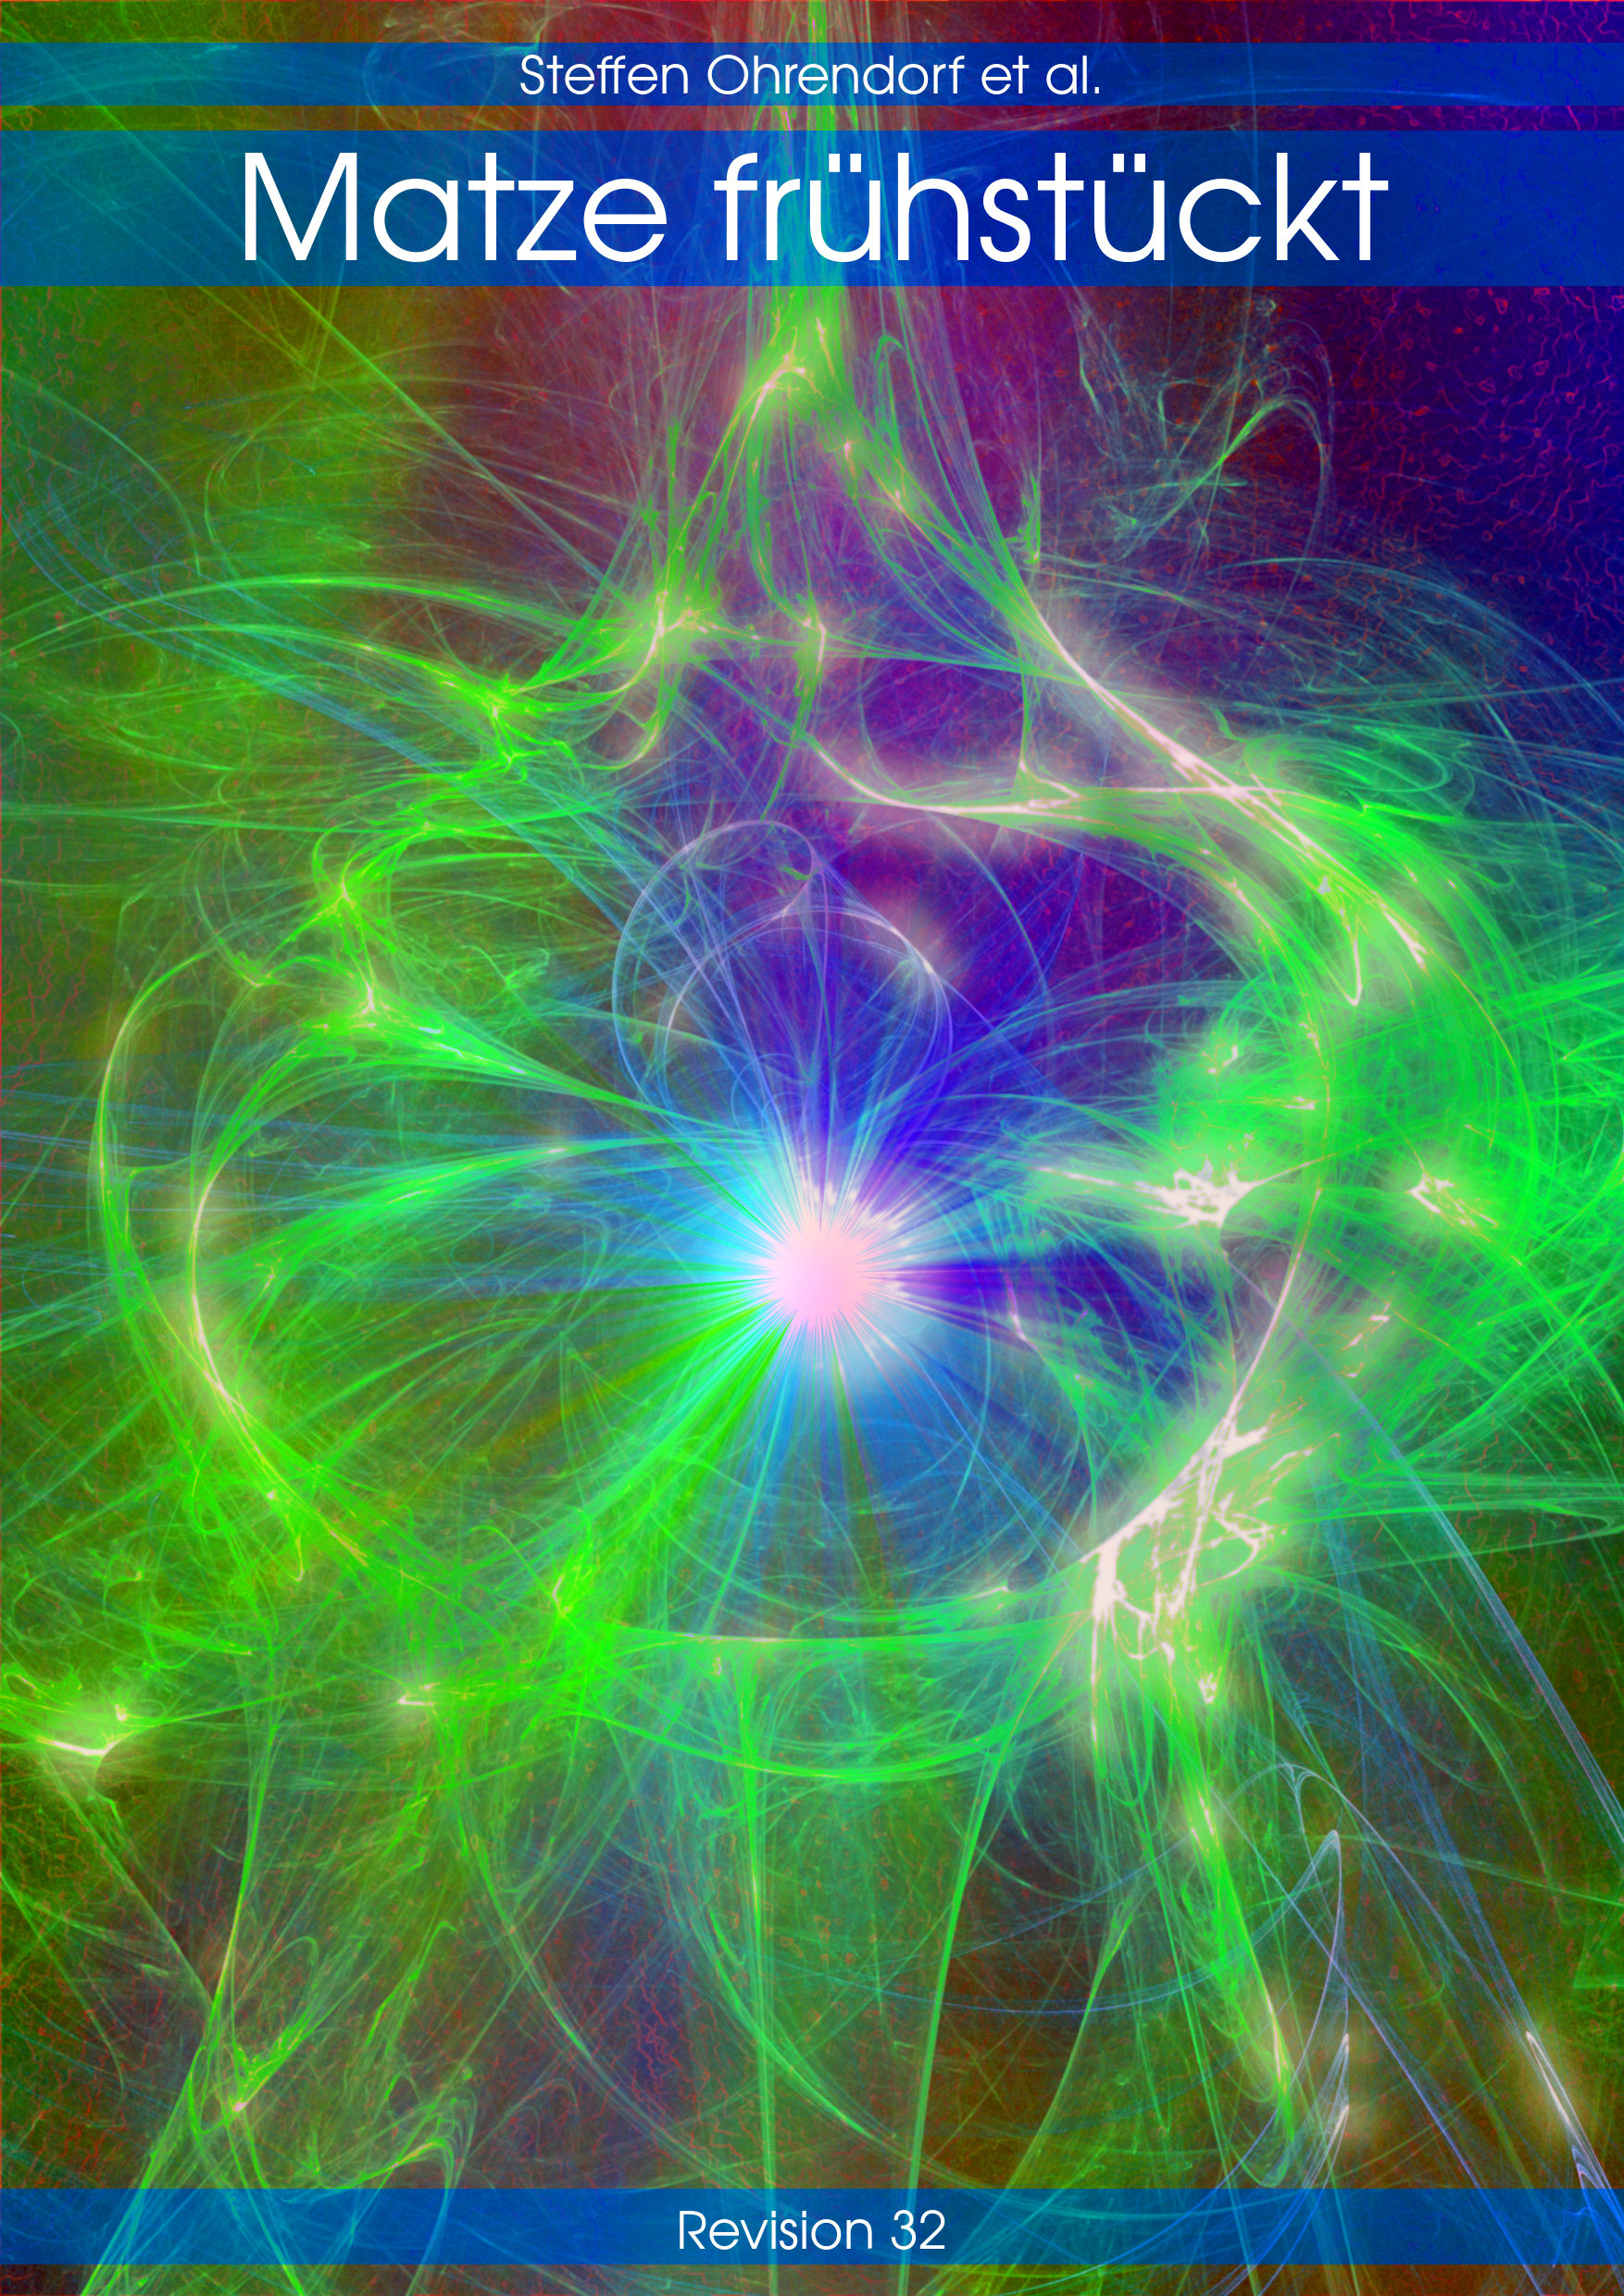
\includegraphics[height=210mm]{matse-cover-v3-3.jpg}}
\restoregeometry
\end{titlepage}


\clearpage\thispagestyle{empty}
\dictum[\url{http://german-bash.org/83851}]{Als Informatiker sollte man immer Linux zu Hause haben. Falls mal Besuch kommt.}

\vspace{1cm}
\dictum[Ian Sommerville, \cite{Sommerville}]{Bücher spiegeln naturgemäß die Meinungen und Vorurteile ihrer Autoren wider.
Es wird sich nicht vermeiden lassen, dass manche Leser mit meiner Einschätzung der Dinge und dem von mir ausgewählten Material nicht einverstanden sind.}

\vspace{4cm}
\begin{onehalfspace}
    \Large\sffamily
    Sollten Sie dieses Dokument käuflich erworben haben, ohne zu wissen, dass dies alles \textsl{kostenlos} im Internet verfügbar ist, sind Sie wohl Opfer eines Betrugs geworden.
\end{onehalfspace}

\vfill
\begin{flushright}
  Revision 32, \datemonthname\ \the\year
\end{flushright}

\clearpage

\thispagestyle{empty}
%
\ifthispageodd{}{\hbox{\ }\eject\thispagestyle{empty}}%
%
\newgeometry{top=0pt,left=0pt,right=0pt,inner=0pt,outer=0pt,marginparsep=0pt,marginparwidth=0pt}%
\noindent\kern-\parindent\vbox to 0pt{\kern-1em\includegraphics{uebersicht-page.pdf}}
\restoregeometry
\thispagestyle{empty}%
\clearpage

\hyphenation{ü-ber-tra-gen ü-ber-mitt-elt ü-ber-mitt-eln}


\chapter*{Urheberrecht}

\fancypagestyle{empty}{%
	\fancyhf{}
	\renewcommand{\headrulewidth}{0pt}
	\fancyhead[LE]{\lblob}
	\fancyhead[RO]{\rblob}
	\fancyfoot[C]{\ccbyncnd}
}
\thispagestyle{empty}
\hfil{\Huge\ccbyncnd}\hfil

\bigskip{}

Dieses Material steht unter der Creative-Commons-Lizenz Namensnennung -- Nicht kommerziell -- Keine Bearbeitungen 4.0 International.
Um eine Kopie dieser Lizenz zu sehen, besuchen Sie \url{http://creativecommons.org/licenses/by-nc-nd/4.0/deed.de}.

Dies bedeutet für Sie, dass Sie dieses Dokument unter folgenden Bedingungen gerne vervielfältigen dürfen:%
\footnote{Sei es nun eine einfache digitale Kopie, das Abtippen, das Binden als Buch, oder gar eine handschriftliche Kopie.}

\begin{itemize}
  \item Sie müssen meinen Namen nennen.
  \item Sie dürfen keine kommerzielle Verwertung dieses Dokuments durch\-führ\-en.
  \item Sie dürfen bei der Vervielfältigung inhaltlich nichts verändern.
\end{itemize}

Dies war nur eine grobe, nicht sehr genaue Zusammenfassung. Für Details
sehen Sie bitte unter dem oben angegebenen Link nach.

\clearpage\frontmatter
\tableofcontents{}
\mainmatter

\addchap{Vorwort}

Dieses Dokument ist \emph{nicht} als Skript zu verstehen und sollte nicht als alleinige Basis zum Lernen dienen.
Es ist als begleitendes Material gedacht, um eventuell das vorhandene Wiss\-en aufzufrischen.
Es ist eine sehr kompakte Zusammenfass\-ung der Pflichtkurse des Studienganges \emph{Scientific Programm\-ing} und enthält nur die Ergebnisse einiger Tausend Seiten Fachliteratur und vielen hundert Stunden Vorlesungen; daher erfordert dieses Dokument entweder gutes Begleitmaterial in Form von Vorlesungen oder Büchern, oder aber
den starken Willen und den großen Geist, sich die Beweise und Anwendungsgebiete der Formeln selbst herzuleiten.

Sie werden in diesem Buch übrigens kein Kapitel über Software Engineering finden, da dieses Thema weitaus komplexer ist, als dass es sich auf ein paar Seiten zusammenfassen ließe.
Eine bereits kompakte Zusammenfassung des Themas ist \enquote{Software Engineering} von Ian Sommerville (\cite{Sommerville}), und dieses Buch ist bereits über 800~Seiten dick.
Ich empfehle dringend, dieses Buch so früh wie möglich anzuschaffen, sofern Sie auch nur den Hauch mit Software-Entwicklung zu tun haben.

Als Ausgleich hierfür habe ich versucht, die anderen Themen etwas breiter zu fächern und etwas tiefer zu behandeln, weshalb Sie hier und da Dinge finden werden, die nicht in Ihren Vorlesungen behandelt werden.
Auf der anderen Seite kann ich nicht garantieren, dass Sie hier alles finden werden, was für Sie wichtig ist; sollten Sie also etwas vermissen, weisen Sie mich bitte darauf hin, so dass ich die Lücke füllen kann.

Wer beim Durchlesen oder Nachschlagen ein Thema nicht voll versteht, sollte \emph{auf jeden Fall} noch einmal einen Blick in die Literatur des entsprechenden Themas werfen.
Alternativ wäre die Wahl eines anderen Studiums sinnvoll.

\paragraph*{Ein kurzes Wort zu Revision 32}
Gegenüber der uralten Revision 31 hat sich so einiges getan.
Insbesondere habe ich das komplette Buch vollständig umgekrempelt und versucht, alles professioneller aussehen zu lassen.
Inhaltlich hat sich auch so einiges getan, unter anderem habe ich \emph{IT Systeme} in \emph{IT Grundlagen} eingearbeitet und den neuen Teil \emph{Algorithmen und Datenstrukturen} hinzugefügt.
Viele neue Abbildungen sind hinzugekommen, und die alten habe ich versucht zu verbessern; Struktogramme sind auf das Minimum reduziert und durch Pseudocode-Algorithmen ersetzt worden, da ich diese Darstellung für zielführender halte; sämtliche Formeln wurden überarbeitet, um konsistente Darstellung sicherzustellen, und insgesamt ist der Inhalt wesentlich kompakter geworden.
Zum Vergleich: Gegenüber Revision 31 wurde der Inhalt pro Seite um ca.~30--40\% erhöht, und die Seitenzahl nähert sich der Verdoppelung.
Obwohl ich erst die Hälfte des Weges gegangen bin (es fehlen immerhin noch die Teile Numerik, Rechnernetze und Datenbanken), bin ich stolz auf Revision 32, und hoffe, Sie finden Freude daran.

\Todo{Noch zu schreiben: Datenbanken}

\Todo{Noch zu schreiben: Rechnernetze}

\Todo{Noch zu schreiben: Analysis---Differenzialgleichungen}

\Todo{Zu überarbeiten: Analysis---Funktionen höherer Ordnung}

\addchap{Danksagung}

Ich möchte folgenden Personen für die Vorlesungen, Präsentationen, Notizen und Inspirationen danken:
\begin{itemize}
  \item Jens Hollmann (Analysis)
  \item Dr.~Alexander Voß (IT Grundlagen)
  \item Prof.~Dr.~Hans~Joachim Pflug (Java, sowie Algorithmen und Datenstrukturen)
  \item Benno Willemsen, M.\,Sc.\ (Lineare Algebra)
  \item Bastian Küppers, M.\,Sc.\ (IT-Systeme)
  \item Prof.~Dr.~Martin Reißel (Numerik)
  \item Prof.~Dr.~Volker Sander (Datenbanken)
  \item Prof.~Dr.~Horst Schäfer (Stochastik)
  \item Prof.~Dr.~rer.~nat.~Jörg Striegnitz (Rechnernetze)
  \item Prof.~Dr.~Andreas Terstegge (Software Engineering)
\end{itemize}

Weiterhin gilt mein Dank denjenigen, die mir unentgeltlich Material, Zeit und andere gute Sachen zur Verfügung gestellt haben:

\begin{itemize}
  \item Tim Böhmer für den Teil \enquote{Kombinatorik} (\cpageref{chap:Kombinatorik}).
  \item Frederic Klein für einen wichtigen Teil von \enquote{Lineare Gleichungssysteme} (\cpageref{sec:Lineare-Gleichungssysteme}).
  \item Mike Boddin für das Korrekturlesen von Revision 21.
  \item Einem Spender, der mich dazu angespornt hat, den Teil \enquote{Lineare Algebra} noch einmal zu überarbeiten und zu vervollständigen.
  \item Dipl.-Math.~Frank Schürmann für das intensive Korrigieren des Teils \enquote{Lineare Algebra} für Revision~32.
\ifincludeincomplete
  \item Anita Ludermann für die Vorlagen von \enquote{Datenbanken} (\cpageref{part:Datenbanken}).
\fi
\end{itemize}

\setpartpreamble{
  \dictum[Doctor Who]{All of Time and Space;\\
  everywhere and anywhere;\\
  every star that ever was.\\
  Where do you want to start?}
  \vspace{2em}\par%
  \dictum[Morpheus]{Ich kann Dir nur die Tür zeigen.
  Hindurchgehen musst Du alleine.}
}
\part{Mathematische Grundlagen}
\parttoc
% !TeX root = matze_fruehstueckt.tex
\chapter{\label{chap:mengenlehre}Mengenlehre}

\section{Definitionen}
\index{Cantor}\index{Menge|(}
\noindent
\begin{quotation}
  Eine Menge ist eine Zusammenfassung von bestimmten wohl unterschiedenen Objekten unserer Anschauung oder un\-ser\-es Denk\-ens---welche die Elemente der Menge genannt werden---zu einem Ganzen.
  \begin{flushright} (\noun{Cantor}) \end{flushright}
\end{quotation}

\begin{description}
  \item	[Explizite Aufzählung] \index{Menge!Aufzählung}\index{Aufzählung|see{Menge}}
	$M=\{ a,b,c,d,\ldots\} $
  \item	[Aufzählung nach Eigenschaft] \index{Menge!Eigenschaft}
	$P=\{ x\mid \hbox{$x$ ist Primzahl}\} $
  \item [Leere Menge] \index{Menge!leer}
	$\emptyset$ oder $\{\}$.
	Achtung: $\{\emptyset\}=\{\{\}\}$ ist eine Menge, die eine leere Menge enthält. Es gilt $\forall M:\emptyset\in M$.
  \item [(Echte) Teilmenge] \index{Menge!Teilmenge}
	$A$ ist (echte) Teilmenge von $B$: $A\subset B:=A\neq B\land\forall a\in A:a\in B$.
  \item [Unechte Teilmenge]
	$A$ ist (unechte) Teilmenge von $B$: $A\subseteq B:=\forall a\in A:a\in B$.
    [Da $\subset$ oftmals die Bedeutung von $\subseteq$ hat, kann für echte Teilmengen auch $\subsetneq$ verwendet werden.]
  \item [Durchschnitt (Schnittmenge)] \index{Menge!Durchschnitt}\index{Menge!Schnittmenge}
	$A\cap B:=\{ x\mid x\in A\land x\in B\} $
  \item [Vereinigung] \index{Menge!Vereinigung}
	$A\cup B:=\{ x\mid x\in A\lor x\in B\} $
  \item [Differenzmenge] \index{Menge!Differenzmenge}
	$A\setminus B:=\{ x\mid x\in A\land x\notin B\} $
\end{description}

\begin{figure}[htb]
\caption{\noun{Venn}-Diagramme}

\includegraphics{venn-1.pdf}
\hfill{}
\includegraphics{venn-2.pdf}
\hfill{}
\includegraphics{venn-3.pdf}
\end{figure}

\index{Menge|)}

\section{Rechenregeln}

Prioritäten, absteigend sortiert: Klammern, Komplement, Durchschnitt,
Vereinigung.
\begin{description}
  \item [Kommutativgesetz] \index{Menge!Kommutativgesetz}
	$A\cap B=B\cap A$,
	$A\cup B=B\cup A$
  \item [Assoziativgesetz] \index{Menge!Assoziativgesetz}
	$(A\cap B)\cap C=A\cap(B\cap C)$,
	$(A\cup B)\cup C=A\cup(B\cup C)$
  \item [Distributivgesetz] \index{Menge!Distributivgesetz}
	$A\cap(B\cup C)=(A\cap B)\cup(A\cap C)$,
	$A\cup(B\cap C)=(A\cup B)\cap(A\cup C)$
  \item [Transitivgesetz] \index{Menge!Transitivgesetz}
	$A\subset B\land B\subset C\Rightarrow A\subset C$
  \item [Komplement] \index{Menge!Komplement}
	$\bar{\mathbb{R}}=\emptyset$,
	$\bar{\emptyset}=\mathbb{R}$,
	$\bar{\bar{A}}=A$
  \item [Mächtigkeit/Kardinalität] \index{Menge!Mächtigkeit}\index{Menge!Kardinalität}
	Anzahl der eindeutigen Elemente: $\lvert A \rvert$, manchmal auch $\#A$.
  \item [Potenzmenge] \index{Menge!Potenzmenge}
	Menge aller Teilmengen einer Menge: $\mathcal P(A)$. Es ist $\lvert \mathcal P(A) \rvert = 2 \uparrow \lvert A \rvert$.
  \item [Kreuzprodukt] \index{Menge!Kreuzprodukt}\index{Kreuzprodukt|see{Menge}}\index{Menge!Produktmenge}\index{Menge!kartesisches Produkt}\index{kartesisches Produkt|see{Menge}}
	$A\times B:=\{ (a,b)\mid a\in A\land b\in B\} $
\end{description}

\subsection{\protect\noun{De Morgan}sche Regeln}

\index{de Morgan}
\index{Menge!de Morgan}
\begin{align*}
  A\setminus(B\cap C)  & =(A\setminus B)\cup(A\setminus C)\\
  A\setminus(B\cup C)  & =(A\setminus B)\cap(A\setminus C)\\
  \overline{(A\cup B)} & =\bar{A}\cap\bar{B}\\
  \overline{(A\cap B)} & =\bar{A}\cup\bar{B}
\end{align*}



\section{Relationen}

\index{Relation|see{Menge}}
\index{Menge!Relation}
Eine Relation $R$ auf einer Menge $A$ ist eine (unechte) Teilmenge von $A\times A$.

\begin{description}
  \item [Reflexivität] \index{Reflexivität|see{Äquivalenzrelation}}\index{Menge!reflexiv}
	$\forall a\in A:(a,a)\in R$
  \item [Symmetrie] \index{Symmetrie|see{Menge}}\index{Menge!symmetrisch}
	$\forall a,b\in A:(a,b)\in R \iff (b,a)\in R$
  \item [Transitivität] \index{Transitivität|see{Menge}}\index{Menge!transitiv}
	$\forall a,b,c\in A:(a,b)\in R\land(b,c)\in R\Rightarrow(a,c)\in R$
  \item [Äquivalenzrelation] Eine \index{Äquivalenzrelation|see{Menge}}\index{Menge!Äquivalenzrelation}
	Äquivalenzrelation $\sim$ auf einer Menge $M$ muss reflexiv, symmetrisch und transitiv (\emph{rst}) sein.
	Es gilt dann: $(a,b)\in R \iff a\sim b$.
\end{description}


\subsection{Totale und partielle Ordnung}
\index{totale Ordnung}
\index{Ordnung!total}
Eine totale Ordnung auf einer Menge $M$ ist definiert, wenn $\forall x,y,z \in M$ gilt:
\noindent\begin{center}
\begin{tabular}{rl}
	                                        $x \leq x$ & Reflexivität  \\
	     $x \leq y \land y \leq x\; \Rightarrow\; x=y$ & Antisymmetrie \\
	$x \leq y \land y \leq z\; \Rightarrow\; x \leq z$ & Transitivität \\
	                          $x \leq y \lor y \leq x$ & Totalität
\end{tabular}
\end{center}

\index{partielle Ordnung}
\index{topologische Ordnung}
\index{Ordnung!partiell}
\index{Ordnung!topologisch}
Vernachlässigt man die Forderung nach Totalität (d.\,h., dass nicht jedes Element mit jedem Element vergleichbar ist), so erhält man die Definition einer \emph{partiellen} bzw.~\emph{topologischen} Ordnung.
Z.\,B.~ist das Inhaltsverzeichnis dieses Buches partiell, aber nicht total, nach \enquote{Voraussetzungen} geordnet:
\noindent\begin{quote}
    \noindent Grundlagen $\preceq$ Kurvendiskussion $\preceq$ Vektoranalysis
    \par\hfill $\Rightarrow$ Grundlagen $\preceq$ Vektoranalysis

    \noindent Grundlagen $\preceq$ Matrizen $\preceq$ Lineare Abbildungen
    \par\hfill $\Rightarrow$ Grundlagen $\preceq$ Lineare Abbildungen
    
    \noindent Aber: Matrizen und Vektoranalysis sind nicht vergleichbar.
\end{quote}
[Für partielle Ordnungen werden die Begriffe \enquote{Vorgänger} und \enquote{Nachfolger} statt \enquote{kleiner} bzw.~\enquote{größer} verwendet, sowie gekrümmte Operatoren wie $\prec$, $\preceq$ oder~$\asymp$.]


\section{Gruppe}

Eine nicht-leere Menge $M$, auf der eine Verknüpfung~$\circ$ definiert
ist, heißt \index{Gruppe}Gruppe, wenn für $\forall x,y,z\in M$
gilt:
\begin{description}
  \item [Abgeschlossenheit] \index{Abgeschlossenheit|see{Gruppe}}\index{Gruppe!abgeschlossen}
	$x\circ y\in M$
  \item [Assoziativität] \index{Assoziativität|see{Gruppe}}\index{Gruppe!assoziativ}
	$(x\circ y)\circ z=x\circ(y\circ z)$
  \item [Neutralelement] \index{Neutralelement|see{Gruppe}}\index{Gruppe!Neutralelement}
	Es existiert \emph{genau ein} Element $n\in M$, für das gilt: $x\circ n=n\circ x=x$
  \item [Inverses Element] \index{inverses Element|see{Gruppe}}\index{Gruppe!inverses Element}
	Zu jedem $x\in M$ existiert ein $x^{-1}\in M$, für das
	$x\circ x^{-1}=x^{-1}\circ x=n$ gilt.
	[Das inverse Element $x^{-1}$ ist nicht mit dem Kehrwert zu verwechseln.]
\end{description}

Mit dieser zusätzlichen Bedingung heißt die Gruppe kommutativ oder \noun{Abel}sch:
\begin{description}
  \item [Kommutativ] \index{Kommutativ|see{Gruppe}}\index{Abelsch|see{Gruppe}}\index{Gruppe!kommutativ}\index{Gruppe!Abelsch}
	$x\circ y=y\circ x$
\end{description}

\section{Ring}

Eine nicht-leere Menge $M$ heißt \index{Ring}Ring, wenn auf ihr zwei Verknüpfungen $\oplus$ und $\odot$ mit folgenden Eigenschaften definiert sind:

\begin{enumerate}
  \item $M$ ist eine kommutative Gruppe bezüglich $\oplus$.
  \item Ohne das Neutralelement bzgl.~$\oplus$ erfüllt der Rest von $M$ alle Axiome einer Gruppe bezüglich $\odot$, jedoch \emph{nicht} das Axiom des inversen Elements.
  \item Es gelten die Distributivgesetze ($\forall x,y,z\in M$):
	\begin{align*}
	  (x\oplus y)\odot z & =(x\odot z)\oplus(y\odot z)\\
	  x\odot(y\oplus z) & =(x\odot y)\oplus(x\odot z)
	\end{align*}
\end{enumerate}

[Das neutrale Element bezüglich der \enquote{Addition} $\oplus$ wird oft mit~0 bezeichnet, das neutrale Element bezüglich der \enquote{Multiplikation} $\odot$ oft als~1.]


\section{Körper}

Eine nicht-leere Menge $M$ heißt \index{Körper}Körper, wenn sie die Eigenschaften des Ringes erfüllt und zusätzlich ein inverses Element bezüglich $\odot$ besitzt.


\section{Abbildungen}

\index{Abbildung|(}
\begin{description}
  \item [Funktion/Abbildung] \index{Funktion}
	$f:A\rightarrow B$ oder $f:A\ni a\rightarrow f(a)\in B$
  \item [Definitionsbereich] \index{Definitionsbereich}
	Das $A$ bei $f:A\rightarrow B$.
  \item [Zielmenge] \index{Zielmenge}
	Das $B$ bei $f:A\rightarrow B$.
  \item [Bildmenge] \index{Bildmenge}
	$f(A)\subseteq B$, auch: Wertemenge\slash{}Bild von $A$ bzgl.~$f$.
  \item [Urbild] \index{Urbild}
	$f^{-1}(b):=\{a\in A\mid f(a)=b\}\subseteq A$, Urbild von $b\in B$.
  \item [Injektivität] \index{Abbildung!injektiv}\index{Injektivität}
	$f(u)=f(v) \implies u=v$.
  \item [Surjektivität] \index{Abbildung!surjektiv}\index{Surjektivität}
	$f(A)=B$.
  \item [Bijektivität] \index{Abbildung!bijektiv}\index{Bijektivität}
	Injektiv und surjektiv.
\end{description}

\subsection{Homomorphismus}

\index{Abbildung!linear}\index{Abbildung!Homomorphismus}\index{Homomorphismus}
Seien $A$ und $B$ Vektorräume über einem Körper $K$\@.
Eine Abbildung $f : A\rightarrow B$ heißt \emph{Homomorphismus} bzw.~\emph{lineare Abbildung}, falls gilt:
\begin{description}
  \item [Additivität] $\forall x,y\in A : f(x+y)=f(x)+f(y)$
  \item [Homogenität] $\forall x\in A\;\forall\lambda\in K : f(\lambda\cdot x)=\lambda\cdot f(x)$
\end{description}

Die Menge der linearen Abbildungen von $A$ nach $B$ wird mit $\hom(A,B)$ bezeichnet.
\begin{description}
  \item [Kern] \index{Abbildung!Nullraum}\index{Nullraum}\index{Abbildung!Kern}\index{Kern}
	von $f$ bzw.~\emph{Nullraum} von $f$ ist definiert als $\ker(f) := \{ x \in A \mid f(x)=0 \}$.
	Enthält entweder genau ein Element (die 0) oder unendlich viele.
  \item [Regulär] \index{regulär}\index{Abbildung!regulär}
	$\ker(f)=\{0\}$
  \item [Singulär] \index{singulär}\index{Abbildung!singulär}
	$\lvert\ker(f)\rvert = \infty$
  \item [Isomorphismus] \index{Isomorphismus}\index{Abbildung!isomorph}
	ist ein bijektiver Homomorphismus.
\end{description}

\index{Abbildung|)}


\section{Modulo-Arithmetik}

\index{Modulo-Arithmetik}\index{Restklasse}\index{Kongruenz|see{Restklasse}}
Zwei Zahlen $a,b\in\mathbb{Z}$ heißen zu einer festen Zahl $m\in\mathbb{N}\setminus\{0\}$ kongruent modulo $m$, wenn gilt:
\[ a\equiv b \pmod m \quad \iff \quad \lvert a-b \rvert = n\cdot m,\,n\in\mathbb{N} \]

Das heißt, dass die Differenz beider Zahlen $a$ und $b$ durch $m$ teilbar ist.

Weiter gelten:
\begin{align*}
  (x +     y) \bmod p & =((x\bmod p)+(y\bmod p)) \bmod p \\
  (x \cdot y) \bmod p & =((x\bmod p)\cdot(y\bmod p))\bmod p\\
  x^n \bmod p         & = (x\bmod p)^n \bmod p
\end{align*}



\chapter{\label{chap:Kombinatorik}Kombinatorik}

\index{Kombinatorik|(}
Die Kombinatorik beschreibt eine Auswahl von $k$ Objekten aus $n$ Elementen, welche in einer Ergebnismenge\index{Ergebnismenge} zusammengefasst werden.
Gesucht ist dann die Mächtigkeit\index{Mächtigkeit} $a$ der Ergebnismenge.

\begin{description}
  \item [Permutation] \index{Permutation}
	Berücksichtigung der Reihenfolge
  \item [Kombination] \index{Kombination}
	Ignorieren der Reihenfolge
\end{description}

\noindent\begin{center}
\begin{tabular}{rcc}
              & \bfseries mit Wdh.
              & \bfseries ohne Wdh. \\
  \bfseries Perm.
              & $\left|\mathrm{PER}^{\mathrm{MW}}(n,k)\right| = n^k$
              & $\left|\mathrm{PER}^{\mathrm{OW}}(n,k)\right| = \vecc(n;k) k!$ \\[1.6667em]
  \bfseries Komb.
              & $\left|\mathrm{KOM}^{\mathrm{MW}}(n,k)\right| = \vecc(n+k-1;k)$
              & $\left|\mathrm{KOM}^{\mathrm{OW}}(n,k)\right| = \vecc(n;k)$
\end{tabular}

\vspace{0.66667em}
\emph{Betragsstriche beachten! Die Funktionen geben die Kombinationen bzw.~Permutationen zurück.}
\end{center}

\begin{description}
  \item [Teilchen-/Fächermodell] \index{Teilchenmodell}\index{Fächermodell}\index{Grundmenge}
	Grundmenge: Fächer, Auswahl: Besetzung der Fäch\-er mit Teilchen.

	Mächtigkeit der Grundmenge ist Anzahl der Fächer, Experiment erfolgt durch Verteilen der Teilchen in die Fächer.

  \item [Urnenmodell] \index{Urnenmodell}
	Grundmenge: Kugeln in Urne, Auswahl: Ziehung der Kugeln.

	Mächtigkeit der Grundmenge ist Anzahl der Kugeln, Experiment besteht aus Ziehung der Kugeln.
\end{description}

\index{Kombinatorik|)}


\chapter{Komplexe Zahlen}
\begin{description}
  \item [Definition] \index{Komplexe Zahl}
	$z = x+iy = r\cdot e^{i\varphi} = r\cdot (\cos(\varphi)+i\sin(\varphi))$
  \item [Realteil] $\Re(z) = \mathrm{Re}(z) = x$
  \item [Imaginärteil] $\Im(z) = \mathrm{Im}(z) = y$
  \item [Konjugiert komplex] \index{Komplexe Zahl!konjugiert komplex}\index{konjugiert komplex|see{Komplexe Zahl}}
	$\bar{z} = x-iy$
  \item [Betrag] \index{Komplexe Zahl!Betrag}\index{Betrag|see{Komplexe Zahl}}
	$\lvert z \rvert = \sqrt{x^2+y^2} = \sqrt{z\cdot\bar{z}}$
  \item [Potenzen] \index{Komplexe Zahl!Potenzen}
	$z^n = r^n \cdot \exp(n\cdot i\varphi)$
  \item [Wurzeln] \index{Komplexe Zahl!Wurzeln}
	$\sqrt[n]{z} = \sqrt[n]{r} \cdot \exp \bigl( (i\varphi+2k\pi i)/n\bigr), \quad 0 \leq k < n$
\end{description}

\section{Polarkoordinaten}

\index{Komplexe Zahl!Polarkoordinaten}\index{Polarkoordinaten|see{Komplexe Zahl}}
\[
  \varphi=\begin{cases}
     \arccos(\mathrm{Re}(c) / \lvert c \rvert) & \hbox{für $\mathrm{Im}(c) \geq 0$}\\
    -\arccos(\mathrm{Re}(c) / \lvert c \rvert) & \hbox{für $\mathrm{Im}(c) < 0$}
  \end{cases}
\]


\chapter{Sonstiges}

\section{\label{sec:intervalle}Intervalle}

\begin{align*}
  \left[a;b\right]   & =\{ x\mid a\leq x\leq b\} =a\leq x\leq b\\
  \left[a;b\right[   & =\{ x\mid a\leq x<b\}     =a\leq x<b\\
  \left]a;b\right]   & =\{ x\mid a<x\leq b\}     =a<x\leq b\\
  \left]a;b\right[   & =\{ x\mid a<x<b\}         =a<x<b
\end{align*}
[Für $a=-\infty$ bzw.~$b=\infty$ sind jeweils offene Grenzen zu benutzen.]


\section{\label{hornerschema}\noun{Horner}schema}
\index{Hornerschema}
Das \noun{Horner}schma kann zur Abspaltung von Linearfaktoren in Polynomen verwendet werden.
Sei $f(x)=\sum_{0 \leq i \leq n} a_i x^i$ ein Polynom $n$-ten Grades, und $x-x_0$ ein abzuspaltender Linearfaktor, so lässt sich $f(x)$ umschreiben als $f(x)=r+(x-x_0)\cdot\sum_{0 \leq i < n} b_i x^i$:

\noindent\begin{center}
\begin{tabular}{l|l|l|l|l}
	$a_n$         & $a_{n-1}$              & $a_{n-2}$              & $\cdots$ & $a_0$                \\ \hline
	$x_0=\ldots$  & $+(b_{n-1} \cdot x_0)$ & $+(b_{n-2} \cdot x_0)$ & $\cdots$ & $+(b_{0} \cdot x_0)$ \\
	$b_{n-1}=a_n$ & $=b_{n-2}$             & $=b_{n-3}$             & $\cdots$ & $=r$
\end{tabular}
\end{center}

\emph{Achtung:} Fehlende $a_i$ sind mit~$0$ in die Tabelle einzutragen!

[Wenn $r=0$ ist, ist $x_0$ eine Nullstelle von $f(x)$.]

Beispiel für $x_0=2$ und $f(x)=x^5 - 4x^4 + 4x^3 + 3x^2 - 8x + 4$:
\noindent\begin{center}
\begin{tabular}{r|r|r|r|r|r}
	$1$     & $-4$ & $4$  & $3$ & $-8$ & $4$  \\ \hline
	$x_0=2$ & $2$  & $-4$ & $0$ & $6$  & $-4$ \\
	$1$     & $-2$ & $0$  & $3$ & $-2$ & $0$
\end{tabular}
\end{center}
Damit: $f(x) = (x^4 - 2x^3 + 0x^2 + 3x - 2)\cdot(x-2) + 0$, also ist $2$ eine Nullstelle von $f(x)$.


\section{Regel von \noun{L'Hospital}}
\index{L'Hospital}
\index{Regel!von L'Hospital}
Wenn eine Funktion $u(x)=f(x)/g(x)$ als Ergebnis $0/0$ oder $\pm \infty/\infty$ liefert, ist $u(x)=f'(x)/g'(x)$.
[\emph{Achtung:} Die Fälle $0/\infty$ und $\infty/0$ sind hiervon \emph{nicht} betroffen.]



\chapter[Vollständige Induktion]{Beweis durch vollständige Induktion}

\CheckedBox{} Beispiel vorhanden auf \cpageref{sec:bsp-Vollständige-Induktion}.
\begin{description}
  \item [Induktionsanfang (IA)] \index{Induktion!vollständige --}
	Beweise, dass eine Aussage $f(n)=g(n)$ für ein ge\-wählt\-es $n_{0}$ gilt (i.\,d.\,R.~für $n_{0}=1$).
  \item [Induktionsvoraussetzung (IV)]
	Gleichsetzen der rekursiven Formel und der expliziten Formel, also $f(n)=g(n)$ explizit aufschreiben.
  \item [Induktionsbehauptung (IB)]
	Satz: \enquote{Wenn $f(n)=g(n)$ für ein beliebiges aber festes $n$ gilt, so gilt die Aussage auch für $n+1$.}
  \item [Induktionsschluss (IS)]
	Überprüfen, ob $f(n+1)=g(n+1)$ unter Verwendung der IV stets eine wahre Aussage ergibt, d.\,h., eine Seite der Aussage muss mit Hilfe der IV in die andere Seite umgeformt werden.
	Beim Einsetzen der IV sollte über dem Gleichheitszeichen \enquote{IV} stehen.
	Schlusssatz: \enquote{Damit ist die IV bewiesen.}
\end{description}


\chapter{\noun{Bool}sche Algebra und Aussagenlogik}

Beachte Ähnlichkeiten zur Mengenlehre, \cpageref{chap:mengenlehre}.

\begin{description}
    \item[Aussage] $A$, $B$, \ldots bzw.~$a(x)$, $b(x)$\ldots
    \item[Tautologie] $\models A$ heißt, dass $A$ unabhängig seiner abhängigen Variablen wahr ist.
    \item[Negation] $\neg A$ oder $\overline{A}$
    \item[Bikonditional] $A \leftrightarrow B$; $A$ genau dann, wenn $B$. Falls $A \leftrightarrow B$ eine Tautologie ist,
                         schreibt man $A \Leftrightarrow B$.
    \item[Konjunktion] $A \land B$; $\neg(A \land B) \leftrightarrow (\neg A \lor \neg B)$
    \item[Disjunktion] $A \lor B$; $\neg(A \lor B) \leftrightarrow (\neg A \land \neg B)$
    \item[Implikation] $(A \rightarrow B) := (\neg A \lor B)$, $A \vdash B$, $B \subset A$, auch
                       \enquote{Konditional} oder \enquote{Subjunktion} genannt; $A$ ist eine hinreichende
                       Bedingung für $B$, $B$ ist eine notwendige Bedingung für $A$. Falls $A \rightarrow B$ eine Tautologie
                       ist, schreibt man $A \Rightarrow B$ oder $A \models B$.
    \item[Kontravalenz] $\neg(A \leftrightarrow B) \leftrightarrow (A \oplus B)$, ausschließendes Oder.
\end{description}

[\enquote{Doppelstrich-Operatoren} wie $\models$, $\Rightarrow$ oder $\Leftrightarrow$ drücken damit aus, dass eine gegebene
Aussage unabhängig ihrer abhängigen Variablen wahr ist; die analogen Operatoren $\vdash$, $\rightarrow$ und $\leftrightarrow$ sagen lediglich aus, dass die entsprechende Aussage syntaktisch hergeleitet werden kann, d.\,h.~$A \rightarrow \neg A$ ist korrekt, jedoch $A \Rightarrow \neg A$ nicht.]


\begin{table}[htb]
    \centering\begin{tabular}{rcl}
    	             $(A \lor A)$ &   $\rightarrow$   & $A$                            \\
    	                      $B$ &   $\rightarrow$   & $(A \lor B)$                   \\
    	             $(A \lor B)$ &   $\rightarrow$   & $(B \lor A)$                   \\
    	    $(A \lor (B \lor C))$ &   $\rightarrow$   & $(B \lor (A \lor C))$          \\
    	      $(A \rightarrow B)$ &   $\rightarrow$   & $((C \lor A) \lor (C \lor B))$ \\
    	$(\neg(A \rightarrow B))$ & $\leftrightarrow$ & $(\neg B \rightarrow \neg A)$
    \end{tabular}
    \caption{Axiome der Aussagenlogik}
\end{table}


\setpartpreamble{
  \dictum[\noun{René Descartes}]{Denn es ist nicht genug, einen guten Kopf zu haben; die Hauptsache ist, ihn richtig anzuwenden.}
}
\part{Lineare Algebra}
\parttoc
% !TeX root = matze_fruehstueckt.tex
\chapter{Vektoren, Vektorräume}

\index{Vektor|(}


\section{Wichtige Begriffe}
\begin{description}
  \item [{Vektor}]
	Gerichtete Strecke ohne Position.
  \item [{Gebundener~Vektor}] \index{Vektor!gebunden}
	Vektor mit Position, zwischen zwei Punkten: $\overrightarrow{PQ}$.
  \item [{Ortsvektor}] \index{Ortsvektor}\index{Vektor!Orts--}
	Gebundener Vektor mit Position im Ursprung.
  \item [{Parallelität}] \index{Vektor!parallel}
	$\exists\alpha : \vec{a} = \alpha\vec{b} \iff \vec{a} \| \vec{b}$
	(gleiche Richtung: $\alpha>0$, gegensätzliche Richtung: $\alpha<0$).
  \item [{Orthogonalität}] \index{Vektor!orthogonal}
	$\langle \vec{a},\vec{b} \rangle = 0
	  \quad\iff\quad
	  \vec{a}\bot\vec{b}
	  \quad\iff\quad
	  \lVert \vec{a}+\vec{b} \rVert^2 = \lVert\vec{a}\rVert^2 + \lVert\vec{b}\rVert^2$
\end{description}

\subsection{Vektorraum}

\index{Vektorraum}
Sei $K$ ein beliebiger Körper und $V$ eine nicht-leere Menge.
$V$ heißt Vektorraum, wenn für $\forall x,y\in V$ und $\forall\lambda,\mu\in K$ gilt:

\begin{itemize}
  \item Folgende Abbildungen sind definiert:
    \[ x       \oplus y : \quad V\times V \to V, \qquad(x,y)      \mapsto x\oplus y \]
    \[ \lambda \odot  x : \quad K\times V \to V, \qquad(\lambda,x)\mapsto\lambda\odot x \]
  \item $V$ ist eine kommutative Gruppe bezüglich $\oplus$.
  \item $\lambda\odot(\mu\odot x)=(\lambda\cdot\mu)\odot x$.
  \item $1\odot x=x$ (hier ist $1$ das Neutralelement bzgl.~der Multiplikation aus $K$).
  \item $\lambda\odot(x\oplus y)=(\lambda\odot x)\oplus(\lambda\odot y)$.
  \item $(\lambda+\mu)\odot x=(\lambda\odot x)\oplus(\mu\odot x)$.
\end{itemize}

Dabei nennt man die $x$, $y$ \emph{Vektoren} und die $\lambda$, $\mu$ \index{Skalar}\emph{Skalare}.
\begin{description}
  \item [Linearkombination]
        $\sum_{1 \leq i \leq n} \lambda_i \vec v_i$ heißt Linearkombination von $\vec v_1, \ldots, \vec v_n$.
  \item [linear unabhängig]
        $n$ Vektoren $\vec v_1, \ldots, \vec v_n$sind genau dann linear unabhängig, wenn $\sum_i \lambda_i \vec v_i = 0 \Rightarrow \lambda_1,\ldots,\lambda_n = 0$ ist.
  \item [Lineare Hülle]
	Die Menge aller Linearkombinationen
	\[ L=\biggl\{ \sum_i \lambda_i \vec v_i \biggm| \lambda_i \in K\biggr\} \subseteq V \]
	heißt lineare Hülle von $\vec{v}_{1},\ldots,\vec{v}_{n}$.
  \item [Erzeugendensystem]
	Gilt $L(\vec v_1,\ldots,\vec v_n)=V$, so bilden die Vektoren ein Erzeugendensystem.
  \item [Basis]
	Auch: \emph{minimales Erzeugendensystem}.
	Ist ein Erzeugendensystem, bei dem die Vektoren linear unabhängig sind.
	Daher hat eine Basis für einen Vektorraum $V$ mit $\dim(V)=n$ genau $n$ Basisvektoren.
  \item [Dimension]
	Hat ein Vektorraum $V$ eine Basis $\{ \vec v_1,\ldots,\vec v_n\}$, so ist $\dim(V)=n$.
\end{description}

\subsubsection{Untervektorraum}

\index{Unterraum}\index{Vektorraum!Unter-}\index{Untervektorraum}
Eine nicht-leere Teilmenge $U$ eines Vektorraums $V$ über einem Körper $K$ ist ein Untervektorraum, wenn gilt:
\[ \forall x,y\in U,\; \forall\lambda\in K\ :\ x+y\in U\land\lambda x\in U \]

\subsection{Skalarprodukt}
\index{Skalarprodukt}\index{Vektorraum!Skalarprodukt}
$V$ sei bel.~Vektorraum über einem Körper $K\in\{\mathbb{R},\mathbb{C}\}$ und $a,\, b,\, c\in V$ sowie $\lambda\in K$, dann heißt $\langle \ast,\ast \rangle : V\times V\to K$ Skalarprodukt falls gilt:
\begin{description}
  \item [{SP1}]
	$\langle a,b\rangle =\overline{\langle b,a\rangle}$
	[Gilt wegen fehlendem Imaginärteil auch für $K\ne\mathbb{C}$.]
  \item [{SP2}]
	$\langle a,b+c\rangle =\langle a,b\rangle +\langle a,c\rangle $
	und $\langle a+b,c\rangle =\langle a,c\rangle +\langle b,c\rangle $
  \item [{SP3}]
	$\langle \lambda a,b\rangle =\lambda\langle a,b\rangle =\langle a,\bar{\lambda}b\rangle $
	[Gilt wegen fehlendem Imaginärteil auch für $K\ne\mathbb{C}$.]
  \item [{SP4}]
	$\langle a,a \rangle = 0 \iff a=0$
	und $\langle a,a \rangle > 0 \iff a\ne0$
  \item [{Standardskalarprodukt}] $\langle \vec{a},\vec{b}\rangle :=\sum_{i} a_i b_i$
\end{description}

\subsection{\label{sub:Vektornorm}Norm}

\index{Norm}\index{Vektor!Norm}
Sei $V$ ein Vektorraum über $K \in \{\mathbb R, \mathbb C\}$ sowie $a,b \in V$ und $\lambda \in K$, dann heißt $\lVert*\rVert : V \to \mathbb R$ Norm falls $\forall a,b \in V$ und $\forall\lambda \in K$ gilt:
\begin{description}
  \item [{N1}]
	$\lVert a\rVert\geq0$
  \item [{N2}]
	$\lVert a\rVert=0 \iff a=0$
  \item [{N3}]
	$\lVert \lambda a \rVert  =  \lvert \lambda \rvert \, \lVert a \rVert$
  \item [{N4}]
	$\lVert a+b\rVert\leq\lVert a\rVert+\lVert b\rVert$ (Dreiecksungleichung)
  \item [{Standardnorm}] \index{Vektor!Betrag}\index{Vektor!Euklidische Norm}\index{Vektor!Zweiernorm}\index{Betrag}\index{Norm!Betrag}\index{Norm!Zweier--}\index{Norm!euklidische}\index{Vektor!Standardnorm}\index{Norm!Standard--}
	$\lVert a\rVert=\sqrt{\langle a,a\rangle }$ (auch \emph{euklidische Norm}, \emph{Zweiernorm} oder \emph{Betrag})
  \item [{Betragssummennorm}] \index{Vektor!Einernorm}\index{Vektor!Betragssummennorm}\index{Norm!Einer--}\index{Norm!Betragssummen--}
	$\lVert a\rVert_1=\sum_{i}\lvert a_i \rvert$ (auch \emph{Einernorm})
  \item [{Maximumnorm}] \index{Vektor!Maximumnorm}\index{Norm!Maximum--}
	$\lVert a\rVert_{\infty} = \max\bigl\{\lvert a_i \rvert \bigr\}$
  \item [{Einheitsvektor}] \index{Vektor!Einheits--}\index{Einheitsvektor}
	$\lVert a\rVert=1$
  \item [{Kanonischer~Einheitsvektor}] \index{Vektor!kanonischer Einheits--}\index{Einheitsvektor!kanonisch}
	$\lVert a\rVert=1\land\exists! a_i : a_i=1$
\end{description}
\index{Metrik}\index{metrischer Raum}\index{Raum!Metrik}\index{Isometrie}
\label{metrischer-raum}
[Die Norm stellt einen Spezialfall einer Metrik $d(x,y)=\lVert x-y \rVert$ dar; eine Abbildung $d : M \times M \to \mathbb R$ auf \emph{beliebigen} Mengen $M$ heißt Metrik, wenn sie (i)~$d(x,y)\geq0$, (ii)~$d(x,y)=0 \iff x=y$, (iii)~$d(x,y)=d(y,x)$ und (iv)~$d(x,y) \leq d(x,z)+d(y,z)$ erfüllt.
Ist $d$ auf einer Menge $M$ definiert, so heißt $(M,d)$ metrischer Raum; eine auf diesem Raum definierte Abbildung $f : M \to M$ heißt Isometrie.]

\subsection{\label{sub:Errechnung-von-Normalen}Errechnung von Normalen}

Sei $\vec{v}$ ein Vektor mit $n$ Komponenten, so lassen sich dazu $n-1$ senkrechte linear unabhängige Vektoren nach folgendem Prinzip errechnen:
\begin{enumerate}
  \item Auswahl einer Komponente $n_i \neq 0$.
  \item Vertauschung von $n_i$ mit einer anderen Komponente $n_j$ ($i\neq j$) und Setzung der restlichen Komponenten auf~$0$.
  \item Negation einer der gewählten gebliebenen Komponenten $n_i \neq 0$ oder $n_j \neq 0$.
\end{enumerate}

\subsection[Orthonormalisierungsverfahren]{Orthonormalisierungsverfahren nach \protect\noun{Gram-Schmidt}}

Wird benutzt, um aus $m$ linear unabhängigen Vektoren $\vec v_1, \ldots, \vec v_m$ paarweise orthogonale normalisierte Vektoren $\vec w_1, \ldots, \vec w_m$ zu erzeugen.

\begin{mathalgo}{Orthonormalisierung nach \protect\noun{Gram-Schmidt}}
$\vec w_1 \= \vec v_1 / \lVert\vec v_1\rVert$
for $k \= 1$ to $m-1$:
\> \cmt{Entfernen des nicht-orthogonalen Anteils aus $\vec v_{k+1}$}
\> $\vec r_{k+1} \= \vec v_{k+1} - \sum_{i \leq k} \langle \vec v_{k+1}, \vec w_i \rangle \vec w_i$
\smallskip
\> \cmt{Normalisierung von $\vec r_{k+1}$}
\> $\vec w_{k+1} \= \vec r_{k+1} / \lVert \vec r_{k+1} \rVert$
\end{mathalgo} 


\section{Operationen mit zwei Vektoren}
\begin{description}
  \item [Projektion von $\vec a$ in Richtung $\vec b$]
	\emph{Auch}: Komponente von $\vec a$ entlang $\vec b$; $\bigl(\langle \vec{a},\vec{b}\rangle \bigm/ \langle \vec{b},\vec{b}\rangle \bigr) \cdot \vec b$.
  \item [Winkel zwischen $\vec a$ und $\vec b$]
	\quad$\langle \vec{a},\vec{b}\rangle =\lVert\vec{a}\rVert\cdot\lVert\vec{b}\rVert\cdot\cos(\varphi)$
  \item [\noun{Schwarz}sche Ungleichung]
	$\lvert\langle \vec{a},\vec{b}\rangle\rvert \leq \lVert\vec{a}\rVert\cdot\lVert\vec{b}\rVert$
  \item [Dreiecksungleichung]
	$\lVert\vec a + \vec b \rVert \leq \lVert\vec a \rVert + \lVert \vec b \rVert$
\end{description}

\subsection{Kreuzprodukt\label{subsec:Kreuzprodukt}}

Das Kreuzprodukt (oder \emph{Vektorprodukt}) ist für $\mathbb{R}^{3}$ definiert als:
\begin{align*}
  \veccc(a_1;a_2;a_3)
  \times
  \veccc(b_1;b_2;b_3)
  &
  =\veccc(
    a_2 b_3 - a_3 b_2;
    a_3 b_1 - a_1 b_3;
    a_1 b_2 - a_2 b_1)
  \\
  \lVert \vec{a}\times\vec{b} \rVert
  &
  =\lVert\vec{a}\rVert \cdot \lVert\vec{b}\rVert \cdot \sin(\varphi)
\end{align*}


Es gelten folgende Eigenschaften:
\begin{description}
  \item [{Antikommutativität}]
	$\vec{a}\times\vec{b} = -(\vec{b}\times\vec{a})$
  \item [{Distributivität}]
	$\vec{a}\times(\vec{b}+\vec{c}) = (\vec{a}\times\vec{b}) + (\vec{a}\times\vec{c})$
	[Analog: $(\vec{a} + \vec{b}) \times \vec{c}$.]
  \item [{Skalierbarkeit}]
	$\forall\alpha\in\mathbb{R}
	  \ :\ 
	  (\alpha\vec{a}) \times \vec{b} = \alpha(\vec{a}\times\vec{b}) = \vec{a}\times(\alpha\vec{b})$
  \item [{Keine~Assoziativität}]
	In der Regel gilt nicht: $(\vec{a}\times\vec{b}) \times \vec{c} = \vec{a}\times(\vec{b}\times\vec{c})$
\end{description}
Außerdem gilt:
$\lVert \vec{a}\times\vec{b} \rVert^2 =
\langle \vec{a},\vec{a} \rangle
\cdot
\langle \vec{b},\vec{b} \rangle
-
\langle \vec{a},\vec{b} \rangle ^2$

\begin{figure}[H]
\centering\includegraphics{kreuzprodukt.pdf}

\caption{Kreuzprodukt}
\end{figure}

\index{Vektor|)}


\section{Vektorraum aus Polynomen}
\begin{description}
  \item [{Rekursive~Faktorzerlegung}] \index{Faktorzerlegung|see{Polynom}}\index{Polynom!Faktorzerlegung}
    $p_n(x) = (x-x_0) p_{n-1}(x) + r$
  \item [{Zerlegung~mit~$n$~Nullstellen}] \index{Nullstellen|see{Polynom}}\index{Polynom!Nullstellen}
    $p_n(x) = a_n\sum_{i=1}^n (x-x_i)$, wobei $x_i$ die Nullstellen sind.
    [Siehe \noun{Horner}schema auf Seite~\pageref{hornerschema}.]
\end{description}
\index{Basis|see{Vektorraum}}\index{Vektorraum!Basis}
Die Funktionen $p_n = \{1,x,x^2,\dots,x^n\}$ bilden eine Basis von $P_n$ (Polynome\index{Polynom} vom Grad $n$ oder kleiner): $\dim(P_n)=n+1$; $p_n$ ist genau dann linear unabhängig, wenn $\sum_i \lambda_i x^i = 0 \: \Rightarrow \: \lambda_{1,\ldots,n} = 0$ gilt.


\section{Ebenengleichungen}

\index{Ebene|(}
Sei $V$ ein $n$-dimensionaler Vektorraum über einem Körper $K \in \{\mathbb R, \mathbb C\}$, $\vec x$, $\vec p$, $\vec n$ sowie $\vec r_{1,\ldots,n-1} \in V$ und $\lambda_{1,\ldots,n-1} \in K$; $\vec p$ ist der Ortsvektor der (Hyper-)Ebene, $\vec r_{1,\ldots,n-1}$ sind die Richtungsvektoren, $\vec n$ ist die Normale.
Ein Körper der Dimension $n-1$ in $V$ wird als Hyperebene bezeichnet, für $n=2$ als Gerade und für $n=3$ einfach als Ebene.

\begin{description}
  \item [Parameterform] \index{Punkt-Richtungs-Form}\index{Ebene!Punkt-Richtungs-Form}\index{Ebene!Parameterform}\index{Parameterform}
	$E = \bigl\{ \vec x \bigm| \vec p + \sum_{1 \leq i < n} \lambda_i\vec r_i \bigr\}$.
	\emph{Auch}: Punkt-Richtungs-Form.
  \item [Normalform] \index{parameterlose Form}\index{Ebene!parameterlose Form}\index{Ebene!Normalform}\index{Normalform}
	$E = \bigl\{ \vec x \bigm| \langle \vec x-\vec p, \vec n \rangle = 0 \bigr\}$
	bzw.~$E = \bigl\{ \vec x \bigm| \langle \vec x, \vec n \rangle = \langle \vec p, \vec n \rangle \bigr\} $.
	\emph{Auch}: parameterlose Form.
  \item [\noun{Hesse}sche~Normalform] \index{Ebene!Hessesche Normalform}\index{Hessesche Normalform}\index{Normalform!Hessesche}
	Wie gewöhnliche Normalform, nur mit $\lVert\vec n\rVert=1$.
  \item [Koordinatenform] \index{Ebene!Koordinatenform}\index{Koordinatenform}
	Die Gleichung $\langle \vec{x},\vec{n}\rangle =\langle \vec{p},\vec{n}\rangle$ ausgeschrieben:
	\[ E = \bigl\{ \vec x \bigm| x_1 n_1 + \cdots + x_n n_n = \langle \vec{p},\vec{n}\rangle \bigr\} \]
\end{description}


\subsection{Umformungen}

\index{Ebene!Umformungen}

\begin{table}[h]
\centering
\begin{tabular}{lcccc}
  && \multicolumn{3}{c}{\emph{von}} \\
  && \bfseries PF & \bfseries NF & \bfseries KF \\
  \multirow{3}{*}{\begin{sideways} \emph{nach} \end{sideways}}
    & \bfseries PF & --- & via KF & s.\,u. \\
    & \bfseries NF & s.\,u. & --- & s.\,u. \\
    & \bfseries KF & via NF & s.\,u. & --- \\
\end{tabular}
\caption{Umformungswege Ebenengleichungen}
\end{table}



\subsubsection*{Parameterform zur \protect\noun{Hesse}schen Normalform}

Im $\mathbb{R}^{3}$:
\begin{enumerate}
  \item Normale $\vec{n}$ bestimmen: Vektorprodukt der Richtungsvektoren bilden und normalisieren.
  \item Gleichung aufstellen: $\langle \vec{x},\vec{n}\rangle =\langle \vec{p},\vec{n}\rangle $, dabei die rechte Seite durch das Ergebnis des Skalarprodukts ersetzen.
\end{enumerate}

\subsubsection*{Normalform zur Koordinatenform}

Die Gleichung $\langle \vec{x},\vec{n}\rangle =\langle \vec{p},\vec{n}\rangle $ ausgeschrieben:
$\sum_{1 \leq i < n} x_i n_i = \langle \vec p, \vec n \rangle $.

\subsubsection*{Koordinatenform zur \noun{Hesse}schen Normalform}
\begin{enumerate}
  \item Aus den Faktoren der $x_i$ den Normalenvektor $\vec{n}$ bestimmen (der $i$-te Faktor ist die $i$-te Komponente der Normale) und ggf.~normalisieren.
  \item Einen beliebigen Punkt $\vec{p}$ der Ebene ermitteln.
  \item Mithilfe der Parameterform die \noun{Hesse}sche Normalform ermitteln.
\end{enumerate}

\subsubsection*{Koordinatenform zur Parameterform}
\begin{enumerate}
  \item $n$ paarweise verschiedene Punkte der Ebene ermitteln.
  \item Einen Punkt als Ortsvektor $\vec{p}$ wählen.
  \item Von den restlichen Punkten $\vec{p}$ abziehen, das sind dann die Richtungsvektoren $\vec{r}_{1,\ldots,n-1}$.
\end{enumerate}

\subsubsection*{Alternativen}

Die Umrechnung der Koordinaten- und Normalform zur Parameterform lässt sich auch mit Hilfe der Errechnung von linear unabhängigen Normalen zur Ebenennormale durchführen.
Siehe dazu Seite \pageref{sub:Errechnung-von-Normalen}.

\index{Ebene|)}


\section{Abstandbestimmung}

\index{Abstand}\index{Vektor!Abstand}

Allgemein:
\begin{enumerate}
  \item Richtung $\vec r$ des Abstandsvektors bestimmen.
        [Bei zwei Geraden ist dies z.\,B.~das Kreuzprodukt beider Richtungsvektoren, bei einer Ebene und einer Geraden die Normale der Ebene, etc\@.]
  \item Vektor $\vec a$ als Vektor zweier beliebiger Punkte auf den beiden Objekten bestimmen.
        [Dies ist der sog.~\emph{Verbindungsvektor}, der die beiden Objekte in beliebiger Richtung verbindet.]
  \item Kürzester Abstandsvektor ist dann die Projektion des Verbindungsvektors auf den Abstandsvektor:
	\[ \vec d = \langle \vec a, \vec r \rangle \bigm/ \langle \vec r, \vec r \rangle \cdot \vec r \]
\end{enumerate}

\begin{description}
  \item [{Hyperebenen}]
	$\vec{r}$ entspricht der Normale der Ebene.
  \item [{Geraden~im~$\mathbb{R}^{3}$}]
	Funktioniert nur bei nicht-parallelen Geraden, $\vec{r}$ entspricht dem Kreuzprodukt der Richtungsvektoren.
\end{description}

\pagebreak[2]
\section{Schnittmengenbestimmung}

\CheckedBox{} Beispiel vorhanden auf \cpageref{sec:bsp-Schnittmengenbestimmung}.
\begin{enumerate}
  \item \index{Schnittmenge}Umformung beider Gleichungen in jeweils die parameterlose Form und die Parameterform.
  \item Parameterlose Form in die Parameterform einsetzen und Wert eines Parameters berechnen.
  \item Erhaltenen Parameter in die Parametergleichung einsetzen.
\end{enumerate}

\chapter{Matrizen}

\index{Matrix|(}


\section{Definition}

Eine $m\times n$-Matrix besteht aus $m$ Zeilen und $n$ Spalten. Die Indizes der einzelnen Werte bestehen aus der Zeile gefolgt von der Spalte.
\[
A = \begin{pmatrix}
  a_{11} & a_{12} & \cdots & a_{1n}\\
  a_{21} & a_{22} & \cdots & a_{2n}\\
  \vdots & \vdots &        & \vdots\\
  a_{m1} & a_{m2} & \cdots & a_{mn}
\end{pmatrix}
\]

\index{Matrix!Typ}\index{Typ}
Die Elemente einer Matrix vom Typ $(m,n)$ lassen sich mit $a_{ij},\; 1\leq i\leq m \; \land \; 1\leq j\leq n$ ansprechen.
[Der Typ kann auch als $m\times n$ geschrieben werden.]
Man kann Matrizen auch alternativ $A=(a_{ij}),\, 1 \leq i \leq m,\, 1 \leq j \leq n$ schreiben.
Die Menge aller $m\times n$-Matrizen über einem Körper $K$ wird als $M(m\times n,K)$ bzw.~$K^{m\times n}$ geschrieben.

\begin{description}
  \item [{Gleichheit}]
	$A=B$ bzw.~$(a_{ij})=(b_{ij})$ gilt, wenn die Typen gleich sind und $\forall i,j:a_{ij}=b_{ij}$ gilt.
  \item [{Addition,~Subtraktion}]
	$A+B:=(a_{ij}+b_{ij})$
  \item [{Nullmatrix}] \index{Nullmatrix}\index{Matrix!Null--}
	$a_{ij}=0,\; 1 \leq i \leq m,\; 1 \leq j \leq n$
  \item [{Unipotent}] \index{Matrix!unipotent}\index{unipotent}
	$a_{ii}=1,\; 1 \leq i \leq n$
  \item [{Einheitsmatrix}] \index{Einheitsmatrix}\index{Matrix!Einheits--}\index{Matrix!Kronecker-Delta}\index{Kronecker-Delta}
	$E=(\delta_{ij})$ mit dem \noun{Kronecker}-Delta
	\[
	  \delta_{ij}=\begin{cases}
	    0 & \hbox{falls $i\neq j$}\\
	    1 & \hbox{falls $i=j$}
	  \end{cases}
	\]
  \item [{Transponierte~Matrix}] \index{transponierte Matrix}\index{Matrix!transponiert}
	Die transponierte Matrix $A^T$ einer Matrix $A$ erhält man durch Vertauschung von Zeilen und Spalten.
  \item [{Inverse~Matrix}] \index{inverse Matrix}\index{Matrix!invers}
	Für die inverse Matrix $A^{-1}$ einer Matrix $A \in K^{n \times n}$ gilt $AA^{-1}=A^{-1}A=E$. Es gibt nicht immer ein $A^{-1}$.
  \item [{Quadratisch}] \index{quadratische Matrix}\index{Matrix!quadratisch}
	$m=n$
  \item [{Zeilenmatrix}] \index{Matrix!Zeilen--}\index{Zeilenmatrix}
	$m=1$
  \item [{Spaltenmatrix}] \index{Matrix!Spalten--}\index{Spaltenmatrix}
	$n=1$
  \item [{Rang}] \index{Rang}\index{Matrix!Rang}
	Der Rang einer Matrix ist die Dimension der größten Untermatrix $U$, für die $\det(U)\neq0$ ist; dies entspricht der Dimension der Spalten- bzw.~Zeilenvektoren.

    [Eine Möglichkeit zur Bestimmung des Ranges ist die Anwendung des \noun{Gauß}-Verfahrens für lineare Gleichungssysteme und die Anzahl der nicht verschwindenden Zeilen zu zählen.]
\end{description}

\section{Rechenregeln}
\begin{description}
  \item [{Multiplikation~mit~Skalar}]
	$\lambda A:=(\lambda a_{ij})$
  \item [{Multiplikation~(allgemein)}]
	Voraussetzung: $A$ ist eine $m\times n$-Matrix, $B$ eine $n\times r$-Matrix.
	Dann gilt: $C=A\cdot B:=(c_{ik})$ mit $c_{ik}=\sum a_{ij} b_{jk}$.
	Es entsteht eine $m\times r$-Matrix.
	\emph{Achtung:} Im allgemeinen ist $AB\neq BA$.
\end{description}

Sofern die Produkte existieren, gelten:
\begin{description}
  \item [{Distributivgesetz}] \index{Matrix!Distributivgesetz}
	$A(B+C)=AB+AC$
  \item [{Assoziativgesetz}] \index{Matrix!Assoziativgesetz}
	$(AB)C=A(BC)=ABC$
\end{description}
\[
    (AB)\T=B\T A\T \qquad EA=AE=A
\]

\subsection{\protect\noun{Falk}sches Schema}
\index{Falksches Schema}\index{Matrix!Falksches Schema}\index{Matrix!Multiplikation}

Das \noun{Falk}sche Schema kann als Hilfsmittel zur Matrizenmultiplikation benutzt werden.

Hier ein Beispiel für 
\[
\begin{pmatrix}
  1 & 4\\
  2 & 5\\
  3 & 6
\end{pmatrix}
\cdot
\begin{pmatrix}
  1 & 2\\
  0 & 1
\end{pmatrix}
\]

\Todo{Darstellung Falksches Schema reparieren}

\vbox{
\emph{Schritt 1:} Die rechte Matrix etwas höher aufschreiben als die linke.
\[
\xySep{5pt}\xymatrix{
                &  & \,\ar@{-}[ddddd] & 1 & 2 \\
                &  &                  & 0 & 1 \\
\,\ar@{-}[rrrr] &  &                  &   & \,\\
1               & 4\\
2               & 5\\
3               & 6                   & \,
}
\]
}

\bigskip{}

\vbox{
\emph{Schritt 2:} Quasi die Skalarprodukte aus den Zeilen von $A$ und den Spalten von $B$ bilden.
\[
\xySep{5pt}\xymatrix{
                &   & \,\ar@{-}[ddddd] & 1\ar@{..>}[ddd] & 2\\
                &   &                  & 0               & 1\\
\,\ar@{-}[rrrr] &   &                  &                 & \,\\
1\ar@{..>}[rrr] & 4 &                  & {\color{red}1}\\
2               & 5\\
3               & 6 & \,
}
%
\quad
%
\xySep{5pt}
\xymatrix{
                &   & \,\ar@{-}[ddddd] & 1\ar@{..}[ddddd] & 2 \\
                &   &                  & 0                & 1 \\
\,\ar@{-}[rrrr] &   &                  &                  & \,\\
1               & 4 &                  & 1                    \\
2\ar@{..}[rrr]  & 5 &                  & {\color{red}2}       \\
3\ar@{..}[rrr]  & 6 & \,               & {\color{red}3}
}
%
\quad
%
\xySep{5pt}
\xymatrix{
                &   & \,\ar@{-}[ddddd] & 1 & 2\ar@{..}[ddddd]\\
                &   &                  & 0 & 1               \\
\,\ar@{-}[rrrr] &   &                  &   & \,              \\
1\ar@{..}[rrrr] & 4 &                  & 1 & {\color{red}6}  \\
2\ar@{..}[rrrr] & 5 &                  & 2 & {\color{red}9}  \\
3\ar@{..}[rrrr] & 6 & \,               & 3 & {\color{red}12}
}
\]
}

\bigskip{}

\vbox{
\emph{Schritt 3:} Produkt abschreiben.
\[
C = \begin{pmatrix}
  1 & 6\\
  2 & 9\\
  3 & 12
\end{pmatrix}
\]
}


\section{Quadratische Matrizen}
\begin{description}
  \item [{Hauptdiagonale}] \index{Matrix!Diagonale}\index{Diagonale!Haupt--}\index{Hauptdiagonale}\index{Matrix!Hauptdiagonale}\index{Matrix!quadratisch}
	existiert nur bei quadratischen Matrizen ($m=n$), es sind die Elemente $(a_{kk}),\; 1\leq k\leq n$ gemeint.
  \item [{Nebendiagonalen}] \index{Diagonale!Neben--}\index{Nebendiagonale}\index{Matrix!Nebendiagonale}
	Siehe unten.
	Nebendiagonalen (markiert mit $n$) heißen sowohl die Diagonalen direkt über und direkt unter der Hauptdiagonalen ($H$) als auch die zur Hauptdiagonalen senkrechte Diagonale.
\end{description}
\Todo{Darstellung Haupt-/Nebendiagonalen reparieren}
\[
  \xySep{5pt}
  \left(\vcenter{\xymatrix{
  H\ar[ddddrrrr]    & n\ar@{.>}[dddrrr] & \circ & \circ & n\ar@{.>}[ddddllll] \\
  n\ar@{.>}[dddrrr] & \circ             & \circ & \circ & \circ               \\
  \circ             & \circ             & \circ & \circ & \circ               \\
  \circ             & \circ             & \circ & \circ & n                   \\
  n                 & \circ             & \circ & n     & H
  }
  }\right)
\]

\begin{description}
  \item [{Dreiecksmatrix}] \index{Matrix!Dreiecks--}\index{Dreiecksmatrix}
	Wenn alle Elemente über der Hauptdiagonalen 0 sind heißt die Matrix \enquote{untere Dreiecksmatrix}.
	Sind die Elemente \emph{unter} der Hauptdiagonalen 0, so heißt die Matrix \enquote{obere Dreiecksmatrix}.
  \item [{Strikte~Dreiecksmatrix}] \index{Matrix!Dreiecksmatrix!strikt}\index{Strikte Dreiecksmatrix}
	Ist bei einer Dreiecksmatrix die Hauptdiagonale 0, so heißt die Matrix \emph{strikte} Dreiecksmatrix.
  \item [{Diagonalmatrix}] \index{Matrix!Diagonal--}\index{Diagonalmatrix}
	$i\neq j\Rightarrow a_{ij}=0$
  \item [{Symmetrische~Matrix}] \index{Matrix!symmetrisch}\index{symmetrische Matrix}
	$a_{ij}=a_{ji} \iff A=A^{T}$
  \item [{Tridiagonalmatrix}] \index{Matrix!Tridiagonal--}\index{Tridiagonalmatrix}
    Eine Diagonalmatrix, bei der die Nebendiagonalen direkt neben der Hauptdiagonalen von 0 verschieden sein dürfen.
\end{description}

\section{\label{sec:Lineare-Gleichungssysteme}Lineare Gleichungssysteme}

\index{Gleichungssystem!linear}\index{lineares Gleichungssystem}
Ein \gls{lgs} besteht aus $m$ linearen Gleichungen und $n$ Unbekannten:
\[
\begin{matrix}
  a_{11} x_1 & +      & a_{12} x_2 & +      & \ldots & +      & a_{1n} x_n & =      & b_1   \\
  a_{21} x_1 & +      & a_{22} x_2 & +      & \ldots & +      & a_{2n} x_n & =      & b_2   \\
  \vdots     & \vdots & \vdots     & \vdots & \vdots & \vdots & \vdots     & \vdots & \vdots\\
  a_{m1} x_1 & +      & a_{m2} x_2 & +      & \ldots & +      & a_{mn} x_n & =      & b_m
\end{matrix}
\]

\begin{description}
  \item [{Homogen}] \index{Gleichungssystem!linear!homogen}\index{homogen}
	$\forall i:b_i=0$
  \item [{Inhomogen}] \index{Gleichungssystem!linear!inhomogen}\index{inhomogen}
	$\exists i:b_i\neq0$
  \item [{Koeffizientenmatrix}] \index{Matrix!Koeffizienten--}\index{Koeffizientenmatrix}
	$(a_{ij})$
  \item [{Erweiterte~Matrix}] \index{Matrix!erweiterte}\index{erweiterte Matrix}
	Koeffizientenmatrix erweitert um die $b_i$
  \item [{Pivot-Element}] \index{Matrix!Pivot-Element}\index{Pivot-Element}
	Das erste Element einer Zeile $\neq0$.
	[Auch die Lösungsspalte kann ein Pivot-Element enthalten.]
  \item [{Pivot-Spalte}] \index{Matrix!Pivot-Spalte}\index{Pivot-Spalte}
	Spalte mit Pivot-Element.
  \item [{Äquivalenz}] \index{Matrix!Äquivalenz}
	Zwei Matrizen $A,B$ sind äquivalent (Schreibweise: $A\sim B$), wenn $A^{-1}\vec b = B^{-1}\vec b$ für ein beliebiges, aber festes $\vec b$ gilt.
	[Die Matrizen besitzen die gleichen Lösungen für ein gegebenes $\vec b$.]
  \item [{Stufenform}] \index{Matrix!Stufenform}\index{Stufenform}
	Die Koeffizientenmatrix der erweiterten Matrix bildet eine obere Dreiecksmatrix (von oben nach unten verschiebt sich die Pivot-Spalte nach rechts).
  \item [{Reduzierte~Stufenform}] \index{Matrix!Stufenform!reduziert}\index{reduzierte Stufenform}\index{Stufenform!reduziert}
	Die Koeffizientenmatrix hat pro Zeile und Pi\-vot-Spal\-te genau eine 1 und sonst nur 0.
	Bei quadratischen Matrizen bildet die Koeffizientenmatrix eine Einheitsmatrix.
  \item [{Unterbestimmt}] \index{unterbestimmt}\index{Gleichungssystem!unterbestimmt}
	Weniger linear unabhängige Gleichungen als Unbekannte.
    
	[Für $A \in K^{m\times n}$ ist $m<n$ und $\rg(A) \leq m$.]
  \item [{Überbestimmt}] \index{überbestimmt}\index{Gleichungssystem!überbestimmt}
	Mehr linear unabhängige Gleichungen als Unbekannte.
    
	[Für $A \in K^{m\times n}$ ist $m>n$ und $\rg(A) \leq n$.]
  \item [{Nicht~lösbar}]
	Lösungsspalte der reduzierten Stufenform ist eine Pivot-Spalte.
  \item [{Eindeutig~lösbar}]
	Die Koeffizientenmatrix der reduzierten Stufenform ist eine Einheitsmatrix. Bei quadratischen
	Koeffizientenmatrizen ist die Determinante $\neq0$ (Gleichungen sind linear unabhängig).
  \item [{Mehrdeutig~lösbar}]
	Das \gls{lgs} ist unterbestimmt. Bei quadratischen Koeffizientenmatrizen ist die Determinante $=0$ (Gleichungen sind linear abhängig).
\end{description}

\subsection{Lösungsmethoden}

Einfache Verfahren sind Gleichsetzungs-, Einsetzungs- und Additionsverfahren (sinnvoll bis max.~3 Unbekannte).
\begin{description}
  \item [{\noun{\noun{Gauß}}-Algorithmus}]
	Standardverfahren, auch bekannt als \noun{Gauß}sches Eliminationsverfahren.
  \item [{\noun{Cramer}sche~Regel}]
	Lösungsverfahren mit Hilfe von Determinanten.
  \item [{Methode~der~kleinsten~Quadrate}]
	Wird benutzt, um bei überbestimmten Gleichungssystemen $A$ diejenige Lösung $\vec x^*$ zu ermitteln, für die $\lVert A\vec x^* - \vec b \rVert_2$ minimal ist.
  \item [{Verallgemeinerte~Inverse}]
	Wird bei unterbestimmten Gleichungssystemen benutzt, um die Lösung $\vec x^*$ mit der geringsten Norm $\lVert \vec x^* \rVert$ zu ermitteln.
\ifincludeincomplete
  \item [{\noun{Cholesky}-Zerlegung}]
	Verfahren der Numerik für symmetrische, positiv-de\-fi\-ni\-te Matrizen, siehe Seite \pageref{sec:Cholesky-Zerlegung}.
\fi
\end{description}

\subsubsection{\protect\noun{Gauß}-Algorithmus}

\index{Algorithmus!Gauß}\index{Gauß-Algorithmus}
\begin{description}
  \item [{Ziel}] Bestimmung der zu einem \gls{lgs} äquivalenten reduzierten Stufenform unter Verwendung von Äquivalenzumformungen.
\end{description}

\paragraph*{Verwendete Rechenschritte}
\begin{itemize}
  \item Addition eines Vielfachen einer Zeile zu einer anderen
  \item Vertauschen zweier Zeilen
  \item Skalarmultiplikation mit einem Skalar $\lambda\in\mathbb{R}\setminus\{0\}$
\end{itemize}

\paragraph*{Algorithmus}
\begin{enumerate}
  \item Spaltenweises Vorgehen: \Gls{lgs} in eine Stufenform überführen. [Die finale Koeffizientenmatrix ist nicht eindeutig.]
  \item Zeilenweises Vorgehen: Von unten nach oben das Pivotelement auf 1 bringen, Elemente darüber auf 0 bringen.
\end{enumerate}

\begin{mathalgo}{\protect\noun{Gauß}-Algorithmus}
for $i \= 1$ to $n-1$:
\> for $j \= i+1$ to $n$:
\>\> $a_{j,1\ldots n} \= a_{j,1\ldots n} - (a_{ji} / a_{ii}) \cdot a_{i,1\ldots n}$
\end{mathalgo}


\subsubsection{\protect\noun{Cramer}sche Regel}

\index{Regel!Cramersche}\index{Cramersche Regel}
Sei $A\vec{x}=\vec{b}$ ein lineares Gleichungssystem mit $A\in M(n\times n,K)$ und $\vec{x}, \vec{b} \in K^n$ sowie $\det(A)\neq0$, dann wird eine Matrix $A_i$ definiert als Matrix $A$, in der die $i$-te Spalte durch $\vec{b}$ ersetzt wurde.Die Lösung des Gleichungssystems ist dann gegeben als $x_i = \det(A_i) / \det(A), 1 \leq i \leq n$.


\subsubsection{\label{sub:Methode-der-kleinsten-Quad}Methode der kleinsten Quadrate}

\index{Methode der kleinste Quadrate}
Sei $A\in M(m\times n,\mathbb{R})$, $m\geq n$, $\rg(A)=n$, $A\vec{x}=\vec{b}$, $\vec{b}\in\mathbb{R}^m$, dann gilt für die beste Näherungslösung:
\[ \vec{x}=(A\T A)^{-1} A^T \vec{b} \]



\subsubsection{Verallgemeinerte Inverse}

\index{Inverse!verallgemeiner}\index{verallgemeinerte Inverse}
Sei $A\in M(m\times n,\mathbb{R})$, $m<n$, $\rg(A)=m$, $A\vec{x}=\vec{b}$, $\vec{b}\in\mathbb{R}^{m}$, dann gilt für die beste Näherungslösung mit der kleinsten Norm von $\vec{x}$:
\[ \vec{x} = A^T (AA^T)^{-1} \vec{b} \]



\subsubsection{Darstellung unendlich vieler Lösungen}
\CheckedBox{} Beispiel vorhanden auf \cpageref{sec:bsp-LGS-unendlich}.

\begin{enumerate}
  \item Reduzierte Stufenform errechnen.
  \item Nicht-Pivot-Spalten mit dem entsprechenden freien Koeffizienten durch Subtraktion auf die rechte Seite bringen.
  \item Erweiterung um die fehlenden Zeilen: Konstante Vektoren um 0 er\-gänz\-en, abhängige Vektoren der entsprechenden freien Koeffizienten um 1 er\-gänz\-en.
\end{enumerate}


\section{Determinanten}

\index{Matrix!Determinante}\index{Determinante}
Determinanten können nur für quadratische Matrizen berechnet werden.
Ihr Wert ist ein Skalar.
Bis zur Größe $3\times3$ gibt es spezielle Gleichungen.
\[ \det(a_1)=a_1 \]
\[
	\det\begin{pmatrix}
	  a_1 & b_1\\
	  a_2 & b_2
	\end{pmatrix}
	=
	\det(\vec{a},\vec{b}) = a_1 b_2 - b_1 a_2
\]
\begin{align*}
\det\begin{pmatrix}
 a_1 & b_1 & c_1\\
 a_2 & b_2 & c_2\\
 a_3 & b_3 & c_3
\end{pmatrix}
& = \det(\vec{a},\vec{b},\vec{c}) \\
& = a_1 b_2 c_3 + b_1 c_2 a_3 + c_1 a_2 b_3 \\
& - a_1 c_2 b_3 - b_1 a_2 c_3 - c_1 b_2 a_3
\end{align*}

Letzteres lässt sich mit der Regel von \noun{Sarrus} veranschaulichen:
\[
\xySep{5pt}\xymatrix{
        & a_1\ar@{.>}[dddrrr] & b_1\ar@{.>}[dddrrr] & c_1\ar@{.>}[dddlll]\ar@{.>}[dddrrr] & a_1\ar@{.>}[dddlll] & b_1\ar@{.>}[dddlll]\\
        & a_2                 & b_2                 & c_2                                 & a_2                 & b_2\\
        & a_3                 & b_3                 & c_3                                 & a_3                 & b_3\\
\color{red}\ominus & \color{red}\ominus & \color{red}\ominus & & \color{green}\oplus & \color{green}\oplus & \color{green}\oplus
}
\]

\subsection{Rechenregeln}

Die Regeln für die Spalten gelten Aufgrund von D6 auch für Zeilen.
\begin{description}
  \item [{D1}]
	$\det(\vec a, \vec b, \ldots, \vec z) = \det(\vec z, \vec a, \vec b, \ldots) = \det(\vec y, \vec z, \vec a, \ldots)$
	[Rotation von Spalten]
  \item [{D2}]
	$\det(\vec a, \vec b, \vec c, \ldots) = -\det(\vec b, \vec a, \vec c, \ldots)$
	[Vertauschung von Spalten]
  \item [{D3}]
	$\det(\vec a, \vec a, \vec b, \ldots) = 0$
	[Duplikat einer Spalte]
  \item [{D4}]
	$\forall\alpha\in\mathbb R : \det(\alpha\cdot\vec a, \vec b, \vec c, \ldots) = \alpha\cdot\det(\vec a, \vec b, \vec c, \ldots)$
	[Multiplikation einer Spalte mit einem Skalar]
  \item [{D5}]
	$\det(\vec a, \vec b+\vec b', \vec c, \ldots) = \det(\vec a, \vec b, \vec c, \ldots) + \det(\vec a, \vec b', \vec c, \ldots)$
	[Addition zweier Spalten]
  \item [{D6}]
	$\det(A)=\det(A^T)$
	[Invarianz bei Transponierung]
\end{description}

Außerdem gilt im $\mathbb{R}^{3}$:
\[ \langle \vec{a}\times\vec{b},\vec{c}\rangle = \det(\vec{a},\vec{b},\vec{c}) \]
[Die Determinante im $\mathbb{R}^{3}$ gibt also das Volumen des durch die Vektoren $\vec{a}$, $\vec{b}$ und $\vec{c}$ aufgespannten Spats an.]

Weiter gilt: $\det(AB)=\det(A)\cdot\det(B)$.


\subsection{Entwicklungssatz nach \protect\noun{Laplace}}

\index{Laplace!Entwicklungssatz}\index{Entwicklungssatz nach Laplace}
Sei $A_{ij}$ definiert als die $(n-1)\times(n-1)$-Untermatrix der Matrix $A$ durch Streichen von Zeile $i$ und Spalte $j$.
Dann gilt für die Determinante:
\begin{description}
  \item [{Entwicklung~nach~Zeile~$i$}]  $\quad\det(A)=\sum_{1 \leq j \leq n} (-1)^{i+j}\cdot a_{ij}\cdot\det(A_{ij})$
  \item [{Entwicklung~nach~Spalte~$j$}] $\quad\det(A)=\sum_{1 \leq i \leq n} (-1)^{i+j}\cdot a_{ij}\cdot\det(A_{ij})$
\end{description}
Dabei ergibt $(-1)^{i+j}$ ein Schachbrettmuster:
\[
\begin{pmatrix}
  + & - & + & \cdots\\
  - & + & - & \cdots\\
  + & - & + & \cdots\\
  \vdots & \vdots & \vdots & \ddots
\end{pmatrix}
\]



\subsection{Berechnung nach \protect\noun{Gauß}}

\index{Gauß!Determinante}\index{Determinante!Gauß}
Formt man die Matrix in eine Dreiecksmatrix um, so gilt für die Determinante:
\[ \det(A) = \prod a_{ii} = a_{11} \cdot a_{22} \cdots a_{nn} \]



\subsection{Komplementärmatrix}

\index{Komplementärmatrix}\index{Adjunkte}\index{Determinante!Minor}\index{Minor}
Die Komplementärmatrix (auch \emph{Adjunkte} genannt) $\tilde{A}=(\tilde{a}_{ij})$ zu einer Matrix $A$ ist mit Hilfe der Unterdeterminanten (\emph{Minore}, Einzahl \emph{Minor}) definiert als
\begin{align*}
  \tilde{a}_{ij} & =(-1)^{i+j}\cdot\det(A_{ji})\\
  \tilde{A}      & =\adj(A)
\end{align*}


Es bietet sich an:
\begin{enumerate}
  \item Aufschreiben der Minoren-Determinanten und nach dem Schachbrettmuster negieren (also $\tilde A\t$ aufschreiben).
  \item Transponieren der neuen Matrix.
\end{enumerate}

\subsection{Umkehrmatrix}

\index{Umkehrmatrix}\index{Matrix!Umkehr--}


\subsubsection[\protect\noun{Gauß}-\protect\noun{Jordan}-Algorithmus]{Berechnung mit dem \protect\noun{Gauß}-\protect\noun{Jordan}-Algorithmus}

\index{Algorithmus!Gauß-Jordan}\index{Jordan!Gauß-Jordan-Algorithmus}\index{Gauß-Jordan-Algorithmus}
Funktioniert wie die Lösung eines linearen Gleichungssystems.
Man Schreibt eine Blockmatrix der Form $A|E$ auf und versucht, diese mit den Rechenregeln für Determinanten in die Form $E|B$ zu bringen.
Gelingt dies, so ist $B=A^{-1}$.


\subsubsection[Komplementärmatrix]{Berechnung mit der Komplementärmatrix}

Es gilt \[ A^{-1} = \frac{1}{\det(A)}\tilde{A} \]


\subsection{Definitheit}

\index{Definitheit}\index{Matrix!Definitheit}
Eine symmetrische Matrix $A$ ist:
\[
  \forall\vec{x}\neq\vec{0}:\vec{x}^{T}\cdot A\cdot\vec{x} \begin{cases}
  	>    0       & \hbox{positiv definit}      \\
  	\geq 0       & \hbox{positiv semi-definit} \\
  	<    0       & \hbox{negativ definit}      \\
  	\leq 0       & \hbox{negativ semi-definit} \\
  	\hbox{sonst} & \hbox{indefinit}
  \end{cases}
\]

\subsubsection{\label{sub:Hurwitz-Kriterium}\protect\noun{Hurwitz}-Kriterium}

\index{Hurwitz-Kriterium}\index{Kriterium!Hurwitz}
Sei $D_k$ die Determinante der $k\times k$-Teilmatrix von $A \in \mathbb{R}^{n \times n}$ von links oben bzw.~rechts unten.
Dann gilt für $A$, $1 \leq k \leq n $:
\begin{center}
    \begin{tabular}{ll}
    	$D_k>0$           & positiv definit      \\
    	$D_k>0$           & positiv semi-definit \\
    	$(-1)^k D_k>0$    & negativ definit      \\
    	$(-1)^k D_k\geq0$ & negativ semi-definit
    \end{tabular}
\end{center}
\ifincludeincomplete
[Zur Überprüfung auf \emph{symmetrische} positive Definitheit bietet das \noun{Cholesky}-Verfahren auf \cpageref{sec:Cholesky-Zerlegung} eine einfachere Möglichkeit.]
\fi


\section{Transformationsmatrizen}

\index{Transformationsmatrix}\index{Matrix!Transformations--}
Die Koordinaten eines Vektors $\vec{x}$ zu einer Basis $A$ werden als $K_A(\vec{x})$ geschrieben und geben die Linearfaktoren zur Basis $A$ an, wodurch die Linearkombination der Vektoren von $A$ zu $\vec{x}$ eindeutig bestimmt ist.

Zur Transformation der Koordinaten von einer Basis $A$ zu einer Basis $B$ und umgekehrt gilt folgendes:
\begin{description}
  \item [{Von~$A$~nach~$B$}] $K_{B}(\vec{x})=\underbrace{B^{-1}A}_{T_{B}^{A}}\cdot K_{A}(\vec{x})$
  \item [{Von~$B$~nach~$A$}] $K_{A}(\vec{x})=\underbrace{A^{-1}B}_{T_{A}^{B}}\cdot K_{B}(\vec{x})$
\end{description}
Dabei heißt $T_{B}^{A}$ \emph{Transformationsmatrix} von $A$ nach $B$. In $T_{B}^{A}$ stehen die Koordinaten der Einheitsvektoren von $A$ zur Basis $B$.


\subsection{Basistransformation}

\index{Basistransformation}\index{Matrix!Basistransformation}
Seien $A$ und $A'$ Basen des $\mathbb{R}^{m}$ sowie $B$ und $B'$ Basen des $\mathbb{R}^{n}$ und $\Phi:\mathbb{R}^{m}\to\mathbb{R}^{n}$ eine lineare Abbildung, dann lässt sich eine \emph{Abbildungsmatrix} $M_{B}^{A}(\Phi)$ von $\Phi$ bezüglich $A$ und $B$ angeben:
\begin{align*}
  K_B(\Phi(\vec{x})) & = M_B^A(\Phi)\cdot K_A(\vec{x})\\
  \\
  M_{B'}^{A'}(\Phi)  & = T_{B'}^B\cdot M_B^A(\Phi)\cdot T_A^{A'}
\end{align*}
\[
  \xySep{12pt}\vcenter{\xymatrix{
    K_A(\vec{x})\ar@{->}[r]^{M_B^A}                                & K_B(\Phi(\vec{x}))\ar@{->}[d]^{T_{B'}^B}\\
    K_{A'}(\vec{x})\ar@{->}[u]_{T_A^{A'}}\ar@{->}[r]_{M_{B'}^{A'}} & K_{B'}(\Phi(\vec{x}))
  }}
\]



\section{\label{sec:Orthogonale-Matrizen}Orthogonale Matrizen}

\index{Matrix!orthogonal}\index{orthogonale Matrix}
Eine Matrix $A\in M(n\times n,\mathbb{R})$ heißt orthogonal, wenn $A\t A=E$ bzw.~$A\t=A^{-1}$ gilt.
Man schreibt $A\in O(n)$.
\begin{itemize}
  \item Die Spalten- bzw.~Zeilenvektoren von $A$ bilden jeweils ein Orthonormalsystem, daher gilt $\lvert\det(A)\rvert=1$.
  \item Abbildungen sind \emph{kongruent}, d.\,h., sie verändern nicht die Länge der abgebildeten Vektoren: $\lVert Ax \rVert_2 = \lVert x \rVert_2$.
	[Falls $\det(A)=1$, so handelt es sich um eine Drehung, falls $\det(A)=-1$, so handelt es sich um eine Spiegelung.]
  \item Das Produkt zweier Orthogonalmatrizen ist wieder eine Orthogonalmatrix.
  \item \index{orthogonaleMatrix!involut}\index{selbstinvers}\index{involut}\index{Matrix!involut}\index{Matrix!selbstinvers}
	Ist eine orthogonale Matrix symmetrisch, d.\,h.,~gilt $A^2=E$, so heißt $A$ \emph{involut} (selbstinvers).
\end{itemize}

\begin{figure}[htb]
\centering\includegraphics{matrix-spiegelung.pdf}\hfil\includegraphics{matrix-drehung.pdf}

\caption{Spiegelung und Drehung}
\end{figure}

\begin{description}
\item [{Drehmatrix~im~$\mathbb{R}^{2}$}]
\[
  A = \begin{pmatrix}
    \cos(\varphi) & -\sin(\varphi) \\
    \sin(\varphi) &  \cos(\varphi)
  \end{pmatrix}
\]
\end{description}

\section{Eigenwerte und -vektoren}

\index{Matrix!Eigenvektor}\index{Matrix!Eigenwert}\index{Eigenvektor}\index{Eigenwert}
\begin{enumerate}
  \item Lösung des \emph{charakteristischen Polynoms} $p(\lambda)=\det(A-\lambda E)\stackrel{!}{=}0$, die gefundenen $\lambda$ sind die \emph{Eigenwerte}.
  \item Einsetzen der $\lambda_{i}$ in $(\lambda_{i}E-A)\vec{x}=0$.
  		Die \emph{speziellen} Lösungen $\vec{x}_{i}$ sind die \emph{Eigenvektoren} zu den entsprechenden Eigenwerten.
\end{enumerate}
\begin{description}
  \item [{Algebraische~Vielfachheit}] Vielfachheit eines Eigenwertes.
  \item [{Geometrische~Vielfachheit}] Anzahl linear unabhängiger Eigenvektoren zu einem bestimmen Eigenwert.
\end{description}
\begin{itemize}
  \item Sind $A,T\in\mathbb{R}^{n\times n}$ mit $\det(T)\neq0$, so haben $A$ und $TAT^{-1}$ dieselben Eigenwerte.
  \item Hat $A\in\mathbb{R}^{n\times n}$ genau $n$ verschiedene Eigenwerte $\lambda_{i}$ und $n$ linear unabhängige Vektoren $v_{i}$, dann gilt:
	\[
	  A = T \cdot
	  \begin{pmatrix}
	    \lambda_1                     \\
		      & \ddots            \\
		      &        & \lambda_n
	  \end{pmatrix}
	  \cdot T^{-1}
	  ,\quad
	  T=(v_1, \ldots, v_n)
	\]
\end{itemize}

\subsection{\label{sub:Satz-von-Gerschgorin}Satz von \protect\noun{Gerschgorin}}

\index{Satz!von Gerschgorin}\index{Gerschgorin}
Sei $A\in\mathbb{R}^{n\times n}$, so gilt für die Eigenwerte $\lambda_{i}$:
\[ \lambda_{i}\in\bigcup \bigl\{ z\in\mathbb{C} \bigm| \lvert z-a_{ii} \rvert \leq \sum_{j\neq i} \lvert a_{ij} \rvert\bigr\} \]

[Dies ist eine Reihe von Kreisen in der komplexen Ebene mit Mittelpunkt bei $a_{kk}+0i$ und Radius $\sum_{j\neq i} \lvert a_{ij} \rvert$.]

\index{Matrix|)}


\chapter{\label{chap:lineare-abbildungen}Lineare Abbildungen}

\index{Homomorphismus}\index{Lineare Abbildung}\index{Abbildung!linear}


\section{Definitionen}

Seien $V$, $W$ Vektorräume über einem Körper $K$ ($f:V\to W$), dann heißt $f$ \emph{lineare Abbildung} bzw.~\emph{Homomorphismus},
wenn $\forall x,y\in V$ und $\forall\lambda\in K$ gilt:
\[ f(x+\lambda y)=f(x)+\lambda f(y) \]
Die Menge aller Homomorphismen über zwei Vektorräume $V$, $W$ wird als $\hom(V,W)$ bezeichnet.
\index{Dualraum}\index{Funktional}\index{Linearform}\index{1-Form}
[Die Menge aller linearen Abbildungen~$V^* := V \to K$ wird als Dualraum bezeichnet; die Elemente~$f \in V^*$ werden Funktionale, Linearformen oder 1-Formen genannt.]
\begin{description}
  \item [{Bild}] \index{Abbildung!Bild}\index{Bild}
	$\bild(f) = f(V) := \{ f(v) \mid v \in V \} \subseteq W$
	[$V$ ist Unterraum von $W$, wenn $f$ linear ist.]

	Die lineare Hülle der Spaltenvektoren der $m\times n$-Abbildungsmatrix einer Abbildung $f:\mathbb{R}^{n}\to\mathbb{R}^{m}$ ist gleich $\bild(f)$.
  \item [{Kern}] \index{Kern}\index{Abbildung!Kern}
	$\ker(f):=\{ v\in V \mid f(v)=0 \}$
    [Auch genannt: \emph{Nullraum} von $f$.]
    
    Es ist immer $0\in\ker(f)$.
	Außerdem: $\lvert \ker(f) \rvert \in \{ 1,\infty\} $
  \item [{Rang}] \index{Rang}\index{Abbildung!Rang}
	$\rg(f)=\dim(\bild(f))$
  \item [{Dimensionssatz}] \index{Abbildung!Dimensionssatz}\index{Dimensionssatz}\index{Satz!Dimensions--}
	$\dim(V)=\dim(\ker(f))+\rg(f)$.
    Wenn $\dim(V)=\dim(W)<\infty$ ist, dann gilt: $f \hbox{ injektiv} \iff f \hbox{ surjektiv}$.
  \item [{regulär}] \index{regulär}\index{Abbildung!regulär}
	$\ker(f)=\{0\}$ bzw.~mit der Abbildungsmatrix $A$: $\det(A)\neq0$
  \item [{singulär}] \index{singulär}\index{Abbildung!singulär}
	$\lvert \ker(f) \rvert > 1$ bzw.~mit der Abbildungsmatrix $A$: $\det(A)=0$
  \item [{Injektivität}]
	$f \hbox{ regulär} \iff f \hbox{ injektiv}$
  \item [{Matrixdarstellung}]
	Jede $m\times n$-Matrix liefert eine lineare Abbildung.
  \item [{Isomorphismus}]
	$f$ bijektiv, $A$ quadratisch, $\det(A)\neq0$. Das Bild der Basis von $V$ ist eine Basis von $W$.
  \item [{Urbild}] \index{Abbildung!Urbild}\index{Urbild}
	$f^{-1}:=\{ v \mid f(v)=w\;\forall w\in W\} $. Immer vorhanden.
  \item [{Umkehrabbildung}] \index{Abbildung!Umkehr--}\index{Umkehrabbildung}
	Urbild einer linearen Abbildung: $f(f^{-1}(x))=f^{-1}(f(x))=x$
\end{description}

\subsection{Tensoren}
\index{Tensor}
Ein Tensor beschreibt eine mathematische Funktion, die eine Abbildung von $n$ Vektoren aus einem Vektorraum~$V$ über $\{\mathbb{R}, \mathbb{C}\}$ in den zugrundeliegenden Körper beschreibt. Der Rang bzw.\,die Stufe eines Tensors ist die Anzahl der entgegen genommen Vektoren, d.\,h., ein Tensor~$T : V^n \to \mathbb{R}$ hat den Rang~$n$. [Tensoren sind also Operatoren, die mehrere Vektoren verknüpfen.]

Tensoren sind multilinear, d.\,h., sie stellen für jeden entgegen genommene Vektor eine lineare Abbildung dar, also~$T(v_1, \ldots, v_k + cw, \ldots, v_n) = T(v_1, \ldots, v_n) + cT(v_1, \ldots, v_{k-1}, w, v_{k+1}, \ldots, v_n) \forall k$.

Das Vektorprodukt~$a \times b$ kann als Tensor zweiter Stufe dargestellt werden als:
\[
    a \times b := T(a,b) = \begin{pmatrix}
    	0    & -a_3 & a_2  \\
    	a_3  & 0    & -a_1 \\
    	-a_2 & a_1  & 0
    \end{pmatrix} \veccc(b_1;b_2;b_3)
    = \veccc(a_2 b_3 - a_3 b_2; a_3 b_1 - a_1 b_3; a_2 b_3 - a_3 b_2)
\]

Entsprechend lässt sich ein Tensor bilden, um das Skalarprodukt~$\langle a, b \rangle$ abzubilden mit $T(a,b) := a\T b$.

\section{Überprüfung auf Linearität}

\index{Linearität}\index{Abbildung!Linearität}
Es gibt zwei Möglichkeiten:
\begin{enumerate}
  \item Obige Definition des Homomorphismus überprüfen.
  \item $f(x)$ als Matrixdarstellung $Ax$, dann prüfen, ob $f(x)=Ax$ gilt (gilt nur für Abbildungen in Vektorräumen über $\mathbb{R}$).
\end{enumerate}

\section{Berechnung der Abbildung}

\index{Abbildung!Berechnung}
Seien $V$, $W$ Vektorräume über einem Körper $K$, $\{v_1,\ldots,v_n\}$ eine Basis von V, sowie $\{w_1,\ldots,w_n\}$ beliebige Vektoren von $W$, dann gilt:
\[ \exists! f:V \to W\;\forall1\leq i\leq n:f(v_{i})=w_{i} \]

Damit ist $f$ durch Abbildung der $v_i$ eindeutig bestimmt.
[$f$ ist also durch die Bilder der Basis von $V$ eindeutig bestimmt.]


\section{Vektorraum aus Matrizen}

Vektorraum der $m\times n$-Matrizen über einem Körper $K$ bzgl.~der Matrixaddition und -Multiplikation mit einem Skalar: $M(m\times n,K)$, alternativ $K^{m\times n}$.
\begin{description}
  \item [{Invertierbarkeit}]
	Wenn $\exists A\in\mathbb{R}^{n\times n}:AA^{-1}=A^{-1}A=E$ gilt, dann heißt $A$ invertierbar
	und $A^{-1}$ Inverse von $A$. $A$ ist genau dann invertierbar, wenn $\det(A)\neq0$.

	Es gilt: $(A^{-1})\t = (A^T)^{-1}$ und $(\lambda A)^{-1}=\frac{1}{\lambda}A^{-1}$.
\end{description}


\setpartpreamble{%
    \vspace{2em}\par%
    \dictum[\noun{Novalis}, 1802]{Nichts ist dem Geist erreichbarer als das Unendliche.}
    \vspace{2em}\par%
    \dictum[\noun{Marcus Lucius Annaeus Seneca}, ca.~40 v.~Chr.]{Nichts ist unendlich.}
    \vspace{2em}\par%
    \dictum[\noun{Albert Einstein}]{Zwei Dinge sind unendlich: Das Universum und die menschliche Dummheit.  Beim Universum bin ich mir allerdings nicht sicher.}
}%preamble
\part{Analysis}
\parttoc
% !TeX root = matze_fruehstueckt.tex
\chapter{Folgen und Reihen}

\noindent\begin{center}
    \begin{tabular}{cc}
    	   \textbf{Folge}     &        \textbf{Reihe}         \\
    	$(a_n),\; a_n = f(n)$ & $(s_n) = \sum_{k \leq n} a_k$
    \end{tabular}
\end{center}

[Oft sind auch die Notationen $(a_n)_{n \in \mathbb{N}}$ oder einfacher $(a_n)_n$ zu finden; diese dienen der Spezifikation der Laufvariablen und als Unterscheidungsmerkmal zu normaler Klammerung.
Gelegentlich taucht auch die Notation $\langle s_n \rangle$ auf.]

\section{Folgen}

\CheckedBox{} Beispiel vorhanden auf \cpageref{sec:bsp-Konvergenz-einer-Folge}.

\subsection{Grundlagen}
\begin{description}
  \item [Explizit] $(a_n)$ mit $a_n = f(n)$
  \item [Rekursiv] $(a_n)$ mit $a_n = f(a_{n-1}, a_{n-2}, a_{n-3}, \ldots)$; rekursive Folgen benötigen als Abbruchbedingung der Rekursion definierte Anfangswerte.
  \item [Monoton wachsend/fallend] $a_{n+1} \geq a_n \; \forall n$ bzw.~$a_{n+1} \leq a_n \; \forall n$.
        Falls~$>$ und~$<$ gemeint sind, spricht man von \emph{streng} monoton wachsend/fallend.
  \item [Teilfolge] von $(a_n)$ ist eine Folge $(a_{s(n)})$ mit $s(n) < s(n+1)$, die eine Auswahl von Elementen beschreibt.
        [Es muss also \emph{nicht} unbedingt $s(n+1) = s(n)+1$ gelten; bspw.~ist $s(n):=2^n$ gültig.]
  \item [Nach oben beschränkt] \index{Folge}
        $\exists S : a_n \leq S$
  \item [Nach unten beschränkt]
        $\exists S : a_n \geq S$
  \item [Beschränkt] \index{beschränkt}\index{Folge!beschränkt}
        $\exists S : \lvert a_n \rvert \leq S$
  \item [Alternierend] \index{Folge!alternierend}
        $\exists n_0 \forall n \geq n_0 : a_{s(n)} \cdot a_{s(n+1)} < 0$
        [Im Normalfall ist $s(n)=n$ gemeint.]
  \item [\noun{Cauchy}-Folge] \index{Cauchy-Folge}\index{Folge!Cauchy--}\index{Fundamentalfolge\index{Folge!Fundamental--}}
        $\forall \varepsilon>0\; \exists n_0\; \forall m,n>n_0 : \lvert a_n-a_m \rvert < \varepsilon$;
        [Auch \emph{Fundamentalfolge} genannt; siehe dazu auch \cref{chap:topologie} über Topologie auf \cpageref{chap:topologie}.]
  \item [Häufungs-/Grenzwert] \index{Häufungswert}\index{Folge!Häufungswert} \index{Grenzwert}\index{Folge!Grenzwert}
        Eine Zahl $h$ heißt Häufungswert, wenn sie $\forall \varepsilon>0 \; \exists n_0 \; \forall n \geq n_0 : \lvert h-a_{s(n)} \rvert < \varepsilon$ erfüllt.
        Ist $h$ der einzige Häufungswert einer Folge, so ist er auch der Grenzwert der Folge; eine Folge mit mehreren Häufungswerten ist divergent.
        [Siehe dazu auch die Notationen auf \cpageref{sec:intervalle}.]
  \item [Konvergenz/Divergenz] \index{Divergenz}\index{Folge!Divergenz}\index{Konvergenz}\index{Folge!Konvergenz}
        Eine Folge heißt konvergent, wenn sie einen Grenzwert besitzt, sonst divergent.
  \item [Nullfolge] \index{Nullfolge}\index{Folge!Null--}
        $a_n \to 0$
  \item[Folgenraum] \index{Folgenraum}\index{Folge!Raum}
        Die Menge aller Folgen über einem Körper $K \in \{\mathbb{R}, \mathbb{C}\}$ wird Folgenraum genannt und mit $\omega$ bezeichnet.
        Der Folgenraum aller gegen~$0$ konvergierenden Folgen wird $c_0$ genannt; der Folgenraum aller konvergierenden Folgen wird $c$ genannt; der Folgenraum aller beschränkten Folgen wird $\ell^\infty$ genannt.
  \item [Satz von \noun{Bolzano-Weierstraß}] \index{Bolzano-Weierstraß}\index{Folge!Bolzano-Weierstraß}
        Jede Folge in~$\ell^\infty$ hat einen Häufungswert.
  \item [(\noun{Bolzano}-)\noun{Cauchy}-Kriterium] \index{Cauchy-Kriterium}\index{Bolzano-Cauchy-Kriterium}\index{Kriterium!Bolzano-Cauchy--}
        Jede \noun{Cauchy}-Folge liegt in~$c$.
  \item[Majorantenkriterium] \index{Majorantenkriterium}\index{Folge!Majorantenkriterium}\index{Kriterium!Majoranten--}
        Wenn $\lvert a_n \rvert \leq b_n\; \forall n$ gilt, so heißt $(b_n)$ Majorante von $(a_n)$, und  es gilt $(a_n) \in c \Rightarrow (b_n) \in c$.
  \item [Absolute Konvergenz]
        $(a_n)$ heißt absolut konvergent, wenn eine Majorante $(b_n) \in c$ mit $b_n>0$ existiert, für die $\forall n\geq n_0 : \lvert a_n \rvert < b_n$ gilt.
  \item [Minorantenkriterium] \index{Minorantenkriterium}\index{Folge!Minorantenkriterium}\index{Kriterium!Minoranten--}
        $(a_n) \notin c$ falls es eine Folge $(b_n) \notin c$ gibt, für die $\forall n\geq n_0 : a_n, b_n \geq 0 \land a_n  > b_n$ gilt.
\end{description}

[Statt $\lim_{n \to \infty} a_n \to a$ sind auch die Schreibweisen $a_n \xrightarrow{n\to\infty} a$ und, falls eindeutig, auch einfach $a_n \to a$ üblich.]

Daraus folgen:
\begin{enumerate}
    \item Jeder Grenzwert ist ein Häufungswert.
    \item Jede monotone Folge in~$\ell^\infty$ liegt auch in $c$.
    \item $c_0 \subset c \subset \ell^\infty \subset \omega$
\end{enumerate}

\subsection{Rechenregeln}

\index{Folge!Rechenregeln}
\nopagebreak
\[
\begin{array}{c}
	a_n\to a \\
	b_n\to b
\end{array}
\Rightarrow
\begin{cases}
	a_n\pm b_n       & \to a\pm b                                                  \\[0.3333em]
	a_n\cdot b_n     & \to a\cdot b                                                \\[0.3333em]
	a_n / b_n        & \to a/b \quad \hbox{für $b_n \neq 0, \, b \neq 0$}          \\[0.3333em]
	a_n \uparrow b_n & \to a \uparrow b \quad \hbox{für $a_n>0, \, a>0$}           \\[0.3333em]
	a_n \uparrow c   & \to a^c \quad \hbox{für $a_n>0, \, a>0, \, c\in\mathbb{R}$}
\end{cases}
\]

\begin{description}
  \item [Arithmetisches Mittel] \index{arithmetisches Mittel}\index{Folge!arithmetisches Mittel}
	$a_n \to a \;\Rightarrow\; \frac{1}{n}\sum a_n \rightarrow a$
  \item [Geometrisches Mittel] \index{geometrisches Mittel}\index{Folge!geometrisches Mittel}
	$a_n \to a, \, a_n>0 \;\Rightarrow\; \bigl( \prod a_n \bigr) \uparrow \frac{1}{n} \to a$
  \item [Quetsch-/Sandwichlemma] \index{Quetschlemma}\index{Folge!Quetschlemma}\index{Sandwichlemma}\index{Folge!Sandwichlemma}
	$a_n, b_n \to a\: \land \: a_n \leq x_n \leq b_n \; \forall n\geq n_0 \; \Rightarrow \; x_n\to a$
  \item [Geometrische Folge] \index{geometrische Folge}\index{Folge!geometrische --}
	$a_n = q^n$ liegt in~$c_0$ falls $\lvert q \rvert<1$ und ist sonst divergent.
  \item [Polynom-Brüche]
	Für $a_n = P(n)/Q(n)$ sieht man das Verhalten, wenn man $P$ und $Q$ durch die höchste Potenz von $n$ im Nenner kürzt.
\end{description}



\section{Reihen}

\CheckedBox{} Beispiel vorhanden auf \cpageref{sec:bsp-Konvergenz-einer-Reihe}.

\subsection{Grundlagen}
\begin{description}
    \item[Reihe] \index{Reihe}\index{Partialsumme}\index{Reihe!Partialsumme}
        Eine Reihe $(s_n) := \bigl(\sum_{k \leq n} a_k\bigr)_n$ ist definiert als die Partialsummenfolge einer Folge $(a_n)$.
    \item[Konvergenz/Divergenz] \index{Divergenz}\index{Reihe!Divergenz}\index{Konvergenz}\index{Reihe!Konvergenz}
        Kann das Konvergenzverhalten von $(s_n)$ bestimmt werden, so gilt $(s_n) \in c \Rightarrow (a_n) \in c_0$.
    \item [Harmonische Reihe] \index{Reihe!harmonische}
        $q>1 \Rightarrow \bigl(\sum 1/n^q\bigr)_n \in c$
    \item [Geometrische Reihe] \index{Reihe!geometrische}
        $\lvert q \rvert<1 \Rightarrow \bigl(\sum q^n\bigr)_n \to 1/(1-q)$
    \item [Endliche geometrische Reihe] \index{Reihe!geometrische!endliche}
        $q\neq1 \Rightarrow \sum q^n = (1-q^{n+1})/(1-q)$
    \item [\noun{Leibniz}kriterium] \index{Leibnizkriterium}\index{Reihe!Leibnizkriterium}
        Ist $(a_n)$ alternierend, gilt $(s_n) \in c$ nur, wenn $(\lvert a_n \rvert) \in c_0$ und $(\lvert a_n \rvert)$ monoton ist.
        [Ist $(a_n)$ nicht trivial alternierend, d.\,h.~$\exists n : a_n \cdot a_{n+1} > 0$, so muss $(a_n)$ zunächst geeignet umgeformt werden, indem aufeinanderfolgende positive bzw.~negative Folgeglieder aufsummiert werden.]
    \item [Absolute Konvergenz] \index{Reihe!absolute Konvergenz}
        $(s_n)$ heißt absolut konvergent, wenn $\bigl( \sum \lvert a_n \rvert \bigr) \in c$.
\end{description}

\subsection{Rechenregeln}

\index{Reihe!Rechenregeln}
Sind $\sum_{k \leq n} a_k \to a$, $\sum_{k \leq n} b_k \to b$ konvergente Reihen, so gilt:
\begin{description}
  \item [Addition] \index{Reihe!Addition}
	$\sum_{k \leq n} a_k + \sum_{k \leq n} a_k = \sum_{k \leq n} (a_k+b_k) \;\to\; a+b$
  \item [Skalierung] \index{Reihe!Multiplikation}\index{Reihe!Skalierung}
	$\sum_{k \leq n} r \cdot a_k = r \cdot \sum_{k \leq n} a_k \;\to\; r \cdot a, \quad r\in\mathbb{R}$
  \item [\noun{Cauchy}-Produkt] \index{Cauchy-Produkt}\index{Reihe!Cauchy-Produkt}\label{Cauchy-Produkt}
	$\bigl(\sum_{k \leq n} a_k\bigr) \cdot \bigl(\sum_{k \leq n} b_k\bigr)
	  = \sum_{m \leq n} \bigl( \sum_{k \leq m} a_k \cdot b_{m-k} \bigr)$
  \item [\noun{Cauchy}-Produkt für absolut konvergente Reihen]
	$\bigl(\sum_{k \leq n} a_k\bigr) \cdot \bigl(\sum_{k \leq n} b_k\bigr) \;\to\; a \cdot b$
  \item [\noun{Cauchy}-\noun{Schwarz}-Ungleichung] \index{Cauchy-Schwarz-Ungleichung}\index{Reihe!Cauchy-Schwarz-Ungleichung}
	$\bigl(\sum_{k \leq n} a_k \cdot b_k\bigr)^2
        \leq \bigl(\sum_{k \leq n} a_k^2\bigr) \cdot \bigl(\sum_{k \leq n} b_k^2\bigr)$
  \item [\noun{Minkowsky}-Ungleichung] \index{Minkowsky-Ungleichung}\index{Reihe!Minkowsky-Ungleichung}
	$\sqrt[p]{\sum_{k \leq n} \lvert a_k + b_k \rvert^p}
        \leq \sqrt[p]{\sum_{k \leq n} \lvert a_k \rvert^p} + \sqrt[p]{\sum_{k \leq n} \lvert b_k \rvert^p}, \quad p \geq 1$
\end{description}

\subsection{Kriterien}
\begin{description}
  \item [{Verdichtungskriterium}] \index{Verdichtungskriterium}\index{Reihe!Verdichtungskriterium}\index{Kriterium!Verdichtungs--}
	Ist $(a_n) \in c_0$ monoton fallend, so gilt $\bigl( \sum a_n \bigr) \in c \Leftrightarrow \bigl( \sum s(n) \cdot a_{s(n)} \bigr) \in c$ mit $s(n):=2^n$.
  \item [{Quotientenkriterium}] \index{Quotientenkriterium}\index{Reihe!Quotientenkriterium}\index{Kriterium!Quotienten--}
	Sei $\lvert a_{n+1} / a_n \rvert \to q$, dann ist $\bigl( \sum a_n \bigr)$ absolut konvergent für $q<1$, divergent für $q>1$.
	Keine Aussage falls $q=1$.
  \item [{Wurzelkriterium}] \index{Wurzelkriterium}\index{Reihe!Wurzelkriterium}\index{Kriterium!Wurzel--}
	Sei $\sqrt[n]{\lvert a_n \rvert} \to q$, dann ist $\bigl( \sum a_n \bigr)$ absolut konvergent für $q<1$, divergent für $q>1$.
	Keine Aussage falls $q=1$.
  \item [{Grenzwertkriterium}] \index{Grenzwertkriterium}\index{Reihe!Grenzwertkriterium}\index{Kriterium!Grenzwert--}
	Sind $(a_n)$ und $(b_n)$ Folgen mit $0<\lim_{n\rightarrow\infty} a_n/b_n<\infty$ und $a_n, b_n>0$, so sind die Reihen entweder beide konvergent oder beide divergent.
  \item [{Integralkriterium}] \index{Integralkriterium}\index{Reihe!Integralkriterium}\index{Kriterium!Integral--}
	Ist $f(x)>0$ monoton fallend in $I:=\left[m,\infty\right[$, so zeigen $\sum_{k\geq m} f(k)$ und $\int_I f(x) \intd x$ dasselbe Konvergenzverhalten.
\end{description}

\begin{figure}[H]
\centering
\includegraphics{majorante-minorante.pdf}

\caption{Majorante, Minorante und Quetschlemma}
\end{figure}

\section{Potenzreihen}


\subsection{Definitionen}

\index{Potenzreihe}
Reihen der Form \[ P(x) := \sum_{n\geq0} a_n(x-x_0)^n \] heißen Potenzreihen.
\begin{description}
  \item [{Koeffizienten}] \index{Koeffizient|see{Potenzreihe}}
	sind die $a_n$.
  \item [{Entwicklungspunkt}] \index{Entwicklungspunkt}
	ist das $x_0$.
  \item [{Konvergenzbereich}] \index{Konvergenzbereich}\index{Potenzreihe!Konvergenzbereich}
	$\{ x \mid P(x) \in c \}$
  \item [{Konvergenzradius}] \index{Konvergenzradius}\index{Potenzreihe!Konvergenzradius}
	Der Konvergenzradius $r$ wird bestimmt durch
	\[ \frac{1}{r} = \limsup_{n\to\infty}\sqrt[n]{\lvert a_n \rvert}
	\qquad\hbox{oder}\qquad
	\frac{1}{r} = \lim_{n\to\infty}\left|\frac{a_{n+1}}{a_n}\right|
	\]

  \item [{Ableitungsregel}] \index{Ableitungsregel}\index{Potenzreihe!Ableitungsregel}
	$f^{(n)}(x_0) = n!\cdot a_n$.
	Daraus folgen $f'(x)=\sum_{n\geq1} na_n(x-x_0)^{n-1}$ und $f''(x) = \sum_{n\geq2} n(n-1)a_n(x-x_0)^{n-2}$, etc..
    
  \item[Polynomfunktion]
    Eine Polynomfunktion hat den Konvergenzradius $\infty$; es sind nur endlich viele $a_n \neq 0$.
  \item[Analytische Funktion]
    Funktionen, die sich als Potenzreihe darstellen lassen, heißen \enquote{analytische Funktionen}.
\end{description}

\subsection{Wichtige Grenzwerte}

\index{Grenzwerte}\index{Potenzreihe!Grenzwerte}
\[
  \sum_{n\geq0} x^n = \frac{1}{1-x},\; \lvert x \rvert < 1
  \qquad
  \sum_{n\geq0} \binom{r}{n} x^n = (1+x)^r,\; \vert x \rvert < 1
\]

\subsection{Rechenregeln}

\index{Rechenregeln}\index{Potenzreihe!Rechenregeln}
Mit $f(x) = \sum_{n\geq0} a_n x^n$ und $g(x)=\sum_{n\geq0} b_n x^n$:
\[ f(x) \pm g(x) = \sum_{n\geq0} (a_n \pm b_n) x^n \]
\[ f(x) \cdot g(x) = \sum_{n\geq0} c_n x^n \quad\hbox{mit}\quad c_n = \sum_{k \leq n} a_k b_{n-k} \]

Siehe das \noun{Cauchy}-Produkt auf \cpageref{Cauchy-Produkt}.

\[ f \circ g(x) = \sum_{n\geq0} a_n \Bigl( \sum_{k\geq0} b_k x^k \Bigr)^n \]

Potenzreihen dürfen summandenweise differenziert und integriert werden. Dabei bleibt der Konvergenzradius unverändert.


\section{Wichtige Potenzeihen}


\subsection{\protect\noun{Taylor}reihe}

\index{Taylorreihe}\index{Maclaurinsche Reihe}
Das \noun{Taylor}polynom $n$-ten Grades der Funktion $f : \mathbb{R} \to \mathbb{R}$ bei $x_0$ ist definiert als 
\begin{align*}
	T_n(x) & = \sum_{k=0}^n \frac{f^{(k)}(x_0)}{k!} (x-x_0)^k                             \\
	       & = f(x_0) + \frac{f'(x_0)}{1!} (x-x_0) + \frac{f''(x_0)}{2!} (x-x_0)^2+\cdots
\end{align*}

[Ist $x_0=0$, so spricht man auch von einer \noun{Maclaurin}schen Reihe.]

Speziell im $\mathbb{R}^3$:
\begin{align*}
	T_n(x,y) & = \sum_{k=0}^n \frac{1}{k!} \Bigl(\frac{\partial}{\partial x}(x-x_0)+\frac{\partial}{\partial y}(y-y_0) \Bigr)^k \cdot f(x_0,y_0) \\
	         & = f(x_0,y_0)                                                                                                                      \\
	         & \qquad + \bigl( f_x(x_0,y_0) \cdot (x-x_0) + f_y(x_0,y_0) \cdot (y-y_0) \bigr)                                                    \\
	         & \qquad + \frac{1}{2} \bigl( f_{xx}(x_0,y_0) \cdot (x-x_0)^2 + 2f_{xy}(x_0,y_0) \cdot (x-x_0)(y-y_0)                               \\
	         & \qquad \qquad \qquad \qquad \qquad \qquad \qquad  + f_{yy}(x_0,y_0) \cdot (y-y_0)^2 \bigr)                                        \\
	         & \qquad + \ldots
\end{align*}

Allgemein:
\[ T_n(\vec x) = \sum_{k=0}^n \frac{1}{k!} \Bigl(\sum \frac{\partial}{\partial x_i}(x_i-\vec x_{0,i}) \Bigr)^k \cdot f(\vec x_0) \]


\subsection{\protect\noun{Taylor}satz}

\index{Satz!von Taylor}
Ist $f$ in einer Umgebung $x_0$ hinreichend oft differenzierbar, so gilt $f(x)=T_n (x) + R_n (x)$, wobei das Restglied\index{Restglied} definiert ist als:
\[ R_n (x) = \frac{f^{(n+1)}(\xi)}{(n+1)!} (x-x_0)^{n+1} \]
wobei $\xi$ zwischen $x_0$ und $x$ liegt.

\emph{Achtung!} Da $\xi$ i.\,d.\,R.~nicht bekannt ist, kann man das Restglied nur abschätzen!


\subsection{\noun{Taylor}reihenentwicklungen}

Bei rationalen Funktionen kann man eine \index{Partialbruchzerlegung}Partialbruchzerlegung versuchen, um auf folgende \noun{Taylor}reihen zu kommen (gilt nur für $\lvert z \rvert < 1$):
\[
  \frac{1}{1-z}=\sum_{n\geq0} z^n
  \qquad
  \frac{1}{1+z}=\sum_{n\geq0} (-1)^n z^n
  \qquad
  \frac{1}{(1-z)^{2}}=\sum_{n\geq0} (n+1)z^n
\]


\subsection{\protect\noun{Newton}-Verfahren}

\index{Newton-Verfahren}\index{Nullstellenberechnung}zur näherungsweisen Bestimmung von Nullstellen:
\[ x_{n+1}=x_{n}-\frac{f(x_{n})}{f'(x_{n})} \]



\chapter{\label{chap:topologie}Grundlagen Topologie}
An dieser Stelle wird oft von metrischen Räumen gesprochen, jedoch kann hier immer auch der Begriff \enquote{normierter Raum} verwendet werden; siehe \cpageref{metrischer-raum}.

Sei $(M,d)$ ein metrischer Raum.
\begin{description}
    \item[Offene Kugel] $K_r(p) := \{ q \mid d(p,q)<r \},\; p \in M,\; r \in \mathbb R, \; r>0$ heißt offene Kugel um~$p$ mit Radius~$r$.
    \item[Konvergenz] Sei $(p_k)$ eine Folge in~$M$ und $p \in M$, dann konvergiert $p_k$ gegen $p$ falls gilt:
    \[
    \lim_{k \to \infty} p_k = p
    \iff
    \forall \varepsilon>0
    \;\exists k_0 \in \mathbb N
    \;\forall k \geq k_0
    :
    \underbrace{d(p_k, p) < \varepsilon}_{= p_k \in K_\varepsilon(p)}
    \]
    \item[Abschluss] Sei $X \subset M$, dann heißt $\overline X := \{ p \in M \mid \exists (p_k) \in X : p_k \to p \}$ \emph{Abschluss von $X$}.
    [In $\mathbb R$ sind z.\,B.~die Abschlüsse von (halb-)offenen Intervallen die entsprechenden abgeschlossenen Intervalle.]
    
    $X \subset M$ heißt abgeschlossen, falls $X = \overline X$ gilt.
    \item[Inneres] Sei $X \subset M$, dann heißt $\mathring X := \{ p \in X \mid \exists r>0 : K_r(p) \subset X \}$ \emph{Inneres von $X$}.
    [In $\mathbb R$ sind z.\,B.~die Inneren von Intervallen die entsprechenden (halb-)offenen Intervalle.]
    
    $X \subset M$ heißt offen, falls $X = \mathring X$ gilt.
    \item[Rand] Sei $X \subset M$, dann heißt $\partial X := \overline X \setminus \mathring X$ \emph{Rand von $X$}.
    [In $\mathbb R$ sind z.\,B.~die Ränder von beliebigen Intervallen die entsprechenden Grenzen.]
    \item[\noun{Cauchy}-Folge] Eine Folge $(x_n)$ in $M$ heißt \noun{Cauchy}-Folge, wenn sie $\forall \varepsilon>0\; \exists n_0 \in \mathbb N\; \forall m,n > n_0 : d(x_m, x_n) < \varepsilon$ erfüllt.
    [In $\mathbb R^2$ wird die durch $f(n)=(x_n)$ dargestellte \enquote{Kurve} z.\,B.~immer flacher.]
    \item[Vollständigkeit] $(M,d)$ heißt vollständig, wenn sich für jedes Element eine \noun{Cauchy}-Folge finden lässt.
    \item[Fixpunkt] Ein Punkt $x \in M$ heißt Fixpunkt für eine Abbildung $f : M \to M$, wenn $f(x)=x$ gilt.
    \item[Kontraktion] Eine Abbildung $f : M \to M$ heißt Kontraktion, falls sie $\exists 0 < L < 1\; \forall x,y \in M : d(f(x), f(y)) \leq L \cdot d(x,y)$ erfüllt.
    [Vgl.~\noun{Lipschitz}-Stetigkeit.]
    \item[\noun{Banach}scher Fixpunktsatz] Sei $f$ eine Kontraktion auf $M$ mit genau einem Fixpunkt $p$ und $(x_n)$ eine Folge mit $x_n = f(x_{n-1})$ und $x_0 \in M$, dann gilt $\lim_{n \to \infty} x_n = p$.
    \item[Stetig] Sei $(N,d_N)$ ein weiterer metrischer Raum, $f : M \to N$ und $p \in M$, dann heißt $f$ stetig in $p$ wenn für \emph{jede} Folge $(x_n)$ in $M$ gilt: $\lim_{k \to \infty} x_k \to p \Rightarrow f(x_k) \to f(p)$.
    Ist $N \in \{\mathbb R, \mathbb C\}$ und $g : M \to N$, so sind $f+g$, $f \cdot g$, $f/g$ (für $g \neq 0$) und $f \circ g$ ebenfalls stetig; insbesondere sind Polynome in $\mathbb R^n$ stetig.
    \item[Menge stetiger Funktionen] Die Menge der in $M$ stetig differenzierbaren Funktionen wird mit $\mathcal C(M)$ bezeichnet; sind die mindestens $n$-mal stetig differenzierbaren Funktionen gemeint, schreibt man $\mathcal C^n(M)$.
\end{description}



\section{Kurvendiskussion}
\begin{description}
  \item [Extremstellen] \index{Extremstelle}
	$\{ x : f'(x)=0 \land f''(x) \neq 0 \} $
  \item [Wendepunkte] \index{Wendepunkt}
	$\{ x : f''(x) = 0 \land f'''(x) \neq 0 \} $
  \item [Sattelpunkte] \index{Sattelpunkt}
	$\{ x : f'(x) = 0 \land f''(x) = 0 \land f'''(x) \neq 0 \} $
  \item [\noun{Lipschitz}-Stetigkeit] \index{stetig!Lipschitz--}\index{Lipschitz-Stetigkeit}
	Eine Funktion $f$ heißt auf einem Intervall $[a;b]$ \noun{Lipschitz}-stetig, falls $\exists L\; \forall a \leq x_1,x_2 \leq b : \lvert f(x_2)-f(x_1) \rvert \leq L \cdot \lvert x_2-x_1 \rvert$.

    [Ist $f'$ auf $[a;b]$ stetig, so ist $L=\max_{x\in[a;b]}|f'(x)|$.]

  \item [Summenregel] \index{Ableitung!Summenregel}\index{Summenregel}
	$\bigl(f(x)+g(x)\bigr)' = f'(x)+g'(x)$, allgemein $ \bigl(\sum f_i(x)\bigr)'= \sum f_i'(x) $
  \item [Produktregel] \index{Ableitung!Produktregel}\index{Produktregel}
	\begin{align*}
		(f(x) \cdot g(x))'            & = f'(x)\cdot g(x) + f(x) \cdot g'(x) \\
		(f(x) \cdot g(x) \cdot h(x))' & = f'(x)\cdot g(x)  \cdot h(x)        \\
		                              & + f(x) \cdot g'(x) \cdot h(x)        \\
		                              & + f(x) \cdot g(x)  \cdot h'(x)
	\end{align*}
	Allgemein: $ \bigl(\prod_{i=1}^n f_i(x)\bigr)' = \sum_{i=1}^n \bigl(f_i'(x) \cdot \prod_{j=1,j\neq i}^n f_i(x)\bigr) $
  \item [Quotientenregel] \index{Ableitung!Quotientenregel}\index{Quotientenregel}
	\[ \left(\frac{f(x)}{g(x)}\right)'=\frac{f'(x)\cdot g(x)-f(x)\cdot g'(x)}{\bigl(g(x)\bigr)^2} \]
  \item [Kettenregel] \index{Ableitung!Kettenregel}\index{Kettenregel}
	$\bigl(f \circ g(x)\bigr)'=f' \circ g(x) \cdot g'(x)$
\end{description}

\section{Grenzwerte}

\index{Kurvendiskussion!Grenzwert}\index{Grenzwerte}\index{Grenzwerte|see{Kurvendiskussion}}
Diese Regeln gelten auch für $x\to\pm\infty$.
\begin{align*}
	\lim_{x\to x_0}C\cdot f(x)                 & = C \cdot \lim_{x\to x_0}f(x)                                           \\
	\lim_{x\to x_0}(f(x)\pm g(x))              & = \lim_{x\to x_0}f(x) \pm \lim_{x\to x_0}g(x)                           \\
	\lim_{x\to x_0}(f(x)\cdot g(x))            & = \bigl(\lim_{x\to x_0}f(x)\bigr) \cdot \bigl(\lim_{x\to x_0}g(x)\bigr) \\
	\lim_{x\to x_0} f(x)/g(x)                  & = \frac{\lim_{x\to x_0} f(x)}{\lim_{x\to x_0}g(x)},\; g(x)\neq0         \\
	\lim_{x\to x_0}\sqrt[n]{f(x)}              & = \sqrt[n]{\lim_{x\to x_0}f(x)}                                         \\
	\lim_{x\to x_0}\bigl(f(x)\bigr)^n          & = \bigl(\lim_{x\to x_0}f(x)\bigr)^n                                     \\
	\lim_{x\to x_0}\bigl(C \uparrow f(x)\bigr) & = C \uparrow \bigl(\lim_{x\to x_0} f(x)\bigr)                           \\
	\lim_{x\to x_0}\log_C\bigl(f(x)\bigr)      & = \log_C \bigl( \lim_{x\to x_0} f(x)\bigr)
\end{align*}


\chapter{Vektoranalysis}

\section{Allgemeines}

[Im Folgenden steht die aus dem $\mathbb{R}^2$ bekannte Notation $f'$, $f''$,\ldots~für Ableitungen stellvertretend für den Gradienten, die \noun{Jacobi}-Matrix, oder die \noun{Hesse}-Matrix; die jeweilige Bedeutung sollte aus dem Kontext hervorgehen.]

\index{Skalarfeld}
\index{Vektorfeld}
\index{Feld!Skalar--}
\index{Feld!Vektor--}
\index{Gradientenfeld}
\index{Potenzialfunktion}
\index{Komponentenfunktion}
\index{Ableitung!partiell}
\index{partielle Ableitung}
\index{Ableitung!Richtungs--}
\index{Richtungsableitung}
\index{Tangetialebene}
\index{Ebene!Tangetial--}
Eine Funktion $f:\mathbb{R}^n \to \mathbb{R}^m$ heißt \emph{Skalarfeld} falls $m=1$ bzw.~\emph{Vektorfeld} falls $m>1$.
Eine stetig differenzierbare Vektorfunktion $ f : \mathbb{R}^n \to \mathbb{R}^n $ heißt \emph{Gradientenfeld}, wenn eine \emph{Potenzialfunktion} $F$ existiert mit $\grad F = f$.

Bei Vektorfeldern wird für $f$ gerne die vektorielle Schreibweise $\vec f$ benutzt.
Vektorfunktionen lassen sich als Vektor einzelner Komponentenfunktionen schreiben.
Speziell für (skalare) Funktionen im $\mathbb{R}^3$ und $\mathbb{R}^4$ wird gerne geschrieben:
\[
    z = f(x,y) \qquad w = f(x,y,z)
\]

Die partielle Ableitung einer Funktion $f$ nach einer der unabhängigen Variablen $x_i$ wird geschrieben als:
\[
    \frac{\partial}{\partial x_i}f \qquad D_i f \qquad f_{x_i}
\]

Im Zusammenhang mit partiellen Ableitungen sind folgende Begriffe wichtig:
\begin{description}
  \item[Partiell differenzierbar]
    Alle partiellen Ableitungen existieren.
  \item[Stetig partiell differenzierbar]
    Alle partiellen Ableitungen sind stetig.
    Ist dies in einem Punkt $\vec x_0$ der Fall, so ist $f$ in $\vec x_0$ stetig.
  \item[Satz von \noun{Schwarz}] \index{Satz!von Schwarz}\index{Schwarz!Satz von --}\label{satz-von-schwarz}
    Existieren die $k$-ten Ableitungen und sind stetig, so darf die Reihenfolge der Differentiation bis zur $k$-ten Ableitung beliebig vertauscht werden.
    [Für $k=2$ gilt damit z.\,B.~$f_{xy}=f_{yx}$.]
  \item[Totale Diff'barkeit]
    $\vec f : \mathbb{R}^n \to \mathbb{R}^m$ heißt total/vollständig differenzierbar in $\vec x_0$, wenn eine \noun{Jacobi}-Matrix (siehe \cpageref{eq:JacobiMatrix}) existiert mit
    \[ \lim_{\vec x \to \vec x_0} \frac{f(\vec x) - f(\vec x_0) - J_f(\vec x_0)(\vec x-\vec x_0)}{\lVert\vec x-\vec x_0\rVert} = \vec 0 \]
  \item[Richtungsableitung] 
    im Punkt $\vec x_0$ in Richtung $\vec a$: $f'(\vec x_0) \cdot \frac{\vec a}{\lVert\vec a\rVert}$
  \item[Tangentialebene]
    im Punkt $\vec x_0$: $T_1(\vec x) = f(\vec x_0) + f'(\vec x_0)(\vec x - \vec x_0)$
        
\end{description}


\subsection{Ableitungsregeln}
Seien $f(x)$ und $g(x)$ beliebige Funktionen und $c$ eine Konstante, dann gilt analog wie für Funktionen $\mathbb{R} \to \mathbb{R}$ (hier steht $*$ für eine beliebige \enquote{multiplikative} Verknüpfung, also für eine einfache Multiplikation, oder ein Skalar- oder ein Vektorprodukt):
\begin{align*}
	c'               & = 0                             &  \\
	(f+c)'           & = f'                            & \hbox{($\adiv$ und $\rot$ analog)} \\
	(c\cdot f)'      & = c\cdot f'                     & \hbox{($\adiv$ und $\rot$ analog)} \\
	(f+g)'           & = f' + g'                       & \hbox{($\adiv$ und $\rot$ analog)} \\
	(f*g)'           & = f'*g + f*g'                   &  \\
	\adiv(f \cdot g) & = f' \cdot g + f \cdot \adiv(g) &  \\
	\rot(f\cdot g)   & = f' \times g + f\cdot\rot(g)   &
\end{align*}

\index{Gradient}
\index{Nabla-Operator}
\index{Rotation}
\index{Divergenz}
\index{Jacobi-Matrix}
\index{Matrix!Jacobi--}
\index{Volumenableitung}
\index{Ableitung!Volumen--}
Die Ableitung einer skalaren Funktion $\varphi : \mathbb{R}^m \to \mathbb{R}$ oder Vektorfunktion $f : \mathbb{R}^m \to \mathbb{R}^n,\; n>1$ wird dabei über den \emph{Gradienten} definiert.
Der Gradient von $\varphi$ ist ein Vektorfeld, dessen Vektoren in die Richtung des stärksten Zuwachses von $\varphi$ zeigen; die Divergenz ist---wenn man z.\,B.~die Vektoren von $f$ als Indikator für Fließrichtung und -geschwindigkeit einer Flüssigkeit auffasst---die Summe aller Zu- und Abflüsse; die Rotation ist ein Maß für Rotationsgeschwindigkeit und Drehachse eines Körpers an einem bestimmten Punkt in einem \emph{Strömungsfeld}.
Gradient, Divergenz und Rotation werden unter dem Begriff \emph{Volumenableitung} zusammengefasst; hierbei ist die durch \cref{eq:JacobiMatrix} definierte \noun{Jacobi}-Matrix als Standardableitung zu betrachten.
\begin{align}
\nabla  &:= \begin{pmatrix}
    \frac{\partial}{\partial x_1} & \cdots & \frac{\partial}{\partial x_m}
\end{pmatrix}^T \nonumber\\
\varphi' = \grad \varphi &:= \nabla \varphi \nonumber\\
                         & = \sum \frac{\partial}{\partial x_i} \varphi \cdot \vec e_i \nonumber\\
                         & = \begin{pmatrix}
                                 \frac{\partial}{\partial x_1} \varphi & \cdots & \frac{\partial}{\partial x_m} \varphi
                             \end{pmatrix}^T \nonumber\\
                f' = J_f &:= \begin{pmatrix}
                                 f'_1(x) & \cdots & f'_n(x)
                             \end{pmatrix}^T \label{eq:JacobiMatrix} \\
                         & = \begin{pmatrix}
                                 \frac{\partial}{\partial x_1} f_1 & \cdots & \frac{\partial}{\partial x_m} f_1 \\
                                 \vdots                            & \ddots & \vdots                            \\
                                 \frac{\partial}{\partial x_1} f_n & \cdots & \frac{\partial}{\partial x_m} f_n
                             \end{pmatrix} \nonumber
\end{align}

[Beim Gradienten wird gelegentlich statt $\grad f = (\grad f)$ auch die Schreibweise $\grad_f$ verwendet; gleiches gilt für die Divergenz und Rotation.]

\begin{align*}
\adiv f &:= \langle \nabla, f \rangle = \nabla\cdot f & \hbox{(nur für $m=n$)} \\
        & = \sum \frac{\partial}{\partial x_i} f_i \\
        & = \spur(J_f) \\
\rot f  &:= \nabla \times f & \hbox{(nur für $\mathbb{R}^3 \to \mathbb{R}^3$)} \nonumber \\
        &= \veccc(\frac{\partial}{\partial x}; \frac{\partial}{\partial y}; \frac{\partial}{\partial z}) \times \veccc(f_1;f_2;f_3)
         = \veccc(\frac{\partial}{\partial y} f_3 - \frac{\partial}{\partial z} f_2;
                  \frac{\partial}{\partial z} f_1 - \frac{\partial}{\partial x} f_3;
                  \frac{\partial}{\partial x} f_2 - \frac{\partial}{\partial y} f_1) \\
       &= \det \begin{pmatrix}
            \vec e_1                    & \vec e_2                    & \vec e_3 \\
            \frac{\partial}{\partial x} & \frac{\partial}{\partial y} & \frac{\partial}{\partial z} \\
            f_1                         & f_2                         & f_3
          \end{pmatrix}
\end{align*}

\index{Laplace!-Operator}
Die \emph{zweite} Ableitung ergibt sich durch wiederholte Anwendung des Nabla-Operators; der \noun{Laplace}-Operator ist definiert als:
\[ \Delta := \nabla^2 \]
Damit gilt:
\begin{align}
  \Delta \varphi & = \adiv \grad \varphi \nonumber \\
                             & = \spur(H_\varphi) \nonumber \\
                             & = \sum_{k=1}^n \frac{\partial^2 \varphi}{\partial x_k^2} \nonumber \\
                             & = \varphi_{x_1 x_1} + \cdots + \varphi_{x_n x_n} \nonumber \\
  H_\varphi = \varphi'' & := \Bigl( \frac{\partial \varphi}{\partial x_i \partial x_j} \Bigr),\quad 1 \leq i,j \leq n \label{eq:hesse-matrix} \\
                        & = J_{\varphi'}^T \nonumber \\
  H_\varphi & = \begin{pmatrix}
            	f_{xx} & f_{xy} & f_{xz} \\
            	f_{yx} & f_{yy} & f_{yz} \\
            	f_{zx} & f_{zy} & f_{zz}
            \end{pmatrix} & \hbox{(für $n=3$)} \nonumber
\end{align}

Die Definitheit der \noun{Hesse}-Matrix~(\cref{eq:hesse-matrix}) kann Aufschluss über die Art eines Extremums von $\varphi$ geben; siehe dazu das \noun{Hurwitz}-Kriterium auf \cpageref{sub:Hurwitz-Kriterium}.
[Für zweimal stetig differenzierbare Funktionen ist $H_\varphi$ symmetrisch; siehe dazu den Satz von \noun{Schwarz}.]

Es gelten folgende Bezeichnungen:
\begin{center}
\begin{tabular}{rl}
	            $\adiv f > 0$ & Quelle      \\
	$\forall_x : \adiv f = 0$ & Quellenfrei \\
	            $\adiv f < 0$ & Senke       \\
	 $\forall_x : \rot f = 0$ & Wirbelfrei
\end{tabular}
\end{center}


\subsection{Stetigkeit}

\index{stetig!mehrdimensional}
Sei $U\subseteq\mathbb{R}^n$ eine offene Menge, $f : U\to\mathbb{R}^n$, $\vec x_0 \in U$.
Dann heißt $f$ stetig in $\vec x_0$, wenn für alle Folgen $\vec x_n$ mit Grenzwert $\vec x_0$ gilt:
\[ \lim_{n\to\infty} f(\vec x_n) = f\bigl(\lim_{n\to\infty} \vec x_n\bigr) = f(\vec x_0) \]
[Formal: $\forall_{\langle \vec x_n \rangle} : \lim_{\vec x \to \vec x_0} f(\vec x) = \lim_{n\to\infty} f(\vec x_n)$.]


\subsection{\label{sub:Epsilon-Umgebung}Epsilon-Umgebung}

\index{Epsilon-Umgebung}
Sei $\lVert * \rVert$ eine Norm im $\mathbb{R}^n$, dann heißt $U_\varepsilon(\vec x_0) = \{ \vec x \in \mathbb{R}^n : \lVert \vec x-\vec x_0 \rVert < \varepsilon \}$ eine Epsilon-Umgebung von $\vec x_0$ bzgl.~$\lVert*\rVert$. [$U_\varepsilon(\vec x_0)$ beschreibt also eine (deformierte) \enquote{Kugel} mit Radius $<\varepsilon$ um $\vec x_0$.]


\subsection{Weiteres}

Sei $D \subseteq \mathbb{R}^n$.
\begin{description}
  \item [{Innerer~Punkt}] \index{innerer Punkt}\index{Punkt!innerer}
	$\vec x_0$ heißt innerer Punkt, wenn gilt:
	$\exists_{\varepsilon>0} : U_{\varepsilon}(\vec x_0) \subseteq D$.
	(D.\,h., $\vec x_0$ ist kein Randpunkt von $D$.)
  \item [{Offene~Menge}] \index{offene Menge}\index{Menge!offen}
	$D$ heißt offene Menge, wenn alle Punkte von $D$ innere Punkte sind.
  \item [{Häufungspunkt}] \index{Häufungspunkt}
	$\vec x$ heißt Häufungspunkt, wenn gilt:
	$\forall_{\varepsilon>0} \exists_{\vec x_0 \neq \vec x} \in D : \vec x \in U_{\varepsilon}(\vec x_0)$
	[Es gibt also immer eine Möglichkeit, eine Epsilon-Umgebung zu bilden, die $\vec x$ enthält, aber nicht als Zentrum hat.]
  \item [{Abgeschlossen}] \index{abgeschlossen}
	$D$ heißt abgeschlossen, wenn $D$ alle Häufungspunkte enthält.
  \item [{Kompakt}] \index{kompakt}
	$D$ heißt kompakt, wenn $D$ abgeschlossen und beschränkt ist.
  \item [{Konvex}] \index{konvex}
	$D$ heißt konvex, wenn $\forall_{a,b \in D} \forall_{ 0\leq\lambda\leq1 } : \lambda a+(1-\lambda)b\in D$ gilt.
	In Worten: Die Verbindungslinie zwischen zwei Punkten $a$ und $b$ liegt komplett in $D$.
\end{description}


\begin{figure}[htb]
\centering\includegraphics{analysis-func1.pdf}

\caption{Funktion $\frac{1}{2} \cdot \cos(2\pi x) \cdot \sin(2\pi y)$}
\end{figure}


\section{Partielle Ableitungen}

\subsection{Extrema}

\index{Extremum!mehrdimensional}\CheckedBox{} Beispiel vorhanden auf \cpageref{sec:bsp-Mehrdimensionale-Extrema}.

\begin{description}
  \item [{Voraussetzung}]
	Die Funktion muss zweimal stetig differenzierbar sein und auf einer offenen Teilmenge des $\mathbb{R}^{n}$ definiert sein.
  \item [{Notwendige~Bedingung}]
	$f'(a) = 0$
  \item [{Kritischer~Punkt}] \index{kritischer Punkt}\index{Punkt!kritischer}
	Ein Punkt $a$ heißt kritischer Punkt, wenn er die notwendige Bedingung erfüllt.
  
  \item [{Untersuchung~der~\noun{Hesse}-Matrix}]~

	\CheckedBox{} Beispiel vorhanden auf \cpageref{sec:bsp-Extremwerte-einer-Funktion}.
	\begin{enumerate}
	  \item Berechne die kritischen Punkte $\vec a$.
	  \item Ermittle für jeden kritischen Punkt die Definitheit von $H_f(\vec a)$.%
	  \footnote{Siehe dazu das \noun{Hurwitz}-Kriterium auf \cpageref{sub:Hurwitz-Kriterium}.}
	\end{enumerate}
\end{description}

\begin{center}
\Tree[.{$H_f (\vec{a})$}
	[.{pos.~definit} [.Min. ] ]
	[.{neg.~definit} [.Max. ] ]
	[.indefinit [.SP. ] ]
	[.{pos.\\semi-definit} [.{Min.~$\lor$~SP.} ] ]
	[.{neg.\\semi-definit} [.{Max.~$\lor$~SP.} ] ]
]
\end{center}
\begin{description}
  \item [{Höhenlinienmethode}] \index{Höhenlinienmethode}\index{Methode!Höhenlinien--}
	Sei $\vec{x}_0$ der zu kritische Punkt, dann gilt für das Vorzeichen von $\lim_{\vec{x}\to\vec{x}_0}f(\vec{x})-f(\vec{x}_0)$:

	\begin{itemize}
	  \item Stets positiv: $\vec{x}_0$ ist Minimum.
	  \item Stets negativ: $\vec{x}_0$ ist Maximum.
	  \item Alternierend: $\vec{x}_0$ ist Sattelpunkt.
	\end{itemize}
\end{description}

\subsection{Regressionsanalyse}

\index{Regressionsanalyse}
\begin{description}
  \item [{Ziel}] Möglichst gute Näherung von Messwerten durch eine Kurve.
  \item [{Wichtig}] Die Art der Kurve muss man vorher festlegen.
\end{description}

Für ein Polynom der Art $p(x) = \sum_{i=1}^n a_i x^{i-1}$ lassen sich die $a_i$ aus $m$ Messpunkten bestimmen durch das LGS:
\[
  \left(
  \begin{array}{ccrc|c}
    m          & \sum x_j       & \cdots & \sum x_j^n     & \sum y_j       \\
    \sum x_j   & \sum x_j^2     & \cdots & \sum x_j^{n+1} & \sum x_j y_j   \\
    \vdots     & \vdots         & \ddots & \vdots         & \vdots         \\
    \sum x_j^n & \sum x_j^{n+1} & \cdots & \sum x_j^{2n}  & \sum x_j^n y_j
  \end{array}
  \right), \quad j=1,\ldots,m
\]

Die Lösung ergibt die $a_i$.

Für eine Punktemenge im $\mathbb{R}^{2}$ ergibt sich mit der gesuchten Lösung $ax+b$: 
\[
  \begin{pmatrix}
  	\sum_{k=1}^n x_k^2 & \sum_{k=1}^n x_k \\
  	\sum_{k=1}^n x_k   & n
  \end{pmatrix}
  \cdot \vecc(a;b) = \vecc( \sum_{k=1}^n x_k y_k; \sum_{k=1}^n y_k )
\]



\subsection{Extrema mit Nebenbedingungen}

\subsubsection{Untersuchung der \protect\noun{Hesse}-Matrix}

\index{Extremum!mit Nebenbedingungen}
\begin{description}
  \item [{Nebenbedingung}]
	muss implizit sein: $g(\vec x) = 0$
  \item [{\noun{Lagrange}-Funktion}] \index{Lagrange-Funktion}\index{Lagrange-Multiplikator}
	Mit $n$ Randbedingungen ist die \noun{Lagrange}-Funktion mit den \noun{Lagrange}-Multiplikatoren $\lambda_1,\ldots,\lambda_n$ definiert als:
	\[ L(\vec x, g_1, \ldots, g_n, \vec\lambda) = f(\vec x) + \sum_{k=1}^n \lambda_k \cdot g_k(\vec x) \]
	
    [Die Multiplikatoren sollten möglichst früh eliminiert werden, da sie sonst keine weitere Bedeutung haben.]
  \item [{Kritische~Punkte}]
	Die ersten kritischen Punkte, die die Randbedingungen erfüllen, lassen sich finden mit
	$ \grad L \stackrel{!}{=} 0 $, z.\,B.:
	\[
	  \grad L\bigl( (x,y),g,\lambda \bigr) =
	  \veccc(
	    f_x(x,y) + \lambda \cdot g_x(x,y);
	    f_y(x,y) + \lambda \cdot g_y(x,y);
	    g(x,y)                           )
	  \stackrel{!}{=} 0
	\]
	
	Weitere kritische Punkte müssen aus den Randbedingungen ermittelt werden:
	\[
	  \veccc(
	    \grad g_1(\vec x);
	    \vdots           ;
	    \grad g_n(\vec x))
	  \stackrel{!}{=} 0
	\]

  \item [{Untersuchung}]
	Die kritischen Punkte müssen noch mit Hilfe der Höhenlinienmethode, der geränderten \noun{Hesse}-Matrix oder geometrischen Überlegungen überprüft werden.
\end{description}

\index{Matrix!Hesse--!gerändert}\index{Hesse-Matrix!gerändert}
Falls die kritischen Punkte Extrema von $L$ sind, ist der Typ über eine geränderte Hesse-Matrix bestimmbar:
\begin{align*}
  D & = \det\begin{pmatrix}
  	L_{xx} & L_{yx} & g_{x} \\
  	L_{xy} & L_{yy} & g_{y} \\
  	g_{x}  & g_{y}  & 0
  \end{pmatrix}
  (\vec{a}) \\
  D & \begin{cases}
  	<0 & \hbox{Minimum} \\
  	>0 & \hbox{Maximum}
  \end{cases}
\end{align*}


\section{Integration}

Um $f : \mathbb{R}^n \to \mathbb{R}^n$ zu integrieren, müssen folgende Schritte durchgeführt werden:%
\footnote{Siehe den Satz von \noun{Schwarz} auf \cpageref{satz-von-schwarz}.}
\begin{enumerate}
  \item Überprüfen, ob es eine Stammfunktion gibt:
	\[ \frac{\partial}{\partial x_j} f_i = \frac{\partial}{\partial x_i} f_j, \quad 1 \leq i,j \leq n \]
  \item Jede Funktion $f_1,\ldots,f_n$ integrieren:
	\begin{enumerate}
	  \item $ F_i = \int f_i(\vec x) \intd x_i + c(\vec x) $ (Hier darf $c$ nicht von $x_i$ abhängen.)
	  \item $\frac{\partial}{\partial x_j} F_i(\vec x)$ mit $f_j(\vec x)$ für alle $i\neq j$ vergleichen, um $\frac{\partial}{\partial x_j} c(\vec x)$ zu erhalten.
	  \item $\frac{\partial}{\partial x_j} c(\vec x)$ integrieren, um $c(\vec x)$ zu erhalten.
	\end{enumerate}
\end{enumerate}


\Todo{Kurvenintegral (06.05.2013)}

\Todo{Gebietsintegrale (07.05.2013--13.05.2013)}


\chapter{Gewöhnliche Differenzialgleichungen}

\section{Triviale gewöhnliche Differenzialgleichung}
\begin{description}
    \item[DGL] $y' = f(x)$
    \item[Bedingung] $y : [a,b] \to \mathbb R$ stetig
    \item[Lösung] $y = y_0 + \int_{x_0}^x f(t) \intd t$
\end{description}

\section{Trennung der Veränderlichen}
\begin{description}
    \item[DGL] $y' = f(x) \cdot g(y)$
    \item[Bedingung] $f,g$ stetig, $g \neq 0$, $F(x)$ Stammfunktion von $f(x)$ und $G(y)$ Stammfunktion von $1/g(y)$
    \item[Lösung] $A(x) - B(y) = c, \quad c \in \mathbb R$
\end{description}

\Todo{DGL 1.~Ordnung, AWP, Picard-Lindelöff (21.05.2013)}

\Todo{DGL: TdV (27.05.2013)}

\Todo{Lineare DGL (28.05.2013--03.06.2013)}

\Todo{Exakte DGL (04.06.2013)}

\Todo{Lineare DGL 2.~Ordnung (10.06.2013--11.06.2013)}

\Todo{Fundamentalsystem (11.06.2013)}

\section{Typen}

\begin{description}
  \item [{Bernoullisch}]~
	\[ y' = f(x) \cdot y + g(x) \cdot y^\alpha,\; \alpha \neq 0 \]
  \item [{Exakt}] (VdK)
	\[ p(x,y) + q(x,y) \cdot y' = 0 \]
  \item [{Jacobi}]~
	\[ y' = f\left( \frac{ax+by+c}{\alpha x + \beta y + \gamma} \right) \]
  \item [{Separierbar}] (TdV)
	\[ y = f(y) \cdot g(x) \]
  \item [{Linear}]~
	\[ \sum_{i=0}^n a_i(x)\cdot y^{(i)} = 0 \]
  \item [Ähnlichkeits-DGL]
	\[ y' = f(y/x) \]
\end{description}


\setpartpreamble{
  \dictum[\noun{Albert Einstein}]{Gott würfelt nicht.}
}
\part{Stochastik}
\parttoc
% !TeX root = matze_fruehstueckt.tex
\chapter{Kombinatorik}

Für vertiefende Erklärungen und Übungsaufgaben mit Lösungen empfiehlt sich \cite{Papula3}.


\section{Grundlagen}
\begin{description}
  \item [{Variation}] \index{Permutation}\index{Variation}
	oder \emph{Permutation} beschreibt die Möglichkeiten, $n$ Elemente unter Beachtung der Reihenfolge anzuordnen.
	Man spricht von geordneten Stichproben.
  \item [{Kombination}] \index{Kombination}
	beschreibt die Möglichkeiten, $n$ Elemente \emph{ohne} Beachtung der Reihenfolge anzuordnen.
	Man spricht von ungeordneten Stichproben.
  \item [{Wiederholung}] \index{Ziehung}\index{Wiederholung}
	wird auch als \emph{Ziehen mit Zurücklegen} beschrieben.
  \item [{Anzahl~der~Ziehungen}] \index{Ordnung}
	heißt Ordnung.
\end{description}
\begin{table}[htb]
\centering{}%
\begin{tabular}{rcc}
    & \bfseries mit Wdh.
    & \bfseries ohne Wdh. \\
  \bfseries Kombination
    & $\hbox{C}_{W}(n;k) = \vecc(n+k-1;k)$
    & $\hbox{C}(n;k) = \vecc(n;k)$ \\[1.6667em]
  \bfseries Variation
    & $\hbox{V}_{W}(n;k)=n^k$
    & $\hbox{V}(n;k) = n! / (n-k)!$
\end{tabular}
\caption{Kombinatorikfunktionen}
\end{table}



\subsection{Zufallsexperiment}

\index{Zufallsexperiment}
Bedingungen:
\begin{itemize}
  \item Das Experiment lässt sich unter gleichen Bedingungen beliebig oft wiederholen.
  \item Es gibt mehrere sich gegenseitig ausschließende Ereignisse.
	\begin{itemize}
	  \item Diese Ereignisse heißen \index{Ereignis!Elementar--}\index{Elementarereignis}\emph{Elementarereignisse}.
		Sie werden mit dem kleinen Omega bezeichnet: $\omega_{i}$.
	  \item Die Menge aller Elementarereignisse heißt \index{Ereignismenge}\index{Menge!Ereignis--}\emph{Ergebnismenge}: $\Omega$.
	  \item Eine Teilmenge $A$ von $\Omega$ heißt \index{Ereignis}\emph{Ereignis}.
	  \item Die Potenzmenge von $\Omega$ heißt \index{Raum!Ereignis--}\index{Ereignisraum}\emph{Ereignisraum}.
	\end{itemize}
  \item Die Ereignisse lassen sich nicht mit Sicherheit voraussagen (\emph{zufallsbedingt}).
\end{itemize}

\subsubsection{\protect\noun{Laplace}-Experiment}

\index{Laplace-Experiment}
\begin{itemize}
  \item Jedes Elementarereignis hat die Wahrscheinlichkeit $p(\omega_i) = 1 / \lvert\Omega\rvert$.
  \item Die Wahrscheinlichkeit eines Ereignisses $A$ ist $\Pr(A) = \lvert A \rvert / \lvert\Omega\rvert$
\end{itemize}

\subsubsection{\protect\noun{Bernoulli}-Experiment}

\index{Bernoulli-Experiment}\index{Experiment!Bernoulli--}
Nur zwei sich gegenseitig ausschließende Ereignisse mit konstanten Wahrscheinlichkeiten.


\subsection{Definitionen}
\begin{description}
  \item [{Gemeinsame~Wahrscheinlichkeit}] \index{Gemeinsame Wahrscheinlichkeit}\index{Wahrscheinlichkeit!gemeinsam}
	$\Pr(A\cup B)=\Pr(A)+\Pr(B)-\Pr(A\cap B)$ (Wahrscheinlichkeit, dass $A$ \emph{oder} $B$ stattfinden.)
  \item [{Stochastisch~unabhängig}] \index{stochastisch unabhängig}\index{unabhängig!stochastisch}
	$\Pr(A\cap B)=\Pr(A)\cdot \Pr(B)$
  \item [{Bedingte~Wahrscheinlichkeit}] \index{Bedingte Wahrscheinlichkeit}\index{Wahrscheinlichkeit!bedingt}
	Wahrscheinlichkeit von $A$ unter der Bedingung, dass $B$ bereits stattgefunden hat:
	\[
	  \Pr(A \mid B) = \frac{\Pr(A \cap B)}{\Pr(B)}
                    = \frac{\Pr(B \mid A) \cdot \Pr(A)}{ \sum \Pr(B \mid A_j) \cdot \Pr(A_j) }
	\]

  \item [{Totale~Wahrscheinlichkeit}] \index{Totale Wahrscheinlichkeit}\index{Wahrscheinlichkeit!totale}
	(\noun{Bayes}sche Formel):
	\[
	  \Pr(B) = \sum \Pr(A_i) \cdot \Pr(B \mid A_i)
	\]

  \item [{Zufallsvariable}] \index{Zufallsvariable}
	$X:\omega\to\mathbb{R}$, ist eine Funktion, welche jedem $\omega$ eine reelle Zahl zuordnet, welche irgend einen Sinn ergibt (bspw.~Gewinn pro Augenzahl beim Würfeln).
  \item [{Wahrscheinlichkeitsfunktion}] \index{Wahrscheinlichkeitsfunktion}
	Bei diskreten Verteilungen: $f(x)=\Pr(X=x)$ mit $\sum f(x)=1$.
  \item [{Dichtefunktion}] \index{Dichtefunktion}
	Bei stetigen Verteilungen: $f(x)$ wird vorgegeben.
  \item [{Verteilungsfunktion}] \index{Verteilungsfunktion}
	$F(x)=\Pr(X\leq x)$, die Aufsummierung der Wahrscheinlichkeiten von $-\infty$ bis zu einem $x$, bei stetigen $X$ ein Integral.
	Die Verteilungsfunktion muss normiert sein, d.\,h.: $\lim_{x\to\infty} F(x) \stackrel{!}{=} 1$.
  \item [{Erwartungswert}] \index{Erwartungswert}
	Im Durchschnitt erwarteter Wert, $\mu = \E(X) = \sum x_{i} \cdot f(x_{i})$ bzw.~$\mu = \E(X) = \int_\mathbb{R} x \cdot f(x)\intd x$.
  \item [{Mittelwert}] \index{Mittelwert}
	Arithmetisches Mittel, $\bar{x} = \frac{1}{n} \sum_{1 \leq i \leq n} x_i$
  \item [{Varianz}] \index{Varianz}
	$\sigma^{2}=\Var(X)=\sum(x_{i}-\mu)^{2}f(x_{i})$ bzw.~$\sigma^{2}=\Var(X)=\int_\mathbb{R} (x-\mu)^{2}f(x)\intd x$.
	\emph{Alternative} über Erwartungswert: $\Var(X)=\E(X^{2})-\E^2(X)$.
  \item [{Standardabweichung}] \index{Standardabweichung}\index{Abweichung!Standard--}
	$\sigma=\sqrt{\Var(X)}$
  \item [{Lineare~Transformation}] \index{lineare Transformation}\index{Transformation!lineare}
	Bekannt sind $a$, $b$ und $X$, dann gilt für $Z=aX+b$:
	$\mu_{Z}=a\E(X)+b$ und $\Var(Z)=a^{2}\Var(X)$.
  \item [{Kovarianz}] \index{Kovarianz}\index{Varianz!Ko--}
	$\cov(X;Y):=\E(X\cdot Y)-\E(X)\cdot \E(Y)$
  \item [{Korrelationskoeffizient}] \index{Korrelationskoeffizient}\index{Koeffizient!Korrelations--}
	$\varrho_{XY} := \cov(X;Y) / \bigl( \sigma_X \cdot \sigma_Y \bigr)$
\end{description}

\Todo{Entscheidungsbäume}


\subsection{Zentraler Grenzwertsatz}

\index{Satz!zentraler Grenzwert--}\index{Grenzwertsatz!zentral}\index{zentraler Grenzwertsatz}
Sind $X_1,\ldots,X_n$ stochastisch unabhängige Zufallsvariablen, welche die \emph{gleiche} Verteilungsfunktion mit \emph{gleichem} $\mu$ und $\sigma$ haben, so gilt für $n\to\infty$:
\begin{align*}
  \Pr \Bigl( \sum X_i \leq x \Bigr) & = \Phi\bigg( \frac{x-n\mu}{\sqrt{n}\sigma}\bigg )\\
  \Var\Bigl( \sum X_i        \Bigr) & = n\sigma^{2}\\
  \E  \Bigl( \sum X_i        \Bigr) & = n\mu
\end{align*}


\emph{Faustregel}: In der Regel für $n>30$ bereits anwendbar.


\chapter{Verteilungen}


\section{Gleichverteilung}

\index{Verteilung!Gleich--}\index{Gleichverteilung}(stetig)

Die Ereignisse haben über einem Intervall $[a;b]$ die gleiche Wahrscheinlichkeit.

\begin{align*}
  f(x) & =
  \begin{cases}
    \frac{1}{b-a} & x\in[a;b]\\
		0 & \hbox{sonst}
  \end{cases}\\
  F(x) & =
  \begin{cases}
                  0 & x<a\\
    \frac{x-a}{b-a} & x\in[a;b]\\
		  1 & x>b
  \end{cases}\\
  \mu & =
  \frac{b-a}{2}
\end{align*}



\section{Binomialverteilung}

\index{Verteilung!binomial}\index{Binomialverteilung}
($\Bin$, diskret, mit Wiederholung)

Bei \noun{Bernoulli}-Experimenten. Mit $n$ als Anzahl der Versuche und $p=\Pr(A)$ ist die Wahrscheinlichkeit, dass $A$ in den $n$ Versuchen $k$-mal auftritt:
\begin{align*}
  f(k)       & = \vecc(n;k) p^k (1-p)^{n-k}\\
  \mu        & = np\\
  \sigma^{2} & = np(1-p)
\end{align*}



\subsection{Grenzwertsatz von \protect\noun{Moivre}-\protect\noun{Laplace}}

Sei $X$ eine binomialverteilte Zufallsvariable, dann gilt:
\begin{align*}
  Z=\frac{X-\mu}{\sigma} & =\frac{X-np}{\sqrt{np(1-p)}}\\
  \lim_{n\to\infty}Z     & =\Phi(u)
\end{align*}



\section{Geometrische Verteilung}

\index{Geometrische Verteilung}\index{Verteilung!geometrisch}
(diskret, mit Wiederholung)

Wahrscheinlichkeit, dass nach $k$ Versuchen ein Ereignis mit Wahrscheinlichkeit $p$ eintritt:
\begin{align*}
  f(k)       & =(1-p)^{k}\cdot p\\
  \mu        & =\frac{1-p}{p}\\
  \sigma^{2} & =\frac{1-p}{p^{2}}
\end{align*}



\section{Hypergeometrische Verteilung}

\index{Hypergeometrische Verteilung}\index{Verteilung!hypergeometrisch}
($\Hyp(N;M)$, diskret, ohne Wiederholung)

In einer Urne sind $N$ Kugeln, davon $M$ weiße und $N-M$ schwarze. Mit $n$ als Anzahl der Versuche ist die Wahrscheinlichkeit, dass $k$ weiße Kugeln gezogen werden:
\begin{align*}
  f(k)       & = \frac{\vecc(M;k) \cdot \vecc(N-M;n-k)}{\vecc(N;n)}\\
  \mu        & = n\frac{M}{N}\\
  \sigma^{2} & = \frac{nM(N-M)(N-n)}{N^{2}(N-1)}
\end{align*}



\section{\protect\noun{Poisson}-Verteilung}

\index{Poisson-Verteilung}\index{Verteilung!Poisson}
($\Ps(\mu)$, diskret, mit Wiederholung, bei seltenen Ereignissen)
\begin{align*}
  f(k)       & =\frac{\mu^{k}}{k!}\cdot e^{-\mu}\\
  \sigma^{2} & =\mu
\end{align*}


\section{Normalverteilung}

\index{Normalverteilung}\index{Verteilung!Normal--}
($\N(\mu;\sigma^{2})$, stetig, mit Wiederholung, Tabelle auf \cpageref{tab:Standardnormalverteilung}, Tabelle der Quantile auf \cpageref{tab:Quantile-Standardnormalvtlg})
\begin{align*}
  f(x) & =\frac{1}{\sqrt{2\pi}\cdot\sigma}\cdot\exp\left(-\frac{1}{2}\left(\frac{x-\mu}{\sigma}\right)^{2}\right)\\
       & =\varphi\left(\frac{x-\mu}{\sigma}\right)\\
  F(x) & =\Phi\left(\frac{x-\mu}{\sigma}\right)
\end{align*}

\index{Normalverteilung!Standard--}\index{Verteilung!Normal--!Standard--}\index{Standardnormalverteilung}
Falls $\mu=0$ und $\sigma=1$, dann handelt es sich um eine Standardnormalverteilung mit:
\[ \varphi(x) = \frac{1}{\sqrt{2\pi}}\cdot\exp\left(-\frac{1}{2}x^{2}\right) \]

Jede normalverteilte Zufallsvariable $X$ lässt sich in die Standardnormalverteilung $U$ umformen mit: \[ u=\frac{x-\mu}{\sigma} \]

Ist eine Zufallsvariable normalverteilt, so schreibt man $X\sim\N(\mu,\sigma^{2})$, bei Standardnormalverteilung $X\sim\N(0,1)$.


\section{Exponentialverteilung}

\index{Exponentialverteilung}\index{Verteilung!Exponential--}
($\Exp(\lambda)$, stetig, ohne Wiederholung)
\begin{align*}
  f(x) & =
  \begin{cases}
    \lambda e^{-\lambda x} & x\geq0\\
    0                      & x<0
  \end{cases}\\
  F(x) & =
  \begin{cases}
    1-e^{-\lambda x} & x\geq0\\
    0                & x<0
  \end{cases}\\
  \mu        & =\frac{1}{\lambda}\\
  \sigma^{2} & =\frac{1}{\lambda^{2}}
\end{align*}



\section[Chi-Quadrat-Verteilung]{$\chi^{2}$-Verteilung}

\index{Chi-Quadrat-Verteilung}\index{Verteilung!Chi-Quadrat}
(Tabelle der Quantile auf \cpageref{tab:Quantile-Chi-Quadrat})

Die Chi-Quadrat-Verteilung gibt die Verteilung der Varianz einer Stichprobe an.

Seien $X_1,\ldots,X_n$ stochastisch unabhängige Zufallsvariablen mit $X_i\sim\N(0;1)$, dann gilt für $\chi^2=X_1^2+\ldots+X_n^2$ mit $n$ als Freiheitsgrad:
\begin{align*}
  f(z) & =
  \begin{cases}
  	A_n\cdot z \uparrow \frac{n-2}{2} \cdot e \uparrow -\frac{z}{2} & z\geq0 \\
  	0                                                               & z<0
  \end{cases}\\
  F(z)       & =A_n \cdot \int_0^z u \uparrow \frac{n-2}{2} \cdot e \uparrow -\frac{u}{2} \intd u\\
  \mu        & =n\\
  \sigma^{2} & =2n
\end{align*}


Die \index{Normierungskonstante}Normierungskonstante $A_{n}$ berechnet sich als:
\[ A_n = \frac{1}{2^{\frac{n}{2}} \cdot \Gamma \left(\frac{n}{2} \right)} \]


\subsection{Gamma-Funktion}

\index{Gamma-Funktion}
Die Gamma-Funktion nach \noun{Legendre} ist die Verallgemeinerung der Fakultät für alle reellen Zahlen; mit $\alpha\in\mathbb{R}>0$, $n\in\mathbb{N}$ gilt:
\begin{align*}
  \Gamma(\alpha)                   & = \int_0^{\infty} x^{\alpha-1} \cdot e^{-x} \intd x\\
  \Gamma\left(\frac{1}{2}\right)   & = \sqrt{\pi}\\
  \Gamma(1)                        & = 1\\
  \Gamma(\alpha+1)                 & = \alpha\cdot\Gamma(\alpha)\\
  \Gamma(n+1)                      & = n!\\
  \Gamma\left(n+\frac{1}{2}\right) & = \frac{(2n-1)!!}{2^n} \sqrt{\pi} = \frac{1\cdot3\cdot5\cdots(2n-1)}{2^n} \sqrt{\pi}
\end{align*}



\section[t-Verteilung nach \protect\noun{Student}]{$t$-Verteilung nach \protect\noun{Student}}

\index{Verteilung!t-Vert.~nach Student}\index{t-Verteilung nach Student}
(Tabelle der Quantile auf \cpageref{tab:Quantile-t-Verteilung})

Schätzfunktion für die Verteilung der Abweichung vom \index{Stichprobenmittelwert}Stichprobenmittelwert zum realen Mittelwert bei normalverteilten Daten.


\section{Mehrere Veränderliche}

\[ \Pr(a_1 \leq X \leq a_2;\; b_1 \leq Y \leq b_2) = F(a_1; b_1) + F(a_2; b_2) - F(a_1; b_2) - F(a_2; b_1) \]

\begin{description}
  \item [{Randverteilung}] \index{Randverteilung}\index{Verteilung!Rand--}
	\begin{align*}
	  f_{1}(x) & =\int_\mathbb{R} f(x;y)\intd y\\
	  f_{2}(y) & =\int_\mathbb{R} f(x;y)\intd x
	\end{align*}
  \item [{Verteilungsfunktion}] \index{Verteilungsfunktion!mehrdimensional}
	\[ F(x;y)=\int\kern-5pt\int f(x;y)\intd x \intd y \]
  \item [{Erwartungswert~und~Varianz}] \index{Erwartungswert!mehrdimensional}
	\begin{align*}
	  \E(X)     & =\int_\mathbb{R} x\cdot f_1(x)\intd x\\
	  \E(X^{2}) & =\int_\mathbb{R} x^2 \cdot f_1(x)\intd x\\
	  \Var(X)   & =\E(X^{2})-\E^2(X)
	\end{align*}
  \item [{Stochastisch~unabhängig}] \index{stochastisch unabhängig}\index{unabhängig!stochastisch}
	$F(x;y)=F_{1}(x)\cdot F_{2}(y)$
  \item [{Additionssatz}] \index{Additionssatz}\index{Satz!Additions--}
	\begin{align*}
	  \E\Bigl(\sum X_n\Bigr)   & =\sum\E(X_n)\\
	  \Var\Bigl(\sum X_n\Bigr) & =\sum\Var(X_n)
	\end{align*}
  \item [{Multiplikationssatz}] \index{Multiplikationssatz}\index{Satz!Multiplikations--}
	\[ \E\Bigl(\prod X_n\Bigr) = \prod\E(X_n) \]
\end{description}

\chapter{Statistik/Schätzungen}


\section{Grundlagen}
\begin{description}
  \item [{Grundgesamtheit}] \index{Grundgesamtheit}
	Gesamtheit gleichartiger Objekte, von denen ein bestimmtes \index{Merkmal}\emph{Merkmal} untersucht werden soll.
	Das Merkmal wird durch eine Zufallsvariable~$X$ beschrieben.
  \item [{Zufallsstichprobe}] \index{Stichprobe}\index{Zufallsstichprobe}
	Auswahl von $n$ Elementen aus der Grundgesamtheit heißt (Zufalls-)Stichprobe vom Umfang $n$.
  \item [{Realisierungen}] \index{Realisierung|see{Merkmalswert}}\index{Merkmalswert}
	Merkmalswerte/Stichprobenwerte $x_1,\ldots,x_n$ der Stichprobe.
  \item [{Häufigkeitsverteilung}] \index{Verteilung!Häufigkeit}\index{Häufigkeit}\index{Häufigkeit!relativ}\index{Häufigkeit!Verteilung}
	Relative Häufigkeiten $h_i$ der nach Größe sortierten Stichprobenwerte.
  \item [{Häufigkeitsfunktion}] \index{Häufigkeit!Funktion}
	Grafische Darstellung als \index{Stabdiagramm}Stabdiagramm.
	\[
	  f(x) =
	  \begin{cases}
	    h_i & \hbox{falls $x=x_i$}\\
	    0 & \hbox{sonst}
	  \end{cases}
	\]
	\begin{center}
	  \includegraphics{stabdiagramm.pdf}
	\end{center}
  \item [{Verteilungsfunktion}] \index{Verteilungsfunktion}\index{Verteilung!Funktion}
	Grafische Darstellung als sog.~\enquote{\index{Treppenfunktion}Treppenfunktion}.
	\[ F(x)=\sum_{x_i \leq x}f(x_i) \]
	\begin{center}
	  \includegraphics{treppenfunktion.pdf}
	\end{center}
  \item [{Klassierung}] \index{Klassierung}
	bezeichnet die Zusammenfassung mehrerer Stichprobenwerte zu einer \emph{Klasse}. Die Klasse wird durch zwei Stichprobenwerte eindeutig eingegrenzt.
  \item [{Histogramm}] \index{Histogramm}
	Stellt eine Klassierung graphisch dar.
	\begin{center}
	  \includegraphics{histogramm.pdf}
	\end{center}
  \item [{Klassenmitte}] \index{Klassenmitte}
	Durchschnitt der Klassengrenzen, wird mit $\tilde{x}_{i}$ bezeichnet.
  \item [{Empirischer~Mittelwert}]
	$\bar{x}=\frac{1}{n}\sum_{1 \leq i \leq n} x_i$, mit Häufigkeitsfunktion: $\bar{x} = \frac{1}{n}\sum_{1 \leq i \leq n} x_i\cdot f(x_i)$
  \item [{Median}] \index{Median}
	Mittlerer Wert, d.\,h., wenn die Messgrößen sortiert sind%
	($x_{1}\leq x_{2}\leq\ldots\leq x_{n}$), ist der Median
	\[
	  \tilde{x}=\begin{cases}
	    x_{((n+1)/2)}                                   & \hbox{für $n$ ungerade}\\
	    \frac{1}{2} \bigl(x_{(n/2)} + x_{(n/2+1)}\bigr) & \hbox{für $n$ gerade}
	  \end{cases}
	\]
	[Notfalls müssen die Messgrößen noch per Hand sortiert werden.]

  \item [{Modalwert}] \index{Modalwert}
	Wert mit der größten Wahrscheinlichkeit bzw.~Maximum der Dichtefunktion.
  \item [{$p$-Quantil}] \index{p-Quantil}\index{Quantil!--p}
	$x_{p}$ ist die Merkmalsausprägung, bei der die Summenhäufigkeitsfunktion gerade $p$ übersteigt ($p\in[0;1]$).
  \item [{Empirische~Varianz}] \index{empirisch!Varianz}\index{Varianz!empirische --}
	$s^2 = \frac{1}{n-1}\sum_{1 \leq i \leq n}(x_i-\bar{x})^2 = \frac{1}{n-1}\bigl(\sum_{1 \leq i \leq n} x_i^2 - n\bar{x}^{2}\bigr)$,
	mit Häufigkeitsfunktion: $s^2 = \frac{n}{n-1}\sum_{i=1}^{n}(x_i-\bar{x})^{2}\cdot f(x_{i})$
  \item [{Empirische~Standardabweichung}] \index{empirisch!Standardabweichung}\index{Standardabweichung!empirisch}
	$s=\sqrt{s^2}$
  \item [{Empirischer~Variationskoeffizient}] \index{empirisch!Variationskoeffizient}\index{Variationskoeffizient!empirischer --}
	$V := s / \bar{x}$
  \item [{Empirische~Kovarianz}] \index{empirisch!Kovarianz}\index{Kovarianz!empirisch}
	$\cov(X,Y) = s_{XY} := \frac{1}{n-1} \sum_{1 \leq i \leq n} (x_i - \bar{x})(y_i-\bar{y})$
  \item [{Empirischer~Korrelationskoeffizient}] \index{empirisch!Korrelationskoeffizient}\index{Korrelationskoeffizient!empirisch}
	$r_{XY} := \cov(X,Y) / (s_X \cdot s_Y)$
  \item [{Regressionsgerade}] \index{Regressionsgerade}
	$y = \hat{a}+\hat{b}x$ mit $\hat{b}=s_{XY} / s_{X}^{2}$ und $\hat{a} = \bar{y}-\hat{b}\bar{x}$
\end{description}

\section{Schätzfunktionen}

\begin{table}[htb]
\centering
\begin{tabular}{ccc}
\bfseries Unbek.~Param. & \bfseries Schätzfkt.                                   & \bfseries Schätzwert \\ & & \\
$\E(X)$                 & $\bar X = \frac{1}{n} \cdot \sum_{i=1}^n X_i$          & $\hat \mu = \bar x = \frac{1}{n} \cdot \sum_{i=1}^n x_i$ \\ & & \\
$\Var(X)$               & $S^2 = \frac{1}{n-1} \cdot \sum_{i=1}^n(X_i-\bar X)^2$ & $\hat s^2 = s^2 = \frac{1}{n-1} \cdot \sum_{i=1}^n (x_i - \bar x)^2$ \\ & & \\
$p$ der $\Bin$-Vtlg.    & $\hat P = \frac{X}{n}$                                 & $\hat p = h(A) = \frac{k}{n}$
\end{tabular}

\caption{Schätzfunktionen}
\end{table}


\begin{table}[htb]
\centering
\begin{tabular}{rcc}
\bfseries Verteilung & \bfseries Schätzwert & \bfseries Bemerkungen \\
$\Bin(n;x)$       & $\hat p = k/n$               & $k$ ist die Anzahl der Erfolge bei $n$ Versuchen \\
$\Ps(\mu;x)$      & $\hat{\mu}=\bar{x}$          & \\
$\Exp(\lambda;x)$ & $\hat{\lambda}=\bar{x}^{-1}$ & \\
\multirow{2}{*}{$\N(\mu;\sigma^{2})$} & $\hat{\mu} = \bar{x}$      & \\
                                      & $\hat{\sigma}^2 = s^2$ & \\
\end{tabular}

\caption{Schätzwerte}
\end{table}

\begin{description}
  \item [{Maximum-Likelihood-Methode}] \index{Maximum-Likelihood}\index{Verteilung!Maximum-Likelihood}
	Sei $f$ eine Verteilungsfunktion sowie $\vartheta$ ein zu bestimmender Parameter, dann gilt zur Bestimmung von $\vartheta$:
	\begin{align*}
	  L=L(\vartheta)                              & :=\prod f(x_i, \vartheta)\\
	  \frac{\partial L}{\partial\vartheta}        & \stackrel{!}{=}0\\
	  \frac{\partial^2L}{\partial\vartheta^2} & <0
	\end{align*}
	Wahrscheinlich bietet sich die Logarithmierung von $L$ an: $L^{*}:=\ln(L)$.

  \item [{Erwartungstreu}] \index{erwartungstreu}
	Sei $\hat{\vartheta}$ der Schätzer für den Parameter, so gilt dieser als erwartungstreu, wenn $\E(\hat{\vartheta})=\vartheta$ gilt.
  \item [{Konsistent}] \index{Konsistent}
	Sei $\hat{\vartheta}$ der Schätzer für den Parameter, so gilt dieser als konsistent, wenn $\lim_{n\to\infty}\Var(\hat{\vartheta})=0$ gilt.
\end{description}

\section{Konfidenzintervalle}
\begin{description}
  \item [{Konfidenz-/Vertrauensniveau}] \index{Konfidenzniveau}\index{Vertrauensniveau}\index{Konfidenzintervall}
	$\gamma=1-\alpha$
  \item [{Tschebyscheff-Ungleichung}] \index{Ungleichung!Tschebyscheff}\index{Tschebyscheff-Ungleichung}
	$\Pr(\lvert X-\mu \rvert \geq c)\leq\left(\frac{\sigma}{c}\right)^{2}$
\end{description}

\subsection*{Normalverteilung: $\mu$ unbekannt, $\sigma^{2}$ bekannt}

\emph{($u$: Quantil der Normalverteilung, Tabelle auf \cpageref{tab:Quantile-Standardnormalvtlg})}


\subsubsection*{Zweiseitige Abschätzung}
\[ \bar{x}-u_{1-\nicefrac{\alpha}{2}}\frac{\sigma}{\sqrt{n}}\leq\mu\leq\bar{x}+u_{1-\nicefrac{\alpha}{2}}\frac{\sigma}{\sqrt{n}} \]

\subsubsection*{Einseitige Abschätzung nach oben}
\[ \bar{x}-u_{1-\alpha}\frac{\sigma}{\sqrt{n}}\leq\mu \]

\subsubsection*{Einseitige Abschätzung nach unten}
\[ \mu\leq\bar{x}+u_{1-\alpha}\frac{\sigma}{\sqrt{n}} \]

\subsection*{Normalverteilung: $\mu$ unbekannt, $\sigma^{2}$ unbekannt}
\emph{($t$: Quantil der t-Verteilung nach \noun{\emph{Student}}, Tabelle auf \cpageref{tab:Quantile-t-Verteilung})}

\subsubsection*{Zweiseitige Abschätzung}
\[ \bar{x}-t_{n-1;1-\nicefrac{\alpha}{2}}\frac{s}{\sqrt{n}}\leq\mu\leq\bar{x}+t_{n-1;1-\nicefrac{\alpha}{2}}\frac{s}{\sqrt{n}} \]

\subsubsection*{Einseitige Abschätzung nach oben}
\[ \bar{x}-t_{n-1;1-\alpha}\frac{s}{\sqrt{n}}\leq\mu \]

\subsubsection*{Einseitige Abschätzung nach unten}
\[ \mu\leq\bar{x}+t_{n-1;1-\alpha}\frac{s}{\sqrt{n}} \]

\subsection*{Normalverteilung: $\sigma^{2}$ unbekannt}
\emph{($\chi^{2}$: Quantile der Chi-Quadrat-Verteilung, Tabelle auf \cpageref{tab:Quantile-Chi-Quadrat})}

\subsubsection*{Zweiseitige Abschätzung}
\[ (n-1)\frac{s^{2}}{\chi_{n-1;1-\nicefrac{\alpha}{2}}^{2}}\leq\sigma^{2}\leq(n-1)\frac{s^{2}}{\chi_{n-1;\nicefrac{\alpha}{2}}^{2}} \]

\subsubsection*{Einseitige Abschätzung nach oben}
\[ (n-1)\frac{s^{2}}{\chi_{n-1;1-\alpha}^{2}}\leq\sigma^{2} \]

\subsubsection*{Einseitige Abschätzung nach unten}
\[ \sigma^{2}\leq(n-1)\frac{s^{2}}{\chi_{n-1;\alpha}^{2}} \]

\subsection*{Binomialverteilung: $p$ unbekannt}
\emph{($u$: Quantil der Normalverteilung, Tabelle auf \cpageref{tab:Quantile-Standardnormalvtlg})}

Nur anwendbar für große Stichproben und $n\hat{p}(1-\hat{p})>9$.

\subsubsection*{Zweiseitige Abschätzung}
\[ \hat{p}-\frac{u_{1-\nicefrac{\alpha}{2}}}{n}\sqrt{n\hat{p}(1-p)}\leq p\leq\hat{p}+\frac{u_{1-\nicefrac{\alpha}{2}}}{n}\sqrt{n\hat{p}(1-p)} \]

\subsubsection*{Einseitige Abschätzung nach oben}
\[ \hat{p}-\frac{u_{1-\alpha}}{n}\sqrt{n\hat{p}(1-p)}\leq p \]

\subsubsection*{Einseitige Abschätzung nach unten}
\[ p\leq\hat{p}+\frac{u_{1-\alpha}}{n}\sqrt{n\hat{p}(1-p)} \]

\section{Hypothesen}
\begin{description}
  \item [{Nullhypothese}] \index{Hypothese}\index{Hypothese!Null--}\index{Nullhypothese}
	$H_0$, enthält immer das Gleichheitszeichen ($=$ bzw.~$\leq$). Nicht verwerfbar wenn durch Stichprobe gestützt.
  \item [{Alternativhypothese}] \index{Hypothese!Alternativ--}\index{Alternativhypothese}
	$H_1$
  \item [{Signifikanzniveau}] \index{Signifikanzniveau}
	Wahrscheinlichkeit für den Fehler 1.~Art.
  \item [{Fehler~1.~Art}] \index{Fehler!1.~Art}
	$H_0$ wird trotz Richtigkeit mit Wahrscheinlichkeit $\alpha$ abgelehnt.
  \item [{Fehler~2.~Art}] \index{Fehler!2.~Art}
	$H_0$ wird trotz Falschheit mit Wahrscheinlichkeit $\beta$ \emph{nicht} abgelehnt.
  \item [{Operationscharakteristik}] \index{Annahmewahrscheinlichkeit}\index{Operationscharakteristik}
	Annahmewahrscheinlichkeit für $H_0$: $\beta=\beta(\vartheta_{1})$, bzw.~Wahrscheinlichkeit für
	Fehler 2.~Art wenn $H_0$ eigentlich abzulehnen wäre.
  \item [{Gütefunktion}] \index{Ablehnwahrscheinlichkeit}\index{Gütefunktion}
	Ablehnwahrscheinlichkeit für $H_0$: $g(\vartheta_{1})=1-\beta(\vartheta_{1})$, bzw.~Wahrscheinlichkeit für
	Fehler 1.~Art wenn $H_0$ zutrifft.
	\[ g(\mu) = 1-\Phi\left(u_{1-\frac{\alpha}{2}}+\frac{\sqrt{n}}{\sigma}(\mu_{0}-\mu)\right)+\Phi\left(-u_{1-\frac{\alpha}{2}}+\frac{\sqrt{n}}{\sigma}(\mu_{0}-\mu)\right) \]
\end{description}

$H_0:\mu=\mu_0$, $H_1:\mu\neq\mu_0$

\begin{align*}
  \hat{u}                              & =\frac{\mu-\mu_{0}}{\sigma/\sqrt{n}}\\
  \lvert \hat u \rvert > u_{1-\frac{\alpha}{2}}     & \Rightarrow \hbox{$H_0$ wird zugunsten $H_1$ verworfen}\\
  \lvert \hat u \rvert \leq u_{1-\frac{\alpha}{2}} & \Rightarrow \hbox{$H_0$ kann nicht verworfen werden}
\end{align*}



\chapter{Übersicht}

\begin{table}[htb]
\centering
\begin{tabular}{ccc}
  & \bfseries mit Wdh.
  & \bfseries ohne Wdh. \\
\bfseries stetig
  & $\N$
  & $\Exp$ \\
\bfseries diskret
  & $\Bin$ oder $\Ps$
  & $\Hyp$ \\
\end{tabular}
\caption{Entscheidungshilfe für Wahrscheinlichkeitsfunktionen}
\end{table}


\begin{table}[htb]
\centering
\def\arraystretch{1.5}
\begin{tabular}{ccc}
\bfseries Vtlg. & \bfseries Näherung & \bfseries Bedingungen \\
$\Bin$          & $\Ps(\mu = np)$    & $1500p \leq n \leq 10/p$ \\
\hline
$\Bin$          & $\N(\mu=np,\sigma=\sqrt{np(1-p)})$ & $np(1-p)>9$ \\
\hline
$\Hyp$          & $\Bin(p=M/N)$      & $M/N \in [0.1, 0.9]$ \\
                &                    & $10 < n < N/20$ \\
\hline
$\Hyp$          & $\Ps(\mu = n\cdot M/N)$ & $M/N \notin \left]0.1,0.9\right[$ \\
\hline
$\Hyp$          & $\N\left(\mu=n\frac{M}{N},\right.$ & $M/N \in \left]0.1,0.9\right[$ \\
                & $\left.\sigma=\sqrt{n\frac{M}{N}\left(1-\frac{M}{N}\right)\frac{N-n}{N-1}}\right)$ & $30 < n < N/20$ \\
\hline
$\Ps$           & $\N(\mu, \sigma=\sqrt{\mu})$ & $\mu>10$
\end{tabular}

\index{Näherung!Verteilung}\index{Verteilung!Näherung}
\caption{Näherungen von Wahrscheinlichkeitsfunktionen}
\end{table}

\begin{figure}[htb]
\centering\includegraphics{gauss.pdf}
\index{Normalverteilung}\index{Verteilung!Normal--}

\caption{Standardnormalverteilung}
\end{figure}


\ifincludeincomplete
\part{Numerik}
\parttoc
% !TeX root = matze_fruehstueckt.tex
\chapter{Hinweise}
\begin{itemize}
  \item Die Einheitsmatrix wird hier mit $I$ bezeichnet, nicht wie in der linearen Algebra mit $E$.
  \item Verschiedene Bezeichner für Variablen habe ich von den Vorlesungen nicht übernommen, um mit den Bezeichnungen aus den anderen Teilen konform zu bleiben.
  	Beispielsweise bezeichne ich die \noun{Lipschitz}-Konstante hier mit $L$, und nicht---wie in der Vorlesung---mit $\alpha$.
  \item Der Fokus liegt auf der Anwendbarkeit für \emph{Menschen}, nicht auf der optimalen Durchführbarkeit für Computer.
  \item Für Normen auf Räumen, die nicht genauer spezifiziert sind, wird bspw.~für $x\in X$ die Notation $\lVert x \rVert_X$ verwendet, um darzustellen, dass $\lVert * \rVert_X$ eine \emph{beliebige} Norm in $X$ sein kann.
\end{itemize}

\chapter{Fehlerbetrachtung}
\begin{description}
  \item [{Ausgangsproblem}]
	$f$
	\begin{description}
	  \item [{Ersatzproblem}] $\hat{f}$
	  \item [{Näherungsproblem}] $\tilde{f}$
	\end{description}
  \item [{Exakter~Wert}]
	$x$
	\begin{description}
	  \item [{Eingabewert}] $\tilde{x}\in U_{\varepsilon}(x)$ (siehe Seite \pageref{sub:Epsilon-Umgebung})
	\end{description}
  \item [{Fehlerquellen}]
	Eingabefehler, Verfahrens-/Algorithmusfehler, Ergebnisfehler

  \begin{description}
    \item [{Eingabefehler}]
	  $f(\tilde{x})-f(x)$
    \item [{Verfahrensfehler}]
	  $\hat{f}(\tilde{x})-f(\tilde{x})$
    \item [{Akkumulierter~Rundungsfehler}]
	  $\tilde{f}(\tilde{x})-\hat{f}(\tilde{x})$
  \end{description}
  \item [{Absoluter~Fehler}]
	$e_a = \lVert y-\tilde{y} \rVert_Y$
  \item [{Relativer~Fehler}]
	$e_r = \frac{\lVert y-\tilde y \rVert_Y}{\lVert y \rVert_Y} \mid \lVert y \rVert_Y \neq 0$
  \item [{Gemischtes~Fehlerkriterium}]
	$\lVert \tilde y - y \rVert_Y \leq \varepsilon_a + \lVert y \rVert_{Y} \cdot \varepsilon_r$
  \item [{Komponentenweiser~absoluter~Fehler}]
	$\lvert x_i - \tilde x_i \rvert$
  \item [{Komponentenweiser~relativer~Fehler}]
	$\frac{\lvert x_i - \tilde x_i \rvert}{\lvert x_i \rvert}$
  \item [{Fehlerfortpflanzung}]
	$\lvert f(x') - f(x) \rvert \approx \lvert f'(x) \rvert \cdot \lvert x'-x \rvert$ für $f:\mathbb{R}\to\mathbb{R}$
  \item [{Kondition}]
	beschreibt die maximale Auswirkung von Eingabefehlern auf die Ausgabe unter der Annahme, dass das angewendete Verfahren exakt (ohne Rundungsfehler) berechnet wird.
	\begin{description}
	  \item [{Absolute~Kondition}] $\kappa_a = \max_{x\in[a;b]} \lVert f'(x) \rVert$, bzw.~mit $x',x\in[a;b]$ und $\delta\geq\lVert x'-x \rVert_X$: $\kappa_a = \max\frac{\lVert f(x')-f(x)\rVert_Y}{\lVert x'-x \rVert_X} \mid x'\neq x$ ($\delta$ ist max.~Eingabefehler).
	  \item [{Relative~Kondition}] $\kappa_r = \max_{x\in[a;b]}\frac{\lVert x \rVert}{\lVert f(x) \rVert}\lVert f'(x) \rVert$, bzw.~mit $x',x\in[a;b]$ und $\delta\geq\lVert x'-x \rVert_X$: $\kappa_{r}=\max\frac{\lVert f(x')-f(x)\rVert_Y}{\lVert f(x)\rVert_Y}\cdot\frac{\lVert x \rVert_X}{\lVert x'-x \rVert_X}\mid x'\neq x$ ($\delta$ ist max.~Eingabefehler).
	\end{description}
  \item [{Stabilität}]
	beschreibt die Größenordnung von Verfahrensfehlern (\emph{Fehlerfortpflanzung}).

	\emph{Stabil} bzw.~\emph{gut konditioniert} oder \emph{gutartig} heißt, dass die durch den Algorithmus erzeugten Fehler in der Größenordnung unvermeidbarer Fehler (Mess-/Eingabefehler) liegen.
  \item [{Fließkommazahl}]
	Darstellung einer Zahl als $v\cdot m\cdot b^e$. $v=\pm1$ ist Vorzeichen, $m$ ist Mantisse mit Basis $b$ Länge $l$, $e$ ist Exponent:
	\[ \pm\sum_{i=0}^l m_i b^{e-i} \mid m_0 \neq 0 \]
	\begin{description}
	  \item [{Maschinengenauigkeit}]
		$\varepsilon_{M}=\frac{1}{2}b^{-l}$
	\end{description}

	Ein \mbox{\emph{Double}} nach IEEE~754 (siehe \pageref{Gleitkommazahlen(IEEE754)}) ist auf ca.~$10^{-16}$ genau, ein \mbox{\emph{Single}} auf ca.~$10^{-7}$.
  \item [{Mittelwertsatz}]
	$f(x')=f(x)+f'(\xi)(x'-x)\mid\xi\in[x';x]$
	\begin{align*}
	  \kappa_{a} & \leq \sup_{\xi\in[x';x]} \lvert f'(\xi) \rvert\\
	  \kappa_{r} & \leq \sup_{\xi\in[x';x]} \lvert f'(\xi) \rvert \frac{\lvert x \rvert}{\lvert f(x) \rvert}
	\end{align*}
\end{description}

\chapter{Lineare Gleichungssysteme}


\section{Direkte Löser}


\subsection{Matrixnorm}

\index{Norm!Matrix--}\index{Matrixnorm}
Ist $\lVert * \rVert$ eine Norm auf $\mathbb{R}^{n}$ mit $A\in\mathbb{R}^{n\times n}$, dann ist $\lVert A \rVert$ definiert als:
\[ \lVert A \rVert := \sup_{x\neq0} \frac{\lVert Ax \rVert}{\lVert x \rVert} = \max_{\lVert x \rVert=1} \lVert Ax \rVert \]


Es gilt analog zur Vektornorm \vpageref{sub:Vektornorm}:
\begin{itemize}
  \item $A = 0 \Leftrightarrow \lVert A \rVert = 0$
  \item $\lVert Ax \rVert \leq \lVert A \rVert \cdot \lVert x \rVert$
  \item $\lVert AB \rVert \leq \lVert A \rVert \cdot \lVert B \rVert$
  \item $\lVert A+B \rVert \leq \lVert A \rVert + \lVert B \rVert$
  \item $\forall\lambda\in\mathbb{R}\,:\,\lVert \lambda A \rVert = \lvert\lambda\rvert \cdot \lVert A \rVert$
\end{itemize}

\begin{description}
  \item [{Induzierte~Matrixnorm}] \index{Matrixnorm!induzierte}
	$\lVert A \rVert_n := \max_{x\neq0}\frac{\lVert Ax \rVert_n}{\lVert x \rVert_n} = \max_{\lVert x \rVert_n=1} \lVert Ax \rVert_n$
  \item [{Matrixkondition}]
	$\kappa_{k}(A) := \lVert A \rVert_k \lVert A^{-1} \rVert_k = \frac{\max_{\lVert x \rVert_k = 1} \lVert Ax \rVert_k}{\min_{\lVert x \rVert_k = 1}\lVert Ax \rVert_k}$
  \item [{Spektralradius}] \index{Spektral!--radius}
	$\varrho(A)=\lambda_{\max}(A)=\max\left|\lambda(A)\right|$ ist der betragsmäßig größte Eigenwert von $A$.

	[Der Spektralradius gibt somit die maximale Vergrößerung eines Vektors an. Zur Abschätzung eignet sich der Satz von \noun{Gerschgorin} \vpageref{sub:Satz-von-Gerschgorin}.]
  \item [{Spektralnorm}] \index{Norm!Spektral--}\index{Spektral!--norm}
	$\lVert A \rVert_2 = \sqrt{\varrho(A\T A)}$
  \item [{Zeilensummennorm}] \index{Norm!Zeilensummen--}\index{Zeilensummennorm}
	$A\in K^{m\times n}:\lVert A \rVert_\infty = \max_{i=1,\ldots,m}\sum_{j=1}^{n} \lvert a_{ij} \rvert$
  \item [{Spaltensummennorm}] \index{Norm!Spaltensummen--}\index{Spaltensummennorm}
	$A\in K^{m\times n}:\lVert A \rVert_1 = \max_{j=1,\ldots,n}\sum_{i=1}^{m} \lvert a_{ij} \rvert$
  \item [{\noun{Frobenius}norm}] \index{Norm!Frobenius--}\index{Frobenius!--norm}\index{Spur}
	$\lVert A \rVert_F = \sqrt{\spur(A\T A)}$ mit $\spur(A)=\sum_{i=1}^{n}c_{ii}$
  \item [{Pivotisierung}] \index{Pivotisierung}
	Bei der \noun{Gauß}-Zerlegung kann es vorkommen, dass ein Hauptdiagonalelement 0 ist---dann muss die entsprechende Zeile (oder Spalte) mit Hilfe einer Permutationsmatrix gegen eine andere Zeile bzw.~Spalte mit einem Pivotelement $\neq0$ vertauscht werden.
	\begin{description}
	  \item [{Permutationsmatrix}] \index{Permutationsmatrix}
		$P$ vertauscht zwei Zeilen $i$ und $j$ in einer Matrix $A$, indem $P$ als Einheitsmatrix mit vertauschten Zeilen $i$ und $j$ aufgebaut wird und auf $A$ mit $P\cdot A$ angewandt wird.
		[Eine Multiplikation von rechts ($A\cdot P$) vertauscht die entsprechenden Spalten.]
	\end{description}
  \item [{Residuum}]
	$\tilde{r}=b-A\tilde{x}$
  \item [{Fehlerabschätzung}]
	Sei $x+\Delta x$ die Lösung von $A(x+\Delta x)=b+\Delta b$, dann gilt:
	\[ \frac{\lVert \Delta x \rVert}{\lVert x \rVert} \leq \kappa(A)\frac{\lVert \Delta b \rVert}{\lVert b \rVert} \]
	Sei $\kappa(A)\frac{\lVert \Delta A \rVert}{\lVert A \rVert} < 1$ und $x+\Delta x$ die Lösung von $(A+\Delta A)(x+\Delta x)=b+\Delta b$, dann gilt:
	\[
	  \frac{\lVert \Delta x \rVert}{\lVert x \rVert} \leq \frac{\kappa(A)}{1-\kappa(A)\frac{\lVert \Delta A \rVert}{\lVert A \rVert}}
	  \left( \frac{\lVert \Delta A \rVert}{\lVert A \rVert}+\frac{\lVert \Delta b \rVert}{\lVert b \rVert} \right)
	\]
  \item [{Satz~von~\noun{Prager}-\noun{Oettli}}]
	Eine Näherungslösung $\tilde{x}$ des Näherungssystems $\tilde{A}x=\tilde{b}$ ist eine akzeptable Lösung des Ausgangssystems $Ax=b$, wenn für das Residuum $\tilde{r}$ mit den komponentenweisen Fehlerschranken $\Delta A$ und $\Delta b$ gilt:
	\[ \lvert \tilde r \rvert \leq \underbrace{\Delta A \cdot \lvert \tilde x \rvert + \Delta b}_{=:\bar{b}} \]
	[$\Delta A$ und $\Delta b$ stellen gewissermaßen eine Epsilon-Umgebung um $\tilde{A}x=\tilde{b}$ dar.]
\end{description}

\subsection{LU-Zerlegung}
\begin{description}
  \item [{\noun{Frobenius}matrix}] \index{LU-Zerlegung}\index{Zerlegung!LU--}\index{Abbildungsmatrix}\index{Frobenius!--matrix}
	Mit $l_{ik} = \frac{a_{ik}^{(k-1)}}{a_{kk}^{(k-1)}}$, wobei $a_{ik}^{(k-1)}$ die Koeffizienten der Abbildungsmatrix $A$ \emph{vor} der Elimination der $k$-ten Spalte angeben, d.\,h., $A^{(k)}$ ist die Abbildungsmatrix nach \noun{Gauß}-Elimination der $k$-ten Spalte:

	\begin{align*}
	  A^{(k)} & = F_k A^{(k-1)}\\
	  F_k     & =
	  \begin{pmatrix}
	  1\\
	    & 1\\
	    &   & \ddots\\
	    &   & -l_{k+1,k} & 1\\
	    &   & -l_{n,k}   &   & 1
	  \end{pmatrix}\\
	  F_k^{-1} & =
	  \begin{pmatrix}
	  1\\
	    & 1\\
	    &   & \ddots\\
	    &   & l_{k+1,k} & 1\\
	    &   & l_{n,k}   &   & 1
	  \end{pmatrix}
	\end{align*}
	\[
	  L := F_1^{-1} \cdot \ldots \cdot F_{n-1}^{-1} =
	  \begin{pmatrix}
	    1\\
	    l_{21} & 1\\
	    \vdots & \ddots & \ddots\\
	    l_{n1} & \cdots & l_{n,n-1} & 1
	  \end{pmatrix}
	\]

	\[ U = A^{(n-1)} \]
\end{description}
\begin{enumerate}
  \item $Ly=b$ durch Vorwärtseinsetzen lösen.
  \item $Ux=y$ durch Rückwärtseinsetzen lösen.
\end{enumerate}
Mit anderen Worten: $U$ (\mbox{\emph{upper}}) entspricht der oberen Dreiecksmatrix nach der \noun{Gauß}\-elimination, und $L$ (\mbox{\emph{lower}}) enthält in Spalte $j$ die Faktoren, welche im $j$-ten Schritt zur Subtraktion der entsprechenden Zeile angewandt wurden.
Es ist $A=L\cdot U$.

$L$ ist eine unipotente untere Dreiecksmatrix und $R$ eine obere Dreiecksmatrix.


\subsubsection{Nachiteration}

Die Nachiteration gleicht Rechenungenauigkeiten bei der LU-Zerlegung durch ,,Rückwärtsanpassung`` aus. Oft reichen wenige Iterationsschritte.

\begin{mathalgo}{Nachiteration}
$x_0 \= \tilde{x}$
do:
\> $r_k \= b-Ax_k$
\> $p_k \= \underbrace{(LU)^{-1}}_{=\tilde{A}^{-1}}r_k$ \cmt{$p_k$ ist das Residuum im $x$-Raum}
\> $x_{k+1} \= x_k + p_k$
until $\lVert p_k \rVert / \lVert x_{k+1} \rVert < \varepsilon$
\end{mathalgo}


\subsubsection{Beispiel}

\[
\begin{matrix}
A = \begin{pmatrix}
  2 & 1 & 1\\
  4 & 4 & 0\\
  2 & 7 & 1
\end{pmatrix} &  & b = \veccc(1;2;3)
\end{matrix}
\]


Elimination der ersten Spalte:
\[
\begin{matrix}
A^{(2)} = \begin{pmatrix}
  {\color{red}2}     & 1 & 1\\
  \cline{1-1}\bord{} & 2 & -2\\
  \bord{}            & 6 & 0
\end{pmatrix} &  & L=\begin{pmatrix}
  1                              & 0 & 0\\
  \cline{1-1}\bord{\color{red}2} & 1 & 0\\
  \bord{\color{red}1}            &   & 1
\end{pmatrix}\end{matrix}
\]


Elimination der zweiten Spalte:
\[
  \begin{matrix}A^{(3)} = U = \begin{pmatrix}
    2                  & 1              & 1\\
    \cline{1-1}\bord{} & {\color{red}2} & -2\\
    \cline{2-2}        & \bord{}        & 6
  \end{pmatrix} &  & L=\begin{pmatrix}
    1                   & 0                   & 0\\
    \cline{1-1}\bord{2} & 1                   & 0\\
    \cline{2-2}1        & \bord{\color{red}3} & 1
  \end{pmatrix}\end{matrix}
\]


Lösen von $Ly=b$:
\[
\begin{pmatrix}
  1 & 0 & 0\\
  2 & 1 & 0\\
  1 & 3 & 1
\end{pmatrix}
\veccc(y_1;y_2;y_3) = \veccc(1;2;3) \; \Rightarrow \; y = \veccc(1;0;2)
\]


Lösen von $Ux=y$:
\[
\begin{pmatrix}
  2 & 1 & 1\\
  0 & 2 & -2\\
  0 & 0 & 6
\end{pmatrix}
\veccc(x_1;x_2;x_3) = \veccc(1;0;2)
\; \Rightarrow \;
x = \veccc(-\nicefrac{5}{2}; 3; 3)
\]

\begin{mathalgo}{LU-Zerlegung}
for $i\leftarrow1$ to $n$:
\> \cmt{Bestimmen von $U$}
\> for $j \= i$ to $n$:
\> $a_{ij} \= a_{ij}-a_{i,1\ldots i-1}\cdot a_{1\ldots i-1,j}$
\> \cmt{Bestimmen von $L$}
\> for $j \= i+1$ to $n$:
\>\> $a_{ji} \= a_{ii}^{-1} (a_{ji}-a_{j,i+1\ldots n}\cdot a_{i+1\ldots n,i})$
\end{mathalgo}



\subsection{\label{sec:Cholesky-Zerlegung}\protect\noun{Cholesky}-Zerlegung}

\index{Zerlegung!Cholesky--}\index{Cholesky-Zerlegung}
Die \noun{Cholesky}-Zerlegung formt eine symmetrische, positiv-definite Matrix $A$ nach $LL^{T}$ um.
Dazu wird für jedes Hauptdiagonalelement $a_{kk}$ von oben links beginnend folgendes gemacht:
\begin{enumerate}
  \item $a_{kk}$ durch $\sqrt{a_{kk}}$ ersetzen.
	\par [Ist ein $a_{kk}\leq0$, so ist $A$ nicht symmetrisch positiv-definit.]
  \item Für alle Spaltenelemente $a_{jk}$ unter $a_{kk}$: $a_{jk}$ durch $l_{jk} = a_{jk} / \sqrt{a_{kk}}$ ersetzen.
  \item Alle Elemente rechts unterhalb von $a_{kk}$ durch $a_{ij}-l_{ik}\cdot l_{jk}=a_{ij} - (a_{ik}\cdot a_{jk}) / a_{kk}$ ersetzen (die Koordinaten von $a_{ij}$ geben also die Zeilenindizes der gerade dividierten $a_{jk}$ an).
  \item Alles mit dem neuen Minor wiederholen.
\end{enumerate}

\begin{mathalgo}{\protect\noun{Cholesky}-Zerlegung}
for $k\=1$ to $n$:
\> \cmt{Schritt 3}
\> for $i \= k+1$ to $n$:
\>\> for $j \= k+1$ to $n$:
\>\>\> $a_{ij} \= a_{ij} - (a_{ik}\cdot a_{jk}) / a_{kk}$
\> \cmt{Schritte 1 und 2}
\>for $i \= k$ to $n$:
\>\> $a_{ik} \= a_{ik}/\sqrt{a_{ik}}$
\end{mathalgo}

\subsubsection{Beispiel}

\[
A^{(1)} = 
\begin{pmatrix}
  1  & -1 & 1   & -1\\
  -1 & 5  & -5  & 5\\
  1  & -5 & 14  & -14\\
  -1 & 5  & -14 & 30
\end{pmatrix}
\]


\[
\begin{pmatrix}
  {\color{red}\sqrt{1}}\\
  {\color{red}\nicefrac{-1}{\sqrt{1}}} & 5\\
  {\color{red}\nicefrac{1}{\sqrt{1}}}  & -5 & 14\\
  {\color{red}\nicefrac{-1}{\sqrt{1}}} & 5  & -14 & 30
\end{pmatrix}
\]


\begin{align*}
A^{(2)} & =
\begin{pmatrix}
  1\\
  {\color{red}-1}     & 5-{\color{red}(-1)}\cdot{\color{red}(-1)}\\
  \mcolor{dkgreen}{1} & -5-\mcolor{dkgreen}{(1)}\cdot{\color{red}(-1)} & 14-\mcolor{dkgreen}{(1)}\cdot\mcolor{dkgreen}{(1)}\\
  {\color{blue}-1}    & 5-{\color{blue}(-1)}\cdot{\color{red}(-1)}     & -14-{\color{blue}(-1)}\cdot\mcolor{dkgreen}{(1)} & 30-{\color{blue}(-1)}\cdot{\color{blue}(-1)}
\end{pmatrix}\\
 & =
\begin{pmatrix}
  \bord{1}\\
  \bord{-1} & 4\\
  \bord{1}  & -4 & 13\\
  \bord{-1} & 4  & -13 & 29
\end{pmatrix}
\end{align*}


\begin{align*}
A^{(3)} & =
\begin{pmatrix}1\\
  -1 & \sqrt{4}\\
  1  & {\color{red}\nicefrac{-4}{\sqrt{4}}} & 13-{\color{red}(-2)}\cdot{\color{red}(-2)}\\
  -1 & {\color{blue}\nicefrac{4}{\sqrt{4}}} & -13-{\color{blue}(2)}\cdot{\color{red}(-2)} & 29-{\color{blue}(2)}\cdot{\color{blue}(2)}
\end{pmatrix}\\
 & =
\begin{pmatrix}
  \bord{1}\\
  \cline{2-2}-1 & \bord{2}\\
  1             & \bord{-2} & 9\\
  -1            & \bord{2}  & -9 & 25
\end{pmatrix}
\end{align*}


\begin{align*}
A^{(4)} & =
\begin{pmatrix}
  1\\
  -1 & 2\\
  1  & -2 & \sqrt{9}\\
  -1 & 2  & {\color{red}\nicefrac{-9}{\sqrt{9}}} & 25-{\color{red}(-3)}\cdot{\color{red}(-3)}
\end{pmatrix}\\
 & =
\begin{pmatrix}
  \bord{1}\\
  \cline{2-2}-1 & \bord{2}\\
  \cline{3-3}1  & -2 & \bord{3}\\
  -1            & 2  & \bord{-3} & 16
\end{pmatrix}
\end{align*}


\begin{align*}
L = L^T & =
\begin{pmatrix}
  1\\
  -1 & 2\\
  1  & -2 & 3\\
  -1 & 2  & -3 & {\color{red}\sqrt{16}}
\end{pmatrix}\\
 & =
\begin{pmatrix}1\\
  -1 & 2\\
  1  & -2 & 3\\
  -1 & 2  & -3 & 4
\end{pmatrix}
\end{align*}



\subsection{\protect\noun{Householder}-Zerlegung}

\index{Householder-Zerlegung}\index{Zerlegung!Householder--}
Sei $s_{k}$ die erste Spalte des $k$-ten Minors der Matrix $A^{(k)}$, dessen Komponenten alle bis auf die erste auf 0 gespiegelt werden sollen.
Dazu wird die entsprechende Normale $v$ einer Hyperebene berechnet, die zur Spiegelung auf die $k$-te Achse benutzt wird, und anschließend die \noun{Householder}-Matrix $H=I-\frac{2}{v^T v}vv^T=I-\frac{2}{\lVert v \rVert_2^2}vv^T$ auf den Minor angewandt.

[Ist $v$ auf 1 normiert, gilt $H=I-2vv^T$.]

$H$ ist involut (siehe Seite \pageref{sec:Orthogonale-Matrizen}).

\begin{mathalgo}{\protect\noun{Householder}-Zerlegung}
$R \= A$
$Q \= I$
for $k \= 1$ to $n$:
\> $s \= R_{k\ldots n,k}$
\> $d \= \sign(R_{kk}) \cdot \lVert s \rVert_2$
\> $v \= s$; $v_1 \= v_1+d$
\> $Q^* \= I - 2 / \lVert v \rVert_2^2 \cdot vv^T$
\> $R \= Q^* R$
\> $Q \= Q^* Q$
\end{mathalgo}


$Q$ ist eine unipotente untere Dreiecksmatrix.


\subsection{\protect\noun{Givens}-Rotation}

Ähnlich der \noun{Householder}-Reflexionen versucht man mit \noun{Givens}-Rotationen, eine Komponente $l$ eines Spaltenvektors $x$ ,,wegzudrehen``.
Die benutzten Matrizen haben die Form:
\[
\Omega_{kl}:=\begin{pmatrix}
I                 \\
  & c  &   & s    \\
  &    & I        \\
  & -s &   & c    \\
  &    &   &   & I
\end{pmatrix}
\begin{matrix}\\
\leftarrow k\\
\\
\leftarrow l\\
\\
\end{matrix}
\]


$c$ und $s$ errechnen sich als:
\begin{align*}
\tau & =\begin{cases}
\frac{x_{k}}{x_{l}} & \lvert x_l \rvert > \lvert x_k \rvert \\
\frac{x_{l}}{x_{k}} & \lvert x_l \rvert \leq \lvert x_k \rvert
\end{cases}\\
c & =\begin{cases}
s\tau & \lvert x_l \rvert > \lvert x_k \rvert\\
\frac{1}{\sqrt{1+\tau^{2}}} & \lvert x_l \rvert \leq \lvert x_k \rvert
\end{cases}\\
s & =\begin{cases}
\frac{1}{\sqrt{1+\tau^{2}}} & \lvert x_l \rvert > \lvert x_k \rvert\\
c\tau & \lvert x_l \rvert \leq \lvert x_k \rvert
\end{cases}
\end{align*}


Mit Hilfe der Rotationsmatrizen bringt man eine Matrix $A$ von links nach rechts und innerhalb der Spalten von unten nach oben auf eine Dreiecksmatrix, so dass $A$ darstellbar ist als $A=QR$.

\begin{mathalgo}{\protect\noun{Givens}-Rotation}
$R \= A$
$Q \= I$
for $l \= 1$ to $n-1$:
\> for $k \= l+1$ to $n$:
\>\> if $\lvert R_{kl} \rvert > \lvert R_{kk} \rvert$:
\>\>\> $\tau \= R_{kk}/R_{kl}$
\>\>\> $s \=1/\sqrt{1+\tau^2}$
\>\>\> $c \= s\tau$
\>\> else:
\>\>\> $\tau \= R_{kl}/R_{kk}$
\>\>\> $c \=1/\sqrt{1+\tau^2}$
\>\>\> $s \= c\tau$
\> $\Omega \= I$
\> $\Omega_{kk},\Omega_{ll} \= c$
\> $\Omega_{kl} \= s$
\> $\Omega_{lk} \=-s$
\> $R \= \Omega R$
\> $Q \= \Omega Q$
\end{mathalgo}



\section{Iterative Löser}


\subsection{Allgemeines}
\begin{description}
  \item [{Einstufig}] Es wird in jedem Iterationsschritt nur das Ergebnis des vorherigen Iterationsschrittes benötigt.
  \item [{Stationär}] Jeder Iterationsschritt sieht gleich aus, d.\,h.,~die Iterationsvorschrift ändert sich nicht.
\end{description}
Ein einstufiges, lineares, stationäres Verfahren mit \emph{Vorschrift} $\Phi(x)$, \emph{Iterationsmatrix} $B$ und \emph{Iterationsvektor} $d$ sieht folgendermaßen aus:
\[ x_{k+1} = \Phi(x_k) = Bx_k+d \]

\begin{description}
\item [{Konvergenz}] Das Verfahren konvergiert, wenn $\varrho(B)<1$ ist.
\end{description}

\subsection{\protect\noun{Jacobi}-Verfahren}

Auch \emph{Gesamtschrittverfahren} genannt.
Dient zur iterativen Berechnung einer Näherungslösung für $Ax=b$.
\begin{enumerate}
  \item $A$ in $D-L-U$ zerlegen, wobei $D$ die Hauptdiagonale von $A$ enthält und $L$ und $U$ jeweils die negative untere bzw.~obere strikte Dreiecksmatrix.
  \item Ist für $B_J = D^{-1}(-L-U)$ der Spektralradius $\varrho(B_J)<1$, so konvergiert das Verfahren.
  \item In jeder Iteration $x^{(k+1)} = D^{-1} (b+(L+U)x^{(k)})$ ausrechnen.
\end{enumerate}

\begin{mathalgo}{\protect\noun{Jacobi}-Verfahren}
$D^{-1} \= \diag(\nicefrac{1}{a_{11}},\ldots,\nicefrac{1}{a_{nn}})$
$\underbrace{-L-U}_{M} \= A-\diag(A)$
$x \= b$
for $i \= 1$ to $c$:
\> $x \= D^{-1}(b+M\cdot x)$
\end{mathalgo}


\subsubsection{Relaxiertes \protect\noun{Jacobi}-Verfahren}

Für $\varrho(B_{J})<1$ gilt mit den größten und kleinsten Eigenwerten $\lambda_{\min}$, $\lambda_{\max}$ von $B_J$ und $\omega = 2/(2-\lambda_{\min}-\lambda_{\max})$:
\[ x_i^{(k+1)} = (1-\omega) x_i^{(k)} + \frac{\omega}{a_{ii}} \biggl(b_i-\sum_{j\neq i} a_{ij} x_j^{(k)} \biggr) \]


\emph{Achtung}: $\lambda_{\min}$ und $\lambda_{\max}$ werden---im Gegensatz zum Spektralradius---\emph{ohne} Betrag bestimmt.


\subsection{\protect\noun{Gauß}-\protect\noun{Seidel}-Verfahren}

Auch \emph{Einzelschrittverfahren} genannt, eine Verfeinerung des \noun{Jacobi}-Verfahrens.
Für jeden Iterationsschritt gilt $x_{k+1} = D^{-1} \bigl(b + (Lx_{k+1} + Ux_{k}) \bigr)$:
\[
  x_k^{(m+1)} := \frac{1}{a_{kk}} \biggl(b_k-\sum_{i=1}^{k-1} a_{ki} \cdot x_i^{(m+1)} - \sum_{i=k+1}^n a_{ki} \cdot x_i^{(m)} \biggr),\, k=1,...,n
\]

D.\,h.,~für den Iterationsschritt $(m+1)$ werden im Gegensatz zum \noun{Jacobi}-Verfahren die bereits berechneten $x_i^{(m+1)}$ mit einbezogen, wodurch das Verfahren schneller konvergiert.

Das Verfahren konvergiert, wenn für $B_{GS}=(-D-L)^{-1}U$ der Spektralradius $\varrho(B_{GS})<1$ ist.

\begin{mathalgo}{\protect\noun{Gauß}-\protect\noun{Seidel}-Verfahren}
for $m \= 1$ to $c$:
\> for $k \= 1$ to $n$:
\>\> \cmt{In $s_1$ befinden sich die bereits berechneten}
\>\> \cmt{Komponenten von $x$.}
\>\> $s_1 \= a_{k,1\ldots k-1} \cdot x_{1\ldots k-1}$
\>\> $s_2 \= a_{k,k+1\ldots n} \cdot x_{k+1\ldots n}$
\>\> \cmt{Es gilt: $s_1 + s_2 = a_{k,1\ldots n} \cdot x-a_{kk} \cdot x_k$.}
\>\> $x_k \= \frac{1}{a_{kk}} (b_k - s_1 - s_2)$
\end{mathalgo}

\subsection{Steepest Descent}

Mit $\Phi_{k}(x)=x+\alpha_{k}\tilde{A}^{-1}r_{k}$:

\begin{mathalgo}{Steepest Descent}
$r_0 \= b-Ax_0$
repeat:
\> $p_k \= \tilde{A}^{-1} r_k$ \cmt{Urbild des Residuums}
\> $s_k \= Ap_k$ \cmt{Einrechnen des Abbildungsfehlers}
\> $\alpha_k \= \langle p_k,r_k \rangle / \langle p_k,s_k \rangle$
\> $x_{k+1} \= x_k + \alpha_k p_k$
\> $r_{k+1} \= r_k - \alpha_k s_k$
\end{mathalgo}


\clearpage\par
\Todo{Konjugierte Gradienten}\par
\Todo{EW: Vektoriteration}\par
\Todo{EW: Jacobi-Verfahren}\par
\Todo{EW: QR-Iteration, Hessenberg-Transf., Shift-Technik}\par
\Todo{Nicht-lineare Gleichungen}


\chapter{Interpolation}
\begin{description}
  \item [{\noun{Lagrange}-Polynom}]
	$L_j(x) := \prod_{i=0}^{n} \frac{x-x_{i}}{x_{j}-x_{i}}\mid i\neq j$
  \item [{Interpolation~nach~\noun{Lagrange}}]
	$p_n(x) = \sum_{i=0}^{n}y_{i}L_{i}(x)$
\end{description}

\Todo{Newton-Interpolation}


\section{Spline}
\begin{itemize}
  \item $n+1$ Messpunkte $(x_{i},y_{i})\mid i=0,\ldots,n$ sind gegeben mit $x_{0}<x_{1}<\ldots<x_{n}$.
  \item $h_{i}=x_{i+1}-x_{i}$---Breite der Messpunktabschnitte: $\Delta x_{i}$.
  \item $\gamma_{i}=6\left(\frac{y_{i+1}-y_{i}}{h_{i}}-\frac{y_{i}-y_{i-1}}{h_{i-1}}\right)$---Das sechsfache der Änderung der Steigung.
\end{itemize}
\begin{align*}
  A & :=\begin{pmatrix}
	2(h_0 + h_1) & h_1               \\
	h_1          & 2(h_1 + h_2) & h_2 \\
		    & h_2          & 2(h_2 + h_3) & \ddots \\
		    &              & \ddots       & \ddots & h_{n-2} \\
		    &              &              & h_{n-2} & 2(h_{n-2} + h_{n-1})
      \end{pmatrix}\\
  A \beta & = A \veccc(\beta_1;\vdots;\beta_{n-1}) = \veccc(\gamma_1;\vdots;\gamma_{n-1})
\end{align*}


Der natürliche Spline zu $x_i$ ist mit $\beta_{0}=\beta_{n}=0$:
\[ \left.s_3\right|_{[x_i, x_{i+1}]}(x) = y_i + \alpha_i(x-x_i) + \frac{\beta_i}{2}(x-x_i)^2 + \frac{\beta_{i+1}-\beta_i}{6h_i}(x-x_i)^3 \]
mit
\[ \alpha_i = \frac{y_{i+1}-y_i}{h_i} - \frac{1}{3}\beta_i h_i - \frac{1}{6}\beta_{i+1}h_i \]

\begin{description}
  \item [{Natürlicher~Spline}]
	$s_{3}''(x_0) = s_{3}''(x_n)=0$
  \item [{Periodischer~Spline}]
	$s_{3}'(x_0) = s_{3}'(x_n) \, \land \, s_{3}''(x_0) = s_{3}''(x_n)$
  \item [{Hermite~Spline}]
	$s_{3}'(x_0) = u \, \land \, s_{3}'(x_n)=v$ mit gegebenen $u$ und $v$.
\end{description}

\subsection{Beispiel}

\noindent\begin{center}
\begin{tabular}{c|ccccc}
$i$ & 0 & 1 & 2 & 3 & 4 \\
\hline 
  $x_{i}$ & $-3$          & $-1$ & $0$           & $1$ & $3$          \\
  $y_{i}$ & $\frac{3}{5}$ & $1$  & $\frac{3}{2}$ & $1$ & $\frac{3}{5}$\\
  $h_{i}$ & $2$           & $1$  & $1$           & $2$ & $\varnothing$\\
\end{tabular}
\end{center}

\begin{align*}
  A & =\begin{pmatrix}
    2(2+1) & 1\\
    1      & 2(1+1) & 1\\
           & 1      & 2(1+2)
  \end{pmatrix}\\
  & =\begin{pmatrix}
    6 & 1 & 0\\
    1 & 4 & 1\\
    0 & 1 & 6
  \end{pmatrix}\\
  \gamma & = \veccc(
    6\left(\frac{\nicefrac{3}{2}-1}{1}-\frac{1-\nicefrac{3}{5}}{2}\right);
    6\left(\frac{1-\nicefrac{3}{2}}{1}-\frac{\nicefrac{3}{2}-1}{1}\right);
    {6\left(\frac{\nicefrac{3}{5}-1}{2}-\frac{1-\nicefrac{3}{2}}{1}\right)})
  = \veccc(
    \nicefrac{9}{5};
    -6;
    \nicefrac{9}{5}) \\
  A\beta & =\gamma
\end{align*}
\[ \beta= \veccc(\nicefrac{3}{5}; -\nicefrac{9}{5}; \nicefrac{3}{5}) \]


\noindent \begin{center}
\begin{tabular}{c|ccccc}
  $i$ & 0 & 1 & 2 & 3 & 4 \\
  \hline 
  $\beta_i$  & $0$ & $\nicefrac{3}{5}$ & $-\nicefrac{9}{5}$ & $\nicefrac{3}{5}$  & $0$ \\
  $\alpha_i$ & $0$ & $\nicefrac{3}{5}$ & $0$                & $-\nicefrac{3}{5}$ & $\varnothing$ \\
\end{tabular}
\end{center}

\begin{description}
  \item [{Systemmatrix}]
	$A := \begin{pmatrix}
	  1      & x_0^1     & \cdots & x_0^{n-1} \\
	  \vdots & \vdots    & \ddots & \vdots    \\
	  1      & x_{n-1}^1 & \cdots & x_{n-1}^{n-1}
	\end{pmatrix}$,
	$ p(x) := \sum_{i=0}^{n-1} p_i x^i$,
	$ p=(A\T A)^{-1} (A\T b)$
	(Fußnote%
	\footnote{Bekannt als ,,Methode der kleinsten Quadrate``, siehe Seite \pageref{sub:Methode-der-kleinsten-Quad}.}%
	)
\end{description}

\chapter{Nullstellenapproximation}

\begin{mathalgo}{Bisektionsverfahren}
for $k \= 1$ to $n$:
\> $x_k \= \frac{1}{2} (a_k + b_k)$
\> if $f(a_k) \cdot f(x_k) \leq 0$:
\>\> $a_{k+1} \= a_k$
\>\> $b_{k+1} \= x_k$
\> else:
\>\> $a_{k+1} \= x_k$
\>\> $b_{k+1} \= b_k$
\end{mathalgo}

\begin{mathalgo}{Sekantenverfahren}
for $k \= 1$ to $n$:
\> $x_{k+1} \= x_k - \frac{x_k-x_{k-1}}{f(x_k)-f(x_{k-1})} f(x_k)$
\end{mathalgo}

\begin{mathalgo}{\noun{Newton}verfahren}
\cmt{$k$ ist die Vielfachheit der gesuchten Nullstelle}
for $k \= 1$ to $n$:
\> $x_{k+1} \= x_k - k\cdot\frac{f(x_{k})}{f'(x_{k})}$
\end{mathalgo}


\chapter{Numerische Integration}


\section{Trapez-Regel}

\[ I_1(f):=\frac{(b-a)}{2} (f(a)+f(b)) \]



\subsection{Summierte Trapez-Regel}

\[ T_{m}(f):=\frac{l}{2}\left(f(a_{0})+2f(a_{1})+2f(a_{2})+\ldots+2f(a_{m-1})+f(a_{m})\right) \]



\subsection{Extrapolation}
\begin{enumerate}
  \item Berechne für $q$ Schrittweiten die summierten Trapez-Regeln $T_{m_{i}}(f)$ sowie (mit $a<b$):
	\[ l_{i}^{2}=\left(\frac{b-a}{m_{i}}\right)\mid i=0,\ldots,q-1 \]
  \item Bestimme das Interpolationspolynom $p_{q-1}(x)$ durch die Punkte $\left(l_{i}^{2},T_{m_{i}}\right)$.
  \item Berechne $T=p_{q-1}(0)$.
\end{enumerate}

\subsubsection{\protect\noun{Aitken}-\protect\noun{Neville}-Schema}

Auswertung des Interpolationspolynoms $p(x)$ durch die Punkte $(x_{i},y_{i})\mid i=0,1,2,\ldots$ an Stelle $\hat{x}$ ist $p_{k}(\hat{x})=P_{kk}$ mit:
\begin{align*}
  P_{i0} & =y_{i}\\
  P_{ij} & =P_{i,j-1}+\frac{\hat{x}-x_{i}}{x_{i}-x_{i-j}}\left(P_{i,j-1}-P_{i-1,j.1}\right)\mid i\geq j\geq1
\end{align*}


Für die äquidistante Trapez-Regel gilt:
\begin{align*}
  P_{i0} & =T_{m_{i}}\mid i=0,\ldots,q-1\\
  P_{ij} & =P_{i,j-1}+\frac{P_{i,j-1}-P_{i-1,j-1}}{\left(\frac{l_{i-j}}{l_{i}}\right)^{2}-1}\mid q-1\geq i\geq j\geq1
\end{align*}


Es gibt verschiedene Ansätze zur Bestimmung der Stützstellenabstände $h$ der äquidistanten Trapez-Regel:
\begin{description}
  \item [{\noun{Romberg}-Folge}]
	$h_{n}=\frac{b-a}{n}$
  \item [{\noun{Bulirsch}-Folge}]
	\[ h_n = \begin{cases}
	    b-a               & n=1\\
	    \frac{b-a}{2}     & n=2\\
	    \frac{b-a}{3}     & n=3\\
	    \frac{h_{n-2}}{2} & n>3
	  \end{cases}
	\]
\end{description}

\section{\protect\noun{Simpson}-Regel}

\[ I_{2}(f):=\frac{(b-a)}{6}\left(f(a)+4f\left(\frac{a+b}{2}\right)+f(b)\right) \]



\subsection{Summierte \protect\noun{Simpson}-Regel}

Mit $\tilde{m}$ gerade:
\[
  S_{\tilde{m}}(f) := \frac{\tilde{l}}{3}
    \begin{pmatrix}
      f(\tilde{a}_{0}) & + & 4f(\tilde{a}_{1})           & + & 2f(\tilde{a}_{2})\\
                       & + & 4f(\tilde{a}_{3})           & + & \ldots\\
                       & + & 4f(\tilde{a}_{\tilde{m}-3}) & + & 2f(\tilde{a}_{\tilde{m}-2})\\
                       & + & 4f(\tilde{a}_{\tilde{m}-1}) & + & f(\tilde{a}_{\tilde{m}})
    \end{pmatrix}
\]



\section{\protect\noun{Newton}-Integration}

\[ I_{3}(f):=\frac{(b-a)}{8}\left(f(a)+3f\left(\frac{2a+b}{3}\right)+3f\left(\frac{a+2b}{3}\right)+f(b)\right) \]



\section{Fehlerabschätzung}

Sei $f\in C^{(n+2)}[a,b]$ und $h=\frac{b-a}{n}$ mit $I_{n}(f)$ wie oben, dann $\exists\xi\in[a,b]$ mit 
\[
  E_{n}(f) = \begin{cases}
    h^{n+3} f^{(n+2)}(\xi) \cdot \int_0^n \frac{t\prod_{k=0}^{n}(t-k)}{(n+2)!} \intd t & \hbox{für $n$ gerade}\\
    \\
    h^{n+2} f^{(n+1)}(\xi) \cdot \int_0^n \frac{t\prod_{k=0}^{n}(t-k)}{(n+1)!} \intd t & \hbox{für $n$ ungerade}
  \end{cases}
\]


Insbesondere gelten für Trapez-Regel, \noun{Simpson}-Regel und \noun{Newton}-Integration:
\[
  E_{n}(f) = \begin{cases}
    -\frac{h^3}{12}f''(\xi)      & \hbox{für $n=1$}\\
    \\
    -\frac{h^5}{90}f^{(4)}(\xi)  & \hbox{für $n=2$}\\
    \\
    -\frac{3h^5}{80}f^{(4)}(\xi) & \hbox{für $n=3$}
  \end{cases}
\]



\section{\protect\noun{Gauß}-Quadratur}

\[ G_0(f)=(b-a)f \left(\frac{a+b}{2}\right) \]



\chapter{Scrap}


\section{Singulärwertzerlegung}

\[ \forall A\in\mathbb{R}^{m\times n} \; : \; \exists U\in\mathbb{R}^{m\times m}, V\in\mathbb{R}^{n\times n} \; : \; A=U\Sigma V^T \]
mit
\[ \Sigma:=\diag(\sigma_1,\sigma_2,\ldots,\sigma_p)\in\mathbb{R}^{m\times n}\mid p=\min(m,n)\land\sigma_1\geq\sigma_2\geq\ldots\geq\sigma_p\geq0 \]
wobei die $\sigma_{i}=\sqrt{\lambda_{i}}$ die Wurzeln der Eigenwerte von $A\T A$, $U$ die normierten Eigenvektoren von $AA\T$ und $V$ die normierten Eigenvektoren von $A\T A$ sind.
$U$ und $V$ sind orthonormale Matrizen.
Es gilt:
\[ A^+ = V^T \Sigma^+ U \]



\section{Liniensuche}

\begin{align*}
  x_{k+1}             & = x_k - \alpha_k\cdot\grad f(x_k)\\
  \varphi(\alpha)     & =f(x_k-\alpha\cdot\grad f(x_k))\\
  \varphi(\alpha_{k}) & =f(x_{k+1})\\
  \alpha              & \in\left]0;\infty\right[
\end{align*}

\begin{description}
  \item [{Armijo-Bedingung}]
	\begin{align*}
	  \varphi(\alpha_k) & \leq\lambda(\alpha_k)\\
	  \lambda(\alpha)   & :=\varphi(0)-\varrho\cdot\alpha\cdot\grad \varphi(0)\;\mid\;\varrho\in\left]0;\frac{1}{2}\right[
	\end{align*}
\end{description}

\section{Tikhonov-Regularisierung}

\[ x_{\alpha} = \left(A\T A+\alpha^2 I\right)^{-1}A\T b \]


\fi

\setpartpreamble{
  \dictum[\noun{Donald~E.~Knuth}]{People who are more than casually interested in computers should have at least some idea of what the underlying hardware is like.  Otherwise the programs they write will be pretty weird.}
}
\part{\label{part:IT-Grundlagen-und}IT Grundlagen und --Systeme}
\parttoc
% !TeX root = matze_fruehstueckt.tex
\newminted{nasm}{linenos,numbersep=5pt,frame=lines,framesep=2mm}
\newminted{cpp}{linenos,numbersep=5pt,frame=lines,framesep=2mm}

\index{Endlosschleife|see{Schleife!endlos}}
\index{Schleife!endlos|see{Endlosschleife}}
\index{Rekursion|see{Rekursion}}


\chapter{Zahlendarstellungen}
\begin{description}
  \item [{Byte}] \index{Zahlendarstellung}\index{Byte|see{Zahlendarstellung}}\index{Zahlendarstellung!Byte}
	8 Bit
  \item [{Vorzeichenlos}] \index{vorzeichenlos}\index{Zahlendarstellung!vorzeichenlos}
	Wertebereich bei $n$ Stellen: 0 bis $2^n-1$.
  \item [{Vorzeichenbit}] \index{Vorzeichenbit}\index{Zahlendarstellung!Vorzeichenbit}
    Das höchste Bit wird als Vorzeichen gewertet. [Daraus ergibt sich der Umstand, dass zwei Darstellungen für die 0 möglich sind: $+0$ und $-0$.]
    Der Wertebereich bei $n$ Stellen ist $-(2^{n-1}-1)$ bis $2^{n-1}-1$.

	Die Subtraktion kann nicht auf die Addition zurückgeführt werden, daher ist ein zusätzliches Steuerwerk zur Subtraktion nötig.

  \item [{Einerkomplement}] \index{Komplement!logisches}\index{Komplement!Einer--}\index{Zahlendarstellung!Einerkomplement}\index{Einerkomplement}
	\emph{Logische Komplementbildung}

	Erweiterung der einfachen Vorzeichenbitdarstellung um Subtraktionen auf Additionen zurückführen zu können.
	\begin{itemize}
	  \item Der Wertebereich bei $n$ Stellen ist $-(2^{n-1}-1)$ bis $2^{n-1}-1$.
	  \item Das höchstwertige Bit ist gesetzt, falls die Zahl negativ ist.
	  \item Negation durch binäre Komplementbildung (\code{NOT}).
	\end{itemize}

	Addition und Subtraktion benötigen hier keine besondere Vorzeichenbehandlung, allerdings ist die Berechnung komplexer als beim Zweierkomplement, da der Übertrag bei der Addition zum Ergebnis hinzu addiert werden muss.

	Siehe \cite{wiki:Einerkomplement}.

  \item [{Zweierkomplement}] \index{Komplement!arithmetisches}\index{Komplement!Zweier--}\index{Zahlendarstellung!Zweierkomplement}\index{Zweierkomplement}
	\emph{Arithmetische Komplementbildung}

	\begin{itemize}
	  \item Erweiterung des Einerkomplements.
	  \item Der Wertebereich bei $n$ Stellen ist $-2^{n-1}$ bis $2^{n-1}-1$.
	  \item Negation durch binäre Komplementbildung (mit \code{NOT}) und Addition von~$1$.
	  \item Addition und Subtraktion benötigen keine besondere Vorzeichenbehandlung.
	\end{itemize}

	Dadurch werden das Problem der doppelten Null und das Problem der Addition des Übertrags behoben.
	[Daraus ergibt sich allerdings der Umstand, dass die kleinste darstellbare negative Zahl $-2^{n-1}$ bei Negation wieder sich selbst ergibt.]

	Siehe \cite{wiki:Zweierkomplement}.

  \item [{Festkommazahlen}] \index{Zahlendarstellung!Festkommazahl}\index{Festkommazahl}
	Bestehen aus $n$ Vorkommabits und $m$ Nachkommabits.

	Siehe \cite{wiki:Festkommazahl}.

  \item [{Gleitkommazahlen~(IEEE~754)}] \label{Gleitkommazahlen(IEEE754)}\index{single|see{Gleitkommazahl}}\index{IEEE 754|see{Gleitkommazahl}}\index{Zahlendarstellung!Gleitkommazahl}\index{Gleitkommazahl}

	Der \mbox{\emph{single}}-Datentyp ist 32~Bit groß.
	Mathematische Darstellung: $(-1)^s \cdot m\cdot2^e$.
	Der \emph{Exponent} $e$ hat den Wertebereich $-126$ bis 127 (wobei $e=E-B$ gilt, und $E$ im Datenwort gespeichert wird; $B$ ist der sog.~\emph{Bias} und beträgt 127).
	Die \index{Mantisse|see{Gleitkommazahl}}\emph{Mantisse} $m$ belegt 23~Bit.
	Die Darstellung ist \emph{normalisiert}, d.\,h.~der Exponent wird so berechnet, dass genau eine 1 vor dem Komma steht; somit kann dieses eine Bit gespart werden (\mbox{\emph{Hidden Bit}})\index{Hidden Bit|see{Gleitkommazahl}} und steht dem \index{Vorzeichenbit}\emph{Vorzeichenbit} $s$ zur Verfügung.

	Berechnungen erfordern Angleichung der Exponenten und anschließende Normalisierung des Ergebnisses; Berechnungen werden mit der maximal möglichen Genauigkeit durchgeführt.
	Die Zahlen sind logarithmisch verteilt (zwischen 1 und 10 liegen genauso viele Werte wie zwischen 10 und 100).
	Die ersten Prozessoren besaßen noch keine eingebaute FPU, diese konnte jedoch nachträglich als Zusatzprozessor eingebaut werden.

	Siehe \cite{wiki:IEEE754,wiki:Gleitkommazahl}.

\end{description}

\begin{table}
\centering
\begin{tabular}{ccc}
\bfseries Exponent $e$ & \bfseries Mantisse $m$ & \bfseries Bedeutung \\
$-127$ & $=0$ & $\pm0$ \\
$-127$ & $\neq0$ & $0.m$ \\
$-126\leq e\leq127$ & $\neq0$ & $1.m$ \\
$-128$ & $=0$ & $\pm\infty$ \\
$-128$ & $\neq0$ & NaN
\end{tabular}
\caption{Sonderwerte IEEE 754}
\end{table}


\begin{table}
\centering
\begin{tabular}{cccc}
\bfseries Größe & \bfseries Wertebereich & \bfseries C++ & \bfseries Java \\
8 Bit & $-128\ldots+127$ & \code{char} & \code{byte} \\
16 Bit & $-32\,768\ldots+32\,767$ & \code{short} & \code{short} \\
32 Bit & $-2\,147\,483\,648\ldots+2\,147\,483\,647$ & \code{int} & \code{int} \\
64 Bit & ca.~$\pm9\cdot10^{18}$ & \code{long} & \code{long} \\
32 Bit & $\pm1.4\cdot10^{-45}\ldots\pm3.4\cdot10^{38}$ & \code{float} & \code{float} \\
64 Bit & $\pm4.9\cdot10^{-324}\ldots\pm1.7\cdot10^{308}$ & \code{double} & \code{double}
\end{tabular}
\caption{Wertebereiche Datentypen}
\end{table}



\section{Stellenwertsystem}

\index{Stellenwertsystem}
Aus einem Eingabealphabet $\Sigma_E$ mit der Basis $b = \lvert \Sigma_E \rvert$ und den Stellen $\sigma_i$ lässt sich ein Stellenwertsystem nach dem Schema $\sum_i b^i \sigma_i$ aufbauen.
Das Eingabealphabet $\Sigma_E$ wird bijektiv auf die Werte $0\ldots\lvert\Sigma_E\rvert-1$ abgebildet.

Als Symbol für das Eingabealphabet wird i.\,d.\,R.~das große Sigma $\Sigma$ verwendet.
Schreibt man Zahlen auf, die eine andere \index{Stellenwertsystem!Basis}Basis als 10 haben, so setzt man die Zahl in Klammern und schreibt die Basis als Index: $(1111)_2=15$.

Beispiel \index{Stellenwertsystem!Dezimalsystem}\index{Dezimalsystem|see{Stellenwertsystem}}
Dezimalsystem mit $\Sigma_E = \{0,\ldots,9\}$ und $b=10$: $5678=\sum_i \sigma_i 10^i = 10^0 \cdot 8 + 10^1 \cdot 7 + 10^2 \cdot 6 + 10^3 \cdot 5$.

Beispiel \index{Stellenwertsystem!Hexadezimalsystem}\index{Hexadezimalsystem|see{Stellenwertsystem}}Hexadezimalsystem mit $\Sigma_E = \{0,\ldots,9,A,\ldots,F\}$ und $b=16$, wobei $A\mapsto10,\ldots,F\mapsto15$: $(123)_{16} = 3 \cdot 16^0 + 2 \cdot 16^1 + 1 \cdot 16^2 = 3+32+256 = 291$.


\chapter{Codierungen}


\section{ASCII}

\index{ASCII}
ASCII steht für \foreignlanguage{english}{\emph{American Standard Code for Information Interchange}}.

Wichtige Zeichen:

\noindent\begin{center}
\begin{tabular}{rl}
  \code{0x00}         & \code{NUL}\\
  \code{0x0A}         & \code{LF} (\mbox{Line Feed})\\
  \code{0x0D}         & \code{CR} (\mbox{Carriage Return})\\
  \code{0x20}         & \code{SP} (\mbox{Space}\slash{}Leerzeichen)\\
  \code{0x30-{}-0x39} & Ziffern \code{0} bis \code{9}\\
  \code{0x40}         & \code{@}\\
  \code{0x41-{}-0x5A} & \code{A} bis \code{Z}\\
  \code{0x61-{}-0x7A} & \code{a} bis \code{z}
\end{tabular}
\end{center}


\section{Unicode}
\begin{description}
  \item [{Zielsetzung}] \index{Unicode}
	Ein eindeutige Code für jedes Zeichen weltweit.
  \item [{Aufbau}]
	16 Bit Wortlänge, die ersten 128~Zeichen entsprechen dem ASCII-Code.
\end{description}

\section{Unicode Transformation Format~(UTF)}

\begin{description}
  \item [{Zielsetzung}] \index{Unicode Transformation Format}\index{UTF|see{Unicode Transformation Format}}
	Verlustfreie Kompression von Unicode.
  \item [{UTF-8}]
	Je Zeichen 1--4 Bytes, variable Länge.
  \item [{UTF-16}]
	Je Zeichen 2 oder 4 Bytes, variable Länge.
  \item [{UTF-32}]
	Je Zeichen 4 Bytes, feste Länge.
  \item [{Codierung~von~UTF-8}]
	Das erste Byte beginnt mit $n$ Einsen, gefolgt von einer 0.
	Die Anzahl $n$ der Einsen gibt an, aus wie vielen Bytes das Zeichen besteht.
	Ist $n>0$, so beginnen die folgenden $n-1$ Bytes jeweils mit den Bits $(10)_2$.
	Die restlichen Bits stehen jeweils für die Codierung des Zeichens zur Verfügung.

	Beispiel $1110 \, xxxx \mid 10xx \, xxxx \mid 10xx \, xxxx$: Es ist $n=3$, und es stehen 16 Bits zur Zeichencodierung zur Verfügung.
\end{description}

\section{\protect\noun{Hamming}-Code}
\begin{description}
  \item [{Motivation}] \index{Hamming}
	Erkennung und Korrektur von \index{Übertragungsfehler}Übertragungsfehlern.
  \item [{Prinzip}]
	Ein Datenwort aus $N$ Bits wird in $A$ Datenbits und $P$ \index{Korrekturbit}\index{Paritätsbit}Korrektur-/Pa\-ri\-täts\-bits mit $N=A+P$ unterteilt.

	Beispiel für $A=4$ und $P=3$: Errechnung der Korrekturbits mit 
	\begin{align*}
	  e_1 & = a_1 + a_2 + a_3 \bmod 2\\
	  e_2 & = a_2 + a_3 + a_4 \bmod 2\\
	  e_3 & = a_1 + a_2 + a_4 \bmod 2
	\end{align*}

	Wenn $\forall i:\, p_i = e_i$ erfüllt ist, so sind die Daten korrekt übermittelt worden.

	Siehe \cite{wiki:Hammingcode,Voss2011}
\end{description}

\section{EAN (\foreignlanguage{english}{European Article Number})}
\begin{description}
  \item [{Aufbau}]
	Besteht aus 13 Ziffern

	2 Ziffern Ländercode, 5 Ziffern Hersteller, 5 Ziffern Produktnummer, 1 \index{Prüfziffer}Prüfziffer

  \item [{Prüfsummenberechnung}]
	Jede Ziffer mit geradem Index wird zunächst mit 3 multipliziert, dann werden alle Zahlen aufaddiert.
	Die Prüfziffer der Summe $s=\sum_{i=0}^{12} a_i\cdot \bigl( 1+2\cdot(i\bmod 2) \bigr)$ ist dann $p=(-s)\bmod 10$ (somit ist $(s+p)\bmod 10=0$).
\end{description}

\section{Hash-Summen}
\begin{description}
  \item [{Motivation}] \index{Hash}
	Erkennung von Übertragungsfehlern.
  \item [{Prinzip}] 
	Mit komplexen mathematischen Verfahren wird dafür gesorgt, dass die Veränderung eines einzelnen Bits im Eingabedatenstrom mit großer Wahrscheinlichkeit eine große Veränderung des Ausgabeworts verursacht.
  \item [{Bekannte~Verfahren}]
	\gls{md5}, \gls{sha1}, \gls{crc32}
\end{description}

\section{\protect\noun{Huffman}-Codierung}
\begin{description}
  \item [{Zielsetzung}] \index{Huffman}
	Verlustfreie \index{Kompression}Kompression durch Codierung von häufig vorkommenden Zeichen mit kurzen Codes und selten vorkommenden Zeichen mit langen Codes.
\end{description}
\paragraph*{Prinzip}
\begin{labeling}{Schritt~1}
    \item [{\emph{Schritt~1}}]
        Zählen der Häufigkeiten aller Zeichen im Eingabestrom.
        Kombination aus Häufigkeit und Zeichen als Knoten notieren.
    \item [{\emph{Schritt~2}}]
        Bilde einen neuen Knoten, der die zwei geringsten Häuf\-ig\-keit\-en als Unterknoten hat.
        Der Wert des neuen Knotens ist die Summe der beiden Unterknoten.
        Wiederhole diesen Schritt mit allen \enquote{Top-Level-Knoten}, bis nur noch ein einziger Wurzelknoten übrig ist.
    \item [{\emph{Schritt~3}}]
        Kodierung des Pfades von der Wurzel zu den Zeichen, wobei Links und Rechts eindeutig als 0 und 1 (oder andersherum) kodiert werden.
\end{labeling}

\begin{figure}[htb]
\noindent\centering\includegraphics{huffman-tree.pdf}

\begin{quote}
    \small[Bananenbonbon: A=\code{101}, B=\code{11}, E=\code{1000}, N=\code{0}, O=\code{1001}, gesamt \code{11101\,01010100\,00111001\,01110010} (30~bits).
Bei einfacher Zeichencodierung wären bei 5~Bits pro Zeichen $5\cdot13=65$~Bits nötig.]
\end{quote}

\caption{Huffman-Codierung}
\end{figure}


\chapter{\noun{Von-Neumann} Rechnerarchitektur}


\section{Komponenten}
\begin{description}
  \item [\gls{alu}] \index{Arithmetic Logic Unit}
	Arithmetic Logic Unit; führt Rechenoperationen und logische Ver\-knüpf\-ung\-en durch.
  \item [{Control~Unit}] \index{Control Unit}\index{Leitwerk}\index{Steuerwerk}
	Steuer-/Leitwerk; interpretiert Programmanweisungen und koordiniert Datentransfers und ALU.
  \item [\gls{cpu}] \index{Central Processing Unit}
	besteht aus \gls{alu} und Control Unit.
  \item [\gls{ram}] \index{Random Access Memory}
	Lese- und Schreibzugriffe möglich, für Programme und Daten genutzt.
  \item [\gls{rom}] \index{Read Only Memory}
	Nur Lesezugriff möglich.
  \item [{Memory}] \index{Memory}\index{Speicherwerk}
	Speicherwerk; Speichert Programme und Daten, besteht aus RAM und ROM.
  \item [{Bus-System}] \index{Adressbus}\index{Datenbus}\index{Bus-System}
	Besteht aus Datenbus zur Übertragung von Daten zwischen CPU und Speicher und Adressbus zur Bestimmung der benutzten Daten im Speicher.
  \item [{I/O-Unit}] \index{I/O-Unit}
	Steuert das Bus-System.
\end{description}

Kernpunkte:
\begin{itemize}
  \item Rechnerstruktur ist unabhängig vom bearbeiteten Problem.
  \item Programme und Daten sind im selben Speicher und können modifiziert werden.
  \item Der Hauptspeicher besteht aus adressierbaren Zellen gleicher Größe.
  \item Alle Komponenten sind der \foreignlanguage{english}{Control Unit} unterworfen.
\end{itemize}

\subsection{CPU}

\index{Central Processing Unit}
Ausführung von arithmetischen und logischen Operationen. Zwischenspeicherung mittels sog.~\enquote{\index{Register}Registern}:
\begin{itemize}
  \item \index{Akkumulator}
	Akkumulator-Register \emph{A} (Intel-Architektur: \code{al} (8 Bit), \code{ah} (8 Bit), \code{ax} (16 Bit), \code{eax} (32 Bit), \code{rax} (64 Bit))
  \item Operanden-Register \emph{MBR} (\foreignlanguage{english}{Memory Buffer Register})
  \item \index{Übertrag}
	Übertrags-Register \emph{L} (\mbox{Latch})
	[Auch als \index{Carry Bit}\foreignlanguage{english}{\emph{Carry Bit}} bekannt.]
\end{itemize}

\subsection{Control Unit}

\index{Control Unit}
Überwachung der Programmdurchführung:
\begin{enumerate}
  \item Adresse des ersten Befehls in den \index{Befehls-Zähler}\emph{Befehls-Zähler}
	(\gls{pc} \index{Program Counter}) laden.

	Intel-Architektur: \index{Instruction Pointer}\emph{Instruction Pointer}\emph{ \code{\emph{ip}} (16 Bit), \code{\emph{eip}} (32 Bit), \code{\emph{rip}} (64 Bit).}

  \item Control Unit holt den Befehl in das \emph{Befehls-Register}.

	Intel-Architektur: intern im Prozessor.

  \item Befehlszähler um 1 erhöhen.

	Intel-Architektur: Da die Befehlslängen variabel sind, wird der Instruction Pointer entsprechend verändert.

  \item Ausführung des Befehls.
  
  \item Weiter zu 2.
\end{enumerate}

\subsection{RAM}
\begin{description}
  \item [\gls{sram}] \index{Random Access Memory}\index{Random Access Memory!Static}\index{Static RAM|see{Random Access Memory}}
	Schneller Befehlsspeicher (Cache).

	Größenordnung des SRAM bei ca.~4 bis 256 KB, Zugriffszeit entspricht i.\,d.\,R.~der Taktfrequenz des Prozessors.
	Sehr teuer.
	Als \emph{$1^{\hbox{st}}$ Level Cache} direkt im Prozessor integriert.

  \item [\gls{dram}] \index{Random Access Memory!Dynamic}\index{Dynamic RAM|see{Random Access Memory}}
	Eigentlicher Arbeitsspeicher.

	Größere Kapazität, aber auch höhere Zugriffszeiten, siehe dazu auch \cref{sec:Flaschenhals}; wesentlich kostengünstiger als SRAM.
\end{description}

\subsection{Bus}
\begin{description}
  \item [{Datenbus}] \index{Bus-System}\index{Datenbus}
	Bidirektional.

	Überträgt die Daten zwischen den Komponenten im Computer.
	Die \index{Computerarchitektur}\index{Architektur|see{Computerarchitektur}}Computerarchitektur (16, 32 oder 64 Bit) gibt i.\,d.\,R.~Auskunft darüber, wie viele Bits der Datenbus parallel übertragen kann.

  \item [{Adressbus}] \index{Adressbus}
	Unidirektional.

	Gibt die Speicheradressen an, auf die über den Datenbus zugegriffen wird.
	Die Computerarchitektur gibt die Breite des Busses an, bei $n$ Leitungen kann man auf $2^n$ Speicherstellen zugreifen (daher ist die 32-Bit Architektur auf $2^{32}$ Bytes bzw.~4~GB Arbeitsspeicher begrenzt).

  \item [{Steuer-/Kontrollbus}] \index{Kontrollbus}\index{Steuerbus}
	Koordiniert Daten- und Adressbus.
\end{description}

\section{\label{sec:Flaschenhals}Flaschenhals}

\index{Flaschenhals}
Während die \index{Ausführungszeit}Ausführungszeit für einen Befehl relativ kurz ist, dauert das Lesen und Schreiben von Speicher i.\,d.\,R.~relativ lange.
Die CPU muss also auf den Speicher warten.

Der Kommunikationsengpass zwischen Speicher und CPU heißt \noun{Von-Neu\-mann}-Flasch\-en\-hals.


\subsection[Erweiterungen]{Erweiterungen zur Umgehung des Problems}
\begin{itemize}
  \item Parallelität zwischen Verarbeitungs- und Ein-/Ausgabevorgängen.

	Stichwort: \gls{dma}\index{Direct Memory Access}.
	Dies ist normalerweise eine eigene Komponente im Prozessor oder Rechner, die ohne Belastung der CPU parallel Daten kopieren kann.

  \item Große Registeranzahl: Ermöglicht, dass Zwischenwerte in der CPU gehalten werden können und somit nicht in den Speicher geschrieben werden müssen.

  \item \index{Cache}
	Caches: Kleiner, aber schneller CPU-interner Zwischenspeicher.
	Basiert auf der Idee, dass Speicherzugriffe i.\,d.\,R.~\enquote{räumlich nahe} stattfinden.
	Siehe \cpageref{sec:caches}.

	Ist eine Kopie eines Arbeitsspeicherbereichs, der nur bei Bedarf zu\-rück\-ge\-schrieb\-en wird.
\end{itemize}

\subsection{\noun{Harvard}-Architektur}
\begin{description}
  \item [{Idee}] \index{Harvard-Architektur}
	Aufteilung von Befehls- und Datenspeicher, sowie Trennung der Busse für Befehle und Daten.
  \item [{Ziele}]
	Parallele Bereitstellung von Befehlen und Daten sowie erhöhte Sicherheit, da Befehle sich nicht mehr selbst modifizieren können (Über\-lauf\-schutz).
\end{description}

\section{RISC/CISC}
\begin{description}
  \item [\gls{risc}] \index{Reduced Instruction Set Computer}
	Verzichtet auf komplexe Befehle, einzelne Befehle sind fest \index{verdrahtet}verdrahtet (in Hardware gegossen).
	I.\,d.\,R.~sind viele Register vorhanden; die Abarbeitungszeit pro Befehl ist nahezu gleich.

	\begin{description}
	  \item [{Pro}]
		Bessere \index{Optimierung}Optimierung durch Compiler.
	  \item [{Kontra}]
		Größere Programmdateien wegen gleich großer Befehle.
	\end{description}

	\begin{description}
	  \item [{Kriterien~für~RISC-Architekturen}] ~
		\begin{itemize}
		  \item Mindestens 80\% aller Befehle werden in einem einzigen \index{Taktzyklus}Taktzyklus durchgeführt.
		  \item Alle Befehle benötigen höchstens ein \index{Maschinenwort}Maschinenwort zur Codierung.
		  \item Weniger als 128 \index{Maschinenbefehl}Maschinenbefehle.
		  \item Weniger als 4 \index{Adressierungsart}Adressierungsarten.
		  \item Weniger als 4 \index{Befehlsformat}Befehlsformate.
		  \item Speicherzugriffe nur über Load/Store-Befehle.
		  \item Mehr als 32 \index{Prozessorregister}Prozessorregister.
		  \item Festverdrahtete Befehlsverarbeitung, also keine \index{Mikroprogrammierung}Mikroprogrammierung wie bei CISC.
		\end{itemize}
	  \item [{Pipelining}] \index{Pipelining}
		Idee: Unabhängige Hardwareeinheiten werden, sofern möglich, unbedingt parallel benutzt.
		Im Falle der RISC-Architektur können folgende Schritte einer \index{Befehlsverarbeitung}Befehlsverarbeitung parallelisiert werden:
		\begin{labeling}{MEM}
		  \item [{IF}]  Instruction Fetch; Befehl lesen
		  \item [{ID}]  Instruction Decode; Befehl identifizieren und Daten bereitstellen
		  \item [{EX}]  Execute; Ausführung
		  \item [{MEM}] Memory Access; Speicherzugriff (Load/Store)
		  \item [{WB}]  Writeback; Zurückschreiben des Operationsergebnisses
		\end{labeling}

		Problematisch sind \emph{Data Hazards}, \emph{Structural Hazards} und \emph{Control Hazards}, welche das Pipelining verhindern.
		\begin{description}
		  \item [{Data~Hazard}] \index{Data Hazard}\index{Hazard!Data--}
			beschreibt den Fall, dass ein auszuführender Befehl auf das Ergebnis des vorherigen Befehls warten muss.
			Lösungen sind prozessorinterne \enquote{Shortcuts} zwischen den Stufen einer Befehlsverarbeitung oder gezieltes Einfügen von \enquote{No-Ops} in den Code durch den Compiler.
		  \item [{Structural~Hazard}] \index{Structural Hazard}\index{Hazard!Structural--}
			beschreibt den Fall, dass nicht-parallelisierbare Hardware von aufeinanderfolgenden Befehlen benutzt wird.
			Wird durch \index{Replizierung}Replizierung der entsprechenden Hardware und Reorganisation der Befehle umgangen.
		  \item [{Control~Hazard}] \index{Control Hazard}\index{Hazard!Control--}
			beschreibt den Fall, dass Sprünge im Programm den nächsten auszuführenden Befehl verändern und das Pipelining damit unterbrechen.
			Lösungen sind \index{Branch Prediction}\enquote{Branch Prediction} (\index{Sprungvorhersage}Sprungvorhersage) und \index{Branch Delay Slot}\enquote{Branch Delay Slots}.
		\end{description}
	\end{description}

  \item [\gls{cisc}] \index{Complex Instruction Set Computer}
    Komplexe Befehle, Befehlssatz meist in Form von \index{Microcode}Microcode (quasi Software für einen Befehlsprozessor im Prozessor); enthält weniger Register; die Abarbeitungszeit pro Befehl ist unterschiedlich.
	\begin{description}
	  \item [{Pro}]    Weniger Hauptspeicherbedarf durch die komplexen Befehle.
	  \item [{Kontra}] Die komplexen Befehle werden häufig nicht voll ausgenutzt.
	\end{description}
\end{description}

\section{\label{sec:caches}Caches}

\index{Cache}
Caches sind schnell, aber klein.
Sie enthalten nur kleine Teile des Hauptspeichers, um die Datenverarbeitung aufgrund von örtlicher und zeitlicher \index{Lokalität}Lokalität (\emph{Lokalitätsprinzip}) zu beschleunigen.
\begin{description}
  \item [{Fully~associative~cache}] \index{Fully associative cache}
	Der gesamte Cache ist in Blöcke aufgeteilt, welche gesteuert durch einen Controller einen jeweils anderen Teil des Hauptspeichers enthalten können.
  \item [{Direct~mapped~cache}] \index{Direct mapped cache}
	Der Cacheblock wird aus der Hauptspeicheradresse ermittelt (bspw.~durch Modulo-Operation).
  \item [{Set~associative~cache}] \index{Set associative cache}
	Der Cache ist in \emph{fully associative cache sets} unterteilt, die Ermittlung des entsprechenden Sets erfolgt als \emph{direct mapped cache}.
	Damit ist dies ein Hybrid aus Fully Associative Cache und Set Associative Cache.
\end{description}

Bei den assoziativen Caches greifen zur Bestimmung, welcher Block bei vollgeschriebenem Cache verworfen wird, die in \cref{sub:Auslagerungsstrategien} beschriebenen Verfahren.



\chapter{Parallele Architekturen}

\section{Geschwindigkeit}

Die Verarbeitungsgeschwindigkeit ist durch physikalische Gesetze begrenzt:
\begin{itemize}
  \item Je höher die \index{Taktrate}Taktrate eines Prozessors/Chips, desto höher die Abwärme, da zur Signaldifferenzierung (aufgrund von Verwischung) von 0 und 1 die Spannung erhöht werden muss.
  \item Die Datenübertragungsgeschwindigkeit ist durch die Lichtgeschwindigkeit begrenzt, d.\,h., ab einem gewissen Punkt können nicht mehr so viele Daten geliefert werden wie der Prozessor verarbeiten kann.

	\emph{Beispiel}:
	Um 1 Terabyte pro Sekunde verarbeiten zu können, müsste die gesamte Datenmenge auf einem Rechteck mit $0.3\,\unit{mm}$ Seitenlänge gespeichert werden, welches sich direkt auf der CPU befindet; ein einzelnes Bit hätte damit eine Seitenlänge von ca.~$0.11\,\unit{pm} = 1.1\cdot10^{-10}\,\unit{mm}$ und wäre damit 1\,000-mal kleiner als ein Atom.
\end{itemize}

\section[SMP]{\gls{smp}}

\index{SMP}
\begin{itemize}
  \item Zugriff auf Hauptspeicher dauert für jeden \index{Prozessorkern}Prozessorkern gleich lang.
  \item Limitierte \index{Skalierbarkeit}Skalierbarkeit.
\end{itemize}
Beispiel: \index{Intel Woodcrest}Intel Woodcrest Architektur.
\begin{itemize}
  \item Zwei Kerne pro Chip, welche sich denselben Cache teilen.
  \item Der Hauptspeicherzugriff jedes Paares läuft über denselben \index{Bus}Bus auf einen gemeinsamen Speicher.
\end{itemize}

\section[ccNUMA]{\gls{ccnuma}}

\index{ccNUMA}
\begin{itemize}
  \item Zugriff auf Hauptspeicher dauert für jeden Prozessorkern unterschiedlich lang.
  \item Gute \index{Skalierbarkeit}Skalierbarkeit.
\end{itemize}
Beispiel: \index{AMD Opteron}AMD Opteron Architektur.
\begin{itemize}
  \item Zwei Kerne pro Chip mit jeweils eigenem Cache.
  \item Der Hauptspeicherzugriff jedes Paares läuft über den Bus auf einen geteilten Speicher (ähnlich RAID-1), welcher durch einen \index{Interconnect}\emph{Interconnect} synchron gehalten wird.
\end{itemize}

\section{Distributed Memory Systeme}

\index{Distributed Memory}\index{Memory!Distributed--}
\begin{itemize}
  \item Physische Trennung von Prozessen, bspw.~durch \index{MPI}\gls{mpi} auf mehreren Rechnern verteilt.
  \item Explizite Datenverteilung und Kommunikation.
  \item Gute \index{Skalierbarkeit}Skalierbarkeit.
\end{itemize}

\section{\protect\noun{Amdahl}'s Law}

\index{Amdahl's Law}
[Die Bezeichnungen sind konform zu DIN~1304/ISO~80000.]
\begin{itemize}
  \item Zeitverbrauch bei einer CPU (Gesamtlaufzeit): $T = t_S + t_P$; hier ist $t_S$ der serielle Zeitanteil und $t_P$ der parallele Teil.
  \item Idealer Zeitverbrauch bei $n_p$ CPUs: $t_S + t_P/n_P$.
  \item Laufzeit für Synchronisierungsaufwand: $t_{O(n_P)}$.
  \item Damit: Pessimistischer Zeitverbrauch ist $t_S + t_P/n_P + t_{O(n_P)}$.
  \item \index{Speedup-Faktor}Speedup-Faktor: $\eta_S = T / (t_S + t_{O(n_P)} + (t_P / n_P)) \leq T / (T-t_P)$.
  \item \index{parallelisierbar}\index{seriell} Die Skalierbarkeit ist durch den seriellen Programmteil $t_S$ limitiert.
  \item Threads haben die gleichen möglichen Zustände wie Prozesse (siehe \cpageref{sec:Task-Scheduler}).
\end{itemize}

\begin{figure}[htb]
\centering\includegraphics{amdahl.pdf}

{\small[Gestrichelte Linien stellen $\eta_S$ mit $t_{O(n_P)} = 0.005 n_P$ dar.]}

\caption{Amdahl's Law}
\end{figure}

\section{Parallelprogrammierung}

\index{Parallelprogrammierung}


\subsection{Race Conditions}

\index{Race Condition}
Zwei oder mehr Threads greifen gleichzeitig auf denselben Speicherbereich zu und starten ein \emph{Race} (Rennen): Welcher \index{Thread}Thread liest den Wert zuerst und welcher Thread schreibt sein Ergebnis als erster zurück?

Lösungen: \index{Mutex}\emph{Mutex} (\emph{mutually exclusive lock}) zur Sicherstellung exklusiven Datenzugriffs von maximal 1 Thread, \index{Semaphore}\emph{Semaphore} für $n$ Threads, \index{Barrier}\emph{Barrier} zur Synchronisierung aller Threads zu einem Ausführungspunkt.
Die \emph{Barrier} blockiert bis alle Threads an der Barriere angekommen sind.

Eine \index{atomare Operation}\emph{atomare Operation} ist eine ununterbrechbare Operation.


\subsection{Deadlocks}

\index{Deadlock}

Treten auf, wenn zwei oder mehr Threads auf gegenseitigen exklusiven Zugriff auf Daten warten.

Beispiel: Thread A sperrt den Mutex für Variable X um Daten zu schreiben, Thread B wartet zum Lesen auf das Entsperren, was Thread A aber \enquote{vergisst}; beide Threads warten auf den jeweils anderen und sind \enquote{tot}, da sie keine Daten mehr verarbeiten können.


\subsection{Weiteres}
\begin{description}
  \item [{Threadpool}] \index{Threadpool}
	Gruppe von Threads. Jeder Thread im \index{Pool}Pool schläft, bis er eine Aufgabe zugeteilt bekommt.
  \item [{Future}] \index{Future}
	Platzhalter für noch nicht berechnete Daten eines Threads.
\end{description}



\chapter{Betriebssysteme}


\section{Definition}
\begin{description}
  \item [{DIN~44330}] \index{Betriebssystem}\index{DIN 44330|see{Betriebssystem}}
	Ein Betriebssystem umfasst die Programme eines digitalen Rechnersystems, die zusammen mit den Eigenschaften der Rechenanlage die Grundlage der möglichen Betriebsarten des digitalen Rechnersystems bilden und insbesondere die Abwicklung von Programmen steuern und überwachen.
\end{description}

Das Betriebssystem liegt als Softwareschicht zwischen Hardware und Anwendungen.
Die Komplexität der Hardware wird somit vor den Anwendungen verborgen (\gls{hal}).


\section{Anforderungen}
\begin{description}
  \item [{Hohe~Zuverlässigkeit}]
	Korrektheit, Sicherheit, Verfügbarkeit, Robustheit und Schutz von Benutzerdaten
  \item [{Hohe~Leistung}]
	Gute Auslastung der Systemressourcen, kleiner Verwaltungsaufwand, hoher Durchsatz, kurze Reaktionszeit
  \item [{Hohe~Benutzerfreundlichkeit}]
	Angepasste Funktionalität, einfache Benutzerschnittstelle, Hilfestellung
  \item [{Einfache~Wartbarkeit}]
	Einfache Upgrades, einfache Erweiterbarkeit, Portierbarkeit
  \item [{Geringe~Kosten}]
	Sowohl für Anschaffung als auch Betrieb.
\end{description}

\section{Aufgaben}
\begin{itemize}
  \item \index{Prozessverwaltung}
	Prozessverwaltung (\index{Task Management}Task Management, \index{Task Scheduling}Task Scheduling)
  \begin{itemize}
    \item Zuteilung von Ressourcen
    \item Prozess Besteht aus Programmcode und Umgebung (Kontext). Der Kontext beinhaltet:
	  \begin{itemize}
	    \item den privaten Adressraum
	    \item globale Variablen
	    \item geöffnete Streams (Dateien, Sockets,\ldots{})
	    \item abhängige Prozesse
	  \end{itemize}
    \item \index{Multitasking}
	  Multitasking
	  \begin{itemize}
	    \item \index{Multitasking!präemptiv}
		  präemptives Multitasking: das Betriebssystem entscheidet wann welcher Prozess für wie lange ausgeführt wird
	    \item \index{Multitasking!kooperativ}
		  kooperatives Multitasking: der Prozess muss die Kontrolle selbst abgeben
	  \end{itemize}
  \end{itemize}
  \item \index{Speicherverwaltung}
	Speicherverwaltung
  \item \index{Betriebsmittelverwaltung}
	Betriebsmittelverwaltung (Konfliktverwaltung)
	\begin{itemize}
	  \item Aktive, zeitlich aufteilbare (CPU)
	  \item Passive, exklusiv nutzbare (I/O-Geräte)
	  \item Passive, räumlich aufteilbare (RAM)
	\end{itemize}
  \item \index{Dateiverwaltung}
	Dateiverwaltung
	\begin{itemize}
	  \item Überprüfung auf Existenz, Zugriffs- und Rechteverwaltung, sowie Lese- und Schreibkonflikte
	\end{itemize}
  \item \index{Rechteverwaltung}
	Rechteverwaltung
  \item \ldots{}
	\Todo{Punkte durch was sinnvolleres ersetzen}
\end{itemize}

\section{Typen}
\begin{description}
  \item [{Stapelverarbeitungssysteme}] \index{Stapelverarbeitungssystem}
	Auch \index{Batch-System}Batch-Systeme genannt.

	Das System arbeitet nicht interaktiv, sondern nimmt nur Aufträge an und legt diese in einer Job-Queue ab.
	Die Queue wird vollkommen autonom abgearbeitet, die Ausgabe erfolgt über Dateien oder sonstige Geräte (Monitor nicht sinnvoll).

  \item [{Interaktive~Systeme/Dialogsysteme}] \index{Dialogsystem}\index{interaktives System|see{Dialogsystem}}
	Der Benutzer steuert die Programme beispielsweise über Maus\slash{}Tastatur.
	Die Ausgabe der Programmergebnisse kann auf beliebigen Geräten erfolgen.
  \item [{Echtzeitsysteme}] \index{Echtzeitsystem}
	Meist mit Sensoren eingesetzt.
	Hat harte Anforderungen an die Reaktionsfähigkeit.
	Beispiel: Airbag-System.
\end{description}

\section{\label{sec:Task-Scheduler}Task Scheduler}

\index{Task Scheduler}
Ein \index{Prozess}Prozess kann sich in folgenden Zuständen befinden:
\begin{description}
  \item [{rechnend}] \index{rechnend}
	Der Prozessor ist dem Prozess zugeteilt.
  \item [{blockiert}] \index{blockiert}
	Der Prozess wartet auf ein externes Ereignis.
  \item [{rechenbereit}] \index{rechenbereit}
	Der Prozess ist ausführbar, doch der Prozessor führt einen anderen Prozess aus.
\end{description}

Ein guter \foreignlanguage{english}{Scheduling} Algorithmus muss folgende Anforderungen erfüllen:
\begin{description}
  \item [{Fairness}]  Jeder Prozess erhält einen gerechten Anteil der Ressourcen (auch Berücksichtigung der \emph{Prozessprioritäten}).
  \item [{Effizienz}] Die Ressourcen sind möglichst gleichmäßig ausgelastet.
\end{description}

\subsection{Batch-Systeme}
\begin{itemize}
  \item \index{Batch-System}Es sollte nicht vorkommen, dass die CPU Leertakte hat.
  \item Die Anzahl der bearbeiteten Aufgaben pro Zeit-Einheit sollte maximal sein.
  \item Die Zeit von der Einreihung eines Jobs in die Job-Queue bis zur Fertigstellung sollte minimal sein.
\end{itemize}

\subsection{Dialogsysteme}
\begin{itemize}
  \item \index{Dialogsystem}Der Benutzer sollte möglichst zeitnah Rückmeldung auf Aktionen bekommen.
  \item Prozesse, die Interaktion erfordern, sollten vor anderen Prozessen bevorzugt werden.
  \item Die Antwortzeit der Prozesse sollte mit der Benutzererwartung korrelieren.
  \item Aus Benutzersicht einfache Aufgaben sollten schneller erledigt werden als andere.
\end{itemize}

\subsection{Echtzeitsysteme}
\begin{itemize}
  \item \index{Echtzeitsystem}Die Zeitfenster der Prozesse müssen eingehalten werden.
  \item Das System muss vorhersagbar\slash{}deterministisch reagieren.
\end{itemize}

\subsection{Strategien}
\begin{description}
  \item [FIFO] \index{First Come, First Serve}
	\gls{fcfs} bzw.~\gls{fifo} \index{First In, First Out}

	Prozesse werden der Reihenfolge ihres Starts nach bearbeitet.
	Ein Prozesswechsel findet nur statt, wenn der aktuelle Prozess sich beendet oder zu warten beginnt.

  \item [\gls{sjf}] \index{Shortest Job First}
	Wird auf Batch-Systemen angewendet.
	Jobs werden nach einer manuell oder automatisch geschätzten Ausführungszeit aufsteigend sortiert verarbeitet.
	Nachteil: Große Jobs bekommen möglicherweise nie Rechenzeit wenn sich immer wieder kleinere Jobs davor drängeln.

  \item [{Round-Robin}] \index{Round-Robin}
	Prozessen wird der Reihe nach eine (gleichgroße) \index{Zeitscheibe}Zeitscheibe auf der CPU zugeteilt.
\end{description}

\section{Speicherverwaltung}

\index{Speicherverwaltung}
\ldots{}ermöglicht den Prozessen Zugriff auf den Arbeitsspeicher.
Es wird zwischen physischer und virtueller Speicherverwaltung unterschieden.
Die Speicherverwaltung muss des Weiteren die Speicherbereiche verschiedener Prozesse voneinander abkapseln (Stichwort Viren).


\subsection{Physische Speicherverwaltung}
\begin{itemize}
  \item \index{Speicherverwaltung!physische --}\index{Physische Speicherverwaltung|see{Speicherverwaltung}}
	Die Summe des von den gleichzeitig geladenen Prozessen verwendeten Arbeitsspeichers kann nicht größer sein als der physisch vorhandene Speicher.
  \item \index{Speicherverwaltung!Swapping}\index{Swapping|see{Speicherverwaltung}}
	Es kann \emph{Swapping} benutzt werden damit mehr Prozesse quasi-parallel betrieben werden können.
  \item Probleme:
      \begin{itemize}
	\item \index{Speicherverwaltung!Fragmentierung}\index{Fragmentierung|see{Speicherverwaltung}}Fragmentierung des Speichers
	\item Suche nach freien Blöcken mittels Belegungstabelle sehr aufwändig
      \end{itemize}
\end{itemize}

Gebräuchliche Varianten um einen freien Block zu finden sind:
\begin{description}
  \item [{First~Fit}] \index{Speicherverwaltung!First Fit}\index{First Fit|see{Speicherverwaltung}}
	Verwendet den erstbesten freien Speicherblock.
	Ist schnell, verkleinert aber evtl.~große freie Blöcke, so dass anschließend evtl.~ein großer Prozess nicht mehr geladen werden kann.
  \item [{Next~Fit}] \index{Speicherverwaltung!Next Fit}\index{Next Fit|see{Speicherverwaltung}}
	Wie First Fit, startet die Suche aber nicht am Anfang des Speichers, sondern dort, wo der letzte Prozess eingefügt wurde.
  \item [{Best~Fit}] \index{Speicherverwaltung!Best Fit}\index{Best Fit|see{Speicherverwaltung}}
	Sucht den kleinsten passenden freien Block. Verteilt den Speicher gut, ist aber sehr langsam.
\end{description}

\subsection{\label{sub:Virtuelle-Speicherverwaltung}Virtuelle Speicherverwaltung}

\index{Speicherverwaltung!virtuelle --}\index{virtuelle Speicherverwaltung|see{Speicherverwaltung}}
\ldots{}behebt die Probleme physischer Speicherverwaltung.

\index{Adressraum|see{Speicherverwaltung}}
Jedem Prozess wird ein logisch zusammenhängender \index{Speicherbereich}Speicherbereich zur Verfügung gestellt, tatsächlich kann der physische Speicher aber fragmentiert sein (ähnlich RAID, siehe \cref{sec:RAID}).
Die Gesamtheit aller virtuellen Adressen heißt \index{Virtueller Adressraum|see{Speicherverwaltung}}\index{Speicherverwaltung!Adressraum!virtueller --}\emph{virtueller Adressraum}, der physische Speicher ist in sog.~\emph{Pages}\index{Speicherverwaltung!Page}\index{Page|see{Speicherverwaltung}} unterteilt.
Die virtuellen Pages werden auf die physischen Pages abgebildet.

Greift ein Prozess auf eine virtuelle Page zu, so versucht der Prozessor mit Hilfe der \index{Speicherverwaltung!Pagetable}\index{Pagetable|see{Speicherverwaltung}}\emph{Pagetable} auf die abgebildete physische Page zuzugreifen.
Schlägt der Zugriff fehl, löst der Prozessor einen \index{Speicherverwaltung!Page Fault}\index{Page Fault|see{Speicherverwaltung}}\emph{Page Fault} aus.
Dieser wird i.\,d.\,R.~dazu genutzt, ausgelagerte physische Pages von der Festplatte wieder in den Arbeitsspeicher zu laden.


\subsubsection{\label{sub:Auslagerungsstrategien}Auslagerungsstrategien}
\begin{description}
  \item [{FIFO}] \index{First In, First Out}
	First In, First Out

	Die am längsten im Speicher liegende Page wird ausgelagert.

  \item [\gls{lru}, \gls{lfu}] \index{Least Recently Used}\index{Least Frequently Used}
	Die am längsten nicht mehr benutzte/am wenigsten benutzte Page wird ausgelagert.

  \item [{Unversehrtheit}]
	Es werden die Pages ausgelagert, welche sich im Arbeitsspeicher nicht verändert haben und somit keine teure Schreiboperation auf der Festplatte erfordern.
  \item [\gls{nru}] \index{Not Recently Used}
	Eine Page wird ausgelagert, wenn sie innerhalb eines Zeitfensters weder gelesen noch beschrieben wurde.
  \item [{Future}] \index{Future}
	Die Anwendung oder das Betriebssystem treffen die Vorhersage, dass eine Page in nächster Zeit nicht benutzt wird, und lagert diese aus.
\end{description}

\subsubsection{Pagetable}

\index{Pagetable}
Die sog.~\emph{Pagetable} enthält Einträge zur Umsetzung \index{virtuelle Adresse}\index{Adresse!virtuell}virtueller Adressen auf die \index{physische Adresse}\index{Adresse!physisch}physischen Adressen.

Eine \emph{virtuelle Adresse} besteht aus einer \index{Seitennummer}\emph{Seitennummer} und einem \emph{Offset}.
Die Seitennummer wird benutzt, um den entsprechenden (evtl.~nicht existierenden) Eintrag in der Pagetable zu ermitteln.
Mit diesem Eintrag wird an\-schließ\-end überprüft, ob die entsprechende \index{Speicherseite}Speicherseite gültig ist.
Falls dies der Fall ist, wird der Seitennummeranteil in der virtuellen Adresse durch den in der Tabelle vermerkten \index{Seitenrahmen}\emph{Seitenrahmen} ersetzt, um so die physische Adresse zu ermitteln.



\chapter{Grafische Algorithmendarstellungen}


\section{Struktogramme}

\index{Struktogramm}
\noindent\begin{center}
\begin{struktogramm}(80,56)
\forever
  \ifthenelse{3}{3}{Chef da?}{Nein}{Ja}
    \while{while Student m"ude}
      \assign{Wecker auf n"achste volle Stunde stellen}
      \assign{Schlafen}
    \whileend
    \sub{Kaffee machen}
    \assign{Kaffee trinken}
  \change
    \until{until Uhrzeit $\geq 17$}
      \assign{Arbeit vort"auschen}
    \untilend
  \ifend
  \assign{Nach Hause gehen}
\foreverend
\end{struktogramm}
\end{center}


\section{Flussdiagramme}
\index{Flussdiagramm}
\begin{figure}[htb]
\centering
\includegraphics{flussdiagramm.pdf}

\caption{Elemente eines Flussdiagramms}
\end{figure}



\chapter{Speichermedien}
\begin{description}
  \item [{Magnetisch}]
	\index{Speichermedien}
	\index{Speichermedien!magnetisch}
	\index{Speichermedien!Magnetkarten}
	\index{Magnetkarten|see{Speichermedien}}
	\index{Speichermedien!Magnetbänder}
	\index{Magnetbänder|see{Speichermedien}}
	Magnetkarten/-bänder,
	\index{Speichermedien!Disketten}
	\index{Disketten|see{Speichermedien}}
	Disketten,
	\index{Speichermedien!Magnetplatte}
	\index{Magnetplatte|see{Speichermedien}}
	Magnetplatte
  \item [{Optisch}]
	\index{Speichermedien!optisch}
	\index{Speichermedien!Mikrofilme}
	\index{Mikrofilme|see{Speichermedien}}
	Mikrofilme, optische Speicherkarten/-platten/-bänder
	\index{Speichermedien!Speicherbänder}
	\index{Speicherbänder|see{Speichermedien}}
	\index{Speichermedien!Speicherplatten}
	\index{Speicherplatten|see{Speichermedien}}
	\index{Speichermedien!Speicherkarten}
	\index{Speicherkarten|see{Speichermedien}}
  \item [{Elektronisch}]
	\index{Speichermedien!elektronisch}
	\index{Chipkarten|see{Speichermedien}}
	\index{Speichermedien!Chipkarten}
	Chipkarten,
	\index{Halbleiterspeicher|see{Speichermedien}}
	\index{Speichermedien!Halbleiterspeicher}
	Halbleiterspeicher
\end{description}

\section{Diskette}
\begin{description}
  \item [{Zugriffszeit}] \index{Speichermedien!Disketten}90--100~ms
  \item [{Datenübertragungsrate}] 60~KB/s bei 300~U/min.
  \item [{Typische~Größe}] $1.44$~MB
\end{description}

\section{Magnetplatte}
\begin{description}
  \item [{Zugriffszeit}] \index{Speichermedien!Magnetplatten}$3.5$~ms
  \item [{Datenübertragungsrate}] 150~MB/s
  \item [{Typische~Größe}] 250~bis 1\,000~GB
\end{description}

\section[SSD]{\gls{ssd}}
\begin{description}
  \item [{Zugriffszeit}] \index{Speichermedien!Solid State Disk}\index{Solid State Disk|see{Speichermedien}}
	$0.3$~ms
  \item [{Datenübertragungsrate}] 480~MB/s
  \item [{Typische~Größe}] 960~GB
\end{description}
Erhöhte Stoßfestigkeit, erhöhte Schreib-/Lesegeschwindigkeit, geringerer Energieverbrauch.

Besteht aus NAND-Flash. Bauweisen sind \index{Speichermedien!Single Level Cells}\index{Single Level Cells|see{Speichermedien}}\gls{slc} mit einem Bit pro Zelle und \index{Speichermedien!Multi Level Cells}\index{Multi Level Cells|see{Speichermedien}}\gls{mlc} mit zwei Bits pro Zelle.

Nachteil: Zellen sind nur begrenzt beschreibbar, üblicherweise ca.~3\,000 bis 100\,000 mal.

\section[CD-ROM]{\gls{cdrom}}
\begin{description}
  \item [{Zugriffszeit}] \index{Compact Disc|see{Speichermedien}}\index{Speichermedien!Compact Disc}
	$0.3$~ms
  \item [{Datenübertragungsrate}]
	1\,228~MBit/s
  \item [{Typische~Größe}]
	540~bis 900~MB
\end{description}
\begin{itemize}
  \item Oberfläche besteht aus \enquote{Pits} (Hügel) und \enquote{Lands} (Täler).
  \item Ein Wechsel zwischen Pit und Land entspricht einer binären 1.
	Findet kein Wechsel statt, so ist das eine binäre 0.
  \item Technische Randbedingung: Mindestens 2 und höchstens 11 Nullen zwischen zwei Einsen.
  \item Daher sind 8-Bit-Codes nicht zu benutzen, es werden stattdessen 14-Bit-Codes benutzt.
	Siehe \gls{efm}.
\end{itemize}

\section[RAID]{\label{sec:RAID}\gls{raid}}

\index{Redundant Array of Independent Disks}
\begin{description}
  \item [{Idee}]
	Paralleler Einsatz mehrerer Festplatten mit gleichem Inhalt, um I/O-An\-fra\-gen parallel verarbeiten zu können.
  \item [{Prinzip}]
	Mehrere Festplatten (u.\,U.~auch Partitionen) werden entweder von einer Hardwarekomponente oder vom Betriebssystem so gekapselt, dass sie wie eine einzige logische Platte erscheinen.
	Die Daten werden verteilt abgespeichert.
\end{description}

\subsection{RAID Typen}
\begin{description}
  \item [{RAID-0}]
	Mehrere physische Platten werden zu einer logischen zusammengefasst.

	Die logische Platte wird in Streifen aufgeteilt, die \enquote{round robin} auf die physischen Platten verteilt werden.

	Keine Redundanz/Ausfallsicherheit der Daten.

  \item [{RAID-1}]
	Physische Platten haben denselben Inhalt, wodurch Lesezugriffe parallelisiert werden können.

	Bei 2 Platten können defekte Daten wahrscheinlich nicht wiederhergestellt werden, bei mehreren Platten steigt die Wahrscheinlichkeit, allerdings ohne jemals sicher über die Korrektheit der wiederhergestellten Daten sein zu können.

  \item [{RAID-0+1}]
	Dies ist ein via RAID-1 gespiegeltes RAID-0 System.
  \item [{RAID-3}]
	Prüfsummen werden zusätzlich auf einer weiteren physischen Platte gespeichert.
  \item [{RAID-5}]
	Prüfsummen werden verteilt auf den physische Platten gespeichert.
	Somit enthält jede Platte gleichzeitig Daten und Prüfsummen.
\end{description}

\section{\label{sec:Dateisysteme}Dateisysteme}

\index{Dateisystem}
Dateisysteme sind Systeme zur Organisation von Dateien.
\begin{itemize}
  \item Dateien müssen geöffnet und wieder geschlossen werden können.
  \item Dateinamen müssen physischen Daten zugeordnet werden können.
  \item Spezielle Eigenschaften eines Datenträgers (Festplatte, USB-Stick, CD-ROM,\ldots{}) müssen im System berücksichtigt werden.
\end{itemize}

Abhängig vom Dateisystem habe Dateien unterschiedliche Attribute:
\begin{itemize}
  \item Dateiname
  \item Ablageort (Ordner)
  \item Größe
  \item Zugriffsrechte
  \item Meta-Daten
\end{itemize}
Die Anforderungen an ein modernes Dateisystem umfassen:
\begin{description}
  \item [{Paralleler~Zugriff}]
	Bereitstellung von Locks (\foreignlanguage{english}{\emph{Multiple Readers, Single Writer}}), welche für die gesamte Datei oder (bspw.~bei Datenbanksystemen) nur für Bereiche einer Datei bestimmt werden können.
  \item [{Ausfallsicherheit}]
	Bspw.~bei Stromausfall muss Datenkonsistenz gewährleistet werden. Lösung: \foreignlanguage{english}{\emph{Journaling}}.
\end{description}

\subsection{\label{sub:Journaling}Journaling}

\index{Dateisystem!Journaling}\index{Journaling|see{Dateisystem}}
\ldots{}beschreibt eine Methode zur Datenkonsistenzsicherung.
\begin{description}
  \item [{Prinzip}]
	Alle Schreibaktionen werden, ohne zunächst die Originaldaten zu verändern, in ein Protokoll (\foreignlanguage{english}{Journal}) geschrieben.
	Erst wenn im Journal der Abschluss einer Schreiboperation vermerkt wurde, werden (durch Umschreiben des Dateimappings) die neuen Daten referenziert.
	Stürzt das System also ab, so bleibt das Dateisystem konsistent, da die Ver\-än\-der\-ung\-en bislang nur im Journal durchgeführt wurden.
  \item [{Metadaten-Journaling}] \index{Metadaten-Journaling|see{Dateisystem}}
	beschränkt sich auf die Konsistenzsicherung des Dateisystems an sich, d.\,h.~nur die Konsistenz der Attribute von Dateien ist garantiert, aber nicht die Konsistenz der Dateiinhalte.
  \item [{Full-Journaling}] \index{Full-Journaling|see{Dateisystem}}
	garantiert die Konsistenz des gesamten Datenträgers, da auch Dateiinhalte mit dem \foreignlanguage{english}{Journaling} verwaltet werden.
\end{description}

\subsection{Dateisystemtypen}
\begin{description}
  \item [{Lineare~Dateisysteme}] \index{Dateisystem!linear}
	werden auf Lochstreifen/-karten und Magnetbändern verwendet, die Daten werden direkt hintereinander geschrieben.
  \item [{Hierarchische~Dateisysteme}] \index{Dateisystem!hierarchisch}
	werden auf modernen Datenträgern verwendet.
	Die Daten werden in einer Ordnerstruktur abgelegt.
	Es gibt genau ein Wurzelverzeichnis.
	In jedem Verzeichnis können Dateien und/oder weitere Verzeichnisse liegen.
  \item [{Netzwerkdateisysteme}] \index{Dateisystem!Netzwerk--}
	werden lokal wie normale Dateisysteme verwendet, die Daten liegen jedoch auf einem entfernten Server (bspw.~FTP, Netzlaufwerke).
\end{description}

\subsection{Windows}
\begin{itemize}
  \item \index{Windows|see{Betriebssystem}}\index{Betriebssystem!Windows}
	Datenträger (Partitionen auf physischen Speichermedien) werden mit einem Buchstaben gefolgt von einem Doppelpunkt und einem Backslash dargestellt (bekannt: \code{C:\textbackslash}).
  \item Jeder Datenträger hat einen eigenen Verzeichnisbaum und ein eigenes Wurzelverzeichnis.
  \item Auf NT-Technologie basierende Windows-Systeme arbeiten intern wie ein Unix-System, verbergen dies aber vor dem Anwender.
\end{itemize}

\subsection{Unix/Linux}
\begin{itemize}
  \item \index{Unix|see{Betriebssystem}}\index{Linux|see{Betriebssystem}}\index{Betriebssystem!Unix/Linux}
	Es gibt nur einen einzigen Verzeichnisbaum (mit \enquote{\code{/}} als Wurzelverzeichnis).
  \item Datenträger können an beliebigen Stellen des Baums eingehängt werden (auch rekursiv und mit unterschiedlichen Dateisystemen).
\end{itemize}

\subsection[Rechteverwaltung]{Rechteverwaltung am Beispiel von Unix/Linux}

\index{Rechteverwaltung}
Unix hat verschiedene Ebenen der Rechteverwaltung:
\begin{enumerate}
  \item Es gibt den Systemadministrator \enquote{root}.
    Dieser existiert auf allen Unix\slash Linux-Systemen und darf per Definition alles.
  \item Es gibt die Benutzergruppe einer Datei.
    Ein Benutzer, der auf eine Datei zugreift, die seiner Benutzergruppe gehört, die er aber nicht selbst erstellt hat, kann diese in der Regel nur lesen und ausführen, jedoch nicht verändern.
  \item Es gibt den Eigentümer einer Datei.
    Dieser darf in der Regel Dateien lesen, schreiben und ausführen.
	Ein Benutzer ist Mitglied in einer oder mehreren Benutzergruppen.
  \item Es gibt dann noch solche Benutzer, die weder Eigentümer einer Datei noch in der Benutzergruppe der Datei sind.
	Diese Benutzer haben in der Regel nur Lesezugriff.
\end{enumerate}
Somit hat eine Datei folgende Attribute:
\begin{description}
  \item [{Dateiname~und~-ort}]~
  \item [{Dateigröße}]~
  \item [{Erstellungszeitpunkt}]~
  \item [{Modifikationszeitpunkt}]~
  \item [{Referenzierungszähler}]~
  \item [{Eigentümer}]~
  \item [{Eigentümerrechte}] I.\,d.\,R.~lesbar, schreibbar, ausführbar.
  \item [{Gruppe}]~
  \item [{Gruppenrechte}] I.\,d.\,R.~lesbar, manchmal auch noch ausführbar.
  \item [{Fremdrechte}] I.\,d.\,R.~nur lesbar.
\end{description}

\newpage{}

\begin{minipage}[t]{1\columnwidth}%
Als Beispiel ein \foreignlanguage{english}{Directory-Listing} eines Verzeichnisses meines Linux-Systems:
\footnotesize\begin{verbatim}
sto@linux-oknc:~/Dokumente/matse> la
insgesamt 11396
drwxr-xr-x 3 sto users    4096  7. Feb 11:47 .
drwxr-xr-x 4 sto users    4096  6. Feb 09:59 ..
-rw-r--r-- 1 sto users     569  7. Feb 09:56 3c.asm
-rw-r--r-- 1 sto users 1333953  6. Feb 08:37 IT-Grundlagen....
-rw-r--r-- 1 sto users  411971  6. Feb 08:37 IT_Grundlagen_...
-rw-r--r-- 1 sto users  369857  6. Feb 08:36 IT_Grundlagen_...
-rw-r--r-- 1 sto users  360684  6. Feb 08:37 IT_Grundlagen_...
-rw-r--r-- 1 sto users  407807  6. Feb 08:36 IT_Grundlagen_...
-rw-r--r-- 1 sto users  311985  6. Feb 08:36 IT_Grundlagen_...
-rw-r--r-- 1 sto users 7471963  6. Feb 08:36 IT Grundlagen ...
-rw-r--r-- 1 sto users  127652  6. Feb 08:37 IT-Grundlagen_...
-rw-r--r-- 1 sto users  282285  6. Feb 08:37 IT-grundlagen_...
-rw-r--r-- 1 sto users  551371  6. Feb 08:37 Kryptologie.pdf
drwxr-xr-x 2 sto users    4096  7. Feb 11:47 verzeichnis
\end{verbatim}
\medskip
\end{minipage}

Der erste Buchstabe \enquote{\code{d}} gibt an, ob es sich um ein Verzeichnis handelt.
Dann folgen drei Buchstaben für die Benutzerzugriffsrechte (\foreignlanguage{english}{\emph{Read, Write, eXecute}}), anschließend drei Buchstaben für die Gruppenrechte und dann drei Buchstaben für die Fremdzugriffsrechte.
In diesem Falle ist \enquote{\code{sto}} der Benutzername und \enquote{\code{users}} der Gruppenname.

Die Zahl hinter den Zugriffsrechten gibt an, wie oft die Datei referenziert wurde.
So wird das Verzeichnis \enquote{\code{verzeichnis}} zweimal referenziert: einmal durch dieses Verzeichnis \enquote{\code{matse}}, und einmal durch das \enquote{\code{.}} im Verzeichnis \enquote{\code{verzeichnis}}.
Das \enquote{\code{.}} in diesem Verzeichnis \enquote{\code{matse}} wird durch den Verzeichnisnamen im übergeordneten Verzeichnis \enquote{\code{Dokumente}} referenziert, durch das Verzeichnis \enquote{\code{matse}} selbst, und durch das \enquote{\code{..}} im Verzeichnis \enquote{\code{ver\-zeich\-nis}}.


\chapter{Kryptologie}


\section{Definitionen}
\begin{description}
  \item [{Kryptografie}] \index{Kryptologie}\index{Kryptografie}
	ist die Wissenschaft der Verschlüsselung von Informationen.
  \item [{Kryptoanalyse}] \index{Kryptoanalyse}
	bezeichnet Methoden zur unbefugten Entschlüsselung von verschlüsselten Informationen.
	[Achtung: Es ist eine \emph{Analyse}, d.\,h.~die Entschlüsselung an sich fällt unter Kryptografie.]
  \item [{Klartext~$M$}] \index{Klartext}
	Unverschlüsselte Nachricht.
  \item [{Geheimtext~(Chiffretext)~$C$}] \index{Chiffretext}\index{Geheimtext}
	Verschlüsselte Nachricht.
  \item [{(De-)Chiffrierung}] \index{Verschlüsselung}\index{Entschlüsselung}\index{Dechiffrierung}\index{Chiffrierung}
	Ent-~bzw.~Verschlüsselung von Informationen.
  \item [{Schlüssel}] \index{Schlüssel}
	Vertrauliche Information zum Ver-~bzw.~Entschlüsseln.
\end{description}

\section{Einsatzgebiete und Anforderungen}


\subsection{Einsatzgebiete}
\begin{itemize}
  \item Sichere \index{Kommunikation|see{Kryptologie}}
	Kommunikation über ein unsicheres Medium.
  \item Integrität/Signierung von Nachrichten, Authentifizierung von Kommunikationspartnern.
\end{itemize}

\subsection{Anforderungen}

\index{Kerckhoff|see{Kryptologie}}\index{Kryptologie!Kerckhoff}
\noun{Kerckhoff}s Prinzip (1883):
\begin{itemize}
  \item Das System muss unentzifferbar sein.
  \item Das System selbst darf keine Geheimhaltung erfordern.
  \item Der Algorithmus muss leicht zu übermitteln sein und ein Mensch muss sich den Schlüssel ohne schriftliche Aufzeichnung merken können.
  \item Das System sollte (muss) mit telegrafischer Kommunikation kompatibel sein (Telefon, E-Mail, etc.).
  \item Das System muss transportabel sein und die Bedienung darf nicht mehr als eine Person erfordern.
  \item Das System muss einfach anwendbar sein.
\end{itemize}

\section{Klassische Verfahren}

\ldots{}basieren größtenteils auf Alphabeten und werden schon seit
der Antike verwendet.
\begin{description}
  \item [{Transpositionschiffre}] \index{Transpositionschiffre}
	bedeutet eine Umordnung der Zeichen.
	Einfaches Beispiel: Die zu verschlüsselnde Nachricht rückwärts schreiben.
  \item [{Substitutionschiffre}] \index{Substitutionschiffre}
	bedeutet eine Ersetzung der Zeichen.
	Einfaches Beispiel: Die Buchstaben einer Nachricht durch die im Alphabet folgenden Buchstaben ersetzen.
  \item [{Skytale}] \index{Skytale}
	ist ein Transpositionschiffre.

	Man nehme ein Pergament und wickle es spiralförmig um einen Stab und schreibe die Nachricht quer auf das Pergament, sodass jedes Wort mehrere Streifen belegt.

	Hier ist der Klartext das um den Holzstab gewickelte Pergament, der Geheimtext das Pergament ohne den Stab und der Schlüssel ist der Durchmesser des Stabes.

  \item [{Monoalphabetisches~Substitutionschiffre}] \index{Substitutionschiffre!monoalphabetisch}
	Jedem Buchstaben im Eingabe\-al\-pha\-bet ist bijektiv ein anderer Buchstabe im Geheimalphabet zugeordnet.
	Der Schlüssel ist das Geheimalphabet.

  \item [{\noun{Cäsar}chiffre}] \index{Cäsarchiffre}
	ist ein monoalphabetisches Substitutionschiffre bei dem zwei zunächst identische Alphabete um $n$ Zeichen zueinander rotiert werden.
	Der Schlüssel ist das $n$.

	Eine Variante hiervon ist die Erstellung eines zufällig erzeugten Geheimalphabets.

  \item [{Polyalphabetisches~Substitutionschiffre}] \index{Substitutionschiffre!polyalphabetisch}
	ist ein Substitutionschiffre mit mehreren Geheimalphabeten.
	Jedem Zeichen wird abhängig von seiner Position ein anderes Geheimalphabet zugeordnet.

  \item [{\noun{Viginère}-Verschlüsselung}] \index{Viginère}
	ist ein polyalphabetisches Substitutionschiffre.

	Ein Schlüsselwort bestimmt, wie viele und welche Geheimalphabete verwendet werden.
	Die einzelnen Geheimalphabete leiten sich aus der Cäsarchiffre ab: Das erste $n_1$ wird so bestimmt, dass das $A$ durch den ersten Buchstaben $c_1$ des Geheimalphabets substituiert wird.
	$n_2$ wird so bestimmt, dass $A$ durch $c_2$ substituiert wird, usw..
\end{description}

\section{Moderne Verfahren}

\ldots{}basieren auf mathematischen Problemstellungen und werden seit Mitte des 20. Jahrhunderts verwendet.
\begin{description}
  \item [{Symmetrische~Verfahren}] \index{symmetrisch}
	sind Block- und Stromchiffren.
	Zum Ver- und Entschlüsseln wird derselbe Schlüssel verwendet.
  \item [{Asymmetrische~Verfahren}] \index{asymmetrisch}\index{Hybridverfahren}
	sind Hybridverfahren.
	Zum Ver- und Entschlüsseln werden verschiedene Schlüssel verwendet.
\end{description}

\subsection{Symmetrische Verfahren}
\begin{description}
  \item [{Vorteile}] \index{symmetrisch}
	Geringer Rechenaufwand zur Ver- und Entschlüsselung.
  \item [{Nachteile}]
	Der geheime Schlüssel muss über ein unsicheres Medium transportiert werden.
	Für $n$ Personen benötigt man $\frac{n\cdot(n-1)}{2}$ verschiedene Schlüssel.
  \item [{Bekannte~Verfahren}] \index{symmetrisch!DES}\index{symmetrisch!AES}
    DES (\foreignlanguage{english}{Data Encryption Standard}), AES (\foreignlanguage{english}{Advanced Encryption Standard}), Blowfish,\ldots{}
  \item [{Blockchiffre}] \index{Blockchiffre}
	Der Klartext wird in Blöcke gleicher Größe unterteilt und blockweise mit dem gleichen Schlüssel verschlüsselt.
	Der letzte Block muss daher ggf.~mit \index{Füllbits}Füllbits gefüllt werden.
  \item [{Stromchiffre}] \index{Stromchiffre}
	Der Klartext wird zeichenweise anhand eines \index{Schlüsselstrom}\emph{Schlüsselstroms} verschlüsselt.
	Schlüsselstrom, Klartext und Geheimtext haben dieselbe Länge.
\end{description}

\subsection{Asymmetrische Verfahren}

\index{asymmetrisch}\index{Schlüssel!privat}\index{Schlüssel!öffentlich}
Es gibt zwei Schlüssel: einen \emph{privaten Schlüssel} zum Entschlüsseln und einen \emph{öffentlichen Schlüssel} zum Verschlüsseln.
\begin{description}
  \item [{Vorteile}]           Der private Schlüssel muss nicht übertragen werden, und es werden für $n$ Personen nur noch $2n$ Schlüssel benötigt.
  \item [{Nachteile}]          Hoher Rechenaufwand (ca.~Faktor $10^3$).
  \item [{Bekannte~Verfahren}] RSA
\end{description}

\subsection{RSA}
\begin{itemize}
  \item \index{RSA}Basiert auf Primfaktorzerlegung.
  \item Am häufigsten genutztes asymmetrisches Verfahren.
\end{itemize}

\subsubsection{Verfahren}
\begin{labeling}{00.00.0000}
  \item [{Schlüsselpaare}]  Privat $(d,n)$ und öffentlich $(e,n)$.
  \item [{Verschlüsselung}] $C=M^{e}\bmod  n$
  \item [{Entschlüsselung}] $M=C^{d}\bmod  n$
\end{labeling}

Schlüsselerstellung:
\begin{enumerate}
  \item Wähle zwei Primzahlen $p,q$ mit $p\neq q$.
  \item Berechne $N=p\cdot q$ und $\varphi(N)=(p-1)\cdot(q-1)$.
  \item Wähle ein $e$ so dass $e\nmid\varphi(N)\,\land\,1<e<\varphi(N)$.
  \item Berechne $d$ mit $e\cdot d\equiv1\:(\bmod\varphi(N))$.
  \item $p,q,\varphi(N)$ werden nicht mehr benötigt und müssen \emph{sicher} vernichtet werden.
  \item Die Schlüssel sind nun $(d,N)$ und $(e,N)$.
\end{enumerate}

\section[Anwendungsgebiete]{Anwendungsgebiete moderner Verfahren}


\subsection{Signierung von Nachrichten}
\begin{enumerate}
  \item \index{Nachrichtensignierung}\index{Signierung}Berechnung der \index{Hashsumme}Hashsumme einer Nachricht (bspw.~mit \index{MD5}MD5).
  \item Verschlüsselung der Hashsumme mit dem privaten Schlüssel.
  \item Der Empfänger entschlüsselt die übermittelte verschlüsselte Hashsumme mit dem öffentlichen Schlüssel.
  \item Der Empfänger vergleicht die selbst errechnete Hashsumme mit der entschlüsselten Hashsumme.
\end{enumerate}

\subsection[Hybridverfahren]{Hybridverfahren zur Verschlüsselung von Daten}
\begin{enumerate}
  \item \index{Hybridverfahren}Der verhältnismäßig kurze Schlüssel $S$ eines symmetrischen Verfahrens wird
	mit dem öffentlichen Schlüssel des Empfängers in $S_e$ verschlüsselt.
  \item Die Daten $D$ an sich werden mit dem symmetrischen Verfahren und dem Schlüssel $S$ nach $D_e$verschlüsselt.
  \item Der Sender übermittelt $D_e$ und $S_e$.
  \item Der Empfänger entschlüsselt $S_e$ mit seinem privaten Schlüssel und kann damit nun $D_e$ entschlüsseln.
\end{enumerate}

\section{Kryptoanalyse}

\index{Kryptoanalyse}
\ldots{}wird oftmals mit kriminellem Hintergrund genutzt um geheime Informationen auszuspähen.

Angriffsarten:
\begin{description}
  \item [{Brute~Force}] \index{Kryptoanalyse!Brute Force}\index{Brute Force}
	Ausprobieren aller möglichen Schlüssel, das Ergebnis pro Schlüssel muss jeweils inhaltlich geprüft werden.
  \item [{Wörterbuchangriff}] \index{Kryptoanalyse!Wörterbuchangriff}\index{Wörterbuchangriff}
	Annahme, dass der Schlüssel einem Muster unterliegt.
	Ist schneller als reines \foreignlanguage{english}{Brute Force}, schlägt aber fehl, wenn der Schlüssel nicht im Wörterbuch vorhanden ist.
  \item [{Häufigkeitsanalyse}] \index{Kryptoanalyse!Häufigkeitsanalyse}\index{Häufigkeitsanalyse}
	Funktioniert nur bei monoalphabetischen Chiffren.
	Es wird die Häufigkeit der Buchstaben in einer Sprache ausgenutzt.
\end{description}

Durch wachsende Rechenleistung schrumpft die Sicherheit heutiger Algorithmen, es müssen daher neue Verfahren erdacht werden.


\chapter{Datensicherheit}
\begin{description}
  \item [{Datenschutz}] \index{Daten!--schutz}
	ist der Schutz von Daten vor Missbrauch, unbefugter Einsicht\slash Verwendung und vor Änderung/Verfälschung.
  \item [{Datensicherung}] \index{Daten!--sicherung}
	beschreibt die Menge aller Maßnahmen gegen Verlust, Manipulation und unbefugten Zugriff von Daten,
	die durch menschliches\slash technisches Versagen, Katastrophen und/oder vorsätzliche Taten hervorgerufen werden können.
  \item [{Datensicherheit}] \index{Daten!--sicherheit}
	ist ein durch die Datensicherung angestrebter Zustand.
	Absolute Datensicherheit gibt es nicht.
\end{description}

\section{Sicherheitsrisiken}
\begin{itemize}
  \item Diebstahl
  \item Zerstörung durch Feuer, Sabotage, Naturkatastrophen, Wassereinbruch, Transportschäden, Betriebsdefekten,\ldots{}
  \item Unbefugter Zugriff (Hacker, oder einfach eine offen gelassene Tür)
  \item Menschliche Fehler (Bedienungsfehler, Nachlässigkeit)
  \item Malware (\enquote{Ach schau mal an, ein USB-Stick, mal sehen was da drauf ist\ldots{}})
  \item Viren, Würmer, Trojaner, \foreignlanguage{english}{Backdoors}, \foreignlanguage{english}{Spyware}, \foreignlanguage{english}{Phishing}
\end{itemize}

\section{Sicherheitsmaßnahmen}
\begin{itemize}
  \item Bauliche Maßnahmen (Feuerschutz, Diebstahlsicherung, physische Abschottung)
  \item Redundanz der Geräte erhöhen
  \item Gewissenhafte Backups und Verschlüsselung
  \item Ausschließlich autorisierte Software verwenden
  \item Arbeitsplatzrechner ohne Nutzbarkeit externer Datenträger
  \item Gesundes Misstrauen und Aufmerksamkeit
\end{itemize}

\section{Bundesdatenschutzgesetz}

\index{Bundesdatenschutzgesetz}
\begin{quotation}
  \uline{§ 9 Technische und organisatorische Maßnahmen}

  Öffentliche und nicht-öffentliche Stellen, die selbst oder im Auftrag personenbezogene Daten erheben, verarbeiten oder nutzen, haben die technischen und organisatorischen Maßnahmen zu treffen, die erforderlich sind, um die Ausführung der Vorschriften dieses Gesetzes, insbesondere die in der Anlage zu diesem Gesetz genannten Anforderungen, zu gewährleisten.
  Erforderlich sind Maßnahmen nur, wenn ihr Aufwand in einem angemessenen Verhältnis zu dem angestrebten Schutzzweck steht.

  \begin{flushright}
    \emph{Quelle: \cite{BDSG9}}
  \end{flushright}
\end{quotation}



\section{IT Security}
\index{IT Security}
\index{Security}
Jeder, der elektronische Datenverarbeitung in jedweder Form nutzt, ist potenzielles Ziel eines Angreifers.
Die Angreifer haben dabei unterschiedlichste Interessen: monetäre Gründe, Datendiebstahl, Ressourcennutzung, Erpressung, Angeberei, etc..
Angriffspunkte können Softwarefehler (Buffer Overflows, Vertrauen auf korrekte Eingabedaten,\ldots), Konfigurationsfehler (z.\,B.~eine Firewall, die bestimmte Ports nicht sperrt, oder ein leicht zu erratendes Passwort), oder blindes Vertrauen (Fremde Personen an ein an sich geschütztes System lassen) sein.

\index{XSS}
\index{Cross Site Scripting}
\index{CSRF}
\index{Cross Site Request Forgery}
\index{Buffer Overflow}
\index{SQL Injection}
\begin{description}
    \item[Buffer Overflow] ermöglicht das Einschleusen von fremden Programmcode in eine Anwendung.
    \item[\gls{xss}] ist eine Art, auf einer Website bspw.~über eingeschleustes Javascript Malware auf dem PC des Benutzers zu installieren oder sensible Daten abzugreifen; z.\,B.~könnte nicht maskierter HTML-Code wie etwa ein \code{<script>}-Tag in einer Kommentarfunktion dazu benutzt werden, eine Seite unbenutzbar zu machen.
    \item[\gls{csrf}] ist eine Abart von \gls{xss}, da die Aktivitäten nicht (nur) auf der manipulierten Seite stattfinden, sondern eine zweite Seite angesprochen wird; so könnte z.\,B.~eine Fake-Seite Aufrufe an die echte Seite weiterleiten, um authentisch zu wirken.
    \item[SQL Injection] ist ähnlich \gls{xss}, bezieht sich aber darauf, dass Eingabedaten des Benutzers einfach per Stringverkettung zu einem SQL-Statement umgeformt werden; eine Benutzereingabe wie z.\,B.~\enquote{\code{'; DELETE FROM XYZ;}} wäre somit bei einer \enquote{Bastelei} wie \code{\textquotedblleft SELECT * FROM XYZ WHERE user\-name='\textquotedblright\ + \$username + \textquotedblleft'\textquotedblright} möglich.
\end{description}

Zur Absicherung von Benutzerpasswörtern, die fremd gespeichert werden, sollte eine als sicher geltende Hash-Funktion in Kombination mit einem Salt eingesetzt werden (z.\,B.~SHA-128).


\chapter[Assembler]{\gls{asm}}
\begin{quotation}
  Eine \index{Assembler}\index{Assemblersprache}Assemblersprache ist eine spezielle Programmiersprache, welche die Maschinensprache einer spezifischen Prozessorarchitektur in einer für den Menschen lesbaren Form repräsentiert.
  Jede Computerarchitektur hat folglich ihre eigene Assemblersprache.

  \begin{flushright}
    \emph{Quelle: \cite{wiki:Assemblersprache}}
  \end{flushright}
\end{quotation}

An dieser Stelle sei erwähnt, dass \noun{Donald E.~Knuth} eine hypothetische \gls{risc}-Architektur namens \emph{MMIX} entworfen hat, die explizit zum Studium der Arbeitsweisen eines Computers entworfen wurde (siehe \cite{KnuthMMIX}, online unter \url{http://mmix.cs.hm.edu/doc/fasc1.pdf} einsehbar).
Angesichts dieser Basis existiert eine umfangreiche (größtenteils englischsprachige) Dokumentation, welche der geneigte Leser unter \url{http://mmix.cs.hm.edu/doc/index.html} entdecken kann.
Die MMIX-Architektur wird seit über 10 Jahren erfolgreich in der Lehre an der Universität München eingesetzt, und es existiert eine ausgereifte Sammlung an Programmen, genannt \emph{MMIXware}, für verschiedene Plattformen zur Simulation dieser Architektur.


\section{Grundlagen}

Beim Datentransfer gilt zu beachten:
\begin{enumerate}
  \item Man kann Daten zwischen Registern transferieren.
  \item Man kann Daten zwischen Registern und Speicher transferieren.
  \item Es ist keine direkter Transfer im Arbeitsspeicher möglich, man muss den Umweg über die Register gehen.
  \item Jede arithmetische oder logische Operation setzt die sog.~\index{Flags}Flags, die mit den bedingten \index{Sprungbefehle}Sprungbefehlen benutzt werden können.
\end{enumerate}

\subsection{Register}

Die Intel x86 (32 Bit) Architektur besitzt folgende \index{Register}Register:
\begin{description}
  \item [{al,~ah,~ax,~eax}] \index{Akkumulator}
	\foreignlanguage{english}{\emph{Accumulator}}; Akkumulator, wird für mathematische/logische Operationen benutzt.
  \item [{bl,~bh,~bx,~ebx}]
	\foreignlanguage{english}{\emph{Base}}; Basis, wird für die dynamische Berechnung einer
	\index{Speicheradresse}Speicheradresse benutzt.
  \item [{cl,~ch,~cx,~ecx}] \index{Zähler}
	\foreignlanguage{english}{\emph{Counter}}; Zähler, wird für einfache Schleifen benutzt.
  \item [{dl,~dh,~dx,~edx}] \index{Datenregister}
	\foreignlanguage{english}{\emph{Data}}; Datenregister, wird für Datentransfers über rechnerinterne Ports benutzt.
	  \index{Peripherie}[Achtung: Gemeint sind nicht die Internet-Ports. Die Ports hier sind Datenkanäle um mit der rechnerinternen Peripherie (wie z.\,B.~Soundkarte, DMA, Tastatur, etc.) kommunizieren zu können.]
  \item [{cs}] \index{Segment}
	\foreignlanguage{english}{\emph{Code Segment}}; \code{eip} ist relativ zu diesem Segment (vgl.~\cref{sub:Virtuelle-Speicherverwaltung}).
  \item [{ss}]
      \foreignlanguage{english}{\emph{Stack Segment}}; \code{esp} ist relativ zu diesem Segment (vgl.~\cref{sub:Virtuelle-Speicherverwaltung}).
  \item [{ds,~es,~fs,~gs}]
	\foreignlanguage{english}{\emph{Data Segment, Extra Segments}}; \code{esi}, \code{edi} sind relativ zu diesem Segment (vgl.~\cref{sub:Virtuelle-Speicherverwaltung}).
  \item [{eip}]
	\foreignlanguage{english}{\emph{Instruction Pointer}}; Zeigt auf die nächste auszuführende Anweisung.
  \item [{esp}] \index{Stack Pointer}
	\foreignlanguage{english}{\emph{Stack Pointer}}; Zeigt auf die Adresse im Stack, auf der die nächsten Daten gepusht werden.
  \item [{ebp}] \index{Base Pointer}\index{Stack Frame}
	\foreignlanguage{english}{\emph{Base Pointer}}; Wird bei Funktionsaufrufen benutzt um Stack-Frames anlegen zu können.
  \item [{esi}] \index{Quelladresse}
	\foreignlanguage{english}{\emph{Source Index}}; Quelladresse für sog.~String-Opcodes,
	relativ zu \code{ds}.
  \item [{edi}] \index{Zieladresse}
	\foreignlanguage{english}{\emph{Destination Index}}; Zieladresse für sog.~String-Opcodes, relativ zu \code{es}.
\end{description}
\begin{table}
\centering
\begin{tabular}{|c|c|c|c|}
  \hline 
  \multicolumn{4}{|c|}{\code{e{*}x} (32 Bit)}\\
  \hline 
  \multicolumn{2}{|c|}{$\emptyset$} & \multicolumn{2}{c|}{\code{{*}x} (16 Bit)}\\
  \hline
  $\emptyset$& $\emptyset$ & \code{{*}h} (8 Bit) & \code{{*}l} (8 Bit)\\
  \hline
\end{tabular}
\caption{Aufbau Register}
\end{table}


\subsection{Mnemonics}
\index{Mnemonics}
Mnemonics sind menschenlesbare Darstellungen für die \index{Opcodes}Opcodes.
Die Opcodes sind die Binärdarstellungen der \index{Maschinensprache}Maschinensprache.

\vfill{}

\section{Datenbefehle}

\begin{minipage}[t]{1\columnwidth}%
\begin{nasmcode}
mov eax, 123
mov [0], eax
mov eax, [4]
mov word ptr [8], 123
xchg eax, edx
xchg eax, [9]
\end{nasmcode}

\begin{enumerate}
  \item Ins Register \code{eax} wird 123 geschrieben.
  \item An die Speicherstelle 0 werden die 4 Bytes aus \code{eax} kopiert.
  \item In das Register \code{eax} werden 4 Bytes von der Speicherstelle 4 kopiert.
  \item An die Speicherstelle 8 werden 2 Bytes geschrieben.
    Die Angabe \code{word ptr} muss angegeben werden, da der Assemblierer sonst nicht weiß, wie viele Bytes geschrieben werden sollen.
  \item Inhalt von \code{eax} und \code{edx} vertauschen.
  \item Inhalt von \code{eax} mit den 4 Bytes an Speicherstelle 9 vertauschen.
\end{enumerate}
\end{minipage}

\vfill{}

\section{Mathematische Befehle}
\begin{minipage}[t]{1\columnwidth}%
\begin{nasmcode}
mul eax, 4
imul eax, -3
idiv eax, -3
div eax, 4
add eax, 9
sub eax, -3
mul eax, edx
\end{nasmcode}

\begin{enumerate}
  \item \code{eax} mit 4 multiplizieren, das Ergebnis steht im Registerpaar \code{edx:eax}, da \code{eax} bei einer Multiplikation überlaufen kann.
  \item \code{eax} vorzeichenbehaftet mit $-3$ multiplizieren (\emph{i} steht für \emph{int}).
	Vorzeichenbehaftet deswegen, weil die $-3$ sonst als \code{0xFFFFFFFD} interpretiert werden würde.
  \item \code{eax} vorzeichenbehaftet durch $-3$ dividieren.
    Das Divisionsergebnis steht in \code{eax}, das Moduloergebnis in \code{edx}.
  \item \code{eax} durch 4 dividieren.
    Das Divisionsergebnis steht in \code{eax}, das Moduloergebnis in \code{edx}.
  \item 9 zu \code{eax} addieren, es wird bei einem Überlauf das \foreignlanguage{english}{\emph{Carry-Flag}} gesetzt.
  \item $-3$ von \code{eax} subtrahieren, es wird bei einem Überlauf das \foreignlanguage{english}{\emph{Carry-Flag}} gesetzt.
  \item \code{eax} mit \code{edx} multiplizieren.
\end{enumerate}
\end{minipage}

\vfill{}


\section{Sprünge}
\begin{description}
  \item [{cmp}]      Zwei Werte vergleichen (Speicher und Register, Speicher und Wert, Register und Wert, Register und Register).
  \item [{jmp}]      Sprung ohne Bedingung (wird in jedem Fall ausgeführt).
  \item [{jc}]       Sprung wenn das \foreignlanguage{english}{Carry-Flag} gesetzt ist.
  \item [{jz,~je}]   \foreignlanguage{english}{Zero-Flag} gesetzt (wenn beide Werte gleich sind).
  \item [{ja,~jb}]   \foreignlanguage{english}{Above, Below} (bei vorzeichenbehafteten Vergleichen).
  \item [{jae,~jbe}] \foreignlanguage{english}{Above or Equal, Below or Equal} (bei vorzeichenbehafteten Vergleichen).
  \item [{jg,~jl}]   \foreignlanguage{english}{Greater, Less} (ohne Vorzeichenbeachtung).
  \item [{jge,~jle}] \foreignlanguage{english}{Greater or Equal, Less or Equal} (ohne Vorzeichenbeachtung).
\end{description}
Zusätzlich kann hinter das \emph{j} ein \emph{n} (\code{not}) angehängt werden um die Bedeutung des Vergleiches umzukehren (\code{jnae} und \code{jb} sind bspw.~somit identisch).


\section{Beispiele}

Zählt die Bits in \code{eax} und gibt die Anzahl der Bits in \code{eax} zurück.

\vfill{}


\subsection{Muster von \noun{Dr.~Alexander Voß}}

\begin{minipage}[t]{1\columnwidth}%
\begin{nasmcode}
mov eax,0x001a ; -> 0001 1010 -> 3 Bits
call A03c
mov eax, 0
call A03c
mov eax, 0xffffffff ; -> 32 Bits
call A03c
jmp end
;----------------------------------------------------------

A03c:
  push ebx ; Register auf dem Stack sichern
  push ecx
  mov ecx, 32 ; Anzahl Schleifendurchläufe
  mov ebx, 0 ; Bit-Zähler
A03c_loop:
  shr eax, 1 ; eax um 1 Bit nach rechts schieben, das
             ; herausgeschobene Bit steht im Carry-Flag
  jnc A03c_next ; Carry nicht gesetzt?
  inc ebx ; Bit-Zähler um 1 erhöhen (inkrementieren)
A03c_next:
  cmp eax, 0 ; eax mit 0 vergleichen
  jz A03c_end ; Wenn eax==0 ist, dann brauchen wir nicht
              ; weiter zu zählen
  dec ecx ; Durchlaufzähler-- (dekrementieren)
  jnz A03c_loop ; falls ecx!=0: nächster Durchlauf
A03c_end:
  mov eax, ebx ; Bit-Zähler nach eax kopieren
  pop ecx ; Register wiederherstellen
  pop ebx
  ret ; Rücksprungadresse vom Stack holen und nach
      ; eip schreiben

end:
\end{nasmcode}
\end{minipage}

\vfill{}



\subsection{Alternative 1}

\begin{minipage}[t]{1\columnwidth}%
Hier werden die Befehle \code{loop} und \code{adc} benutzt um den Code zu verkürzen.

\begin{nasmcode}
; ...
A03c:
  push ebx ; Register auf dem Stack sichern
  push ecx
  mov ecx, 32 ; Anzahl Schleifendurchläufe
  mov ebx, 0 ; Bit-Zähler
A03c_loop:
  shr eax, 1 ; eax um 1 Bit nach rechts schieben, das
             ; herausgeschobene Bit steht im Carry-Flag
  adc ebx, 0 ; 0+CarryFlag auf ebx aufaddieren
  loop A03c_loop ; loop führt ein "dec ecx" durch und
                 ; springt zum angegebenen Label, wenn
                 ; ecx!=0
A03c_end:
 mov eax, ebx ; Bit-Zähler nach eax kopieren
 pop ecx ; Register wiederherstellen
 pop ebx
 ret ; Rücksprungadresse vom Stack holen und nach
     ; eip schreiben
\end{nasmcode}
\end{minipage}

\vfill{}



\subsection{\label{sub:Asm-Alternative-2}Alternative 2}

\begin{minipage}[t]{1\columnwidth}%
Hier wird die Schleifenvariable \code{ecx} gespart.

\begin{nasmcode}
; ...
A03c:
  push ebx ; Register auf dem Stack sichern
  mov ebx, 0 ; Bit-Zähler
A03c_loop:
  shr eax, 1 ; eax um 1 Bit nach rechts schieben, das
             ; herausgeschobene Bit steht im Carry-Flag
  adc ebx, 0 ; 0+CarryFlag auf ebx aufaddieren
  cmp eax, 0
  jne A03c_loop
A03c_end:
  mov eax, ebx ; Bit-Zähler nach eax kopieren
  pop ebx
  ret ; Rücksprungadresse vom Stack holen und nach
      ; eip schreiben
\end{nasmcode}
\end{minipage}

\vfill{}



\section{Compiler-Optimierungen}

\noindent %
\begin{minipage}[t]{1\columnwidth}%
Original C++ Code:
\begin{cppcode}
unsigned int countBits(unsigned int value) {
  unsigned int count = 0;
  while(value != 0) {
    count += value%2;
    value /= 2;
  }
  return count;
}
\end{cppcode}

Vom GCC optimierte Version:
\begin{nasmcode}
A03c: ; hier ist die zu untersuchende Zahl in edi
  xor eax, eax ; xor geht schneller als mov (hier: =0)
  test edi, edi ; test ist ein Bittest (hier: ==0)
  jz A03c_end ; Parameter ist 0
  nop ; no-operation: eingefügt, weil der
      ; Prozessor bei gewissen "alignments"
      ; die Anweisungen schneller verarbeiten kann
  ; ... es folgen noch 9 nop's für 16-Byte Alignment
A03c_loop:
  mov edx, edi
  and edx, 1
  add eax, edx ; eax ist der Bitzähler
  shr edi, 1
  jnz A03c_loop ; Zero-Flag ist nur gesetzt, wenn
                ; edi beim shr auf 0 gesetzt wurde
A03c_end:
  repz ret
\end{nasmcode}

Dieser kurze Code ist übrigens nicht wirklich optimierbar, bei komplexeren Algorithmen kommen die Optimierungsalgorithmen im GCC wesentlich besser zum Tragen, allerdings sind diese optimierten Codes zu lang und zu kompliziert für diesen kurzen Ausflug.%
\end{minipage}

Zum Weiterlesen empfiehlt sich \cite{wikibook:AsmProgr} und unter \url{http://jasmin.sourceforge.net/} findet sich ein in Java geschriebener x86-Simulator, mit dem sich sehr schön die Funktionsweise von Assembler nachvollziehen lässt.


\chapter{Komplexitätstheorie}


\section{\protect\noun{Turing}maschine}

\index{Turinmaschine}
\begin{itemize}
  \item Theoretisches Rechnermodell.
  \item Unendlich langes \index{Speicherband}Speicherband mit genau einem Zeichen aus dem \index{Bandalphabet}Bandalphabet $\Gamma$ pro Zelle.
  \item Das aktuelle betrachtete Zeichen ist $a\in\Gamma$.
  \item Der Lese-/Schreibkopf kann sich nur um ein Feld nach links oder rechts bewegen oder stehen bleiben ($\{L,R,N\}$).
  \item \index{Kopfposition}Kopfposition und \index{Bandzustand}Bandzustand bilden den \index{Zustandsraum}Zustandsraum $Q$.
  \item Das Programm besteht aus einem \index{Anfangszustand}Anfangszustand $q_0\in Q$, einem \index{Stoppzustand}Stoppzustand $\bar{q}\in Q$, der Eingabe auf dem Band und einer \index{Zustandsübergangfunktion}Zustandsübergangfunktion $\delta:(Q\setminus\{\bar{q}\})\times\Gamma\rightarrow Q\times\Gamma\times\{L,R,N\}$.
  \item Damit: $\delta(q,a)=(q',a',d)$
	\begin{itemize}
	  \item $q\in Q$: aktueller Zustand der Maschine
	  \item $a\in\Gamma$: aktuelles Zeichen auf dem Band
	  \item $q'\in Q$: \index{Folgezustand}Folgezustand
	  \item $a'\in\Gamma$: Auf das Band geschriebene Zeichen
	  \item $d\in\{L,R,N\}$: Bewegung des Kopfes
	  \item $\delta$ wird immer wieder aufgerufen, bis $\bar{q}$ erreicht ist.
	\end{itemize}
\end{itemize}

\section{Komplexitätsklassen}

\index{Komplexitätsklasse}
\begin{description}
  \item [{P}] Alle Probleme, welche in polynomieller Laufzeit zu berechnen sind; $\mathcal{O}(n^c)$.
  \item [{NP}] Probleme, deren Lösungen in polynomieller Laufzeit überprüft werden können.
	\begin{description}
	  \item [{NP-schwer}] Das Problem ist mindestens so schwer wie ein beliebiges Problem in NP\@.
	  \item [{NP-vollständig}] Das Problem liegt ausschließlich in NP\@.
	\end{description}
  \item [{EXP}] Alle Probleme, welche in exponentieller Laufzeit zu berechnen sind; $\mathcal{O}(2^{n^c})$.
  \item [{R}] Alle Probleme, welche in endlicher Zeit zu berechnen sind (\enquote{rekursive} Probleme).
\end{description}

\noindent\begin{center}
  P $\subset$ NP $\subset$ EXP $\subset$ R
\end{center}


\section{Randomisierte Algorithmen}

\index{randomisierter Algorithmus}\index{Algorithmus!randomisiert}

\ldots{}enthalten durch Zufall gesteuerte Lösungsansätze.
\begin{itemize}
  \item Sind meist wesentlich einfacher zu implementieren als deterministische Algorithmen (bspw.~sehr oft in der künstlichen Intelligenz angewendet).
  \item Liefern meist sehr gute Näherungen an die exakte Lösung des Problems in kurzer Zeit.
\end{itemize}

\begin{description}
  \item [{Monte-Carlo-Algorithmus}] \index{Monte-Carlo-Algorithmus}\index{Algorithmus!Monte-Carlo--}
	Randomisierter Algorithmus, welcher mit einer beschränkten Wahrscheinlichkeit ein falsches Ergebnis liefern darf.
  \item [{Las-Vegas-Algorithmus}] \index{Las-Vegas-Algorithmus}\index{Algorithmus!Las-Vegas--}
	Randomisierter Algorithmus, welcher \emph{niemals} ein falsches Ergebnis liefern darf.
\end{description}


\section{Quantencomputer}
\index{Quanten!--computer}
\index{Qubit}
\index{Superposition}
Im Gegensatz zu \enquote{herkömmlichen} Bits können die Bits in Quantencomputern (\emph{Qubits}, Darstellung $\lvert \psi \rangle$) gleichzeitig die Zustände~0 und~1 annehmen (Superposition):
\[
    \lvert \psi \rangle := c_0 \lvert 0 \rangle + c_1 \lvert 1 \rangle,
    \quad \lvert c_0 \rvert^2 + \lvert c_1 \rvert^2 = 1,
    \quad c_0,c_1 \in \mathbb{C}
\]

Das Auslesen eines Qubits ergibt jedoch immer nur die Werte~0 oder~1, deren \enquote{Beobachtungswahrscheinlichkeiten} durch $c_0$ und $c_1$ bestimmt sind; sobald das Qubit ausgelesen wird, nimmt es einen definierten Zustand (0 oder~1) an, und setzt ggf.~verschränkte Qubits ebenfalls auf einen definierten Zustand.
\index{Quanten!--register}
\index{Quanten!--gatter}
Ein Quantenregister besteht aus mehreren Qubits, und die Operationen darauf werden \emph{Quantengatter} genannt und manipulieren die \emph{Amplituden} $c_0$ und $c_1$.

\index{Quanten!--parallelismus}
Die Superposition der Quanten ermöglicht \emph{Quantenparallelismus}, indem mehrere Zustände mit einer einzigen Operation berechnet werden können (vgl.~SIMD).
Dieser Parallelismus ermöglicht z.\,B.~die Faktorisierung von Zahlen in polynomieller Laufzeit, da viele verschiedene Faktorisierungen gleichzeitig berechnet werden; \noun{Shor}s Algorithmus zur Faktorisierung basiert (vereinfacht) darauf, \emph{sämtliche} Faktorisierungen (auch ungültige) auszuprobieren, und durch Quantengatter die Beobachtungswahrscheinlichkeit der ungültigen Lösungen auf~0 zu bringen.


\section{Virtualisierung}
\index{Virtualisierung}
\index{Virtualisierung!virtuelle Maschine}
\index{Virtualisierung!Aggregation}
\index{VM|see{Virtualisierung}}
\index{Emulation}
\begin{description}
    \item[Emulation] bezeichnet die komplette Simulation von Hardware, z.\,B.~die eines GameBoys oder einer PlayStation auf dem PC.
    \item[Virtualisierung] ermöglicht es, z.\,B.~mehrere Betriebssysteme parallel auf \emph{derselben} Hardware auszuführen oder mehrere PCs zu einer \emph{virtuellen Maschine} zusammenzufassen (Aggregation); in einem engeren Sinne nutzen bspw.~Anti\-viren-Programme Virtualisierung, um bestimmten (evtl.~schädlichen) Programmen den Vollzugriff auf das System zu verweigern, ohne dass diese das merken (Sandkasten-Modus).
\end{description}

\Todo{User Interfaces}

\Todo{Virtualisierung}


\setpartpreamble{
  \dictum[\noun{Edsger Wybe Dijkstra}]{It is practically impossible to teach good programming to students that have had a prior exposure to BASIC: As potential programmers they are mentally mutilated beyond hope of regeneration.}
  \vspace{2em}\par%
  \dictum[\noun{Donald~E.~Knuth}]{Beware of bugs in the above code; I have only proved it correct, not tried it.}
}
\part{Algorithmen und Datenstrukturen}
\parttoc
% !TeX root = matze_fruehstueckt.tex

\chapter{Allgemeines}
\index{Algorithmus}
\index{Problemklasse}
\index{Terminierung}
\index{Determiniertheit}
\index{Determinismus}
\index{Darstellung}
\index{Church'sche These}\index{These!Church'sche}
\index{Komplexität}
\index{Effizienz}
\index{Zeitmessung}
\begin{description}
  \item[Algorithmus] Lösungsvorschrift für eine Problemklasse; besteht aus einer endlichen Folge von Instruktionen
  \item[Problemklasse] z.\,B.:~lösen einer quadratischen Gleichung
  \item[Programme] sind spezielle Implementierungen von Algorithmen
  \item[Terminierung] Der Algorithmus bricht bei jeder erlaubten Eingabe nach endlich vielen Schritten ab.
  \item[Determiniertheit] Bei gleicher Eingabe ergibt sich das gleiche Ergebnis.
  \item[Determinismus] Bei gleicher Eingabe werden dieselben Instruktionen in derselben Reihenfolge ausgeführt.
  \item[Darstellung] durch verbale Beschreibung, Struktogramme oder Flussdiagramme, Pseudo-Code, höhere Programmiersprachen,\ldots
  \item[Church'sche These] Alle Darstellungen von Algorithmen sind äquivalent.
  \item[Komplexität] Erforderlicher Aufwand an Ressourcen.
  \begin{description}
    \item[\ldots eines Algorithmus] Aufwand bei Realisierung eines Algorithmus.
    \item[\ldots einer Funktion] Komplexität des effizientesten Algorithmus zur Berechnung einer Funktion.
    \item[optimaler Algorithmus] Die Komplexität des Algorithmus entspricht der Komplexität der Funktion.
  \end{description}
  \item[Effizienzmessung] ~
  \begin{description}
    \item[Zeitmessung] auf realem Rechner; Nachteil: zu viele Einflussgrößen.
    \item[Zählen der Rechenschritte] in einer künstlichen Programmiersprache; Nachteil: Aufwand und Frage der Übertragbarkeit.
    \item[Operationen auf hohem Niveau] z.\,B.~Zählen der Vergleiche bei Sortierung: Nachteil: nur sehr grobe Abschätzung.
  \end{description}
\end{description}

\section{\protect\noun{Landau}-Notation}
\index{Landau-Notation}\index{Komplexität!Landau-Notation}
Mit $f : \mathbb{N} \to \mathbb{R}^{>0}$ sind die \emph{asymptotische obere Schranke}, Ordnung bzw.~Komplexitätsklasse $\mathcal{O}(g)$ sowie die asymptotische \emph{untere} Schranke $\Omega(g)$ definiert als:
\begin{align*}
  \mathcal{O}(g) & := \bigl\lbrace f \mid \exists n_0 \in \mathbb{N}^{>0}, c \in \mathbb{R}^{>0} \; \forall n \geq n_0 : f(n)\leq c\cdot g(n) \bigr\rbrace \\
  \Omega(g) & := \bigl\lbrace f \mid \exists n_0 \in \mathbb{N}^{>0}, c \in \mathbb{R}^{>0} \; \forall n \geq n_0 : f(n)\geq c\cdot g(n) \bigr\rbrace
\end{align*}

Z.\,B.~gilt damit $f(n) = 2n^2 + 7n + 20 \Rightarrow f \in \mathcal{O}(n^2),\; n_0 = 9$.

Außerdem gilt:
\[
  \varTheta(g) := \bigl\lbrace f \mid \exists n_0 \in \mathbb{N}^{>0},\, c_1,c_2 \in \mathbb{R}^{>0} \; \forall n \geq n_0 : c_1\cdot g(n) \leq f(n) \leq c_2\cdot g(n) \bigr\rbrace
\]

\subsection{Wichtige Komplexitätsklassen}
\index{Komplexität!Klassen}
\begin{table}[htb]
\centering\begin{tabular}{rll}
	\bfseries Klasse & \bfseries Bezeichnung & \bfseries Beispiel          \\
	               1 & konstant              & elementarer Befehl          \\
	       $\log(n)$ & logarithmisch         & binäre Suche                \\
	             $n$ & linear                & Minimum einer Folge         \\
	      $n\log(n)$ & überlinear            & effiziente Sortierverfahren \\
	           $n^2$ & quadratisch           & einfache Sortierverfahren   \\
	           $n^3$ & kubisch               & Matrizeninversion           \\
	           $n^k$ & polynomiell           & Lineare Programmierung      \\
	        $2^{cn}$ & exponentiell          & Backtracking                \\
	            $n!$ & Fakultät              & Permutation
\end{tabular}
\begin{center}\textit{(Aufsteigend sortiert.)}\end{center}

\caption{Wichtige Komplexitätsklassen}
\end{table}

\index{worst case}\index{average case}\index{best case}
Unterschieden werden:
\begin{description}
  \item[worst case] Komplexitätsklasse bei den ungünstigsten Eingabedaten.
  \item[average case] Komplexitätsklasse über alle möglichen Eingabedaten gemittelt.
  \item[best case] Komplexitätsklasse bei den günstigsten Eingabedaten.
\end{description}


\chapter{Datenstrukturen}
\index{Datentyp}\index{Datentyp!atomar}\index{atomar}
\emph{Datentypen} bestehen aus Werten (Daten) und Operationen auf diesen Werten.
\emph{Atomare} Datentypen sind elementar und skalar; Datenstrukturen bestehen aus mehreren anderen Datentypen.
Je nach Inhalt der Datenstrukturen spricht man von homogenen (z.\,B.~ein Array) oder inhomogenen (z.\,B.~eine Klasse mit Float und Integer) Datenstrukturen.

\index{abstrakter Datentyp}\index{Datentyp!abstrakt}
\index{Liste}\index{Queue}\index{Deque}\index{Set}\index{Map}
Ein \emph{abstrakter Datentyp} (ADT) hat eine funktionale Schnittstelle und verbirgt die interne Darstellung vor dem Benutzer (Geheimnisprinzip).
Bekannte ADT sind: \texttt{List}, \texttt{Queue}, \texttt{Deque}, \texttt{Set}, \texttt{Map} und deren spezielle Implementierungen \texttt{ArrayList}, \texttt{LinkedList}, \texttt{ArrayDeque}, \texttt{HashSet}, \texttt{HashMap}, \texttt{PriorityQueue}.

[Listen und Bäume werden ausführlich in \cite[S.~232--465]{TAOCP1} und insbesondere in \cite{TAOCP3} mit Bezug auf Sortier- und Suchverfahren behandelt.]

\section{Listen}
\paragraph{Array/Feld}
\index{abstrakter Datentyp!Feld}\index{Feld}
\index{abstrakter Datentyp!Array}\index{Array}
\begin{itemize}
  \item Feste Größe
  \item Direkter Zugriff auf jedes Element
  \item Java: z.\,B.~\texttt{int[]}
\end{itemize}

\paragraph{Liste}
\index{abstrakter Datentyp!Liste}\index{Liste}
\begin{itemize}
  \item Dynamische Größe
  \item Direkter Zugriff auf jedes Element
  \item Elemente können überall gelöscht oder hinzugefügt werden
  \item Java: \texttt{List} bzw.~\texttt{ArrayList}
\end{itemize}

\paragraph{Stack/Stapel/Keller/LIFO}
\index{abstrakter Datentyp!Stack}\index{Stack}
\index{abstrakter Datentyp!Stapel}\index{Stapel}
\index{abstrakter Datentyp!Keller}\index{Keller}
\index{abstrakter Datentyp!LIFO}\index{LIFO}
\noindent\begin{center}
    \includegraphics{stack.pdf}
\end{center}
\begin{itemize}
  \item Dynamische Größe
  \item Direkter Zugriff nur auf das Element am Ende der Liste
  \item Elemente können nur am Ende gelöscht oder hinzugefügt werden
\end{itemize}

\paragraph{Queue/Warteschlange/FIFO}
\index{abstrakter Datentyp!Queue}\index{Queue}
\index{abstrakter Datentyp!Warteschlange}\index{Warteschlange}
\index{abstrakter Datentyp!FIFO}\index{FIFO}
\noindent\begin{center}
    \includegraphics{queue.pdf}
\end{center}
\begin{itemize}
  \item Dynamische Größe
  \item Direkter Zugriff nur auf die Elemente an den Enden der Liste
  \item Elemente können nur am einen Ende gelöscht und am anderen Ende hinzugefügt werden
\end{itemize}

\paragraph{Deque (Double Ended Queue)}
\index{abstrakter Datentyp!Deque}\index{Deque}
\noindent\begin{center}
    \includegraphics{deque.pdf}
\end{center}
\begin{itemize}
  \item Wie die Queue, allerdings mit allen Operationen an beiden Enden der Liste
\end{itemize}

\paragraph{Set}
\index{abstrakter Datentyp!Set}\index{Set}
\[
  S \subseteq K
  \qquad
  S_2 = S \cup \lbrace x \rbrace
  \qquad
  S_3 = S \setminus \lbrace x \rbrace
  \qquad
  x \stackrel{?}{\in} S
\]
\begin{itemize}
  \item Ungeordnete, aber eindeutige Sammlung von Elementen gleichen Typs
  \item Elementare Operationen: einfügen, löschen, testen ob ein Element enthalten ist
\end{itemize}

\paragraph{Assoziatives Feld/Associative Array/Dictionary/Map}
\index{abstrakter Datentyp!Feld!assoziativ}\index{Feld!assoziativ}\index{assoziatives Feld}
\index{abstrakter Datentyp!Array!associative}\index{Array!associative}\index{associative array}
\index{abstrakter Datentyp!Dictionary}\index{Dictionary}
\index{abstrakter Datentyp!Map}\index{Map}
\[
  M \subseteq K \times V
  \qquad
  M_2 = M \cup \lbrace (k,v) \rbrace
  \qquad
  v = m_v \mid m \in M \land m_k = 123
\]
\begin{itemize}
  \item Schlüssel-Wert-Paare
  \item Elementare Operationen: Paar einfügen, Wert zum Schlüssel finden
  \item Java: \texttt{Map} bzw.~\texttt{HashMap}
\end{itemize}

\paragraph{Prioritätswarteschlange/Vorrangwarteschlange/Priority Queue}
\index{abstrakter Datentyp!Prioritätswarteschlange}\index{Prioritätswarteschlange}
\index{abstrakter Datentyp!Vorrangwarteschlange}\index{Vorrangwarteschlange}
\index{abstrakter Datentyp!Queue!priority --}\index{Queue!priority --}\index{priority queue}
\begin{itemize}
  \item Queue, bei der die Elemente einen Schlüssel/eine Priorität besitzen
  \item Elementare Operationen: einfügen, Element mit höchster Priorität entnehmen
\end{itemize}


\subsection{Einfach verkettete Liste}
\index{Liste!einfach verkettet}
\index{Liste!zyklisch}
\index{zyklische Liste}
\includegraphics{single-link-list.pdf}
\begin{itemize}
  \item Jeder Knoten zeigt auf seinen Nachfolger.
  \item In einer (offenen) Liste zeigt der letzte Knoten auf \texttt{null}.
  \item In einer \emph{zirkulären} Liste zeigt der letzte Knoten auf den ersten Knoten.
  
      [Solche Listen sind homogen in dem Sinne, dass vom Prinzip her kein Knoten Anfang oder Ende sein kann.]
\end{itemize}

\begin{mathalgo}{Durchlauf einer Liste}
for( $n \= \mathtt{list.head}$; $n \neq \mathtt{null}$; $n \= n\mathtt{.next}$ ):
\> visit($n$)
\> if $n\mathtt{.next} = \mathtt{list.head}$: \cmt{nur bei zirkulären Listen}
\>\> break
\end{mathalgo}

\begin{table}[htb]
\centering\begin{tabular}{rl}
\bfseries Operation & \bfseries Klasse \\ 
Auslesen Anfang & $\mathcal{O}(1)$ \\ 
Auslesen Mitte & $\mathcal{O}(n)$ \\ 
Auslesen Ende & $\mathcal{O}(n)$ \\ 
Einfügen/löschen Anfang & $\mathcal{O}(1)$ \\ 
Einfügen/löschen Mitte & $\mathcal{O}(n)$ \\ 
Einfügen/löschen Ende & $\mathcal{O}(n)$
\end{tabular}

\caption{Komplexitäten einfache Liste}
\end{table}

\subsection{Doppelt verkettete Liste}
\index{Liste!doppelt verkettet}
\index{Liste!zyklisch}
\index{zyklische Liste}
\includegraphics{double-link-list.pdf}

Enthält zusätzlich in jedem Knoten eine Referenz auf den Vorgänger.

\begin{table}[htb]
\centering\begin{tabular}{rl}
\bfseries Operation & \bfseries Klasse \\ 
Auslesen Anfang & $\mathcal{O}(1)$ \\ 
Auslesen Mitte & $\mathcal{O}(n)$ \\ 
Auslesen Ende & $\mathcal{O}(1)$ \\ 
Einfügen/löschen Anfang & $\mathcal{O}(1)$ \\ 
Einfügen/löschen Mitte & $\mathcal{O}(n)$ \\ 
Einfügen/löschen Ende & $\mathcal{O}(1)$
\end{tabular}

\caption{Komplexitäten doppelte Liste}
\end{table}


\subsection{Dynamisches Feld}
\index{Feld!dynamisch}
\begin{itemize}
  \item Array, bei dem nicht jedes Feld befüllt ist.
  \item Index von erstem freien Feld wird vermerkt.
  \item Ein neues Element wird in das freie Feld gesetzt und der \enquote{freie Index} erhöht.
  \item Eine Vergrößerung des Arrays erzeugt ein neues, größeres Array und erfordert die Kopie aller bisherigen Elemente aus dem alten Array in das neue Array.
  \item In der Regel wird die neue Arraygröße aus der alten Größe durch Multiplikation mit einem Faktor berechnet.
        [Normalerweise 1.125 bis 2.]
\end{itemize}

\begin{table}[htb]
\centering\begin{tabular}{rl}
\bfseries Operation & \bfseries Klasse \\
Auslesen Anfang & $\mathcal{O}(1)$ \\ 
Auslesen Mitte & $\mathcal{O}(1)$ \\ 
Auslesen Ende & $\mathcal{O}(1)$ \\ 
Einfügen/löschen Anfang & $\mathcal{O}(n)$ \\ 
Einfügen/löschen Mitte & $\mathcal{O}(n)$ \\ 
Einfügen/löschen Ende & avg.~$\mathcal{O}(1)$, worst $\mathcal{O}(n)$
\end{tabular}

\caption{Komplexitäten dynamisches Feld}
\end{table}


\section{Bäume}
\index{Baum}
\index{Baum!Wurzel}\index{Wurzel}
\index{Baum!Vorgänger}\index{Vorgänger}
\index{Baum!Nachfolger}\index{Nachfolger}
\index{Baum!Vater}\index{Vater}
\index{Baum!Sohn}\index{Sohn}
\index{Baum!Blatt}\index{Blatt}
\index{Baum!Knoten}\index{Knoten}
\index{Baum!Teil--}\index{Teilbaum}
\index{Baum!Verzweigungsgrad}\index{Verzweigungsgrad}
\index{Baum!binär}\index{Binärbaum}
Hat ein Knoten mehrere Nachfolger, spricht man von einem \emph{Baum}.
In Bäumen existiert zwischen zwei beliebigen Knoten exakt ein eindeutiger Pfad; Bäume sind Spezialfälle von Graphen, und Listen Spezialfälle von Bäumen.
\begin{description}
  \item[Wurzel] Einziger Knoten ohne Vater.
  \item[Vorgänger] $A$ ist ein Vorgänger von $B$, wenn man von $B$ \enquote{nach oben gehend} irgendwann auf $A$ stößt.
  \item[Nachfolger] $A$ ist ein Nachfolger von $B$, wenn man von $B$ \enquote{nach unten gehend} irgendwann auf $A$ stößt.
  \item[Vater] $A$ heißt Vater von $B$, wenn $A$ ein direkter Vorgänger von $B$ ist.
  \item[Sohn] $A$ heißt Sohn von $B$, wenn $A$ ein direkter Nachfolger von $B$ ist.
  \item[Bruder] Hat $A$ denselben Vater wie $B$, so sind $A$ und $B$ Brüder.
  \item[Blatt] Knoten ohne Söhne heißen Blätter.
  \item[innerer Knoten] Knoten mit mindestens einem Sohn heißen innere Knoten.
  \item[Teilbaum] Jeder Knoten außer der Wurzel bildet mit sämtlichen Söhnen (und deren Söhnen) jeweils einen Teilbaum.
  \item[Verzweigungsgrad] Anzahl der Söhne.
\end{description}

\bigskip
\begin{figure}[htb]
\centering
\includegraphics{tree-example.pdf}

\caption{Einfacher Baum der Höhe 4}
\end{figure}

\begin{description}
  \item[Binärbaum] Verzweigungsgrad ist höchstens 2.
  \item[geordneter Binärbaum] Reihenfolge der Söhne ist durch einen Index bzw.~eine Relation eindeutig bestimmt.
  \item[minimal] Ein Baum ist minimal, wenn kein anderer Baum mit den gleichen Knoten, aber geringerer Höhe existiert.
  \item[links-/rechtsvollständig] Ein Baum ist links-/rechtsvollständig, wenn er minimal ist und die Knoten auf dem untersten Level so weit wie möglich links/rechts stehen.
  \item[vollständig] Ein Baum ist vollständig, wenn er minimal ist und alle Blätter auf dem untersten Level sind.
  \item[binärer Suchbaum] Für jeden Knoten im Binärbaum gilt, dass alle Knoten im linken Teilbaum kleiner, und alle knoten im rechten Teilbaum größer oder gleich dem aktuellen Knoten sind.
\end{description}

\subsection{Binäre Suchbäume}
\index{Baum!binärer Suchbaum}
\index{binärer Suchbaum}
\subsubsection{Einfügen eines neuen Elements}
\begin{enumerate}
  \item Suchen des neuen Elements bis ein nicht-existenter Knoten erreicht wird.
  \item Einfügen des neuen Elements an Stelle dieses Knotens.
\end{enumerate}

\noindent Ist der Baum als Liste implementiert, ist die Suche $\mathcal{O}(\log(n))$, und einfügen bzw.~löschen ist $\mathcal{O}(n)$.

\begin{itemize}
  \item Ungünstiges Einfügen kann zu entarteten Bäumen führen (lineare Listen).
  \item Die Balanciertheit/Ausgeglichenheit ist nicht garantiert.
  \item Ein vollständig gefüllter Binärbaum (jede Ebene ist voll besetzt) mit Höhe $h$ hat $n = 2^{h+1}-1$ Knoten.
  \item Ein Binärbaum mit $n$ Knoten hat minimal die Höhe $\lfloor\log_2(n)\rfloor$.
        Hier hat die Suche $\mathcal{O}(\log(n))$.
  \item Ein Binärbaum mit $n$ Knoten hat maximal die Höhe $n-1$ (zur Liste degenerierter Baum).
        Hier hat die Suche $\mathcal{O}(n)$.
\end{itemize}

\subsubsection{Löschen eines Elements}
\begin{enumerate}
  \item Knoten hat keine Kinder: Einfaches Löschen des Knotens.
  \item Knoten hat genau ein Kind: Ersetzen des zu löschenden Knotens durch den Sohn.
  \item Knoten hat zwei Kinder:
  \begin{enumerate}
    \item Nächstgrößeres Element suchen; dazu vom zu löschenden Knoten einen Schritt nach rechts, und dann (so weit es geht) nach links gehen.
    \item Ersetzen des zu löschenden Knotens durch den gefundenen Knoten.
    \item Den freigewordenen Platz des gefundenen Knotens durch den rechten Sohn dieses Knotens ersetzen.
  \end{enumerate}
\end{enumerate}

\subsubsection{Binärer Suchbaum als Array}
\begin{itemize}
  \item Eignet sich am besten für linksvollständige Binärbäume.
  \item Die Knoten werden ebenenweise von links nach rechts durchnummeriert.
  \item Der Vater eines Knotens $n$ hat den Index $\lfloor n/2 \rfloor$.
  \item Der linke Sohn hat den index $2n$, der rechte $2n+1$.
\end{itemize}

\subsubsection{Ausgleichung}
Es existieren verschiedene Ansätze zur Balanceausgleichung:
\begin{enumerate}
  \item Abgeschwächte Kriterien für ausgeglichene Höhe:
  \begin{enumerate}
    \item AVL-Bäume
    \item Rot-Schwarz-Bäume
  \end{enumerate}
  \item Einfügen neuer Knoten immer als Wurzel.
  \item Unausgeglichener Verzweigungsgrad, z.\,B.~B-Bäume.
\end{enumerate}


\subsection{AVL-Bäume}
\index{Baum!AVL}\index{AVL-Baum}
\index{Baum!Rotation}\index{Rotation}
\index{Baum!Ausgleich}\index{Ausgleich}
\begin{itemize}
  \item AVL sind die Initialen der Entwickler \noun{Georgi Maximowitsch Adelson-Vels\-ki} und \noun{Jew\-geni Michailowitsch Landis}~(1962).
  \item Jeder Knoten im Binärbaum hat einen zusätzlichen \emph{Balance-Index} $b$, welcher die Differenz der Höhen $h_l$ und $h_r$ seiner beiden Teilbäume ist: $b = h_l - h_r$.
  \item Die Differenz muss $-1 \leq b \leq 1$ entsprechen (AVL-Bedingung).
  \item Beim Einfügen oder Löschen kann die AVL-Bedingung verletzt werden; dann muss durch lokale (Doppel-)Rotationen rebalanciert werden.
  \emph{Ein Ausgleich erfordert unter Umständen weitere Ausgleiche.}
  \item Die maximale Höhe ist $\apprle 1.45 \cdot \lfloor\log_2(n)\rfloor$.
  \item Ein Einfügen oder Löschen rotiert maximal alle Knoten zwischen Wurzel und eingefügtem Knoten; der Ausgleich hat $\mathcal{O}(\log(n))$.
\end{itemize}

\index{Baum!Rotation!einfach}\index{Rotation!einfach}
\begin{figure}[htb]
\centering
\includegraphics{tree-rot-1.pdf}
\hfil
\includegraphics{tree-rot-2.pdf}

\caption{Einfache Rotation im AVL-Baum}
\end{figure}

\index{Baum!Rotation!doppelt}\index{Rotation!doppelt}
\begin{figure}[htb]
\centering
\includegraphics{tree-rot-dbl-1.pdf}
\hfil
\includegraphics{tree-rot-dbl-2.pdf}
\hfil
\includegraphics{tree-rot-dbl-3.pdf}

\caption{Doppelte Rotation im AVL-Baum}
\end{figure}

\subsection{B-Bäume}
\index{Baum!B--}\index{B-Baum}
\index{Baum!Ordnung}\index{B-Baum!see{Baum}}
\index{Baum!Ausgleich}\index{Ausgleich}
\index{Baum!Split}\index{Split}
\index{Baum!Merge}\index{Merge}
\begin{itemize}
  \item 1970 von \noun{Rudolf Bayer} und \noun{Edward M.~McCreight} entwickelt.
  \item Ziel war eine effiziente Datenstruktur, welche auf langsamen Medien gespeichert wird.
  \item Viele Datenbanken nutzen standardmäßig B-Bäume.
  \item Ein B-Baum der \emph{Ordnung} $d$ enthält in jedem Knoten zwischen $d$ und $2d$ Elemente; die Wurzel und die Blätter enthalten zwischen 1 und $2d$ Elementen.
  \item Jeder Knoten ist entweder ein Blatt oder enthält bei $n$ Elementen $n+1$ Söhne (die Kanten sind zwischen den Elementen aufgehängt).
  \item Alle Blätter liegen auf demselben Level.
  \item Überfüllung durch Einfügeoperationen ($>2d$ Elemente) erfordern einen Split.
  \item Unterfüllung durch Löschoperationen ($<d$ Elemente) erfordern einen Merge.
\end{itemize}

\begin{figure}[htb]
\centering
\noindent\includegraphics{btree.pdf}

\medskip
\noindent\includegraphics{btree-regular.pdf}

{\small[Pseudo-Knoten sind grau hinterlegt.]}

\caption{B-Baum der Ordnung 2 und dessen \enquote{klassische} Repräsentation}
\end{figure}

\begin{figure}[htb]
\centering\includegraphics{btree-split.pdf}

\bigskip\includegraphics{btree-split-merged.pdf}

\caption{Split ein einem B-Baum}
\end{figure}

\begin{figure}[htb]
\centering\includegraphics{btree-ausgleich-1.pdf}

\bigskip\includegraphics{btree-ausgleich-2.pdf}

\caption{Ausgleich in einem B-Baum}
\end{figure}

\begin{figure}[htb]
\centering\includegraphics{btree-merge-1.pdf}

\bigskip\includegraphics{btree-merge-2.pdf}

\caption{Merge in einem B-Baum}
\end{figure}


\subsubsection{B\textsuperscript{+}-Bäume}
\index{Baum!B+--}\index{B+-Baum|see{Baum}}
\begin{itemize}
  \item In inneren Knoten liegen ausschließlich Schlüssel, keine Datensätze.
  \item Datensätze liegen nur in den Blättern.
\end{itemize}

\subsubsection{Rot-Schwarz-Bäume}
\index{Baum!Rot-Schwarz--}\index{Rot-Schwarz-Baum!see{Baum}}
\begin{itemize}
  \item Grobe Struktur ist die eines B-Baums.
  \item Jeder Knoten des B-Baums wird als Binärbaum aufgefasst.
  \item Die Wurzel jedes Binärbaums ist schwarz, alle anderen lokalen Knoten rot.
  \item Verhält sich ähnlich zu AVL-Bäumen.
  \begin{itemize}
    \item Rot-Schwarz-Bäume sind ca.~15\% bis 30\% größer als AVL-Bäume.
    \item Einfügen/löschen ist etwas schneller.
    \item Suchen ist etwas langsamer.
  \end{itemize}
\end{itemize}


\subsection{Tries}
\index{Baum!Trie}\index{Trie}
\index{Silbe}\index{Wort}
\begin{itemize}
  \item Spezieller Baum, speziell zur Speicherung von Strings geeignet.
  \item Aussprache wie \enquote{try}, kommt von \enquote{Information re\emph{trie}val}.
  \item Jeder Knoten einhält eine \enquote{Silbe}.
  \item Der Pfad von der Wurzel zu einem als Endknoten markierten Knoten ergibt ein \enquote{Wort}.
\end{itemize}
[Patricia-Tries sind Tries, bei denen mehrere aufeinanderfolgende Silben ohne Verzweigung zu einem einzigen Knoten zusammengefasst werden; die Knoten enthalten somit nicht Silben, sondern Wortteile aus mehreren Silben.]
\begin{figure}[htb]
\centering\includegraphics{trie.pdf}

\begin{quote}
    \small[Endknoten sind grau hinterlegt; z.\,B.~ergeben sich die Worte \enquote{co} und \enquote{coup}, aber nicht \enquote{cou}.]
\end{quote}

\caption{Trie}
\end{figure}


\subsection{\label{subsection:binheap}Binärer Heap}
\index{Baum!binärer Heap}\index{binärer Heap}
\begin{itemize}
  \item Datenstruktur zur effizienten Speicherung einer Priority Queue.
  \item Fachlich unabhängig vom Heap in der Speicherverwaltung.
  \item Der Baum ist linksvollständig.
  \item Die Söhne eines Knotens sind höchstens so groß wie der Knoten selbst; das größte Element steht an der Wurzel.
  \item Neue Knoten werden in die erste freie Position des Baums (unterster Level, erstes freies Feld von links) eingefügt; ggf.~muss der neue Knoten nach Vergleich mit dem Vater wiederholt nach oben getauscht werden um die Ordnung wiederherzustellen.
  \item Beim Entnehmen der Wurzel wird der Knoten durch den letzten Knoten (unterster Level, erster Knoten von rechts) ersetzt; in der Regel muss dieser Knoten durch Vergleich mit den Söhnen wiederholt nach unten \enquote{versickern}.
\end{itemize}


\section{Hash-Tabellen}
\index{Hash}
\index{Hash!-Funktion}
\index{Hash!Kollision}\index{Kollision}
\index{Hash!Füllgrad}\index{Füllgrad}
\index{Hash!dynamisches Hashing}\index{dynamisches Hashing}
\index{Hash!Divisionsrest-Methode}\index{Divisionsrest-Methode}
\subsection{Allgemeines}
\begin{description}
  \item[Prinzip] Elemente werden in einem großen Feld gespeichert; die Position ergibt sich durch eine \emph{Hash-Funktion} $h(s)$.
  \item[Hash-Funktion] Ermittelt aus den Schlüsseleigenschaften der Elemente die Position im Feld.
  \item[Verhalten der Hash-Funktion] $h : S \to I$ bildet optimal die Schlüsselmenge $S$ komplett auf $I$ ab, ist also surjektiv.
                                     \emph{Aber}: $h(a) = h(b) \nRightarrow a = b$, also nicht injektiv.
  \item[Divisionsrest-Methode] $h(x) := x \bmod N$; bevorzugt, wenn die Schlüsselverteilung unbekannt ist.
                               $N$ sollte eine Primzahl sein.
  \item[Kollision] Eine Kollision tritt auf, wenn $h(a) = h(b) \land a \neq b$ gilt.
                   \emph{Beispiel}: $h(s) := s \bmod 10$; $h(11) = h(1) = 1 \land 11 \neq 1$.
  \item[Füllgrad] Der Füllgrad $\alpha = n/N$ ergibt sich aus der Größe $N$ der Hashtabelle und der Anzahl $n$ der gespeicherten Datensätze.
                  Nach \noun{Sedgewick} sollte $\alpha < 1/2$ gelten.
  \item[Dynamisches Hashing] Eine Überfüllung der Hashtabelle erfordert eine Vergrößerung und damit ein komplettes \enquote{Rehashing} der enthaltenen Werte.
\end{description}
Hash-Funktionen sollten gut streuen um Kollisionen zu verhindern, und schnell berechenbar sein.

\subsection{Kollisionsbehandlung}
\index{Hash!Kollision}\index{Kollision}
\index{Hash!Sondierung}\index{Sondierung}
\begin{description}
  \item[Sondieren] Suche nach einer anderen freien Position über:
  \begin{itemize}
    \item Lineares Sondieren
    \item Doppeltes Hashing
    \item Quadratisches Sondieren
  \end{itemize}
  Das Löschen eines Wertes kann aufwändig werden!
\end{description}

\subsubsection{Hashing in Teillisten}
\index{Hash!Teilliste}\index{Teilliste}
Die Hash-Tabelle besteht aus Listen, sodass bei Kollisionen mehrere Elemente pro Schlüssel gespeichert werden.
\begin{description}
  \item[Schrittzahl] Die Schrittzahl/der Aufwand $S(s)$ ergibt sich aus der Berechnung der Hashfunktion und dem Aufwand für das Suchen/Speichern in der Teilliste.
\end{description}

\subsubsection{Lineares Sondieren}
\index{Hash!Sondierung!linear}\index{Sondierung!linear}
Das nächste zu überprüfende Feld wird über $h_i(s) := (h(s) + i) \bmod N$ errechnet.
Dies führt zu \enquote{primärer Häufung}, es bilden sich Ketten belegter Plätze.
Eine schlechte (relativ singuläre) Hashfunktion führt zu \enquote{sekundärer Häufung}.

\subsubsection{Doppeltes Hashing}
\index{Hash!Sondierung!doppeltes Hashing}\index{Sondierung!doppeltes Hashing}\index{doppeltes Hashing}
Wie lineares Sortieren, aber das Inkrement wird durch eine zweite Hashfunktion errechnet: $h_i(s) := (h(s) + i \cdot h'(s)) \bmod N$.
Führt in der Regel dazu, dass nicht alle Felder durchprobiert werden.

\subsubsection{Quadratisches Sondieren}
\index{Hash!Sondierung!quadratisch}\index{Sondierung!quadratisch}
Adressen werden über $h_i(s) := (h(s) + i^2) \bmod N$ errechnet.
Führt zu sekundärer Häufung, allerdings können nicht unbedingt alle Adressen erreicht werden.
Ist $N$ prim, lässt sich die halbe Tabelle durchsuchen.

\begin{table}[htb]
\centering
\begin{tabular}{ccccc}
\bfseries $\mathcal{O}(\ldots)$ & \bfseries Uns.~Liste & \bfseries Sort.~Liste & \bfseries Baum & \bfseries Hashtabelle \\
Suchen                & $n$               & $\log(n)$       & $\log(n)$ & 1 \\
Einfügen              & $n$               & $n$             & $\log(n)$ & 1, worst: $n$ \\
Löschen               & $n$               & $n$             & $\log(n)$ & 1
\end{tabular}

\caption{Komplexitätsklassen verschiedener Datenstrukturen}
\end{table}

\section{Graphen}
\index{Graph}
\index{Graph!gerichtet}\index{gerichteter Graph}
\index{Graph!ungerichtet}\index{ungerichteter Graph}
\index{Graph!Pfad}\index{Pfad}
\index{Graph!Pfad!trivial}\index{Pfad!trivial}
\index{Graph!Pfad!einfach}\index{Pfad!einfach}
\index{Graph!Zykel}\index{Zykel|see{Graph}}
\index{Graph!Kante}\index{Kante}
\index{Graph!gewichtet}\index{gewichteter Graph}
\begin{itemize}
  \item Prinzipiell Erweiterung von Bäumen: Graphen erlauben zwischen zwei Knoten auch mehrere mögliche Pfade.
  \item Unterscheidung zwischen gerichteten Graphen (Kanten können nur in einer bestimmten Richtung \enquote{beschritten} werden) und ungerichteten Graphen.
  \item Gerichtete Graphen erlauben eine Unterscheidung von Vorgänger- und Nachfolgerknoten.
  \item Kanten können gewichtet sein; dann heißt der Graph ebenfalls gewichtet.
  \item Ein Pfad, der nur eine einzige Kante mit maximal zwei Knoten hat, heißt \emph{trivialer Pfad}.
  \item Ein Pfad ohne mehrfachen Besuch von Knoten heißt \emph{einfacher Pfad}.
  \item Ein Pfad, bei dem Start- und Endknoten identisch sind, heißt \emph{Zykel}.
  \item Knoten sind in einer Menge $V \subseteq \mathbb{N}$ (Vertices) gespeichert.
  \item Kanten sind in einer Menge $E \subseteq V^2$ (Edges) gespeichert, bzw.~bei Gewichtungen mit reellen Zahlen $E \subseteq V\times V\times\mathbb{R}$.
\end{itemize}

Im Zusammenhang mit Graphen sind u.\,A.~die folgenden vier Begriffe wichtig:
\begin{description}
    \item[Knoten- und Kantenzahl] \index{Knotenzahl}\index{Kantenzahl}Die Anzahl der Knoten eines Graphen $G$ wird als $n(G)$ bezeichnet, die Anzahl der Kanten als $m(G)$.
    \item[Ein- und Ausgangsgrad] \index{Eingangsgrad}\index{Ausgangsgrad}Die Anzahl Kanten eines Knotens $v$ in einem ungerichteten Graphen wird als $d_G(v)$ oder~$\deg_G(v)$ bezeichnet; in einem gerichteten Graphen bezeichnet $d^-_G(v)$ den Eingangsgrad und $d^+_G(v)$ den Ausgangsgrad.
    Außerdem gilt in ungerichteten Graphen $d(G) := \mathrm{avg}(d_G(v))$, $\delta(G) := \min(d_G(v))$ und $\Delta(G) := \max(d_G(v))$; es gilt immer $\delta(G) \leq d(G) \leq \Delta(G)$.
\end{description}

In fortgeschritteneren Algorithmen auf Graphen, wie z.\,B.~Clustering- oder allgemeineren Netzwerk-Algorithmen, sind diese Begriffe auch wichtig:
\begin{description}
    \item[Multigraph] \index{Multigraph}\index{Graph!Multi--}In einem Multigraphen können zwischen zwei Knoten auch mehrere Kanten existieren.
    \item[Hypergraph] \index{Hypergraph}\index{Graph!Hyper--}In einem Hypergraphen können Kanten auch mehr als zwei Knoten miteinander verbinden.
    \item[Taillenweite] \index{Taillenweite}Länge des kürzesten nicht trivialen Zykels, in azyklischen Graphen~$\infty$.
        [In \cref{fig:Graph} ist die (gewichtete) Taillenweite $1+2+0=3$, da das kürzeste (gewichtete) Zykel $3 \longrightarrow 4 \longrightarrow 1 \longrightarrow 3$ ist; die (ungewichtete) Taillenweite ist~$2$, da $1 \longrightarrow 3 \longrightarrow 1$ das nicht-triviale Zykel mit der geringsten Schrittzahl ist.]
    \item[Exzentrität] \index{Exzentrität}Maximaler Abstand eines Knotens zu allen anderen Knoten.
    \item[Durchmesser] \index{Durchmesser}$D(G)$ ist der größte Abstand zwischen allen Knoten; ist äquivalent zum Maximum der Exzentritäten.
        [In \cref{fig:Graph} ist der (gewichtete) Durchmesser ohne Knoten~\enquote{$2$} $3+6+5+2=18$ über $5 \longrightarrow 3 \longrightarrow 6 \longrightarrow 4 \longrightarrow 1$; der (ungewichtete) Durchmesser ist~$4$ über den gleichen Pfad; \emph{mit} Knoten~\enquote{$2$} wäre der Durchmesser~$\infty$.]
    \item[Radius] \index{Radius}$R(G)$ ist das Minimum der Exzentritäten.
        [In \cref{fig:Graph} ist dieser gewichtet~$0$ über $1 \longrightarrow 3$, und ungewichtet~$1$.]
    \item[Zentrum] \index{Zentrum}Knoten, deren Exzentrität dem Radius entsprechen.
        [In \cref{fig:Graph} ist gewichtet Knoten~\enquote{$1$} das Zentrum, und ungewichtet alle Knoten außer Knoten~\enquote{$2$}.]
\end{description}

\begin{figure}[htb]
\centering\includegraphics{graph-example.pdf}

\caption{Gerichteter und gewichteter Graph\label{fig:Graph}}
\end{figure}

\subsection{Speicherung}
\begin{description}
  \item[Kantenorientiert] Jede Kante hat einen Index; für jede Kante werden Vorgänger und Nachfolger sowie ggf.~die Gewichtung gespeichert.
  \item[Knotenorientiert] Ausprägungen sind z.\,B.~Knotenliste, Adjazenzmatrix oder Adjazenzliste.
\end{description}

\subsubsection{Kantenliste}
\index{Graph!Kantenliste}\index{Kantenliste}
\begin{align*}
  \langle \hbox{Kantenliste} \rangle & :=
  \langle \hbox{Anzahl Knoten} \rangle
  \langle \hbox{Anzahl Kanten} \rangle
  \langle \hbox{Kante} \rangle\ldots \\
  \langle \hbox{Kante} \rangle & :=
  \langle\hbox{Vorgänger}\rangle
  \langle\hbox{Nachfolger}\rangle
\end{align*}
Platzbedarf ist $2 + 2 \cdot \lvert E \rvert$.
Für \cref{fig:Graph} auf \cpageref{fig:Graph}: 6, 11, 1--2, 1--3, 3--1, 4--1, 3--4, 3--6, 5--3, 5--5, 6--5, 6--2, 6--4.
\emph{(Die Bindestriche dienen der Übersicht und sind nicht Bestandteil der originalen Notation.)}

\subsubsection{Knoten-/Adjazenzliste}
\index{Graph!Knotenliste}\index{Knotenliste}
\index{Graph!Adjazenzliste}\index{Adjazenzliste}
\begin{align*}
  \langle \hbox{Knotenliste} \rangle & :=
  \langle \hbox{Anzahl Knoten} \rangle
  \langle \hbox{Anzahl Kanten} \rangle
  \langle \hbox{Knoten} \rangle\ldots \\
  \langle \hbox{Knoten} \rangle & :=
  \langle\hbox{Ausgangsgrad}\rangle
  \langle\hbox{Nachfolger}\rangle\ldots
\end{align*}
Platzbedarf ist $2 + \lvert V \rvert + \lvert E \rvert$.
Für \cref{fig:Graph} auf \cpageref{fig:Graph}: 6, 11, 2:2--3, 0, 3:1--4--6, 1:1, 2:3--5, 3:2--4--5.
\emph{(Die Bindestriche und Doppelpunkte dienen der Übersicht und sind nicht Bestandteil der originalen Notation.)}

\begin{description}
  \item[Pro] Geringer Platzbedarf.
  \item[Kontra] Überprüfung auf $(i,j) \in E$ ist im worst case $\mathcal{O}(n)$.
\end{description}

\subsubsection{Adjazenzmatrix}
\index{Graph!Adjazenzmatrix}\index{Adjazenzmatrix}
Eine Adjazenzmatrix $A$ ist definiert als:
\[
  (a_{ij}) := \begin{cases}
    1 & \hbox{falls $(i,j) \in E$} \\
    0 & \hbox{sonst}
  \end{cases}
\]
Statt 1 und 0 können die Gewichte verwendet werden.
Platzbedarf ist $\lvert V \rvert^2$.
Für \cref{fig:Graph} auf \cpageref{fig:Graph}:
\[
  \begin{pmatrix}
    \emptyset & 2         & 0         & \emptyset & \emptyset & \emptyset\\
    \emptyset & \emptyset & \emptyset & \emptyset & \emptyset & \emptyset\\
    7         & \emptyset & \emptyset & 1         & \emptyset & 6        \\
    2         & \emptyset & \emptyset & \emptyset & \emptyset & \emptyset\\
    \emptyset & \emptyset & 3         & \emptyset & 1         & \emptyset\\
    \emptyset & 3         & \emptyset & 5         & 2         & \emptyset
  \end{pmatrix}
\]

\begin{description}
  \item[Pro] Überprüfung auf $(i,j) \in E$ ist $\mathcal{O}(1)$; erweiterbar für Kantenmarkierungen und Gewichte.
  \item[Kontra] Platzbedarf ist immer $\lvert V \rvert^2$, ineffizient wenn $\lvert E \rvert \ll \lvert V \rvert^2$; Initialisierung ist $\mathcal{O}(n^2)$.
\end{description}


\chapter{Algorithmen}
\section{Binäre Suche in Listen}
\index{binäre Suche}
\index{Suche!binär}
Funktioniert ähnlich dem Bisektionsverfahren.
\begin{mathalgo}{Binäre Suche}
\cmt{Voraussetzung: $L$ ist sortiert.}
\cmt{Gesucht wird nach $x$.}
$l$ \= $1$
$r$ \= $\#L$
while $l \leq r$:
\> $m$ \= $\lfloor(l+r)/2\rfloor$
\> if $L[m] = x$:
\>\> return $m$
\> elseif $L[m] < x$:
\>\> $l$ \= $m + 1$
\> else: \cmt{$L[m] > x$}
\>\> $r$ \= $m - 1$
print "{}Element nicht gefunden."
print "{}Erwartete Position: \textdollar$m$."
\end{mathalgo}

\vfil
\section{Baumdurchläufe}
\index{Traversierung}
\begin{mathalgo}{Traversierung von Binärbäumen}
traverse($n$) :=
\> if mode $=$ preorder:
\>\> if visit($n$):
\>\>\> return true
\> if traverse($n\mathtt{.left}$):
\>\> return true
\> if mode $=$ inorder:
\>\> if visit($n$):
\>\>\> return true
\> if traverse($n\mathtt{.right}$):
\>\> return true
\> if mode $=$ postorder:
\>\> if visit($n$):
\>\>\> return true
\> return false
\end{mathalgo}
\index{Levelorder}
\begin{mathalgo}{Levelorder-Baumdurchlauf}
Queue $q \= \{\mathtt{root}\}$
while $q \neq \emptyset$:
\> $u$ \= $q\mathtt{.get()}$
\> visit($u$)
\> $q$ \= $q \cup u\mathtt{.children}$
\end{mathalgo}

\vfil
\pagebreak[3]
\section{Tiefensuche}
\ldots entspricht dem Preorder-Baumdurchlauf.
\index{Tiefensuche}
\index{Depth First Search}
\begin{mathalgo}{Tiefensuche (Depth First Search)}
DFS($v$) :=
\> $v$.visited \= true
\> if test($v$):
\>\> return true
\> for $w \in v\mathtt{.children}$:
\>\> if $\neg w\mathtt{.visited}$:
\>\>\> if DFS($w$):
\>\>\>\> return true
\> return false
\end{mathalgo}

\section{Breitensuche}
\ldots entspricht dem Levelorder-Baumdurchlauf.
\index{Levelorder}
\index{Breadth First Search}
\begin{mathalgo}{Breitensuche (Breadth First Search)}
Queue $q$ \= $\{v_0\}$
$v_0$.visited \= true
while $q \neq \emptyset$:
\> $v$ \= $q\mathtt{.get()}$:
\> if test($v$):
\>\> return true
\> for $w \in v\mathtt{.children}$:
\>\> if $\neg w\mathtt{.visited}$:
\>\>\> $q$ \= $q \cup w$
\>\>\> $w$.visited \= true
\end{mathalgo}

\section{Backtracking}
\index{Backtracking}
\ldots ist prinzipiell ein Preorder-Baumdurchlauf.
\begin{itemize}
  \item Jeder Knoten bzw.~der Pfad zu jedem Knoten beschreibt eine mögliche (Teil-)Lösung des Problems.
        Zum Beispiel können in einer Wegsuche in einem Labyrinth die Knoten die Positionen des \enquote{Verirrten} angeben, und die Kanten die Bewegungsrichtungen links, geradeaus und rechts.
  \item Der Prüfungsschritt auf die Akzeptanz eines Pfades als Lösung entspricht dem \code{visit()} im Preorder-Durchlauf.
  \item Die Weiterverfolgung/Verfeinerung einer Lösung entspricht dem Besuch der Kindknoten.
  \item Der Rückschritt \enquote{nach oben} im Baum ist der \enquote{Backtrack}; es werden dann andere Möglichkeiten zur Lösung gesucht.
        Im Labyrinth entspräche dies der Entscheidung, an einem früheren Wegpunkt in eine andere Richtung zu gehen.
  \item Das Backtracking kann optimiert werden, indem bspw.~überprüft wird, ob die aktuell betrachtete Lösung bereits schlechter ist als eine bekannte Teillösung (\emph{Branch-and-Bound}, siehe \cpageref{sec:branch-and-bound}).
\end{itemize}

\subsection{Rucksack-Problem}
\index{Rucksack-Problem}
Es sind von einigen Gegenständen $g_i$ mit Werten $v(g_i)$ und Gewichten $w(g_i)$ diese auszuwählen, welche in einen \enquote{Rucksack} mit Maximalbeladung $W$ passen und den maximalen Wert ergeben.
Mathematisch (wobei $c(g_i) \in \{0,1\}$ die Entscheidung ist, ob der Gegenstand eingepackt wird):
\[
  \sum_i c(g_i) \cdot w(g_i) \leq W \: \land \: \sum_i c(g_i) \cdot v(g_i) = \max
\]

Da alle Kombinationen der binären Funktion $c(g_i)$ durchprobiert werden müssen, ist die Komplexität $\mathcal{O}(2^n)$.

\section{\protect\noun{Dijkstra}-Algorithmus}
\index{\noun{Dijkstra}}
\ldots berechnet in einem Graphen die günstigsten Wege von einem bestimmten Startknoten zu allen anderen Knoten.
Die Komplexität ist $\mathcal{O}(\lvert V \rvert^2)$.

Bedingungen:
\begin{itemize}
  \item Jede Kante hat nicht-negative Kosten.
  \item Nicht-existierende Kanten haben die Kosten~$\infty$.
  \item Kanten, die denselben Knoten als Start und Ziel haben, haben die Kosten~0.
\end{itemize}

\begin{mathalgo}{\protect\noun{Dijkstra}-Algorithmus}
\cmt{Sei $G$ der Graph und $v_0$ der Startknoten}
for $v \in G\mathtt{.vertices}$:
\> $v\mathtt{.cost}$ \= $\infty$
$v_0\mathtt{.cost}$ \= $0$
while $G\mathtt{.vertices.hasUnvisited()}$:
\> \cmt{Unbesuchten Knoten mit minimalen Wegkosten finden}
\> $v$ \= $G\mathtt{.vertices.findUnvisitedLeastCostVertex()}$
\> $v\mathtt{.visited}$ \= true
\> for $w \in v\mathtt{.unvisitedSuccessors}$:
\>\> \cmt{Neue Gesamtwegkosten errechnen}
\>\> $c$ \= $v\mathtt{.cost} + v\mathtt{.distanceTo(}w\mathtt{)}$
\>\> if $c < w\mathtt{.cost}$:
\>\>\> $w\mathtt{.cost}$ \= $c$
\>\>\> $w\mathtt{.bestPredecessor}$ \= $v$
\end{mathalgo}

\section{\protect\noun{Bellman-Ford}-Algorithmus}
\index{\noun{Bellman-Ford}}
\ldots erweitert den \noun{Dijkstra}-Algorithmus um die Möglichkeit, negative Kosten (\enquote{Belohnungen}) für Kanten behandeln zu können, ohne dass negativ gewichtete Kanten mehrfach besucht werden.
Nachteil: Die Komplexität ist~$\mathcal{O}(\lvert V \rvert \cdot \lvert E \rvert)$.
\begin{itemize}
  \item Baut auf dynamischer Programmierung auf.
\end{itemize}
\begin{mathalgo}{\protect\noun{Bellman-Ford}-Algorithmus}
\cmt{Sei $G$ der Graph und $v_0$ der Startknoten}
for $v \in G\mathtt{.vertices}$:
\> $v\mathtt{.cost}$ \= $\infty$
$v_0\mathtt{.cost}$ \= $0$
repeat:
\> changed \= false
\> for $(a,b) \in G\mathtt{.edges}$:
\>\> \cmt{$a$ und $b$ sind Start- und Zielknoten}
\>\> if $a\mathtt{.cost} \neq \infty$:
\>\>\> $b\mathtt{.cost}$ \= $\min\bigl( b\mathtt{.cost}; a\mathtt{.cost} + a\mathtt{.distanceTo(}b\mathtt{)} \bigr)$
\>\>\> changed \= true
until $\neg$changed
\end{mathalgo}

\section{\protect\noun{Floyd}-Algorithmus}
\index{\noun{Floyd}}
\ldots berechnet die kürzesten Wege zwischen \emph{allen} Knoten in einem Graphen.

Bedingungen ähnlich wie beim \noun{Dijkstra}-Algorithmus:
\begin{itemize}
  \item Jede Kante hat nicht-negative Kosten.
  \item Nicht-existierende Kanten haben die Kosten~$\infty$.
  \item Kanten, die denselben Knoten als Start und Ziel haben, haben die Kosten~0.
\end{itemize}

Der Algorithmus nutzt eine $\lvert V \rvert \times \lvert V \rvert$-Matrix~$A$ zum Speichern der Distanzen zwischen den Knoten, sowie eine $\lvert V \rvert \times \lvert V \rvert$-Matrix~$P$ zum Speichern von Abkürzungen.
Die Komplexität ist $\mathcal{O}(\lvert V \rvert^3)$.
\begin{mathalgo}{\protect\noun{Floyd}-Algorithmus}
\cmt{Gesamtwegkosten}
$\mathbb{R}[\#G\mathtt{.vertices}, \#G\mathtt{.vertices}]$ $A$ \= $(\infty)$
\cmt{Abkürzungen; $u \to P[u,v] \to v$ ist kürzer als $u \to v$}
$V[\#G\mathtt{.vertices}, \#G\mathtt{.vertices}]$ $P$ \= $(\emptyset)$
for $(u,v) \in G\mathtt{.edges}$:
\> $A[u,v]$ \= $u\mathtt{.distanceTo(}v\mathtt{)}$
\> $P[u,v]$ \= $u$
for $u \in G\mathtt{.vertices}$:
\> for $v \in G\mathtt{.vertices}$:
\>\> for $w \in G\mathtt{.vertices}$:
\>\>\> \cmt{Prüfen, ob der Weg von $v$ nach $w$ über $u$ kürzer ist}
\>\>\> if $A[v,u] + A[u,w] < A[v,w]$:
\>\>\>\> $A[v,w]$ \= $A[v,u] + A[u,w]$
\>\>\>\> $P[v,w]$ \= $u$
\end{mathalgo}

\vfil
\pagebreak[2]
\section{\protect\noun{Warshall}-Algorithmus}
\index{\noun{Warshall}}
\ldots ist eine Modifikation des \noun{Floyd}-Algorithmus, um festzustellen, \emph{ob} ein Weg zwischen zwei Knoten existiert.

Der Algorithmus nutzt eine bool'sche $\lvert V \rvert \times \lvert V \rvert$-Matrix~$A$, um zu speichern, ob Wege zwischen Knoten existieren.
Die Komplexität ist ebenfalls $\mathcal{O}(\lvert V \rvert^3)$.
\begin{mathalgo}{\protect\noun{Warshall}-Algorithmus}
\cmt{Ist eine Verknüpfung vorhanden?}
$\mathbb{B}[\#G\mathtt{.vertices}, \#G\mathtt{.vertices}]$ $A$ \= $(\mathtt{false})$
for $(u,v) \in G\mathtt{.edges}$:
\> $A[u,v]$ \= true
for $u \in G\mathtt{.vertices}$:
\> for $v \in G\mathtt{.vertices}$:
\>\> for $w \in G\mathtt{.vertices}$:
\>\>\> \cmt{Zwischen $v$ und $w$ ist evtl.~ein indirekter Weg über $u$}
\>\>\> $A[v,w]$ \= $A[v,w] \lor (A[v,u] \land A[u,w])$
\end{mathalgo}


\chapter{Textsuche}
\section{Allgemeines}
\enquote{Textsuche} schließt alle Arten von Suchen ein, bei denen ein aus einem Alphabet bestehendes Wort durchsucht werden soll, und (falls vorhanden) die Position des gesuchten Musters im Wort ermittelt wird.
Das Alphabet ist hierbei beliebig, aber definiert; so kann das Alphabet beispielsweise aus Gensequenzbausteinen bestehen oder aus Farben.

\section{Naive/Brute-Force Suche}
\index{naive Suche}
\index{Brute Force Suche}
Das Muster der Länge $M$ wird über das Wort der Länge $N$ geschoben, und \enquote{naiv} Zeichen für Zeichen verglichen.
Die Komplexität ist (im Normalfall für $N \gg M$) $\mathcal{O}(N \cdot M)$, im best case $\mathcal{O}(M)$ und im worst case $\mathcal{O}(N)$.

\section{\protect\noun{Knuth-Morris-Pratt}-Suche}
\ldots verschiebt das Muster um mehr als ein Zeichen weiter, wenn der aktuelle Vergleich abgebrochen werden muss.
Grundlage ist die Suche nach Mustern.
Die Komplexität ist $\mathcal{O}(N+M)$, plus Aufbau einer Lookup-Tabelle $\mathcal{O}(M)$.

\section{\protect\noun{Boyer-Moore-Sunday}-Suche}
\index{\noun{Boyer-Moore-Sunday}}
\ldots entspricht der Idee von \noun{Knuth-Morris-Pratt}, betrachtet aber das Zeichen im Wort \emph{hinter} dem Muster zur Bestimmung der neuen Suchposition.
Das Muster wird dann solange nach rechts verschoben, bis der entsprechende Buchstabe im Wort mit einem Buchstaben im Muster übereinstimmt.
\noindent\begin{center}
\begin{tabular}{ll}
text    & \ttfamily\obeyspaces UNGLEICHUNGSTEILUNG \\[-0.333em]
pattern & \ttfamily\obeyspaces UNGLEICHUNGEN$\kern0.5pt\uparrow$ \\[-0.4em]
        & \ttfamily\obeyspaces            $\kern0.5pt\uparrow$ \\ \hline
text    & \ttfamily\obeyspaces UNGLEICHUNGSTEILUNG \\[-0.333em]
pattern & \ttfamily\obeyspaces   UNGLEICHUNGEN$\kern0.5pt\uparrow$ \\[-0.4em]
        & \ttfamily\obeyspaces      $\kern0.5pt\uparrow$ \\ \hline
text    & \ttfamily\obeyspaces UNGLEICHUNGSTEILUNG \\[-0.333em]
pattern & \ttfamily\obeyspaces             UNGLEIC\ldots
\end{tabular}
\end{center}

\chapter{Reguläre Ausdrücke}
\index{regulärer Ausdruck}
\index{Verkettung}
\index{Auswahl}
\index{Hülle}
Reguläre Ausdrücke sind eine Gruppe von Sprachen, die zur Beschreibung von Textmustern benutzt werden können; die Grundoperationen sind:
\begin{description}
  \item[Verkettung] Zwei reguläre Ausdrücke müssen direkt aufeinander folgen, z.\,B.~\texttt{abc}: nach \texttt{a} muss \texttt{b} folgen, danach muss \texttt{c} folgen.
  \item[Auswahl] Von zwei (oder mehr) regulären Ausdrücken muss \emph{genau} einer zutreffen, z.\,B.~\texttt{a|b|c}: Entweder \texttt{a}, oder \texttt{b}, oder \texttt{c} muss zutreffen.
  \item[Hüllenbildung] Ein regulärer Ausdruck darf mehrmals auftreten, z.\,B.~\texttt{a?b*c+}: nach einem optionalen \texttt{a} dürfen beliebig viele \texttt{b}'s folgen (auch null mal), danach müssen beliebig viele (mindestens eins) \texttt{c}'s folgen.
    [Ein \emph{leerer} Match wird mit $\varepsilon$ dargestellt.]
\end{description}
Sofern nicht anders angegeben, wird für \enquote{echte} reguläre Ausdrücke die PCRE-Syntax benutzt, da diese die am häufigsten anzutreffende Syntax ist; aufgrund der Relevanz folgt am Ende des Kapitels eine \enquote{Übersetzungstabelle} von PCRE-Ausdrücken in Linux-Shell-Syntax, die zur Filterung von Dateinamen benutzt wird.

\section{Übersicht}
\subsection{Hüllenbildung}
\begin{center}
\begin{tabular}{ll}
  \textbf{Ausdruck} & \textbf{Matcht auf\ldots} \\
  \ttfamily\obeyspaces A? $=$ A\{0,1\} & $\varepsilon$, \texttt{A} \\
  \ttfamily\obeyspaces A?B & \texttt{B}, \texttt{AB} \\
  \ttfamily\obeyspaces A* $=$ A\{0,\}  & $\varepsilon$, \texttt{A}, \texttt{AA}, \texttt{AAA}, \texttt{AAAA}, \ldots \\
  \ttfamily\obeyspaces A+ $=$ A\{1,\}  & \texttt{A}, \texttt{AA}, \texttt{AAA}, \texttt{AAAA}, \ldots \\
  \ttfamily\obeyspaces A+B & \texttt{AB}, \texttt{AAB}, \texttt{AAAB}, \texttt{AAAAB}, \ldots
\end{tabular}
\end{center}

\subsection{Auswahl}
\begin{center}
\begin{tabular}{ll}
  \textbf{Ausdruck} & \textbf{Matcht auf\ldots} \\
  \ttfamily\obeyspaces (A|D)C $=$ (AC|DC) & \texttt{AC}, \texttt{DC} \\
  \ttfamily\obeyspaces [A-Z0-9] & \texttt{A}, \ldots, \texttt{Z}, \texttt{0}, \ldots, \texttt{9} \\
  \ttfamily\obeyspaces [\^{}A-Z0-9] & Alles außer \texttt{[A-Z0-9]} \\
  \ttfamily\obeyspaces [-\textbackslash+]?[0-9]+ & Alle Integer mit optionalem Vorzeichen \\
\end{tabular}
\end{center}

\section{Finite Automaten}
Reguläre Ausdrücke lassen sich durch \emph{finite Automaten} darstellen; diese sind zustandsbasierte Algorithmen, die aus den Ausdrücken generiert werden, und den zu durchsuchenden Text als Eingabe erwarten.

\subsection{Graphische Darstellung}
Finite Automaten lassen sich als gerichtete Graphen darstellen, die aus wenigen Grundkomponenten konstruiert werden können.
\begin{figure}[htb]
\centering\includegraphics{regexp-atom.pdf}

{\footnotesize[Epsilon-Kanten können kollabiert werden, sofern sich dadurch keine neuen Zykel im Graphen ergeben.]}

\caption{Komponenten finiter Automaten für reguläre Ausdrücke}
\end{figure}

Die Simulation des ermittelten Graphen erfolgt durch eine Art Breitensuche vom Startknoten aus.
Dafür wird für jedes Eingabezeichen ermittelt, welche Kanten dem aktuellen Zeichen entsprechen, und die Zielknoten als \enquote{aktiv} markiert, sowie alle momentan besuchten Knoten als \enquote{inaktiv}; Epsilon-Kanten müssen hierbei rekursiv verfolgt und deren Knoten aktiviert werden, da diese im Prinzip nur eine künstliche Trennung von Knoten sind.
[Schleifen von Knoten auf sich selbst verhindern ggf.~die Deaktivierung.]

Der Automat ist dann erfolgreich, wenn keine Eingaben mehr vorliegen und der Ende-Knoten aktiv ist; er ist \emph{nicht} erfolgreich, wenn während der Simulation alle Knoten inaktiv werden, oder bei Ende der Eingabe der Ende-Knoten inaktiv ist.

\begin{itemize}
    \item Reguläre ausdrücke sind \emph{greedy}, d.\,h.~sie suchen das längste matchbare Muster; z.\,B.~matcht \texttt{(AB)*} den kompletten String \texttt{ABABABAB}.
        [Eine \enquote{non-greedy} bzw.~\enquote{reluctant} Hüllenbildung lässt sich durch Anhängen eines Fragezeichens erreichen: \texttt{(AB)*?}.]
    \item PCRE hat eine erweiterte Syntax für Auswahlen aus Zeichen (\texttt{[ABC]}), Zeichenbereichen nach ASCII (\texttt{[A-Za-z]}) und deren Komplementärmengen (\texttt{[\^{}A-Za-z]}).
    \item Alle druckbaren Zeichen lassen sich durch \enquote{\code{.}} darstellen, Buchstaben durch \enquote{\code{\textbackslash w}} und Ziffern durch \enquote{\code{\textbackslash d}}.
\end{itemize}

\begin{table}[htb]
\centering\begin{tabular}{ll}
	\textbf{PCRE}     & \textbf{Bash}      \\
	\texttt{.}        & \texttt{?}         \\
	\texttt{.*}       & \texttt{*}         \\
	\texttt{[a-z]}    & \texttt{[a-z]}     \\
	\texttt{A|B|C}    & \texttt{\{A,B,C\}} \\
	\texttt{(A|B|C)?} & \texttt{?(A|B|C)}  \\
	\texttt{(A|B|C)*} & \texttt{*(A|B|C)}  \\
	\texttt{(A|B|C)+} & \texttt{+(A|B|C)}  \\
	\texttt{(A|B|C)}  & \texttt{@(A|B|C)}
\end{tabular}

\index{PCRE}\index{Bash}
\caption{Reguläre Ausdrücke in der Bash-Shell und PCRE}
\end{table}

\begin{figure}[htb]
\centering
\includegraphics{regexp-float.pdf}

\caption{Beispiel für einen finiten Automaten für das Matching von Gleitkommazahlen}
\end{figure}



\chapter{Sortierverfahren}

\section{Allgemeines}
\begin{table}[htb]
\centering
\begin{tabular}{rl}
	                      \bfseries Komplexität & \bfseries Einordnung                                       \\
	                    $\succ \mathcal O(n^2)$ & \enquote{Spaß}-Verfahren                                         \\
	                                            & \small\itshape Bogo Sort                                   \\
	                          $\mathcal O(n^2)$ & elementare Verfahren                                       \\
	                                            & \small\itshape Bubble Sort, Insertion Sort, Selection Sort \\
	      $\mathcal O\bigl(n\cdot\log(n)\bigr)$ & höhere Verfahren                                           \\
	                                            & \small\itshape Heap Sort, Merge Sort, Quick Sort           \\
	$\prec \mathcal O\bigl(n\cdot\log(n)\bigr)$ & spezialisierte Verfahren                                   \\
	                                            & \small\itshape Radix Sort
\end{tabular}

\caption{Grobe Klassifizierung einiger Sortierverfahren}
\end{table}

\begin{table}[htb]
\centering
\begin{tabular}{rl}
	\bfseries Verfahren & \bfseries Eigenschaften                        \\
	         Quick Sort & Standardverfahren                              \\
	         Merge Sort & für sequenzielle Daten geeignet,               \\
	                    & wenig Speicherbedarf, stabil                   \\
	     Insertion Sort & bei kleinen, teilweise vorsortieren Mengen     \\
	         Radix Sort & hoher Programmieraufwand, dafür extrem schnell
\end{tabular}

\caption{Eigenschaften einiger Sortierverfahren}
\end{table}

Neben der Unterscheidung nach Komplexität werden die Verfahren auch noch danach kategorisiert, ob sie stabil sortieren (d.\,h., dass die Reihenfolge von Datensätzen mit gleichen Schlüsseln unverändert bleibt), wie viel Speicher sie benötigen, und ob sie rein vergleichsbasiert sind oder mit an das jeweilige Problem angepassten Verfahren sortieren.
Außerdem funktionieren einige Verfahren nicht, wenn nur sequenziell auf Daten zugegriffen werden kann.

\vfil
\pagebreak[2]
\section{Selection-Sort}
\index{Selection-Sort}
\ldots durchläuft die Liste und vertauscht Elemente durch Selektion lokaler Minima.
\begin{mathalgo}{Selection Sort}
\cmt{Sei $A$ die zu sortierende Liste.}
for $i \= 1$ to $\#A$:
\> \cmt{Das kleinste Element rechts von $A[i]$ ermitteln, einschließlich $A[i]$ selbst.}
\> $m$ \= $i$
\> for $j \= i+1$ to $\#A$:
\>\> if $A[m] > A[j]$:
\>\>\> $m$ \= $j$
\> \cmt{Elemente vertauschen.}
\> $A[m] \leftrightarrow A[j]$
\end{mathalgo}

\section{Insertion-Sort}
\index{Insertion Sort}
\ldots erstellt eine sortierte Liste, indem unsortierte Elemente an die sortierte Position eingefügt werden.
\begin{mathalgo}{Insertion Sort}
\cmt{Sei $A$ die zu sortierende Liste.}
for $i \= 2$ to $\#A$:
\> \cmt{Die Elemente $A[1,\ldots,i-1]$ sind an dieser Stelle sortiert, nun muss}
\> \cmt{das Element $A[i]$ dort einsortiert werden.}
\> $m$ \= $A[i]$
\> for $j \= i$ downto 1:
\>\> if $A[j-1] < m$:
\>\>\> break
\>\> \cmt{Elemente rechts der sortierten Position von $A[i]$ nach rechts verschieben.}
\>\> $A[j]$ \= $A[j-1]$
\> $A[j]$ \= $m$
\end{mathalgo}

\vfil
\pagebreak[2]
\section{Quick-Sort}
\index{Quick Sort}
\ldots sortiert durch rekursive Aufteilung der zu sortierenden Liste in zwei Teillisten.
\begin{mathalgo}{Quick Sort}
quicksort($A$) :=
\> if $\#A > 1$:
\>\> $m$ \= divide($A$)
\>\> quicksort($A[1,\ldots,m-1]$)
\>\> quicksort($A[m+1,\ldots,\#A]$)
\hbox{\ }
divide($A$) :=
\> $l$ \= $1$ \cmt{linker Index}
\> $r$ \= $\#A$ \cmt{rechter Index}
\> $p$ \= $\lfloor \#A/2 \rfloor$ \cmt{Pivot-Index}
\> repeat:
\>\> \cmt{Erstes Element $A[l]$ größer/gleich dem Pivot-Element finden.}
\>\> while $A[l] < A[p] \land l<\#A$:
\>\>\> $l$ \= $l+1$
\>\> \cmt{Letztes Element $A[r]$ kleiner/gleich dem Pivot-Element finden.}
\>\> while $A[r] > A[p] \land r>1$:
\>\>\> $r$ \= $r-1$
\>\> if $l<r$:
\>\>\> \cmt{Elemente vertauschen, sodass $A[l] \leq A[p] \leq A[r]$ gilt.}
\>\>\> $A[l]$ $\leftrightarrow$ $A[r]$
\> until $l = r$
\> \cmt{$l$ und $r$ stehen nun auf einem neuen Pivot-Element;}
\> \cmt{hier gilt nun $A[1,\ldots,l-1] \leq A[l] \leq A[l+1,\ldots,\#A]$}
\> return $l$
\end{mathalgo}

\vfil
\pagebreak[2]
\section{Merge-Sort}
\index{Merge Sort}
\ldots sortiert durch das Mergen bereits sortierter Teillisten.
\begin{mathalgo}{Merge Sort}
mergesort($A$) :=
\> if $\#A > 1$:
\>\> mergesort($A[1,\ldots,\lfloor\#A/2\rfloor]$)
\>\> mergesort($A[\lfloor\#A/2\rfloor+1,\ldots,\#A]$)
\>\> merge($A$)
\hbox{\ }
merge($A$) :=
\> $l$ \= 1 \cmt{linker Index}
\> $m$ \= $\lfloor \#A/2 \rfloor$ \cmt{letzter Index der linken Teilliste}
\> $r$ \= $m+1$ \cmt{rechter Index}
\> while $l \leq m \land r\leq\#A$:
\>\> if $A[l] \leq A[r]$:
\>\>\> $M$ \= $M \cup A[l]$
\>\>\> $l$ \= $l+1$
\>\> else:
\>\>\> $M$ \= $M \cup A[r]$
\>\>\> $r$ \= $r+1$
\> $A$ \= $M \cup A[l,\ldots,m] \cup A[r,\ldots,\#A]$
\end{mathalgo}

\section{Heap-Sort}
\index{Heap Sort}
\ldots sortiert durch Aufbau eines Heaps (siehe \cpageref{subsection:binheap}) und der Entnahme der Elemente in sortierter Reihenfolge.
\begin{mathalgo}{Heap Sort}
heapsort($A$) :=
\> convertToHeap($A$) \cmt{Die Konvertierung ist hier nicht näher erläutert.}
\> for $i \= \#A$ downto $1$:
\>\> \cmt{Größtes Element entnehmen und ans Ende einfügen.}
\>\> $A[i]$ \= $A\mathtt{.takeTop()}$
\end{mathalgo}

\section{Radix-Sort}
\index{Radix Sort}
\ldots bezeichnet eine Gruppe von Sortierverfahren, bei denen die Elemente wiederholt anhand eines Schlüsselteils in Gruppen aufgeteilt werden (Partitionierungsphase).
Diese Gruppen werden dann anhand des Teilschlüssels wieder zu einer Gesamtliste verbunden (Sammelphase), und eine erneute Gruppierung anhand des nächst-niederwertigen Schlüsselteils vorgenommen.
[Z.\,B.~lassen sich Integer bis $999$ sortieren, indem zunächst anhand der höchsten Ziffer gruppiert wird, dann anhand der mittleren Ziffer, und zuletzt anhand der niedrigsten Ziffer.]

\subsection{Bucket-Sort}
\index{Bucket Sort}
\ldots beschreibt einen Spezialfall des Radix-Sort, bei dem nur die erste Partitionierungsphase durchgeführt wird, und die Gruppen mit herkömmlichen Algorithmen sortiert werden.

\chapter{Entwurfsprinzipien}
\index{Greedy}
\section{Greedy}
Wenn ein Algorithmus \enquote{greedy} bzw.~\enquote{gierig} ist, verfolgt dieser nur das \emph{lokale} Optimum, ohne das globale Optimum im Blick zu haben; dies führt in der Regel nur zu Näherungslösungen.
In der Tiefensuche in einem Graphen entspricht dies der Verfolgung von Kanten mit niedrigsten Kosten, obwohl dies über viele günstige Kanten summiert schlechter sein kann als ein direkter Weg über eine dadurch nicht betrachtete Kante.

\section{Divide and Conquer}
\index{Divide and Conquer}
\enquote{Teile und herrsche} (korrekterweise eigentlich \enquote{aufteilen und erobern}); beschreibt den Fall, in dem ein großes Problem rekursiv in gleichartige Teilprobleme zerlegt werden kann (divide), deren Teillösungen in Summe das Gesamtproblem lösen (conquer).

\section{\label{sec:branch-and-bound}Branch and Bound}
Das Problem wird in mehrere Teilprobleme aufgeteilt (branching), von denen diejenigen nicht weiter betrachtet werden, deren obere Schranke für die Lösungsqualität nicht besser als eine bereits bekannte Gesamtlösung sein kann (bounding).


\ifincludeincomplete
\partquote{english}
  {C}{ontrolling complexity}
  { is the essence of computer programming.}
  {Brian Kernighan}
\part{\label{part:Datenbanken}Datenbanken}
\parttoc
% !TeX root = matze_fruehstueckt.tex
\newminted{sql}{linenos,numbersep=5pt,frame=lines,framesep=2mm}
\newmintinline[sqli]{sql}{}
%\newcommand{\sqli}{\mintinline{sql}}

\Todo{Recherchieren und überarbeiten}


\chapter{Dateibasierte Datenverwaltung}


\section{Definitionen}
\begin{description}
  \item [{Daten}] \index{Daten}\index{Syntax}
	Strukturierte Objekte (Syntax), die durch Anwendung auf Rechner verarbeitet werden
  \item [{Information}] \index{Shannon}\index{Semantik}\index{Information}
	Daten mit Bedeutung (Semantik) für Empfänger

	\noun{Shannon}: Wert---Info: Zuwachs der nach Kenntnis der Information beantwortbaren Ja\slash{}Nein-Fragen

  \item [{Wissen}] \index{Wissen}
	Verknüpfung von Informationen, um Prognosen/Erklärungen abzugeben
\end{description}

\subsection{Informationen und Daten}
\begin{itemize}
  \item Daten sind der Rohstoff, aus dem Informationen abgeleitet werden
  \item Informationen basieren auf Daten
  \item Gleiche Daten sind stets verschiedene Informationen---??? Backspace{} ,,stets`` konnte nicht genau aus den Aufzeichnungen entnommen werden!\Todo{Fix me}
\end{itemize}

\subsection{Festplatte}
\begin{itemize}
  \item \index{Achse}\index{Festplatte}
	$x$ Platten rotieren um eine Achse
  \item \index{Lesekopf}\index{Schreibkopf}
	Schreib-/Leseköpfe schweben (ca.~1\,\textmu{}m Abstand)
  \item \index{Positionierungslogik}
	Elektronischer Bereich: Positionierungslogik, Schreib-/Leseverstärker, De-/Kodierungslogik, Ein-/Ausgabelogik
\end{itemize}
\begin{description}
  \item [{Platte}] \index{Oberfläche}
	Oberfläche
  \item [{Spur}] \index{Spur}\index{Sektor}
	Sektor
  \item [{Spuren}]
	Konzentrische Kreise mit gleichem Abstand zur Aufnahme von Informationen
  \item [{Zylinder}] \index{Plattenstapel}\index{Zylinder}
	Übereinander liegende Spuren des Plattenstapels, die mit einer Bewegung der Schreib-/Leseköpfe erreicht werden können.
	Alle Spuren im Zylinder können ohne neue Positionierung verarbeitet werden.
  \item [{Sektoren}]
	Kleinste adressierbare Einheit einer Festplatte. Jede auf einer Festplatte gespeicherte Datei belegt eine ganzzahlige Anzahl von Sektoren.
\end{description}

\subsubsection{Sektorzugriffe}
\begin{description}
  \item [{Mittlere~Suchzeit}] \index{Mittlere!Suchzeit}\index{Suchzeit}
	Zeit, um $\nicefrac{1}{3}$ aller Zylinder zu überfahren
  \item [{Mittlere~Drehwartezeit}] \index{Mittlere!Drehwartezeit}\index{Drehwartezeit}
	Zeit, die eine halbe Umdrehung benötigt
  \item [{Mittlere~Zugriffszeit}] \index{Mittlere!Zugriffszeit}\index{Zugriffszeit}
	Summe aus mittlerer Suchzeit und Drehwartezeit
\end{description}

\subsection{Dateisysteme}

\index{Dateisystem}\index{Betriebssystem}
Betriebssystem unterstützen den Benutzer durch Dateisysteme.\footnote{
	Siehe auch \vref{sec:Dateisysteme}.
}
\begin{description}
  \item [{Dateien}] \index{Datei}
	Ansammlung von logisch zusammenhängenden Daten
  \item [{Dateisystem}] \index{Datei!--system}
	Liefert die Struktur zur Speicherung von Dateien auf Datenträger
  \item [{Dateidaten}] \index{Datei!--daten}
	müssen nicht physisch zusammenhängend gespeichert werden
  \item [{Dateieigenschaften~und~-referenzen}] \index{Metadaten}
	werden in einer Verwaltungsstruktur (\emph{Metadaten}) gespeichert
\end{description}

\subsubsection{Unix/Windows}
\begin{description}
  \item [{Daten}]     \index{Daten}\index{Linux}\index{Windows}\index{Unix}Unstrukturierte Folge von Bytes
  \item [{Bedeutung}] Anwendungsspezifisch
\end{description}

Die Anwendungen nutzen die Abstraktion des Betriebssystems zur Abspeicherung
der Informationen als Daten. Programmiersprachen bieten i.\,d.\,R.~entsprechende
Abstraktionen:
\index{Java}\index{Stream}
\begin{itemize}
  \item Ein-/Ausgabe: Stream
  \item Streams entkoppeln die Anwendung von den Betriebssystem-Details
  \item Streams kapseln den Dateizugriff in Methoden (lesen, schreiben)
  \item In Java: \code{InputStream} und \code{OutputStream} zur Kapselung
\end{itemize}
\begin{description}
  \item [{Probleme}] \index{Daten!Inkonsistenz}Zeit-/Ressourcenintensiv, Zugriffe mehrerer Anwendungen führen zu Dateninkonsistenz
\end{description}

\subsection{Vermeidung von Redundanz}
\begin{description}
  \item [{Ziel}] \index{Syntax}\index{Abhängigkeit}\index{Redundanz}
	Reduktion der Abhängigkeiten zwischen Anwendung von Syntax der Daten (bei Erhalt der ableitbaren Informationen).
\end{description}
Auftretende Probleme:
\begin{itemize}
  \item Änderung der logischen/physischen Struktur der Daten erfordert Änderung der Anwendungen.
  \item \index{Zugriffskontrolle}\index{Daten!--sicherheit}\index{Daten!--schutz}
	Datenschutz und -sicherheit: unflexible Zugriffskontrolle, Systemabstürze, Hardwaredefekte
  \item Unflexible Gewinnung von Informationen
  \item Verarbeitung großer Datenmengen
\end{itemize}

\subsection{Datenunabhängigkeit}
\begin{description}
  \item [{Ziel}] \index{Daten!Unabhängigkeit}
	Strukturelle Änderungen dürfen sich nicht unmittelbar auf Anwendungsprogramme auswirken.
  \item [{Logisch}]
	Daten als eigenständige Ressource modellieren (abstrakte Syntax, z.\,B.~SQL); Nutzer sieht nur, was er sehen muss\slash{}möchte
  \item [{Physisch}]
	Flexibles Abspeichern der Daten
\end{description}

\chapter{Aufgaben und Aufbau eines Datenbank-Systems}


\section{Konzept der Datenbank}
\begin{itemize}
  \item Relevante Daten werden nicht mehr indirekt durch die Anwendungsentwickler modelliert, sondern eigenständig und anwendungsübergreifend
  \item \index{Daten!--struktur}\index{Ressource}Daten als eigene Ressource (analog zur Datenstruktur einer Anwendung)
  \item \index{Softwareschicht}Eine eigene Softwareschicht stellt der Anwendung die benötigten Daten zur Verfügung.
\end{itemize}

\section{Definitionen}
\nomenclature{DBS}{Database System; Kombination von Datenbank und DBMS}
\nomenclature{DBMS}{Database Management System; Gesamtheit aller Programme zur Erzeugung, Verwaltung und Manipulation einer Datenbank}
\begin{description}
  \item [{Datenbank}] \index{Redundanz}\index{Metadaten}\index{Datenbestand}\index{Datenbank}
	Integrierter, persistenter Datenbestand, einschließlich aller Metadaten, die einer Gruppe von Nutzern zur Verfügung
	gestellt wird und durch spezielle Software möglichst redundanzfrei verwaltet wird.
  \item [{Database~Management~System (DBMS)}] \index{DBMS}
	Gesamtheit aller Programme zur Erzeugung, Verwaltung und Manipulation einer Datenbank
  \item [{Datenbanksystem~(DBS)}] \index{DBS}
	Kombination von Datenbank und DBMS
\end{description}

\section{Trennung von Verwaltung und Verwendung}

Abstraktionsebenen:
\begin{itemize}
  \item Wie ist die Struktur für die einzelne Anwendung?
  \item Wie sind die Daten insgesamt strukturiert?
  \item Wie werden die Daten effizient gespeichert?
\end{itemize}

\subsection{Relationales Modell}
\begin{itemize}
  \item Daten werden in Form von \emph{Relationen} (Tabellen) gespeichert
      \begin{itemize}
	\item Zeile: \emph{Tupel}
	\item Spalten: \emph{Attribute}
	\item Eine Zeile wird über gewählte Attributkombination eindeutig identifiziert (\emph{Primärschlüssel})
      \end{itemize}
  \item Attribute sind atomare Datentypen
  \item Sachlogische Zusammenhänge: Verknüpfung der Tabellen, redundante Speicherung der Primärschlüssel
  \item Kommunikation über die \emph{Structured Query Language} (SQL)
  \item Datenmodellierung legt die sachlogischen Zusammenhänge über \emph{Relationen} der Tabellen fest
\end{itemize}

\begin{description}
  \item [{Datenmodell}]
	Formalismus, um interessierende Daten und sachlogische Zusammenhänge zu beschreiben.
  \item [{Datenbankschema}]
	definiert die Metastruktur, die alle möglichen Ausprägungen des konkreten Modells beschreibt.
	Das DBMS überwacht die Übereinstimmung zwischen dem Schema und dem Zustand, d.\,h., das DBMS benötigt mehrere Datenbestände.
\end{description}

\subsection{Drei-Ebenen-Konzept}
\begin{description}
  \item [{Logische~Datenunabhängigkeit}]
	Die logische Struktur der Datenbank ist unabhängig von der Schnittstelle:
	Das Datenbanksystem kann verändert werden, ohne dass die Anwendungen angepasst werden müssen.
  \item [{Physische~Datenunabhängigkeit}]
	Das Datenmodell ist unabhängig vom verwendeten Speicher(-gerät).
\end{description}

\subsubsection{Konzeptuelle Ebene}
\begin{itemize}
  \item Unternehmensweite Aufgabe, Möglichkeit zur Kontrolle stabiler Bezugspunkte
  \item Beschreibt die Gesamtheit der Daten
  \item Wird durch datenbankspezifisches Schema realisiert
      \begin{itemize}
	\item Ergebnis des Datenbankentwurfs
	\item Formuliert im DBMS des Betriebssystems
	\item Keine Details der Speicherung
	\item Keine anwendungsspezifischen Details
	\item Spezifiziert mit Hilfe der \emph{Data Definition Language} (DDL)
	\item ??? Backspace{} (nicht entzifferbar) mit separaten Anweisungen\Todo{Fix me}
	\item Zugriffsregeln spezifizieren alle relevanten Daten und Beziehungen
      \end{itemize}
\end{itemize}

\subsubsection{Interne Ebene}
\begin{itemize}
  \item Daten werden in den Speicher der Datenbank abgelegt
  \item Subformat\slash{}Zugriffsmöglichkeiten werden geklärt
  \item Beschreibt physische Speicherung (Aufbau der Datensätze, Zugriffsmethode)
  \item Bestimmt das Leistungsverhalten des Datenbanksystems
  \item Zugriffsmechanismen, Informationen
\end{itemize}

\subsubsection{Externe Ebene}
\begin{itemize}
  \item Liefert dem Nutzer die relevanten Daten
  \item Übersichtlichkeit
  \item Datenschutz
  \item Beschreibt die Sichten einzelner Anwendungsgruppen
\end{itemize}

\subsection{Aufgaben eines DBMS}
\begin{itemize}
  \item Datenbankmanagement und Zugriffsstrukturen mittels formalisierter Sprache
  \item Ausliefern und Speichern von Daten mittels Anfragen
  \item Redundanzfreie Datenhaltung des gesamten Datenbestandes
  \item Sammeln statischer Daten (Optimierung)
  \item Zentrale Konsistenzsicherung
	\begin{itemize}
	  \item Nur konsistente Änderungen möglich
	  \item Elementares Prinzip der unkollierten Änderung
	\end{itemize}
  \item Unterstützung Mehrbenutzerbetrieb (Sicherstellen der Nebenläufigkeit, Skalierbarkeit)
  \item Datenschutz und Sicherheit
  \item Einfache und flexible Nutzung der Daten
  \item Effizienz
\end{itemize}

\section{Transaktionen}

Abgeschlossene Folge von Befehlen, welche die Datenbank von einem
logisch konsistenten Zustand in einen anderen überführt. Ein Arbeitspaket,
so klein wie möglich, aber so groß wie nötig (\emph{Integritätsbedingung}).

Kernbedingungen:
\nomenclature{ACID}{Atomarity, Consistency, Isolation, Durability---Kernprinzipien eines DBMS}
\begin{labeling}{AA}
  \item [{A}] \foreignlanguage{english}{Atomarity} (Atomarität)---Entweder ist alles erfolgreich,
	      oder die Änderungen werden zurück gerollt (\foreignlanguage{english}{\emph{rollback}}).
  \item [{C}] \foreignlanguage{english}{Consistency} (Konsistenz)---Die Integritätsregeln müssen beim Abschluss der Transaktion erfüllt sein.
  \item [{I}] \foreignlanguage{english}{Isolation} (Nebenläufigkeit)---Mehrere gleichzeitige Transaktionen müssen zum gleichen
	      Ergebnis führen (Serialisierbarkeit).
  \item [{D}] \foreignlanguage{english}{Durability} (Dauerhaftigkeit)
\end{labeling}

\subsection{Zwei-Phasen-Sperrprotokoll}
\begin{itemize}
  \item Objekte vor Nutzung sperren
  \item Transaktion fordert Sperre, die sie bereits hat, nicht erneut an
  \item Transaktion respektiert vorhandene Sperren gemäß Verträglichkeitsmatrix und wird in eine Warteschlange eingereiht
  \item Spätestens bei Abschluss werden alle Sperren freigegeben.
\end{itemize}
\Todo{Grafik Sperrprotokoll}


\subsection{Dauerhaftigkeit}
\begin{itemize}
	\item Recoverysystem garantiert Atomarität und Dauerhaftigkeit.\footnote{%
		Das Recoverysystem nutzt Journaling in Form von Log-Dateien, siehe
		Seite \pageref{sub:Journaling}.%
	}
	\item Überprüfung der Konsistenzregeln am Ende entscheidet über gesamten
		Erfolg/Misserfolg
\end{itemize}

\subsection{Transaktionsfehler}
\begin{itemize}
\item Rollbackbefehl durch Anwendung
\item Verletzung von Integritäts-\slash{}Zugriffsrechten
\item Abbruch zur Auflösung von Blockaden (\foreignlanguage{english}{\emph{Deadlock}})
\end{itemize}

\subsection{Systemfehler}
\begin{itemize}
\item Stromausfall
\item Betriebssystemabsturz
\item Sonstige Hardware- oder Speicherfehler
\end{itemize}

\subsection{Plattenfehler}
\begin{itemize}
\item Physische Fehler der Platten
\item Hardwarefehler (bspw.~Controller defekt)
\end{itemize}

\subsection{Protokollierung}
\begin{description}
\item [{Logische~Protokollierung}] Aufzeichnung von Undo-\slash{}Redo-Operationen
\item [{Physische~Protokollierung}] Snapshots des Systems zu bestimmten
Zeitpunkten
\end{description}

\subsection{Behebung von Transaktionsfehlern}

\ldots{}durch Neustart des Systems und Rollback der letzten aktiven
Transaktion sowie Einspielung der gesicherten Protokolle.


\chapter{Grundlagen Datenbankentwurf}
\begin{itemize}
\item Orientiert an ANSI-SPARC-Modell
\item Analytisch
\item IT-Kenntnisse sind erst beim konzeptuellen Modell benötigt\end{itemize}
\begin{enumerate}
\item Anforderungsanalyse zur informellen Beschreibung des Fachproblems

\begin{itemize}
\item Struktur, Abhängigkeiten, Operationen, Anwendung
\end{itemize}
\item Konzeptueller Datenbankentwurf zur formalen High-Level-Beschreibung
der Daten und deren Beziehungen

\begin{itemize}
\item Formalisieren der Entwürfe
\item Semantische Struktur festlegen
\end{itemize}
\item Logischer Datenbankentwurf zur Erstellung der grundsätzlichen Metadatenstruktur
des DBMS

\begin{itemize}
\item Übersetzung des konzeptuellen Entwurfs in die Modellierungskonzepte
des konkreten DBMS
\item Formalisierung des Verfahrens zur Vermeidung schlechter Entwürfe (\emph{Anomalien})
\end{itemize}
\item Entwurf externer Sichten für Transformationsregeln

\begin{itemize}
\item Anwendungsspezifische Fortsetzung
\end{itemize}
\item Physischer Entwurf zur Planung und Errichtung von Zugriffspfaden

\begin{itemize}
\item Optimierte Abbildung des logischen Datenmodells auf interne Strukturen
und Organisationsformen des DBMS zur Durchsatzoptimierung
\end{itemize}
\end{enumerate}

\chapter{Datenbankmodelle}

\nomenclature{DBM}{Datenbankmodell; beschreibt, wie konkrete Datensätze einer Datenbank miteinander in Verbindung stehen}Ein
Datenbankmodell (DBM) beschreibt, wie konkrete Datensätze einer Datenbank
miteinander in Verbindung stehen.


\section{Komponenten}

Nach \noun{Codd} besteht ein Datenbankmodell aus drei Komponenten:
\begin{enumerate}
\item Generische Metadaten zur Beschreibung der Struktur der Daten.
\item Eine Menge von Operatoren zur Verarbeitung des Datenbestands.
\item Integritätsbedingungen.
\end{enumerate}

\section{Wichtige Modelle}
\begin{itemize}
\item Hierarchisches DBM
\item Netzwerk-DBM
\item Relationales DBM
\item Objektorientiertes DBM
\item Objektrationales DBM
\end{itemize}

\section{Das \foreignlanguage{english}{Entity-Relationship}-Modell}
\begin{itemize}
\item Formales Verfahren zur Erstellung eines konzeptuellen Modells
\item Entwickelt 1976 von \noun{Chen}, seitdem mehrfach verbessert
\selectlanguage{english}%
\item Entity-Relationship\foreignlanguage{ngerman}{-Diagramme}
\end{itemize}

\subsection{Elemente}

\begin{center}
\begin{tabular}{rcl}
Was interessiert? & \lyxarrow{} & Entities und Entity-Sets \\
Ihre Eigenschaften? & \lyxarrow{} & Attribute und Domänen (Wertebereiche) \\
Identifikation? & \lyxarrow{} & Schlüssel und Primärschlüssel \\
Sachlogische Zusammenhänge? & \lyxarrow{} & Beziehungen und deren Kardinalität
\end{tabular}
\end{center}


\subsection{Definitionen}
\begin{description}
\item [{Entity}] Konkretes Objekt, für welches Sachverhalte festzustellen
sind.\footnote{
	Bspw.~Abteilungen, Vorlesungen, Kostenstellen,\ldots{}
}
\item [{Entity-Set}] Gleichartige Entitäten (z.\,B.~Menge von Studenten).
\item [{Entitätstypen}] Menge von Entitäten mit gleicher Struktur der Merkmale.
\item [{Attribute}] Charakterisierung der Entität, atomare Werte; jede
Entität muss über eine Attributmenge eindeutig identifizierbar sein.
\item [{Domäne}] Typisierte Menge von Werten (bspw.~alle Zahlen von 1
bis 42).
\item [{Beziehungen}] Sachlogische Zusammenhänge zwischen zwei oder mehr
Entitäten\slash{}Attributen, auch rekursiv möglich.
\item [{Kardinalität}] Multiplizität der Beziehung (vgl.~UML: Aggregation
und Komposition).
\item [{Superschlüssel}] Beliebige Menge von Attributen, die eine Entität
eindeutig identifizieren.
\item [{Schlüsselkandidat}] Beliebiger Superschlüssel mit minimaler Anzahl
an Attributen, der zur eindeutigen Identifizierung benutzt werden
kann.
\item [{Primärschlüssel}] Minimale Menge von Attributen, die eine Entität
eindeutig identifizieren; beliebiger Schlüsselkandidat.
\end{description}

\subsection{\protect\noun{Chen}-Notation}
\begin{description}
\item [{1:1-Beziehung}] Jede Entität steht mit genau einer anderen Entität
in Beziehung (,,A ist verheiratet mit B``).
\item [{1:n/n:1-Beziehung}] Jede Entität hat genau eine ,,Elternentität``,
bzw.~jede Entität hat beliebig viele (auch 0) ,,Kinder``.
\item [{m:n-Beziehung}] Jede Entität steht mit beliebig vielen anderen
Entitäten in Beziehung (z.\,B.~,,Student hört Vorlesungen`` und
,,Vorlesung besteht aus Studenten``).
\end{description}
Zwischen den Entitätstypen können auch mehrere Beziehungen unterschiedlichen
Typs existieren.

\Todo{Grafiken Chen-Notation}


\subsection{(1,c,m)-Notation}
\begin{description}
\item [{1}] Einfache 1:1-Beziehung.
\item [{c}] Choice; Beziehung ist möglich, aber nicht nötig (UML: $0..1$-Multiplizität).
\item [{m}] Multiple; Beziehung mit beliebiger Kardinalität $\geq1$ ist
möglich (UML: $1..*$).
\item [{mc}] Multiple\slash{}Choice; Beziehung mit beliebiger Kardinalität
ist möglich (UML: $*$).
\end{description}

\Todo{Grafik (1,c,m)-Notation}


\subsection{Min-Max-Notation}

Notation der Kardinalität als Tupel, z.\,B.~$(1;3)$.

\emph{Achtung}: Die Kardinalitäten werden jeweils auf der \emph{anderen
Seite} der Beziehung notiert!

\Todo{Grafik Min-Max-Notation}


\subsection{Ternäre und n-stellige Beziehungen}

Ausdruckskraft: Die Kardinalitätsangaben der klassischen ER-Diagramme
und (min,max)-Notation ist bei $n$-stelligen Beziehung mit $n>2$
nicht vergleichbar.

\Todo{Grafik ternäre und n-stellige Beziehungen}


\subsection{Is-A-Beziehung}
\begin{description}
\item [{Total~(t)}] Es gibt außer den genannten Spezialisierungen keine
weiteren.
\item [{Partiell~(p)}] Neben den genannten Spezialisierungen kann es weitere
geben.
\item [{Disjunkt}] Die Spezialisierungen schließen sich gegenseitig aus
(Pfeil zur Spezialisierung); z.\,B.~ist eine Person entweder ein
Mann oder eine Frau.
\item [{Nicht~disjunkt}] Die Spezialisierungen schließen sich \emph{nicht}
gegenseitig aus (Pfeil zum Obertyp); z.\,B.~kann eine Person gleichzeitig
ein Mann und ein Angestellter sein.
\end{description}
\Todo{Grafik is-a-Beziehung}


\subsection{Assoziationen}

UML, einfache Linie, evtl.~mit Assoziationsklasse.

\Todo{Grafik UML-Assoziation}


\subsection{Aggregationen}

UML, Aggregation durch leere Raute, Komposition durch gefüllte Raute.

\Todo{Grafik UML-Aggregation}


\section{Relationales Datenbankmodell}
\begin{description}
\item [{Relation}] Seien $D_{1},\ldots,D_{n}$ Mengen von Werten, so ist
$R\subseteq D_{1}\times\cdots\times D_{n}$ eine $n$-stellige Relation
über diese Mengen.
\item [{Relationsschema}] beschreibt die Struktur des DBMS durch die Angabe
aller möglichen Relationen ($D_{1}\times\cdots\times D_{n}$, kartesisches
Produkt).
\item [{Geordnetes~Relationsschema}] Attribute können anhand ihrer Position
im Tupel referenziert werden, die Position \emph{kann} auch (eindeutig)
benannt sein (z.\,B.~,,Spalte \quotesinglbase id``` statt ,,Spalte
0``, $R=(A_{1}:D_{1},\ldots,A_{k}:D_{k})$).

\begin{description}
\item [{Vorteile}] Notation ist prägnant, Änderungen der Daten sind leichter\slash{}freier
durchzuführen
\item [{Nachteile}] Einschränkung bei logischer Datenverarbeitung, neue
Attribute dürfen die bisherige Ordnung nicht tangieren
\end{description}
\item [{Ungeordnetes~Relationsschema}] Entspricht dem geordneten Relationsschema,
jedoch ohne die Möglichkeit, Attribute über ihren numerischen Index
referenzieren zu können.

\begin{itemize}
\item $R$ ist eine Menge von Attributnamen $A_i \to D_i$ ($A_i$
ist einer Domäne zugeordnet).
\item Die Namen $A_{i}$ sind Referenzen und eindeutig.
\end{itemize}
\item [{Schlüsselkandidaten}] müssen eindeutig und minimal sein.
\item [{Geschachtelte~Relationen}] Attribute in Relationen können selbst
wieder Relationen sein.
\item [{Referenz-Attribute}] können Referenzen als Wert haben (alternative
Nutzung von Fremdschlüsseln).
\end{description}

\subsection{Anomalien und Normalformen}


\subsubsection{Anomalien}


\subsubsection{Funktionale Abhängigkeiten}


\subsubsection{\protect\noun{Armstrong}-Axiome}


\subsubsection{Bestimmung der Hülle}


\subsubsection{Kanonische Überdeckung}


\subsubsection{Erste Normalform}

Alle Attribute sind atomar (in relationalen Datenbanken nur bei Verwendung von bspw.~\sqli!GROUP BY! indirekt nicht erfüllt, in relationalen Datenbanken sind die Attribute immer atomar).


\subsubsection{Zweite Normalform}

Alle Attribute sind funktional nur vom gesamten Schlüssel abhängig,
nicht nur von einem Teil.
\begin{itemize}
\item Erfordert erste Normalform.
\item Jedes Attribut muss voll funktional abhängig von allen Schlüsselkandidaten
oder Teil eines Schlüsselkandidaten sein.
\item Nur verletzbar bei mehr als einem Attribut als Schlüsselkandidat.
\end{itemize}

\paragraph*{Transformation}
\begin{itemize}
\item Wenn die Attribute voll funktional abhängig vom Schlüsselkandidaten
sind: Ursprungsrelation $R$ beibehalten.
\item Sonst $A_{i}\to B_{i}$:

\begin{enumerate}
\item Lösche $B_{i}$ aus $R$.
\item Nach den linken Seiten gruppieren.
\item Für jede Gruppe eine neue Relation $R'$ mit $A_{i}\to B_{i}$ bilden.
\item $A_{i}$ als Schlüssel von $R'$ nehmen.
\end{enumerate}
\end{itemize}
Dies ergibt möglichst kompakte Schlüssel und beseitigt einige Anomalien,
aber entitätsfremde Daten werden in der Relation u.\,U.~nicht beseitigt.


\subsubsection{Dritte Normalform}

Keine nicht-transitive funktionale Abhängigkeit eines Nicht-Schlüssel-Attributs
von Nicht-Schlüssel-Attributen (es sollte jedes Nicht-Schlüssel-Attribut
nur ein einziges Mal im gesamten Schema in seiner entsprechenden Bedeutung
vorliegen).


\paragraph*{Synthesealgorithmus}
\begin{enumerate}
\item Kanonische Überdeckung $F_C$ bestimmen.
\item Für jede funktionale Abhängigkeit $\alpha\mapsto\beta\in F_{C}$:

\begin{enumerate}
\item $R_{\alpha}:=\alpha\cup\beta$
\item $F_{\alpha}:=\{ \alpha'\mapsto\beta'\in F_{C}\mid\alpha'\cup\beta'\subseteq R_{\alpha}\} $
\end{enumerate}
\item Abgeschlossen falls ein $R_{\alpha}$ aus 2.~einen Schlüsselkandidaten
aus $R$ bzgl.~$F_{C}$ enthält, sonst $R_{R}:=R$, $F_{R}:=\emptyset$.
\item Eliminiere alle $R_{\alpha}$, die in $R_{\alpha'}$ enthalten sind,
also $R_{\alpha}\subseteq R_{\alpha'}$.
\end{enumerate}
Nicht vermeidbar sind Abhängigkeiten mit Schlüsselkandidaten.


\subsubsection{\protect\noun{Boyce}-\protect\noun{Codd}-Normalform}

Dritte Normalform erweitert um die Bedingung, dass auch die Schlüsselkandidaten-Attribute
funktional unabhängig sind.
\begin{itemize}
\item Bei allen nicht-trivialen $\alpha\mapsto\beta$ mit $\beta\notin\alpha$
enthält $\alpha$ einen Schlüsselkandidaten von $R$.
\item Anders als bei der dritten Normalform kann ein Teil eines Schlüsselkandidaten
\emph{nicht} funktional abhängig von einem anderen Teil des Schlüsselkandidaten
sein.
\end{itemize}

\chapter{SQL}

\nomenclature{SQL}{Structured Query Language; Standardisierte Sprache zur Kommunikation mit relationalen DBMS}
\begin{itemize}
\item Standardisierte Sprache für relationale Datenbanken, basierend auf
Schlüsselworten
\item 1970 erste Ansätze, seit 1986 ANSI-Standard und immer wieder weiter
entwickelt
\item Aktuelle DBS unterstützen weitestgehend SQL-3 und SQL-03
\item Keine Unterscheidung zwischen Groß- und Kleinschreibung
\item Mengenorientiert: Arbeitet auf Tabellen, nicht auf einzelnen Daten
\item Basiert auf relationaler Algebra und ist relational vollständig
\item SQL beschreibt, \emph{was} zu machen ist, das DBMS beschreibt, \emph{wie}
es zu machen ist
\item Es gibt günstige und ungünstige Abfragen\end{itemize}
\begin{description}
\item [{Direct~SQL}] Eingabe in Shell-ähnliche Oberflächen des DBMS, ergänzt
durch Einsatz von Web-Portalen (bspw.~phpMyAdmin).
\item [{Embedded~SQL}] Einbettung von SQL-Statements in die Wirtssprache.
\item [{Call~Level~Interface~(CLI)}] Programmierschnittstelle für Datenbankzugriffe,
i.\,d.\,R.~SQL (oder ein Dialekt davon), z.\,B.: JDBC, Hibernate.
\end{description}

\section{Datentypen}

\begin{sqlcode}
INTEGER; INT; -- 32 Bit
SMALLINT; -- 16 Bit
TINYINT; MEDIUMINT; BIGINT; -- Nur MySQL
DECIMAL; DEC; NUMERIC; -- Dezimalzahlen
DEC(6,2); -- 6 Ziffern, 2 Nachkommastellen
FLOAT; DOUBLE; REAL;
CHARACTER; CHAR; -- Einzelnes Zeichen
CHAR(4); -- Zeichenkette mit genau 4 Zeichen
VARCHAR(4);-- Zeichenkette mit maximal 4 Zeichen
TEXT; -- 65535 Zeichen max.
MEDIUMTEXT; -- 16.7 Mio. Zeichen max.
LONGTEXT; -- 4 Mrd. Zeichen max.
BLOB; -- Binary Large Object, für Binärdaten
DATE; TIME; DATETIME; YEAR; TIMESTAMP; -- Für Datum/Zeit
\end{sqlcode}



\subsection{NULL}
\begin{itemize}
  \item Bei Vergleichen \emph{immer} \code{false}.
  \item Ausdrücke, die \sqli!NULL! enthalten, geben \emph{immer} \sqli!NULL! zurück.
  \item Um nach \sqli!NULL! zu suchen, ist \sqli!IS NULL! zu verwenden.
  \item Bei \sqli!ORDER BY! werden \sqli!NULL!-Werte zuerst aufgeführt.
  \item Bei \sqli!ORDER BY! werden \sqli!NULL!-Werte gleich behandelt.
\end{itemize}

\subsection{Wahrheitstabellen}

w: Wahr, f: Falsch; n: \sqli!NULL!

\begin{center}
\begin{tabular}{cccc}
\bfseries \code{AND} & \bfseries w & \bfseries f & \bfseries n \\
\bfseries w & w & f & n \\
\bfseries f & f & f & f \\
\bfseries n & n & f & n
\end{tabular}
\hfill
\begin{tabular}{cccc}
\bfseries \code{OR} & \bfseries w & \bfseries f & \bfseries n \\
\bfseries w & w & w & w \\
\bfseries f & w & f & n \\
\bfseries n & w & n & n
\end{tabular}
\hfill
\begin{tabular}{cc}
\bfseries \code{NOT} & \\
\bfseries w & f \\
\bfseries f & w \\
\bfseries n & n
\end{tabular}
\end{center}

\selectlanguage{english}%

\section{Data Retrieval Language\foreignlanguage{ngerman}{ (DRL)}}

\selectlanguage{ngerman}%
\nomenclature{DRL}{Data Retrieval Language; Untersprache der SQL zur Abfrage von Daten}\ldots{}ist
die häufigste Nutzungsart, dient zur Abfrage von Daten.

SELECT, WHERE, GROUP BY, HAVING, CASE


\subsection{Algebra}

\textbf{\emph{Wichtig!}} Bei Verbund, Vereinigung, Differenz und Durchschnitt müssen die Schemata der Relationen gleich oder zumindest kompatibel sein.
\begin{description}
  \item [{Vereinigung}] $R=S\cup T$
  \begin{itemize}
    \item Ohne Eliminierung: \sqli!SELECT * FROM s UNION ALL SELECT * FROM t!
    \item Beschränkung auf gleichnamige Attribute: \sqli!SELECT * FROM s UNION CORRESPONDING SELECT * FROM t!
  \end{itemize}
  \item [{Differenz}] $R=S-T$ oder $R=S\setminus T$
  \begin{itemize}
    \item Ohne Eliminierung: \sqli!SELECT * FROM s EXCEPT ALL SELECT * FROM t!
    \item Mit Eliminierung: \sqli!SELECT * FROM s EXCEPT SELECT * FROM t!
    \item Statt \sqli!EXCEPT! wird in einigen Datenbanksystemen auch \sqli!MINUS! verwendet.
  \end{itemize}
  \item [{Kartesisches~Produkt}] $R=S\times T$
  \item [{Selektion}] $R=\sigma_{F}(S)$ (\sqli!SELECT DISTINCT * FROM s WHERE f!)
  \item [{Projektion}] $R=\pi_{A,B,\ldots}(S)$ (\sqli!SELECT DISTINCT a,b FROM s!)
  \item [{Kommutativ}] Falls $P$ nur $R1$-Attribute enthält: $\pi_{R1}\sigma_{P}(R)=\sigma_{P}\pi_{R1}(R)$, $R\bowtie S=S\bowtie R$
  \item [{Assoziativ}] $R\bowtie(S\bowtie T)=(R\bowtie S)\bowtie T$
  \item [{Distributiv}] $R\bowtie(S\cup T)=(R\bowtie S)\cup(R\bowtie T)$
  \item [{Idempotent}] Falls $R1\subseteq R2$: $\pi_{R1}(\pi_{R2}(R))=\pi_{R1}(R)$, $\sigma_{P1}(\sigma_{P2}(R))=\sigma_{P1\cap P2}(R)$
\end{description}

\subsubsection{Ableitbare Operationen}
\begin{description}
  \item [{Verbund}] $R\bowtie_{G}S:=\sigma_{G}(R\times S)$ (\sqli!SELECT * FROM r FULL OUTER JOIN s WHERE g!)
  \item [{Halbverbund}] $R\ltimes_{G}S$ (\sqli!SELECT * FROM r LEFT OUTER JOIN s WHERE g!)
  \item [{Durchschnitt}] $R=S\cap T$
  \begin{itemize}
    \item Mit Eliminierung: \sqli!SELECT * FROM s INTERSECT SELECT * FROM t!
    \item Ohne Eliminierung: \sqli!SELECT * FROM s INTERSECT ALL SELECT * FROM t!
  \end{itemize}
  \item [{Division}] $R=S\div T$, $(R\div S)\times T\subseteq S$
\end{description}

\subsection{Quantoren}
\begin{description}
  \item [{Existenzquantor}] $\{x\in R\mid\exists y\in S:\ldots\}\equiv\pi_{R}\bigl(\sigma_{\ldots}(R\times S)\bigr)$
  \item [{Allquantor}] $\{x\in R\mid\forall y\in S:\ldots\}\equiv\bigl(\sigma_{\ldots,(R)}\bigr)\times S$
\end{description}

\subsection{Reihenfolge der Ausführung}

Bei einem Statement der Form \sqli!SELECT * FROM s WHERE b! werden die Operationen in folgender Reihenfolge ausgeführt:
\begin{itemize}
  \item Die Relation wird mit \sqli!FROM s! ausgewählt.
  \item Das optionale \sqli!WHERE b! wird zur Filterung ausgeführt.
  \item Die Attribute werden mit \sqli!SELECT *! ausgewählt.
\end{itemize}

\subsection{Vereinigung}


\subsubsection{Outer Join}
\begin{description}
  \item [{Left~Outer~Join}] Es werden die nicht verbindbaren Tupel der linken Seite aufgenommen, d.\,h., die linke Tabelle wird komplett ins Ergebnis übertragen und die rechte Seite des Verbunds ggf.~mit \sqli!NULL! aufgefüllt.
  Notation: $R=S\ltimes T$, \sqli!SELECT * FROM a LEFT OUTER JOIN b ON(a.id=b.id)! bzw.~\sqli!SELECT * FROM a LEFT OUTER JOIN b USING(id)!.
  \item [{Right~Outer~Join}] Analog: $R=S\rtimes T$, in SQL \sqli!RIGHT OUTER JOIN!.
   \item [{Full~Outer~Join}] Vereinigung von Left Outer Join und Right Outer Join: $R=S\bowtie T$, in SQL \sqli!FULL OUTER JOIN!.
\end{description}

\subsubsection{Inner Join}

Es werden keine nicht-verbindbaren Einträge ins Ergebnis übernommen, in SQL \sqli!INNER JOIN!.


\subsubsection{Natural Join}

Wie Inner Join, aber es werden Verbundspalten mit gleichen Namen reduziert (d.\,h., sie kommen nicht doppelt vor), in SQL \sqli!NATURAL JOIN!.


\subsection{Funktionen}

NVL, AVG, SUM, MIN, MAX, COUNT

\begin{sqlcode}
SELECT COUNT(*) FROM tbl;
SELECT SUM(salary) FROM tbl;
SELECT AVG(salary), department_id
  FROM tbl
  GROUP BY department_id;
SELECT AVG(salary), department_id
  FROM tbl
  WHERE name='Schulze'
  GROUP BY department_id
  HAVING SUM(salary)>100;
SELECT NVL(name,'unbekannt') FROM customers;
SELECT * FROM tbl WHERE id BETWEEN 1 AND 10;
SELECT * FROM tbl WHERE id IN (2,5,7);
\end{sqlcode}



\subsection{Unterabfragen}

IN, ANY, ALL, EXISTS
\begin{description}
  \item [{Korrelliert}] Die Unterabfrage verwendet Attribute der äußeren Abfrage; kann zu einer verschachtelten Abfrageschleife führen, daher meist ungünstig.
\end{description}


\sqli!SELECT * FROM a WHERE a.id IN (SELECT id FROM b WHERE c)!

\section{Data Manipulation Language (DML)}

\nomenclature{DML}{Data Modification Language; Untersprache der SQL zur Veränderung von Daten}
\ldots dient zur Manipulation und Abfrage von Belegungen.

DELETE, INSERT, UPDATE

\begin{sqlcode}
INSERT INTO tbl VALUES(...); -- geordnet
INSERT INTO tbl(col1,col2) VALUES(123,456); -- ungeordnet
DELETE FROM tbl WHERE id=3;
UPDATE tbl SET col=val;
UPDATE tbl SET col=val WHERE id=456;
\end{sqlcode}


\section{Data Definition Language (DDL)}

\nomenclature{DDL}{Data Definition Language; Untersprache der SQL zur Definition von Datenstrukturen}
\ldots dient zur Daten- und Sichtendefinition. 

\begin{sqlcode}
CREATE TABLE tbl (
  id INT PRIMARY KEY,
  name VARCHAR(40),
  subkey INT UNIQUE NOT NULL DEFAULT 1,
  chk INT CHECK(fk BETWEEN 1 AND 100),
  CONSTRAINT fk_spec FOREIGN KEY(subkey) REFERENCES other_tbl(other_col)
);
CREATE TABLE IF NOT EXISTS tbl (
  id INT PRIMARY KEY,
  ref INT REFERENCES other_tbl(other_col) ON UPDATE CASCADE
);
ALTER TABLE tbl ADD(txt CHAR(4));
ALTER TABLE tbl MODIFY(txt CHAR(10));
ALTER TABLE tbl DROP COLUMN txt;
ALTER TABLE tbl RENAME id TO xxx;
DROP TABLE tbl;

CREATE OR REPLACE VIEW vw AS
  SELECT txt FROM tbl;

SELECT (
  CASE WHEN note<2
  THEN 'Gut'
  ELSE 'Versagt'
  END
) FROM noten;
\end{sqlcode}


CREATE TABLE, ALTER TABLE, DROP TABLE, RENAME, CONSTRAINT, TRIGGER, CREATE VIEW

\section{Data Control Language (DCL)}

\nomenclature{DCL}{Data Control Language; Untersprache der SQL zur Definition von Integritäts-, Zugriffs- und Transaktionskontrolle}
\ldots dient zur Definition von Integritäts-, Zugriffs- und Transaktionsbedingungen.

PRIMARY KEY, FOREIGN KEY, CHECK


\chapter{Das interne Modell}


\chapter{Anwendungsinteraktion}


\section{JDBC}

\fi

\ifincludeincomplete
\partquote{ngerman}
  {D}{as Internet}
  { ist ein großer Misthaufen, in dem man allerdings auch kleine Schätze und Perlen finden kann.}
  {Joseph Weizenbaum}
\part{Rechnernetze}
\parttoc
% !TeX root = matze_fruehstueckt.tex
\Todo{Stichworte hinzuf{\"u}gen}

\Todo{Netwerktypen}

\Todo{WLAN}

\Todo{Datex, ISDN, DSL}


\chapter{Netzwerktypen und -Begriffe}

\begin{table}[h]
\centering
\begin{tabular}{rl}
\bfseries Größe (max.) & \bfseries Name \\
1 m & PAN---Personal Area Network \\
100 m & LAN---Local Area Network \\
10 km & MAN---Metropolitan Area Network \\
1000 km & WAN---Wide Area Network \\
10\,000 km & Internet
\end{tabular}
\caption{Netzwerkgrößen}
\end{table}

\begin{description}
\item [{Switch}] Netzwerkverteiler, welcher Datenpakete gezielt routen kann.
\item [{Hub}] Netzwerkverteiler, welcher Datenpakete an alle an\-ge\-schloss\-en\-en Geräte verteilt (wie ein Broadcast).
\item [{Router}] Netzwerkverteiler, welcher Informationen über Netzwerktopologien kennt und Datenpakete auch an nicht direkt angeschlossene Geräte ,,routen`` kann.
\item [{Backbone}] Router bzw.~Switch, der zwischen großen Teilnetzen vermittelt.
\end{description}

\section{ISO/OSI Referenzmodell}
\begin{enumerate}
\item Physische Schicht (Bitübertragung; Spannungsregelung/Bitcodierung in Kabeln, Pinbelegungen, Übertragungsrichtung, etc.)
\item Sicherungsschicht (Datenlink; Flusskontrolle, Prüfsummenbildung und Sich\-er\-ung der fehlerfreien Übertragung, konfliktfreier Zugriff auf Leitung, etc.)
\item Vermittlungsschicht (Netzwerk; Findung von Routing-Informationen, Multiplexing logischer Verbindungen auf einer physischen Leitung, etc.)
\item Transportschicht (Segmentierung von Datenströmen, Verbindungsaufbau, Aushandlung von Übertragungsgeschwindigkeit, etc.)
\item Sitzungsschicht (Dialogkontrolle, z.\,B.~Übermittlung des Wiederaufnahmepunktes einer abgebrochenen Dateiübertragung)
\item Darstellungsschicht (Art der Datenübertragung: XML, JSON, ASCII oder Unicode, etc.)
\item Anwendungsschicht (Übertragungsprotokoll: HTTP, FTP, SSH, etc.)
\end{enumerate}

\subsection{Praxis}

Die Schichten 1.~und 2.~sind im Netzwerktreiber implementiert, die Schichten 5.~bis 7.~in der Anwendung.
Die Schichten 3.~und 4.~sind als IP (\emph{Internet Protocol}) und TCP (\emph{Transmission Control Protocol}, verbindungsorientiert) bzw.~UDP (\emph{User Datagram Protocol}, verbindungslos) implementiert.
\begin{description}
\item [{TCP}] Segmentierter Datenstrom, Flusskontrolle, Daten werden garantiert komplett übertragen und in der richtigen Reihenfolge wieder zusammen gesetzt.
\item [{UDP}] Segmentierter Datenstrom, Pakete können allerdings in unterschiedlicher Reihenfolge oder gar nicht übertragen werden.
\item [{Socket}] Direkter Zugriff auf die Transportschicht; IP, Portnummer und Verbindungsart (TCP/UDP) müssen angegeben werden, das Protokoll der Übertragung definiert die Anwendung.
\item [{XML}] Extensible Markup Language; menschenlesbar, unabhängig von Little/Big Endian.
\item [{Verbindungslos}] Pakete werden einfach ins Netz ,,geschossen``, ohne zu überprüfen, ob die Pakete beim Empfänger ankommen.
\item [{Verbindungsorientiert}] Verbindungen werden aufgebaut, danach werden Pakete übermittelt und auf die Bestätigung des Empfängers gewartet, danach wird die Verbindung wieder abgebaut.
\end{description}

\chapter{Datenübertragung}
\begin{description}
\item [{Virtuelle~Leitung}] Mehrere Verbindungen auf einer physischen
Leitung.

\begin{itemize}
\item Aushandlung von Übertragungsraten, Puffergrößen und Route.
\item Route nach Aushandlung fest, Paketroute durch Kennung im Paketheader identifizierbar.
\end{itemize}
\item [{Frequency~Division~Multiplexing}] mehrere Datenströme werden auf verschiedene Frequenzen aufmoduliert.
\item [{Time~Division~Multiplexing}] mehrere Datenströme werden abwechselnd übertragen (vgl.~Multithreading).
\item [{Statistical~Multiplexing}] Aufteilung der Ressourcen je nach Bedarf.
\item [{Ausfallsicherheit}] Pakete werden im Internet über redundante Wege übermittelt, daher ist die Reihenfolge beim Empfänger nicht garantiert.
\end{description}

\section{TCP}

Verbindungsorientiert, Adressierung über Ports, reihenfolgetreu, fehlerfrei.
\begin{itemize}
\item Segmentierung in Pakete von max.~64\,kB (Datensegmente, Kontrollsegmente)
\item Bytestrom
\item Fehlerbehandlung
\item Flusskontrolle
\item Voll-Duplex
\item Punkt-zu-Punkt
\end{itemize}

\subsection{Ports}

\begin{table}[h]
\centering
\begin{tabular}{cc}
\bfseries Bereich & \bfseries Bedeutung \\
0--1\,023 & Reserviert (HTTP, FTP,\ldots) \\
1\,024--49\,151 & Quasi-reservierte Ports (de-facto-Standards) \\
49\,152--65\,535 & Benutzerdefinierbar
\end{tabular}

\caption{TCP Ports}
\end{table}


\subsection{Three-Way-Handshake}
\begin{enumerate}
\item Verbindungsanfrage; \code{CR(seq=x)}
\item Server bestätigt Verbindungsaufbau; \code{ACK(seq=y; ack=x+1)}
\item Client bestätigt Verbindungsaufbau; \code{ACK(seq=x+1, ack=y+1)}
\item Danach Beginn der Datenübertragung mit fortlaufenden Sequenznummern und Quittungsübermittlung zwecks Fehlervermeidung.

\begin{itemize}
\item Aufteilung des Datenstroms in Segmente.
\item Segmente enthalten Sequenznummern mit Position der Daten im gesamten Datenstrom.
\item Für jedes erfolgreich übermittelte Segment wird ein \code{ACK} zurückgesendet.
\item Letztes Segment enthält das \code{FIN-Flag}.
\end{itemize}
\end{enumerate}

\subsection{Flusskontrolle}
\begin{itemize}
\item Vereinbarung eines Übertragungsfensters (Größe des Puffers auf der Empfangsseite).
\item Der Sender sendet maximal so viel wie in den Puffer des Empfängers passt und wartet dann auf die Quittungen; nach jeder Quittung wird das nächste Paket versendet.
\end{itemize}

\subsection{TCP Header}

\begin{table}[h]
\centering
\begin{tabular}{|c|c|c|c|c|}
	\hline
	\multicolumn{2}{|c|}{0} & 8 & 16 & 24\tabularnewline
\hline 
\hline 
\multicolumn{3}{|c|}{Source Port} & \multicolumn{2}{c|}{Destination Port}\tabularnewline
\hline 
\multicolumn{5}{|c|}{Sequence Number}\tabularnewline
\hline 
\multicolumn{5}{|c|}{Acknowledgement Number}\tabularnewline
\hline 
HL & Res. & 6 Flags & \multicolumn{2}{c|}{Window Size}\tabularnewline
\hline 
\multicolumn{3}{|c|}{Checksum} & \multicolumn{2}{c|}{Urgent Pointer}\tabularnewline
\hline 
\multicolumn{4}{|c|}{Options} & Padding\tabularnewline
\hline 
\multicolumn{5}{|c|}{Data\ldots}\tabularnewline
\hline
\end{tabular}
\caption{TCP Header}
\end{table}

\begin{itemize}
	\item Header ist 20 Bytes groß, zzgl.~Optionen und Padding.
	\item Sequenz-/Quittungsnummer zählen einzelne Bytes; Quittungsnummer gibt das nächste erwartete Byte an.
	\item HL: Header Length; Anzahl der im Header übertragenen Bytes geteilt durch 4.
	\item Res.: reservierte Flags.
	\item Flags:
	\begin{itemize}
		\item \code{URG}: Urgent; wichtige Daten
		\item \code{ACK}: Quittung
		\item \code{PSH}: Push; direkte Weiterleitung
		\item \code{RST}: Reset; Zurücksetzen der Verbindung
		\item \code{SYN}: Verbindungsaufbau
		\item \code{FIN}: Verbindungsabbau
	\end{itemize}
	\item Window Size: Größe des Empfangspuffers in Bytes
	\item Checksum: Prüfsumme der Daten
	\item Urgent Pointer: Daten ohne Beachtung der Flusskontrolle senden; Wert ist die absolute Byteposition im gesamten Datenstrom
\end{itemize}
Weitere Informationen, die beim Verbindungsaufbau ausgehandelt werden:
\begin{itemize}
	\item MMS (Maximum Segment Size): Maximale Segmentgröße
	\item Window Scale: Skalierungsfaktor für die Fenstergröße, maximal 14, Faktor errechnet sich als $2^n$.
	\item Fehlerbehandlungsmechanismus
	\item Slow Start/Congestion Avoidance
	\begin{itemize}
		\item Exponentielle Steigerung der Anzahl übertragener Segmente bis die Window Size erreicht ist.
		\item Danach nur noch lineares Wachstum.
		\item Reduktion der Anzahl bei Paketverlusten.
	\end{itemize}
\end{itemize}

\section{UDP}

Verbindungslos, Adressierung über Ports, nicht reihenfolgetreu, nicht fehlerfrei.
\begin{itemize}
\item Nur Ports, Message Length und Checksum im Header, damit nur 8 Byte Header.
\item Keine Kontrollmechanismen: Reihenfolge der Pakete sowie Paketverlust und -duplizierung erst auf Anwendungsebene abfangbar.
\end{itemize}

\chapter{Internet}


\section{IP}
\begin{description}
\item [{Class~A}] Erstes Byte für Netzmaske, fängt mit dem Bitwert 0 an.
\item [{Class~B}] Erste 2 Bytes für Netzmaske, fängt mit den Bitwerten 10 an.
\item [{Class~C}] Erste 3 Bytes für Netzmaske, fängt mit den Bitwerten 110 an.
\item [{Class~D}] Multicast, fängt mit den Bitwerten 1110 an.
\item [{Class~E}] Reserviert, fängt mit den Bitwerten 1111\,0 an.
\end{description}

\subsection{Routing}

Router enthält Informationen, über welchen Netzwerkanschluss welche IPs erreicht werden können.

Spezielle Adressen:
\begin{description}
\item [{0.0.0.0}] Eigener Host.
\item [{0\ldots{}HOST}] Host im eigenen Netz.
\item [{255.255.255.255}] Broadcast (lokal)
\item [{NETMASK.111\ldots{}111}] Broadcast (entfernt)
\item [{127.x.x.x}] Loopback
\end{description}


\fi

\appendix

\setpartpreamble{
  \dictum[Russisches Sprichwort]{Das Ende ist die Krönung einer Sache.}
}
\part{Anhang}

\chapter{Quellenrezensionen}

An dieser Stelle möchte ich einige der im Literaturverzeichnis (\cpageref{literaturverzeichnis}) angegebenen Quellen besprechen, um den geneigten Leser bei der Entscheidung über eine Anschaffung zu unterstützen.

Die Bewertungen habe ich versucht so zu wählen, dass sie sowohl die Qualität der Literatur an sich als Einzelwerk als auch die Relevanz für die Ausbildung widerspiegeln, wobei ich der Qualität eine höhere Gewichtung gegeben habe, da ein schlechtes Buch trotz Relevanz praktisch gesehen wertlos ist.


\rating{5}{Mathematik für Ingenieure und Naturwissenschaftler}
{Papula1,Papula2,Papula3,PapulaFS}
{Mathematische Grundlagen, Lineare Algebra, Analysis, Stochastik}

Lothar Papula wurde für diese Bände ausgezeichnet, und dies zu Recht.
Es ist eines der wenigen Literaturwerke, welche eine Vorlesung komplett ersetzen können.

Die Bände enthalten alle Themen aus Lineare Algebra, Analysis und Stoch\-as\-tik.
Die Themen werden ausführlich und einfach erklärt und sind mit vielen guten Beispielen angereichert, weiterhin finden sich viele herausfordernde aber dennoch schaffbare Aufgaben mit Lösungen in den Büchern.
Positiv hervorzuheben ist, dass durch sämtliche Bücher hindurch wichtige Sätze, Beweise, Vorgehensweisen, etc.~deutlich in grau hinterlegten Kästen erkennbar sind, was das schnelle Nachschlagen enorm vereinfacht.

Die Formelsammlung enthält weiterhin nicht nur die Formeln, sondern auch kurze Erklärungen dazu, ohne aber zu sehr ins Detail zu gehen.
Wer sich also Vorgehensweisen, nicht jedoch die exakten Formeln dazu merken kann, ist mit der Formelsammlung allein gut beraten.


\rating{3}{Mathematik für Informatiker}
{Teschl1,Teschl2}
{Mathematische Grundlagen, Lineare Algebra, Analysis, Stoch\-as\-tik}

Es handelt sich bei diesen Bänden zwar um keine Meisterwerke, allerdings auch nicht um schlechte Ware.
Negativ hervorzuheben ist die Verwendung von Mathematica als Softwarelösung---zwar ist Mathematica eine gute Software, allerdings wird diese nicht in der MATSE-Ausbildung verwendet.

Der Stoff ist stellenweise relativ knapp gehalten; es ist zwar mit ein bisschen Anstrengung möglich, die Bücher ohne Vorlesungen durchzuarbeiten, allerdings empfehle ich, die Bücher während oder nach den Veranstaltungen zu lesen.
Aufgaben und Lösungen sind vorhanden, und diese können durchaus zur Klausurvorbereitung genutzt werden.

Leider werden einige interessante Themen nur am Rande erwähnt, dafür aber andere Themen wie z.\,B.~Aussagenlogik wesentlich ausführlicher behandelt.
Alles in Allem ein solides Werk.


\rating{4}{Repetitorium höhere Mathematik}
{Merziger2011}
{Mathematische Grundlagen, Lineare Algebra, Analysis, Stochastik}

Ein kompaktes Werk, welches alle Themen bis auf die Numerik enthält.
Beispiele in Form von Aufgaben mit Lösungen sind zahlreich vorhanden und füllen etwa die Hälfte des Buches, wodurch es sich sehr gut zum Lernen eignet.
Man merkt den Autoren an, dass sie seit Jahren an diesem Buch arbeiten und es immer weiter verbessert haben, wobei sie jedes Thema knapp aber vollständig niedergeschrieben haben.

Ohne Begleitung ist dieses Buch nicht zu empfehlen, da es ein Hybrid aus Formelsammlung, Klausurvorbereitung und Lehrbuch ist, wobei der Lehr\-buch\-an\-teil auf das absolute Minimum beschränkt ist.

Nachteilig ist, dass die Themen und Seiten teilweise unübersichtlich aufgebaut sind, daher ein Stern weniger.


\rating{5}{Formeln + Hilfen höhere Mathematik}
{Merziger2010}
{Mathematische Grundlagen, Lineare Algebra, Analysis, Stochastik}

Kurz, kürzer, dieses Buch.
Quasi die Essenz des \emph{Repetitoriums höherer Mathematik}.
Bis auf Themen der Numerik habe ich bislang alles gefunden, was ich brauchte.
Es ist quasi die vollständige Version des mathematischen Teils des Dokuments, welches Sie gerade lesen, und ist vom Stil ähnlich.
Außerdem wird es in einem schicken, schwarzen Kunststoffeinband geliefert.


\rating{1}{Grundkurs Software Engineering mit UML (2. Auflage)}
{Kleuker11}
{Software Engineering}

Warum dieses Buch von Stephan Kleuker es geschafft hat, eine zweite Auflage zu erfahren, ist mir ein Rätsel.
Es ist schlecht geschrieben, und meiner Meinung nach liegt das an einer fehlerhaften Projektplanung.

Der Satzbau ist an vielen Stellen unglücklich gewählt, und Bezeichner aus Diagrammen oder Codeschnipseln sind nicht durch eine andere Schrift hervorgehoben---da der Autor jedoch für diese Dinge deutsche Bezeichner gewählt hat, ist es viel zu oft mehrdeutig, ob an dieser Satzstelle nun dieser Bezeichner gemeint ist, oder ob das Wort einfach nur ein an dieser Stelle platziertes Adjektiv ohne Bezug zum Bezeichner ist.

An vielen Stellen werden Behauptungen viel zu schnell übersprungen, und man sucht vergeblich nach Referenzen, um diese Behauptungen nachprüfen bzw.~verstehen zu können.

Die Diagramme sind weiterhin mit recht primitiven Werkzeugen erstellt worden und von niedriger Qualität; so hatte ich mehr als einmal das Problem, den Überblick verloren zu haben.

Ich möchte hierbei den Autor nicht schlechtreden---es ist viel Arbeit, ein Buch zu schreiben, und noch viel mehr Arbeit, ein so komplexes Thema wie Software Engineering geeignet zusammenzufassen, allerdings muss ich sagen, dass Herr Kleuker hier eine schlechte Figur macht.


\rating{4}{Numerische Mathematik}
{deGruyter1,deGruyter2}
{Numerik}

Es ist kein Meisterwerk, aber eines der besseren Bücherreihen über Numerik.

Die Themen werden relativ gut erklärt und sind mit erklärenden Bildern angereichert.
Übungsaufgaben sind gegeben und gehen über das reine Prüfen der vorgestellten Methoden hinaus, allerdings finden sich keine Lösungen der Aufgaben.

Die Themen sind ohne große Abschweifen geschrieben, und man muss diese aufmerksam durcharbeiten.
Gute Kenntnisse in linearer Algebra und Analysis sowie Basiskenntnisse in Stochastik müssen vorhanden sein.


\rating{3}{Analysis 2}
{Analysis2}
{Analysis}

Wer bunte Bilder mag, wird dieses Buch wohl lieben.
Beim ersten Durchblättern fällt schon auf, dass mit Farben nicht gespart wird, um Abbildungen, Aufgaben, Sätze, wichtige Begriffe, etc.~unterschiedlich hervorzuheben; weniger wäre hier definitiv mehr gewesen.
Diese \enquote{Verspieltheit} zieht sich wie ein roter Faden durch das Buch, da (trotz 12.~Auflage) relativ viele Rechtschreib- und Grammatikfehler vorhanden sind und immer wieder sehr ungenaue Beschreibungen mathematischer Eigenschaften auftreten, und ungünstige Satzkonstellationen für zusätzliche Verwirrung sorgen (können).
Eine willkürlich wirkende Abwechslung zwischen \enquote{man}, \enquote{wir} und \enquote{Sie} lässt das Werk zudem \enquote{zusammengeschustert} erscheinen.

Der Inhalt geht des öfteren über das hinaus, was \enquote{normalerweise} in den Vorlesungen behandelt wird; dies ist allerdings positiv zu bewerten, da hier Anwendungsgebiete der behandelten Themen vermittelt werden.
Das Potenzial dieses Ansatzes wird jedoch stark durch die Tatsache geschmälert, dass viele interessante Themen nur sehr rudimentär (falls überhaupt) erklärt werden, und in manchen Bereichen sehr auf physikalische Phänomene eingegangen wird, die gute Kenntnisse eines Physik-LKs voraussetzen.

Es mag sein, dass alles nur ein \enquote{Marketing-Trick} ist, um den Leser das kritische Aufnehmen von Informationen üben zu lassen, jedoch möchte ich das stark bezweifeln.
Nichts desto trotz sind die Inhalte sehr relevant und werden auch zügig vermittelt; normalerweise würde ich hierfür 5~Sterne geben, die überraschend vielen Unzulänglichkeiten fordern meiner Meinung nach jedoch einen Abzug von 2~Sternen.


\rating{5}{The Art of Computer Programming}
{TAOCP1,TAOCP2,TAOCP3,TAOCP4a}
{IT Grundlagen, Algorithmen und Datenstrukturen, Kombinatorik}

Auch wenn diese Reihe auf Englisch geschrieben ist und einige Teile noch auf den Anfängen der Computergeschichte von 1965 beruhen, zeichnet sie sich durch tiefe Fachkundigkeit aus, die man unbedingt mindestens in Ansätzen verstehen sollte.
Der Inhalt besteht primär aus tiefgreifenden Diskussionen der mathematischen Seite von Algorithmen, beschreibt jedoch auch Vor- und Nachteile verschiedener Herangehensweisen an Probleme und beleuchtet diese in einem breiten Spektrum; der Autor selbst erwähnt im Vorwort, dass \enquote{Analysis of Algorithms} ein guter Kandidat für sein Werk war.
Die Themen, die behandelt werden, sind so zahlreich, dass ich gar nicht erst eine Zusammenfassung versuchen möchte.

Es ist eine definitive Kaufempfehlung für alle, die sich nach ihrem Studium weiter mit der mathematischen Seite von Computer-Algorithmen beschäftigen wollen (oder müssen).
Allen anderen empfehle ich, zumindest den ersten Band anzuschaffen, da dort wichtige Grundlagen vermittelt werden, die bei der Entwicklung, Analyse und Optimierung von Algorithmen wichtig sind.


%\twocolumn
\chapter{Formelsammlung}

\section{Reihen}

\subsection{Wichtige Grenzwerte}

\begin{mathtable}
    \cell $\displaystyle \sqrt[n]{a}\rightarrow1 $
    \cell $\displaystyle \sqrt[n]{n}\to1 $
    \cell $\displaystyle \sqrt[n]{n!}\to\infty $
    \cell $\displaystyle \left(1+\frac{1}{n}\right)^n \to e $
    \cell $\displaystyle \left(1+\frac{a}{n}\right)^n \to e^a $
    \cell $\displaystyle \left(1-\frac{a}{n}\right)^n \to e^{-a} $
    \cell $\displaystyle \frac{1}{n}\sqrt[n]{n!}\to\frac{1}{e} $
    \cell $\displaystyle \frac{a^n}{n!}\to0 $
    \cell $\displaystyle \frac{n^n}{n!}\to\infty $
    \cell $\displaystyle \vecc(a;n) \to 0,\; a>-1 $
    \cell $\displaystyle \frac{a^n}{n^k}\to\infty,\; a>1\,\land\, k=\hbox{const.} $
    \cell $\displaystyle \frac{a^n}{n^k} \to 0,\; \lvert a \rvert<1\,\land\, k=\hbox{const.} $
\end{mathtable}

\subsection{Potenzreihen}

\begin{mathtable}
  \cell $\displaystyle \exp(x)              = \sum_{n\geq0}  \frac{1}{n!}x^n,\; x\in\mathbb{R} $
  \cell $\displaystyle \sin(x)              = \sum_{n\geq0}  \frac{(-1)^n}{(2n+1)!} x^{2n+1},\; x\in\mathbb{R} $
  \cell $\displaystyle \cos(x)              = \sum_{n\geq0}  \frac{(-1)^n}{(2n)!} x^{2n},\; x\in\mathbb{R} $
  \cell $\displaystyle \sinh(x)             = \sum_{n\geq0}  \frac{1}{(2n+1)!} x^{2n+1},\; x\in\mathbb{R} $
  \cell $\displaystyle \cosh(x)             = \sum_{n\geq0}  \frac{1}{(2n)!} x^{2n},\; x\in\mathbb{R} $
  \cell $\displaystyle \arctan(x)           = \sum_{n\geq0}  \frac{(-1)^n}{2n+1} x^{2n+1},\; \lvert x \rvert\leq1 $
  \cell $\displaystyle \ln(1+x)             = \sum_{n\geq1}  \frac{(-1)^{n+1}}{n} x^n,\; x\in \left]-1,1\right] $
  \cell $\displaystyle \ln(1-x)             = -\sum_{n\geq1} \frac{1}{n}x^n,\; x\in\left[-1,1\right[ $
  \cell $\displaystyle \sqrt{1+x}           = \sum_{n\geq0}  \vecc(\frac{1}{2};n) x^n,\; \lvert x \rvert\leq1 $
  \cell $\displaystyle \frac{1}{\sqrt{1+x}} = \sum_{n\geq0}  \vecc(-\frac{1}{2};n) x^n,\; \lvert x \rvert<1 $
\end{mathtable}

\subsection{Andere Reihen}
\begin{description}
  \item [{Geometrische~Reihe}]
	$\sum_{n\geq0} x^n = 1 / (1-x), \quad \lvert x \rvert<1$
  \item [{Endliche~geometrische~Reihe}]
	$\sum_{0 \leq n \leq k} x^n = (1-x^{k+1}) / (1-x), \quad x\neq1$
  \item [{Harmonische~Reihe}]
	$\mathrm{H}_n := \sum_{n\geq1} x^{-n}$, konvergiert falls $x>1$
  \item [{Binomische~Reihe}]
	$\sum_{n\geq0} \vecc(r;n) x^n = (1+x)^{r}$,
	nur wenn $\lvert x \rvert \leq1\land r>0$ oder $\lvert x \rvert <1\land r<0$
\end{description}

\section{Wichtige Grenzwerte}
Jeweils für $n\to\infty$:
\nopagebreak
\begin{mathtable}
  \cell $\displaystyle \sqrt[n]{a}=1 $
  \cell $\displaystyle \sqrt[n]{n}=1 $
  \cell $\displaystyle \sqrt[n]{n!}=\infty $
  \cell $\displaystyle \left(1-\frac{1}{n}\right)^n = \frac{1}{n}\sqrt[n]{n!}=e^{-1} $
  \cell $\displaystyle \left(1-\frac{x}{n}\right)^n = e^{-x} $
  \cell \parbox{0.5\linewidth}{\begin{multline*}
  	\left(\frac{n+1}{n}\right)^n = \left(1+\frac{1}{n}\right)^n \\
  	                             = \frac{n}{\sqrt[n]{n!}} = \sum_{0 \leq k \leq n} k!^{-1}=e
  \end{multline*}}
  \cell $\displaystyle \left(1+\frac{x}{n}\right)^n = e^x $
  \cell $\displaystyle \vecc(a;n) = 0,\; a >- 1 $
  \cell $\displaystyle \frac{a^n}{n!}=0 $
  \cell $\displaystyle \frac{n^n}{n!}=\infty $
  \cell $\displaystyle \frac{a^n}{n^k}=\infty,\; a>1\land k=\hbox{const.} $
  \cell $\displaystyle a^n n^k = 0,\;\lvert a \rvert<1\land k=\hbox{const.} $
\end{mathtable}

%\onecolumn
\section{Integrale und Ableitungen}

\subsection{Regeln}
\begin{description}
  \item [{Produktregel}]
	$(uv)'=u'v+uv'$, $(uvw)'=u'vw+uv'w+uvw'$, etc., gleiches für Vektoren (sowohl Skalarprodukt als auch Kreuzprodukt).
  \item [{Quotientenregel}]
	$\left(\frac{u}{v}\right)' = \frac{u'v-uv'}{v^2}$
  \item [{Kettenregel}]
	$\Bigl(y\bigl(x(t)\bigr)\Bigr)' = y'\bigl(x(t)\bigr) \cdot x'(t)$,
	$\Bigl(\vec{u}\bigl(\lambda(t)\bigr)\Bigr)' = \vec{u}'\bigl(\lambda(t)\bigr)\cdot\lambda'(t)$
  \item [{Substitutionsregel}]
	$\int f(x)\intd x = \int f(g(u))g'(u)\intd u$
	mit $x=g(u)$ und $\mathrm{d}x = g'(u)\intd u$
  \item [{Partielle~Integration}]
	$\int u'v \intd x=uv-\int uv'\intd x$
\end{description}
\[
    \int x^n\intd x = \frac{1}{n+1} x^{n+1},\; n\neq1
    \qquad
    \int\frac{f'(x)}{f(x)}\intd x=\ln\bigl( \lvert f(x) \rvert \bigr)
\]

%\twocolumn
\subsection{Einfache Integrale}
\begin{mathtable}
  \cell $\displaystyle \int nx^{n-1}\intd x=x^n $
  \cell $\displaystyle \int\frac{-n}{x^{n+1}}\intd x=x^{-n} $
  \cell $\displaystyle \int\frac{1}{x+a}\intd x=\ln\bigl(\lvert x+a \rvert\bigr) $
  \cell $\displaystyle \int\frac{1}{2\sqrt{x}}\intd x=\sqrt{x} $
  \cell $\displaystyle \int\frac{1}{n\sqrt[n]{x^{n-1}}}\intd x=\sqrt[n]{x} $
\end{mathtable}

\subsection{Exponentialfunktionen}
\begin{mathtable}
  \cell $\displaystyle \int e^{ax}\intd x=\frac{1}{a}e^{ax} $
  \cell $\displaystyle \int xe^{ax}\intd x=\frac{ax-1}{a^2}e^{ax} $
  \cell $\displaystyle \int a^x\ln(a)\intd x=a^x $
  \cell $\displaystyle \int x^x(1+\ln(x))\intd x=x^x $
\end{mathtable}

\subsection{Logarithmusfunktionen}
\begin{mathtable}
  \cell $\displaystyle \int\ln(x)\intd x=x\ln(x)-x $
  \cell $\displaystyle \int x\ln(x)\intd x=x^2\left(\frac{\ln(x)}{2}-\frac{1}{4}\right) $
  \cell $\displaystyle \int\ln^2(x)\intd x=x\ln^2(x)-2x\ln(x)+2x $
\end{mathtable}

\subsection{Trigonometrische Funktionen}
\begin{mathtable}
  \cell $\displaystyle \int\cos(x)\intd x=\sin(x) $
  \cell $\displaystyle \int-\sin(x)\intd x=\cos(x) $
  \cell $\displaystyle \int\tan(x)\intd x=-\ln\bigl(\lvert \cos(x) \rvert\bigr) $
  \cell \parbox{0.5\linewidth}{\begin{multline*}
    \int\sin^{2}(ax)\intd x\\
    =\frac{1}{2}x-\frac{1}{4a}\sin(2ax)
  \end{multline*}}
  \cell \parbox{0.5\linewidth}{\begin{multline*}
    \int\cos^{2}(ax)\intd x\\
    =\frac{1}{2}x+\frac{1}{4a}\sin(2ax)
  \end{multline*}}
  \cell \parbox{0.5\linewidth}{\begin{multline*}
    \int\sin(ax)\cos(ax)\intd x\\
    =\frac{1}{2a}\sin^{2}(ax)
  \end{multline*}}
  \cell \parbox{0.5\linewidth}{\begin{multline*}
    \int\frac{1}{\sin(ax)\cos(ax)}\intd x\\
    =\frac{1}{a}\ln\bigl(\lvert\tan(ax)\rvert\bigr)
  \end{multline*}}
  \cell \parbox{0.5\linewidth}{\begin{multline*}
    \int x\sin(ax)\intd x=\frac{1}{a^{2}}\sin(ax)\\
    -\frac{x}{a}\cos(ax)
  \end{multline*}}
  \cell \parbox{0.5\linewidth}{\begin{multline*}
    \int x\cos(ax)\intd x=\frac{1}{a^{2}}\cos(ax)\\
    +\frac{x}{a}\sin(ax)
  \end{multline*}}
  \cell \parbox{0.5\linewidth}{\begin{multline*}
    \int e^{ax}\sin(bx)\intd x\\
    =\frac{e^{ax}}{a^2+b^2}\bigl(a\sin(bx)-b\cos(bx)\bigr)
  \end{multline*}}
  \cell \parbox{0.5\linewidth}{\begin{multline*}
    \int e^{ax}\cos(bx)\intd x\\
    =\frac{e^{ax}}{a^2+b^2}\bigl(a\cos(bx)+b\sin(bx)\bigr)
  \end{multline*}}
  \cell $\displaystyle \int\frac{1}{\cos^2(x)}\intd x=\tan(x) $
  \cell $\displaystyle \int\frac{-1}{\sin^2(x)}\intd x=\cot(x) $
  \cell $\displaystyle \int\frac{1}{\sqrt{1-x^2}}\intd x=\arcsin(x) $
  \cell $\displaystyle \int\frac{-1}{\sqrt{1-x^2}}\intd x=\arccos(x) $
  \cell $\displaystyle \int\frac{1}{1+x^2}\intd x=\arctan(x) $
  \cell $\displaystyle \int\frac{-1}{1+x^2}\intd x=\mathrm{arccot}(x) $
\end{mathtable}

\subsection{Hyperbolische Funktionen}
\begin{mathtable}
  \cell $\displaystyle \int\cosh(x)\intd x=\sinh(x) $
  \cell $\displaystyle \int\sinh(x)\intd x=\cosh(x) $
  \cell $\displaystyle \int\frac{1}{\cosh^2(x)}\intd x=\tanh(x) $
  \cell $\displaystyle \int\frac{-1}{\sinh^2(x)}\intd x=\coth(x) $
  \cell $\displaystyle \int\frac{1}{\sqrt{x^2+1}}\intd x=\mathrm{arsinh}(x) $
  \cell $\displaystyle \int\frac{1}{\sqrt{x^2-1}}\intd x=\mathrm{arcosh}(x),\; x>1 $
  \cell $\displaystyle \int\frac{1}{1-x^2}\intd x=\mathrm{artanh}(x),\; \lvert x \rvert<1 $
  \cell $\displaystyle \int\frac{1}{1-x^2}\intd x=\mathrm{arcoth}(x),\; \lvert x \rvert>1 $
\end{mathtable}

\[ u=\sqrt{x^2+a^2}:\quad\int u\intd x=\frac{1}{2}\left(xu+a^2\mathrm{arsinh}\left(\frac{x}{a}\right)\right)=\frac{1}{2}\bigl(xu+a^2\ln(x+u)\bigr) \]
\[ u=\sqrt{x^2-a^2}:\quad\int u\intd x=\frac{1}{2}\left(xu-a^2\mathrm{arcosh}\left(\frac{x}{a}\right)\right)=\frac{1}{2}(xu) \]
\[ u=\sqrt{a^2-x^2}:\quad\int u\intd x=\frac{1}{2}\left(xu+a^2\arcsin\left(\frac{x}{a}\right)\right) \]

Des Weiteren mit
\begin{itemize}
  \item $X=ax^{2}+bx+c$
  \item $\varDelta=4ac-b^{2}$
  \item $a\neq0$
\end{itemize}
\[
  \int\frac{1}{X}\intd x=
  \begin{cases}
  	\frac{2}{\sqrt{\varDelta}}\arctan\left(\frac{2ax+b}{\sqrt{\varDelta}}\right)                       & \varDelta>0 \\
  	\frac{-2}{\sqrt{-\varDelta}}\mathrm{artanh}\left(\frac{2ax+b}{\sqrt{-\varDelta}}\right)            & \varDelta<0 \\
  	\frac{1}{\sqrt{-\varDelta}}\ln\left(\frac{2ax+b-\sqrt{-\varDelta}}{2ax+b+\sqrt{-\varDelta}}\right) & \varDelta<0 \\
  	\frac{-2}{2ax+b}                                                                                   & \varDelta=0
  \end{cases}
\]
\[ \int\frac{1}{X^2}\intd x=\frac{2ax+b}{\varDelta X}+\frac{2a}{\varDelta}\int\frac{1}{X}\intd x \]
\[ \int\frac{x}{X}\intd x=\frac{1}{2a}\ln\bigl(\lvert X \rvert\bigr)-\frac{b}{2a}\int\frac{1}{X}\intd x \]


\chapter{Stochastik Tabellen}

\begin{table}[h]
\centering
\begin{tabular}{cc}
$p$     & $u_p$    \\
$0.900$ & $1.2816$ \\
$0.950$ & $1.6449$ \\
$0.975$ & $1.9600$ \\
$0.990$ & $2.3263$ \\
$0.995$ & $2.5758$ \\
$0.999$ & $3.0902$
\end{tabular}

$u_{1-p}=-u_{p}$
\caption{\label{tab:Quantile-Standardnormalvtlg}Quantile der Standardnormalverteilung}
\end{table}


\clearevenpage
\begin{landscape}

\begin{center}
$\Phi(y.yx)=0.z$\qquad{}$\Phi(-u)=1-\Phi(u)$\qquad{}$u\geq4:\Phi(u)\cong1$%
\begin{longtable}{c|ccccc|ccccc}
\caption{\index{Standardnormalverteilung}\index{Normalverteilung}\index{Verteilung!Normal--}\label{tab:Standardnormalverteilung}Standardnormalverteilung}
\tabularnewline
\diagbox{$y$}{$x$} & 0 & 1 & 2 & 3 & \multicolumn{1}{c}{4} & 5 & 6 & 7 & 8 & 9\tabularnewline
\hline 
\endfirsthead
\diagbox{$y$}{$x$} & 0 & 1 & 2 & 3 & \multicolumn{1}{c}{4} & 5 & 6 & 7 & 8 & 9\tabularnewline
\hline 
\endhead
0.0 & \emph{500000} & 503989 & 507978 & 511966 & 515953 & 519939 & 523922 & 527903 & 531881 & 535856\tabularnewline
\rowcolor{lightgray}
0.1 & 539828 & 543795 & 547758 & 551717 & 555670 & 559618 & 563559 & 567495 & 571424 & 575345\tabularnewline
0.2 & 579260 & 583166 & 587064 & 590954 & 594835 & 598706 & 602568 & 606420 & 610261 & 614092\tabularnewline
\rowcolor{lightgray}
0.3 & 617911 & 621720 & 625516 & 629300 & 633072 & 636831 & 640576 & 644309 & 648027 & 651732\tabularnewline
0.4 & 655422 & 659097 & 662757 & 666402 & 670031 & 673645 & 677242 & 680822 & 684386 & 687933\tabularnewline
\rowcolor{lightgray}
0.5 & 691462 & 694974 & 698468 & 701944 & 705401 & 708840 & 712260 & 715661 & 719043 & 722405\tabularnewline
0.6 & 725747 & 729069 & 732371 & 735653 & 738914 & 742154 & 745373 & 748571 & 751748 & 754903\tabularnewline
\rowcolor{lightgray}
0.7 & 758036 & 761148 & 764238 & 767305 & 770350 & 773373 & 776373 & 779350 & 782305 & 785236\tabularnewline
0.8 & 788145 & 791030 & 793892 & 796731 & 799546 & 802337 & 805105 & 807850 & 810570 & 813267\tabularnewline
\rowcolor{lightgray}
0.9 & 815940 & 818589 & 821214 & 823814 & 826391 & 828944 & 831472 & 833977 & 836457 & 838913\tabularnewline
1.0 & \emph{841345} & 843752 & 846136 & 848495 & 850830 & 853141 & 855428 & 857690 & 859929 & 862143\tabularnewline
\rowcolor{lightgray}
1.1 & 864334 & 866500 & 868643 & 870762 & 872857 & 874928 & 876976 & 879000 & 881000 & 882977\tabularnewline
1.2 & 884930 & 886861 & 888768 & 890651 & 892512 & 894350 & 896165 & 897958 & 899727 & 901475\tabularnewline
\rowcolor{lightgray}
1.3 & 903200 & 904902 & 906582 & 908241 & 909877 & 911492 & 913085 & 914657 & 916207 & 917736\tabularnewline
1.4 & 919243 & 920730 & 922196 & 923641 & 925066 & 926471 & 927855 & 929219 & 930563 & 931888\tabularnewline
\rowcolor{lightgray}
1.5 & 933193 & 934478 & 935745 & 936992 & 938220 & 939429 & 940620 & 941792 & 942947 & 944083\tabularnewline
1.6 & 945201 & 946301 & 947384 & 948449 & 949497 & 950529 & 951543 & 952540 & 953521 & 954486\tabularnewline
\rowcolor{lightgray}
1.7 & 955435 & 956367 & 957284 & 958185 & 959070 & 959941 & 960796 & 961636 & 962462 & 963273\tabularnewline
1.8 & 964070 & 964852 & 965620 & 966375 & 967116 & 967843 & 968557 & 969258 & 969946 & 970621\tabularnewline
\rowcolor{lightgray}
1.9 & 971283 & 971933 & 972571 & 973197 & 973810 & 974412 & 975002 & 975581 & 976148 & 976705\tabularnewline
\newpage
2.0 & \emph{977250} & 977784 & 978308 & 978822 & 979325 & 979818 & 980301 & 980774 & 981237 & 981691\tabularnewline
\rowcolor{lightgray}
2.1 & 982136 & 982571 & 982997 & 983414 & 983823 & 984222 & 984614 & 984997 & 985371 & 985738\tabularnewline
2.2 & 986097 & 986447 & 986791 & 987126 & 987455 & 987776 & 988089 & 988396 & 988696 & 988989\tabularnewline
\rowcolor{lightgray}
2.3 & 989276 & 989556 & 989830 & 990097 & 990358 & 990613 & 990863 & 991106 & 991344 & 991576\tabularnewline
2.4 & 991802 & 992024 & 992240 & 992451 & 992656 & 992857 & 993053 & 993244 & 993431 & 993613\tabularnewline
\rowcolor{lightgray}
2.5 & 993790 & 993963 & 994132 & 994297 & 994457 & 994614 & 994766 & 994915 & 995060 & 995201\tabularnewline
2.6 & 995339 & 995473 & 995604 & 995731 & 995855 & 995975 & 996093 & 996207 & 996319 & 996427\tabularnewline
\rowcolor{lightgray}
2.7 & 996533 & 996636 & 996736 & 996833 & 996928 & 997020 & 997110 & 997197 & 997282 & 997365\tabularnewline
2.8 & 997445 & 997523 & 997599 & 997673 & 997744 & 997814 & 997882 & 997948 & 998012 & 998074\tabularnewline
\rowcolor{lightgray}
2.9 & 998134 & 998193 & 998250 & 998305 & 998359 & 998411 & 998462 & 998511 & 998559 & 998605\tabularnewline
3.0 & \emph{998650} & 998694 & 998736 & 998777 & 998817 & 998856 & 998893 & 998930 & 998965 & 998999\tabularnewline
\rowcolor{lightgray}
3.1 & 999032 & 999065 & 999096 & 999126 & 999155 & 999184 & 999211 & 999238 & 999264 & 999289\tabularnewline
3.2 & 999313 & 999336 & 999359 & 999381 & 999402 & 999423 & 999443 & 999462 & 999481 & 999499\tabularnewline
\rowcolor{lightgray}
3.3 & 999517 & 999534 & 999550 & 999566 & 999581 & 999596 & 999610 & 999624 & 999638 & 999651\tabularnewline
3.4 & 999663 & 999675 & 999687 & 999698 & 999709 & 999720 & 999730 & 999740 & 999749 & 999758\tabularnewline
\rowcolor{lightgray}
3.5 & 999767 & 999776 & 999784 & 999792 & 999800 & 999807 & 999815 & 999822 & 999828 & 999835\tabularnewline
3.6 & 999841 & 999847 & 999853 & 999858 & 999864 & 999869 & 999874 & 999879 & 999883 & 999888\tabularnewline
\rowcolor{lightgray}
3.7 & 999892 & 999896 & 999900 & 999904 & 999908 & 999912 & 999915 & 999918 & 999922 & 999925\tabularnewline
3.8 & 999928 & 999931 & 999933 & 999936 & 999938 & 999941 & 999943 & 999946 & 999948 & 999950\tabularnewline
\rowcolor{lightgray}
3.9 & 999952 & 999954 & 999956 & 999958 & 999959 & 999961 & 999963 & 999964 & 999966 & 999967\tabularnewline
\end{longtable}
\end{center}

\end{landscape}

%\clearevenpage
\begin{landscape}{\small%
\setlength{\tabcolsep}{0.3333em}
\vfil
\begin{table}
\centering
\caption{\label{tab:Quantile-Chi-Quadrat}Quantile der Chi-Quadrat-Verteilung}
\begin{tabular}{r|rrrrr|rrrrr}
\diagbox{$f$}{$\alpha$} & 0.005\hphantom{00} & 0.01\hphantom{000} & 0.025\hphantom{00} & 0.05\hphantom{000} & 0.10\hphantom{000} & 0.90\hphantom{000} & 0.95\hphantom{000} & 0.975\hphantom{00} & 0.99\hphantom{000} & 0.995\hphantom{00}\tabularnewline
\hline 
1 & 0.00004 & 0.00016 & 0.00098 & 0.00393 & 0.01579 & 2.70554 & 3.84146 & 5.02389 & 6.63490 & 7.87944\tabularnewline
\rowcolor{lightgray}
2 & 0.01003 & 0.02010 & 0.05064 & 0.10259 & 0.21072 & 4.60517 & 5.99146 & 7.37776 & 9.21034 & 10.59663\tabularnewline
3 & 0.07172 & 0.11483 & 0.21580 & 0.35185 & 0.58437 & 6.25139 & 7.81473 & 9.34840 & 11.34487 & 12.83816\tabularnewline
\rowcolor{lightgray}
4 & 0.20699 & 0.29711 & 0.48442 & 0.71072 & 1.06362 & 7.77944 & 9.48773 & 11.14329 & 13.27670 & 14.86026\tabularnewline
5 & 0.41174 & 0.55430 & 0.83121 & 1.14548 & 1.61031 & 9.23636 & 11.07050 & 12.83250 & 15.08627 & 16.74960\tabularnewline
\rowcolor{lightgray}
6 & 0.67573 & 0.87209 & 1.23734 & 1.63538 & 2.20413 & 10.64464 & 12.59159 & 14.44938 & 16.81189 & 18.54758\tabularnewline
7 & 0.98926 & 1.23904 & 1.68987 & 2.16735 & 2.83311 & 12.01704 & 14.06714 & 16.01276 & 18.47531 & 20.27774\tabularnewline
\rowcolor{lightgray}
8 & 1.34441 & 1.64650 & 2.17973 & 2.73264 & 3.48954 & 13.36157 & 15.50731 & 17.53455 & 20.09024 & 21.95495\tabularnewline
9 & 1.73493 & 2.08790 & 2.70039 & 3.32511 & 4.16816 & 14.68366 & 16.91898 & 19.02277 & 21.66599 & 23.58935\tabularnewline
\rowcolor{lightgray}
10 & 2.15586 & 2.55821 & 3.24697 & 3.94030 & 4.86518 & 15.98718 & 18.30704 & 20.48318 & 23.20925 & 25.18818\tabularnewline
11 & 2.60322 & 3.05348 & 3.81575 & 4.57481 & 5.57778 & 17.27501 & 19.67514 & 21.92005 & 24.72497 & 26.75685\tabularnewline
\rowcolor{lightgray}
12 & 3.07382 & 3.57057 & 4.40379 & 5.22603 & 6.30380 & 18.54935 & 21.02607 & 23.33666 & 26.21697 & 28.29952\tabularnewline
13 & 3.56503 & 4.10692 & 5.00875 & 5.89186 & 7.04150 & 19.81193 & 22.36203 & 24.73560 & 27.68825 & 29.81947\tabularnewline
\rowcolor{lightgray}
14 & 4.07467 & 4.66043 & 5.62873 & 6.57063 & 7.78953 & 21.06414 & 23.68479 & 26.11895 & 29.14124 & 31.31935\tabularnewline
15 & 4.60092 & 5.22935 & 6.26214 & 7.26094 & 8.54676 & 22.30713 & 24.99579 & 27.48839 & 30.57791 & 32.80132\tabularnewline
\hline
\end{tabular}
\end{table}
\vfil

\newpage

\vfil
\begin{table}
\centering
%\caption{Quantile der Chi-Quadrat-Verteilung}
\begin{tabular}{r|rrrrr|rrrrr}
\diagbox{$f$}{$\alpha$} & 0.005\hphantom{00} & 0.01\hphantom{000} & 0.025\hphantom{00} & 0.05\hphantom{000} & 0.10\hphantom{000} & 0.90\hphantom{000} & 0.95\hphantom{000} & 0.975\hphantom{00} & 0.99\hphantom{000} & 0.995\hphantom{00}\tabularnewline
\hline 
16 & 5.14221 & 5.81221 & 6.90766 & 7.96165 & 9.31224 & 23.54183 & 26.29623 & 28.84535 & 31.99993 & 34.26719\tabularnewline
\rowcolor{lightgray}
17 & 5.69722 & 6.40776 & 7.56419 & 8.67176 & 10.08519 & 24.76904 & 27.58711 & 30.19101 & 33.40866 & 35.71847\tabularnewline
18 & 6.26480 & 7.01491 & 8.23075 & 9.39046 & 10.86494 & 25.98942 & 28.86930 & 31.52638 & 34.80531 & 37.15645\tabularnewline
\rowcolor{lightgray}
19 & 6.84397 & 7.63273 & 8.90652 & 10.11701 & 11.65091 & 27.20357 & 30.14353 & 32.85233 & 36.19087 & 38.58226\tabularnewline
20 & 7.43384 & 8.26040 & 9.59078 & 10.85081 & 12.44261 & 28.41198 & 31.41043 & 34.16961 & 37.56623 & 39.99685\tabularnewline
\rowcolor{lightgray}
22 & 8.64272 & 9.54249 & 10.98232 & 12.33801 & 14.04149 & 30.81328 & 33.92444 & 36.78071 & 40.28936 & 42.79565\tabularnewline
24 & 9.88623 & 10.85636 & 12.40115 & 13.84843 & 15.65868 & 33.19624 & 36.41503 & 39.36408 & 42.97982 & 45.55851\tabularnewline
\rowcolor{lightgray}
26 & 11.16024 & 12.19815 & 13.84390 & 15.37916 & 17.29188 & 35.56317 & 38.88514 & 41.92317 & 45.64168 & 48.28988\tabularnewline
28 & 12.46134 & 13.56471 & 15.30786 & 16.92788 & 18.93924 & 37.91592 & 41.33714 & 44.46079 & 48.27824 & 50.99338\tabularnewline
\rowcolor{lightgray}
30 & 13.78672 & 14.95346 & 16.79077 & 18.49266 & 20.59923 & 40.25602 & 43.77297 & 46.97924 & 50.89218 & 53.67196\tabularnewline
40 & 20.70654 & 22.16426 & 24.43304 & 26.50930 & 29.05052 & 51.80506 & 55.75848 & 59.34171 & 63.69074 & 66.76596\tabularnewline
\rowcolor{lightgray}
50 & 27.99075 & 29.70668 & 32.35736 & 34.76425 & 37.68865 & 63.16712 & 67.50481 & 71.42020 & 76.15389 & 79.48998\tabularnewline
60 & 35.53449 & 37.48485 & 40.48175 & 43.18796 & 46.45889 & 74.39701 & 79.08194 & 83.29767 & 88.37942 & 91.95170\tabularnewline
\rowcolor{lightgray}
70 & 43.27518 & 45.44172 & 48.75756 & 51.73928 & 55.32894 & 85.52704 & 90.53123 & 95.02318 & 100.42518 & 104.21490\tabularnewline
80 & 51.17193 & 53.54008 & 57.15317 & 60.39148 & 64.27784 & 96.57820 & 101.87947 & 106.62857 & 112.32879 & 116.32106\tabularnewline
\rowcolor{lightgray}
90 & 59.19630 & 61.75408 & 65.64662 & 69.12603 & 73.29109 & 107.56501 & 113.14527 & 118.13589 & 124.11632 & 128.29894\tabularnewline
100 & 67.32756 & 70.06489 & 74.22193 & 77.92947 & 82.35814 & 118.49800 & 124.34211 & 129.56120 & 135.80672 & 140.16949\tabularnewline
\end{tabular}
\end{table}
\vfil
}\end{landscape}

\begin{center}
\begin{longtable}{r|rrrrr}
\caption{\label{tab:Quantile-t-Verteilung}Quantile t-Verteilung nach Student}
\tabularnewline
\diagbox{$f$}{$\alpha$} & 0.90\hphantom{0000} & 0.95\hphantom{0000} & 0.975\hphantom{000} & 0.99\hphantom{0000} & 0.995\hphantom{000}\tabularnewline
\hline 
\endfirsthead
\diagbox{$f$}{$\alpha$} & 0.90\hphantom{0000} & 0.95\hphantom{0000} & 0.975\hphantom{000} & 0.99\hphantom{0000} & 0.995\hphantom{000}\tabularnewline
\hline 
\endhead
1 & 3.077684 & 6.313752 & 12.706205 & 31.820516 & 63.656741\tabularnewline
\rowcolor{lightgray}
2 & 1.885618 & 2.919986 & 4.302653 & 6.964557 & 9.924843\tabularnewline
3 & 1.637744 & 2.353363 & 3.182446 & 4.540703 & 5.840909\tabularnewline
\rowcolor{lightgray}
4 & 1.533206 & 2.131847 & 2.776445 & 3.746947 & 4.604095\tabularnewline
5 & 1.475884 & 2.015048 & 2.570582 & 3.364930 & 4.032143\tabularnewline
\rowcolor{lightgray}
6 & 1.439756 & 1.943180 & 2.446912 & 3.142668 & 3.707428\tabularnewline
7 & 1.414924 & 1.894579 & 2.364624 & 2.997952 & 3.499483\tabularnewline
\rowcolor{lightgray}
8 & 1.396815 & 1.859548 & 2.306004 & 2.896459 & 3.355387\tabularnewline
9 & 1.383029 & 1.833113 & 2.262157 & 2.821438 & 3.249836\tabularnewline
\rowcolor{lightgray}
10 & 1.372184 & 1.812461 & 2.228139 & 2.763769 & 3.169273\tabularnewline
11 & 1.363430 & 1.795885 & 2.200985 & 2.718079 & 3.105807\tabularnewline
\rowcolor{lightgray}
12 & 1.356217 & 1.782288 & 2.178813 & 2.680998 & 3.054540\tabularnewline
13 & 1.350171 & 1.770933 & 2.160369 & 2.650309 & 3.012276\tabularnewline
\rowcolor{lightgray}
14 & 1.345030 & 1.761310 & 2.144787 & 2.624494 & 2.976843\tabularnewline
15 & 1.340606 & 1.753050 & 2.131450 & 2.602480 & 2.946713\tabularnewline
\rowcolor{lightgray}
16 & 1.336757 & 1.745884 & 2.119905 & 2.583487 & 2.920782\tabularnewline
17 & 1.333379 & 1.739607 & 2.109816 & 2.566934 & 2.898231\tabularnewline
\rowcolor{lightgray}
18 & 1.330391 & 1.734064 & 2.100922 & 2.552380 & 2.878440\tabularnewline
19 & 1.327728 & 1.729133 & 2.093024 & 2.539483 & 2.860935\tabularnewline
\rowcolor{lightgray}
20 & 1.325341 & 1.724718 & 2.085963 & 2.527977 & 2.845340\tabularnewline
22 & 1.321237 & 1.717144 & 2.073873 & 2.508325 & 2.818756\tabularnewline
\rowcolor{lightgray}
24 & 1.317836 & 1.710882 & 2.063899 & 2.492159 & 2.796940\tabularnewline
26 & 1.314972 & 1.705618 & 2.055529 & 2.478630 & 2.778715\tabularnewline
\rowcolor{lightgray}
28 & 1.312527 & 1.701131 & 2.048407 & 2.467140 & 2.763262\tabularnewline
30 & 1.310415 & 1.697261 & 2.042272 & 2.457262 & 2.749996\tabularnewline
\rowcolor{lightgray}
40 & 1.303077 & 1.683851 & 2.021075 & 2.423257 & 2.704459\tabularnewline
50 & 1.298714 & 1.675905 & 2.008559 & 2.403272 & 2.677793\tabularnewline
\rowcolor{lightgray}
60 & 1.295821 & 1.670649 & 2.000298 & 2.390119 & 2.660283\tabularnewline
100 & 1.290075 & 1.660234 & 1.983972 & 2.364217 & 2.625891\tabularnewline
\rowcolor{lightgray}
200 & 1.285799 & 1.652508 & 1.971896 & 2.345137 & 2.600634\tabularnewline
300 & 1.284380 & 1.649949 & 1.967903 & 2.338842 & 2.592316\tabularnewline
\rowcolor{lightgray}
400 & 1.283672 & 1.648672 & 1.965912 & 2.335706 & 2.588176\tabularnewline
500 & 1.283247 & 1.647907 & 1.964720 & 2.333829 & 2.585698\tabularnewline
\rowcolor{lightgray}
$\infty$ & 1.281552 & 1.644854 & 1.959964 & 2.326348 & 2.575829\tabularnewline
\end{longtable}
\end{center}


\chapter{Kleines Lexikon des IT-Jargons}

\newcommand{\jargon}[2]{{\bfseries #1}\quad#2}

\section*{A}

\jargon{Architectural Masturbation}{Total nutzlose Software, die der Programmierer aber total geil findet.}

\jargon{Automanually}{Eine Automatisierung, die regelmäßige manuelle Intervention erfordert.}

\section*{B}

\jargon{Baklava}{\textbf{1.}~Süßgebäck des Nahen Ostens, gewöhnlich aus 40~bis 80~Ebenen Blätterteig; \quad\textbf{2.}~Code mit mindestens 40~bis 80~Layern.}

\jargon{Barfcode}{Wenn jemand Notepad anbellt und dann auf \enquote{Speichern} klickt.}

\jargon{Baseball Exception Handling}{Exceptions werden für verschleierte \code{goto}s missbraucht oder sind essenzieller Bestandteil der Programmlogik;\quad\emph{Advanced Baseball Exception Handling} beschreibt den zusätzlichen Transport wichtiger Daten in den Exceptions, um darauf basierend jeweils andere Programmlogik durchzuführen.}

\jargon{Bicrement}{\code{i+=2;}}

\jargon{Black Magic Hacks}{Domänenfremde Algorithmen zur Lösung von Problemen verwenden.}

\jargon{Bohrbug}{Ein guter, solider Bug, der schnell zu bestimmen ist.}

\jargon{Bucket Variable}{Eine Variable, die so ziemlich alles enthält was irgendwann vielleicht mal wichtig sein könnte.}

\jargon{Bug Bait}{Richtlinien, die unsauberes Programmieren fördern.}

\section*{C}

\jargon{Counterbug}{Wenn der Kollege einen Bug meldet, kann der Bug-Verursacher dem Kollegen einen anderen Bug entgegen halten.}

\jargon{Code Slush}{Abgeschwächte Version des \emph{Code Freeze} um letzte Änderungswünsche des Managements einarbeiten zu können.}

\jargon{Common Law Feature}{Ein Bug, der bereits so lange existiert, dass er Teil der erwarteten Funktionalität ist.}

\jargon{Company Whore}{Ein Softwaremodul, an dessen Entwicklung bislang (fast) jeder Entwickler des Unternehmens beteiligt war.}

\jargon{Confuckuration}{\textbf{1.}~Konfigurationsfehler;\quad\textbf{2.}~Schwer zu begreifende Softwarekonfiguration.}

\jargon{Crumment}{Nutzloser Kommentar, der die Aussagen des Codes wiederholt.}

\section*{D}

\jargon{Darwin Programming}{Deterministisches oder zufälliges Ändern von Code, bis er tut, was er tun soll.}

\jargon{Doubleton}{Denn ein Singleton ist nicht genug.}

\jargon{Drug Report}{Der Ersteller des Bug Reports hat zuvor eine besorgniserregende Menge illegaler Substanzen konsumiert; der Inhalt ist kaum leserlich und enthält keine relevanten Informationen.}

\section*{F}

\jargon{Fairy Magic}{Die manuelle Bearbeitung einer automatisierbaren Aufgabe, da das Schreiben einer Software dazu zu aufwändig wäre.}

\jargon{Faith Based Programming}{Der Glaube, dass es eine Lösung gibt.}

\jargon{Fubar}{Fucked Up Beyond All Recognition.}

\section*{G}

\jargon{Ghetto Code}{Code aus den dreckigsten Hacker-Slums, der trotzdem den Anforderungen entspricht.}

\jargon{Gremlin}{Unerklärbarer Bug.}

\section*{H}

\jargon{Heisenbug}{Ein Bug, dessen Verhalten sich bei Debug-Versuchen ändert.}

\jargon{Higgs Bugson}{\emph{[Loch Ness Monster Bug]}\quad Ein hypothetischer Bug, dessen Existenz aufgrund vereinzelter, unspezifischer Berichte angenommen wird, jedoch bislang noch nie gefunden wurde.}

\jargon{Hindenbug}{Katastrophaler Bug, der Daten zerstört.}

\jargon{Hope Driven Development}{Lange ungeplante Entwicklung einer kaum spezifierten Software mit minimalem Testing und der Hoffnung, bei Release wie gewünscht zu funktionieren.}

\jargon{Hydra Code}{Der Fix eines Bugs produziert zwei neue Bugs.}

\section*{I}

\jargon{Impedigen}{Ein Programmierer, der durch seine Art zu arbeiten konstante Behinderungen seiner Kollegen erzeugt.}

\section*{J}

\jargon{Jenga Code}{Nicht anfassen, sonst bricht alles zusammen!}

\jargon{Jimmy}{Der neue \enquote{Greenhorn}-Entwickler.}

\jargon{Jimmy-Proof}{Beschreibung für ein absolut idiotensicheres Framework.}

\section*{M}

\jargon{Mad Girlfriend Bug}{Ein offensichtlicher Bug, der jedoch von der Software als \enquote{alles OK} gemeldet wird.}

\jargon{Mandelbug}{Die Ursachen eines solchen Bugs sind extrem mannigfaltig, und die Recherchen nach einer Lösung fördern neue Bugs zutage.}

\section*{N}

\jargon{Ninja Comments}{Mythische Kommentare einer unbesiegbaren Kommentargilde, die bislang kein Mensch gesehen hat.}

\jargon{Notwork}{Ein nicht funktionierendes Netzwerk.}

\section*{O}

\jargon{Object Oriented Pasta}{Objektorientierter Spaghetticode.}

\section*{P}

\jargon{Pixie}{Unerklärbarer Bugfix.}

\jargon{Pok\'emon Exception Handling}{Schnapp' sie Dir alle!}

\jargon{Progasm}{Wenn der Programmierer seinen eigenen Code sehr gern hat.}

\jargon{Programmer Fuel}{Kaffee.}

\jargon{Protoduction}{Prototypen in der Produktionsumgebung.}

\section*{R}

\jargon{Reality 101 Failure}{Die Software entspricht 100\%~der Spezifikation, löst jedoch in keiner Weise das offensichtlich nicht verstandene Problem.}

\jargon{Refuctoring}{Durch Refactoring die Wartbarkeit reduzieren.}

\jargon{Rubberducking}{Einer Gummiente ein Problem beschreiben und dadurch eine Lösung des Problems finden.}

\section*{S}

\jargon{Sandwich}{Der Kontrollfluss springt kaum bis gar nicht nachvollziehbar zwischen verschiedenen Frameworks/Implementierungen hin und her.}

\jargon{Schrödinbug}{Bug, der sich manifestiert, nachdem der Programmierer festgestellt hat, dass der entsprechende Code niemals hätte funktionieren können.}

\jargon{Ship in a Bottle}{Eine API, die für die dahinter liegende Logik zu einfach ist.}

\jargon{Shrug Report}{Keine Fehlermeldung, keine Möglichkeit zur Reproduktion, enthält gewöhnlich die Worte \enquote{funktioniert nicht}.}

\jargon{Smug Report}{Ein Bug Report, der bereits viele (falsche) technische Details, mögliche (falsche) Ursachen und deren mögliche (falsche) Lösungen enthält.}

\jargon{Smurf Naming Convention}{Der \code{smurfLogger} wird vom \code{smurfWidget} über einen \code{smurfObserver} angetriggert und wirft im Falle eines \code{smurfConstraintError}s eine \code{smurfException}.}

\jargon{Stringly Typed}{Wer braucht schon \code{int}s, \code{enum}s oder \code{boolean}s wenn es \code{string} gibt?}

\section*{T}

\jargon{TLA}{Three Letter Acronym}

\section*{U}

\jargon{Using the Force}{Durch Intuition die Ursache eines Bugs finden.}

\section*{X}

\jargon{XMHell}{Mehr Konfigurationsdateien als eigentlicher Programmcode.}

\section*{Y}

\jargon{Yoda Condition}{\code{if( \textquotedbl blue\textquotedbl\ == skyColor ) ...} -- Falls blau die Himmelsfarbe ist\dots}

    


\chapter{Beispiele}

\newcommand{\exercise}[1]{
  \begin{center}
    \fboxsep 1em
    \framebox{\parbox[t]{0.9\columnwidth}{
      {\bfseries Aufgabe}
      \par\medskip
      #1
    }}
  \end{center}
  \medskip
}

\section{\label{sec:bsp-Konvergenz-einer-Folge}Konvergenz einer Folge}

\exercise{
  Zur Folge \[ a_{n+1} = 5 - \frac{4}{a_n} \] ist zu zeigen, dass sie konvergent ist. Außerdem soll der Grenzwert bestimmt werden.
}

$a_0=2$, $a_1=3$, daher Vermutung, dass die Folge streng monoton steigend ist. Beweis mittels vollständiger Induktion:
\begin{description}
  \item [{Anfang}]
	$a_1>a_0$
  \item [{Voraussetzung}]
	$\exists n_0\geq0\;\forall n\geq n_0:a_{n+1}>a_n$
  \item [{Behauptung}]
	$a_{n+2}>a_{n+1}$
  \item [{Schluss}]
	$a_{n+2}=5-\frac{4}{a_{n+1}}>5-\frac{4}{a_n}=a_{n+1}$
\end{description}

Für den Grenzwert muss gelten:
\[ a = 5-\frac{4}{a} \iff a^2 - 5a + 4 = 0 \iff (a-1)(a-4) = 0 \]


Beweis, dass die Folge durch 4 beschränkt ist mittels vollständiger Induktion:
\begin{description}
  \item [{Anfang}]
	$a_0<4$
  \item [{Voraussetzung}]
	$\exists n_0 \geq 0 \; \forall n \geq n_0 : a_n < 4$
  \item [{Behauptung}]
	$a_{n+1} < 4$
  \item [{Schluss}]
	$a_{n+1} = 5 - \frac{4}{a_n} < 5 - \frac{4}{4} = 4$
\end{description}

\section{\label{sec:bsp-Konvergenz-einer-Reihe}Konvergenz einer Reihe}

\exercise{
  Analysiere die Konvergenz von \[ \sum_{n\geq1} \frac{2^n n^n}{ (n!)^2 } \]
}

Quotientenkriterium:%
\footnote{Betragsstriche können weggelassen werden, da die Reihenglieder alle positiv sind.}
\begin{align*}
  \lim_{n\to\infty} \frac{2^{n+1}(n+1)^{n+1}}{((n+1)!)^2} \cdot \frac{(n!)^2}{2^n n^n}
    & = \lim_{n\to\infty} \frac{2(n+1)}{(n+1)^2} \cdot \left(\frac{n+1}{n}\right)^n\\
    & = \lim_{n\to\infty} \frac{2}{n+1} \cdot \left(1+\frac{1}{n}\right)^n\\
    & = 0 \cdot e < 1
\end{align*}


\section{\label{sec:bsp-Extremwerte-einer-Funktion}Extremwerte einer Funktion mehrerer Veränderlicher}

\exercise{
  Berechne die Extremwerte von $f(x,y) = x^4 - 2x^2 + (2x^2-1) y^2$ und bestimme deren Art.
}

Suche nach kritischen Punkten, die $f' = 0$ erfüllen:
\[
    f'(x,y) = \begin{pmatrix}
          4x \cdot (x^2 - 1 + y^2)\\
          2 \cdot (2x^2 - 1) \cdot y
    \end{pmatrix}
    \stackrel{!}{=} 0
\]


\begin{center}
\Tree[.{ $f_y = 0$ \\ $2(2x^2 - 1)y=0$ }
	[.$y=0$
		[.{ $f_x=0$ \\ $4x(x^2 - 1)=0$ }
			{$x=0$}
			{$x=\pm 1$}
		]
	]
	[.$x=\sqrt{\frac{1}{2}}=:w$
		[.$4w\left(y^2-\frac{1}{2}\right)$
			{$y=\pm w$}
		]
	]
	[.$x=-\sqrt{\frac{1}{2}}=-w$
		[.$-4w\left(y^2-\frac{1}{2}\right)$
			{$y=\pm w$}
		]
	]
]	
\end{center}

Ergibt die Kritischen Punkte $(0,0)$, $(\pm1,0)$, $(\sqrt{\frac{1}{2}},\pm\sqrt{\frac{1}{2}})$ und $(-\sqrt{\frac{1}{2}},\pm\sqrt{\frac{1}{2}})$.
Überprüfung der Definitheit der \noun{Hesse}-Matrix nach dem \noun{Hurwitz}-Kriterium:

\begin{align*}
f'' & = \begin{pmatrix}
	f_{xx} & f_{xy} \\
	f_{yx} & f_{yy}
\end{pmatrix}\\
 & =\begin{pmatrix}
 	12x^2+4y^2-4 & 8xy       \\
 	8xy          & 2(2x^2-1)
 \end{pmatrix}\\
f''(0,0) & = \begin{pmatrix}
	-4 & 0  \\
	0  & -2
\end{pmatrix}\\
f''(\pm1,0) & =\begin{pmatrix}
	8 & 0 \\
	0 & 2
\end{pmatrix}\\
f''\biggl(\sqrt{\frac{1}{2}},\sqrt{\frac{1}{2}}\biggr) & =\begin{pmatrix}
	4 & 4 \\
	4 & 0
\end{pmatrix}\\
f''\biggl(\sqrt{\frac{1}{2}},-\sqrt{\frac{1}{2}}\biggr) & =\begin{pmatrix}
	4 & -4 \\
	-4 & 0
\end{pmatrix}\\
f''\biggl(-\sqrt{\frac{1}{2}},\sqrt{\frac{1}{2}}\biggr) & =\begin{pmatrix}
	4 & -4 \\
	-4 & 0
\end{pmatrix}\\
f''\biggl(-\sqrt{\frac{1}{2}},-\sqrt{\frac{1}{2}}\biggr) & =\begin{pmatrix}
	4 & 4 \\
	4 & 0
\end{pmatrix}
\end{align*}


Damit:
\begin{itemize}
  \item Maximum bei $(0,0)$
  \item Minimum bei $(\pm1,0)$
  \item Sattelpunkte bei $(\pm w,\pm w)$ und $(\pm w,\mp w)$
\end{itemize}


\section{\label{sec:bsp-Vollständige-Induktion}Vollständige Induktion}

\exercise{
  Beweise, dass $\sum_{1 \leq i \leq n} i=\frac{n\cdot(n+1)}{2}$ gilt.%
}
\begin{description}
  \item [{IA}] Für $n_0=1$ gilt: $1=\frac{1\cdot(1+1)}{2}=\frac{2}{2}=2$.
  \item [{IV}] $\sum_{1 \leq i \leq n} i = \frac{n\cdot(n+1)}{2}$
  \item [{IB}] Wenn die IV für ein beliebiges aber festes $n$ gilt, so gilt sie auch für $n+1$.
  \item [{IS}]~
	\begin{align*}
		\sum_{i=1}^{n+1} i                                                                              & = \frac{(n+1)\cdot(n+2)}{2} \\
		\Leftrightarrow(n+1)+\sum_{i=1}^n i                                                             & = \frac{(n+1)\cdot(n+2)}{2} \\
		\stackrel{\scriptstyle IV}{\Leftrightarrow}(n+1) + \frac{n\cdot(n+1)}{2} = \frac{n^{2}+3n+2}{2} & =\frac{n^2+3n+2}{2}         \\
		\Rightarrow                                                                                     & \top
	\end{align*}

	Damit ist die IV bewiesen.
\end{description}

\section{\label{sec:bsp-Schnittmengenbestimmung}Schnittmengenbestimmung}

\exercise{
  Es seien $P=(1,-1,2)$, $Q=(1,1,1)$ und $\vec{n}=(1,2,3)^T$ gegeben.
  Bestimme den Schnittpunkt der Gerade durch $P$ mit Richtung $\vec{n}$ und der Ebene in $Q$ senkrecht zu $\vec{n}$.%
}
\begin{enumerate}
  \item Gerade in Parameterform bringen
	\begin{align}
		\vec{x} & = \veccc(x;y;z) = \veccc(1;-1;2) + \gamma\veccc(1;2;3) \label{eq:5-0} \\
		x       & = 1 + \gamma \label{eq:5-1}                                           \\
		y       & = -1 + 2\gamma \label{eq:5-2}                                         \\
		z       & = 2 + 3\gamma \label{eq:5-3}
	\end{align}
  \item Ebene in paramterlose Form bringen
	\begin{align}
	  \langle \vec{x},\vec{n} \rangle  & =\langle \vec{q},\vec{n} \rangle \nonumber \\
	  x + 2y + 3z                      & = 6 \label{eq:5-4}
	\end{align}
  \item Einsetzen von \cref{eq:5-1,eq:5-2,eq:5-3} in \cref{eq:5-4}
	\begin{align*}
		1 + \gamma + 2(-1+2\gamma) + 3(2+3\gamma) & =6                 \\
		5 + 14\gamma                              & =6                 \\
		\gamma                                    & = \nicefrac{1}{14}
	\end{align*}
  \item Einsetzen von $\gamma$ in \cref{eq:5-0}
	\begin{align*}
		\vec{x} & = \veccc(1;-1;2) + \frac{1}{14} \veccc(1;2;3) \\
		        & = \frac{1}{14} \veccc(15;-12;31)
	\end{align*}
\end{enumerate}


\section{\label{sec:bsp-LGS-unendlich}Lösung eines LGS}

\exercise{
  Bestimmen Sie die Lösung des LGS
  \[
    \left(\begin{array}{ccc|c}
      2 & -4 &  1 & 8\\
      1 & -1 & -7 & 6
    \end{array}\right)
  \]
}

\begin{enumerate}
  \item Stufenform bestimmen:
  \[
    \left(\begin{array}{ccc|c}
      1 & 0 & -15 & 8\\
      0 & 1 &  -8 & 2
    \end{array}\right)
  \]
  \item Umformung in Gleichung aus Vektoren:
  \[
    \vecc(x;y) = \vecc(8;2) + z \cdot \vecc(15;8)
  \]
  \item Erweiterung um die freien Variablen:
  \[
    \veccc(x;y;z) = \veccc(8;2;0) + z \cdot \veccc(15;8;1)
  \]
\end{enumerate}


\section{\label{sec:bsp-Mehrdimensionale-Extrema}Mehrdimensionale Extrema mit Randbedingung}
\exercise{
  Bestimme die Extrema von $f(x,y)=x$ unter der Randbedingung $g(x,y) = y^2-x^3 = 0$.%
}

\noun{Lagrange}-Hilfsfunktion: 
\begin{align*}
  L(x,y,\lambda) & = x + \lambda \cdot (y^2 - x^3) \\
  \grad L        & = \veccc(1 - 3\lambda x^2; 2\lambda y; y^2-x^3) \stackrel{!}{=} 0
\end{align*}


Kritische Punkte suchen:

\noindent\begin{center}
\Tree[.$L_y=2\lambda y\stackrel{!}{=}0$
	[.$\lambda=0$
		{$L_x=1 \neq 0$}
	]
	[.$y=0$
		[.$L_\lambda=g=-x^3\stackrel{!}{=}0$
			[.$x=0$
				{$L_x=1 \neq 0$}
			]
		]
	]
]	
\end{center}

Prüfen der Rangbedingung:
\[ \grad g = (-3x^2,2y) \stackrel{!}{=} 0 \implies (x,y)=(0,0) \]

\Todo{Beispiel beenden}


\chapter{Notationen}

\noindent\begin{center}
\noindent\begin{longtable}{l|l}
	\hfil\textbf{Notation}\hfil              & \hfil\textbf{Bedeutung}\hfil                                                  \\[0.666em]
	$\int_\mathbb{R} f(x) \intd x$           & $=\int_{x=-\infty}^\infty f(x) \intd x$                                       \\[0.666em]
	$\sum_{P(k)} x_k$                        & Summiere alle Elemente $x_k$ auf, für die die Aussage $P(k)$                  \\
	                                         & zutrifft. [z.\,B.~ist $\sum_{1 \leq k \leq n} = \sum_{k=1}^n$.]               \\[0.666em]
	$\exists! x : P(x)$                      & Es existiert \emph{genau ein} $x$, für das $P(x)$ gilt.                       \\[0.666em]
	$f \circ g \circ h (x) $                 & Verknüpfung von Funktionen: $f(g(h(x)))$.                                     \\[0.666em]
	$a \circ b$, $a * b$                     & Platzhalter für Operator                                                      \\[0.666em]
	$a \uparrow b \uparrow c$                & Rechtsassoziative Exponenzierung ($= a \uparrow (b \uparrow c) = a^{(b^c)}$). \\[0.666em]
	$\prec$, $\preceq$, $\asymp$, etc.       & Relationen in partiellen Ordnungen                                            \\[0.666em]
	$\Pr(X \leq x)$                          & Wahrscheinlichkeit von $X \leq x$                                             \\[0.666em]
	$\max f(x)$, $\min f(x)$                 & Größter/kleinster Wert, den $f(x)$ annehmen kann;                             \\
	                                         & es \emph{muss} ein $x$ geben, für das $\max f(x) = f(x)$                      \\
	                                         & bzw.~$\min f(x) = f(x)$ gilt. [In $I = \left]a,b\right]$ ist z.\,B.~$\min I$  \\
	                                         & undefiniert, da $a \notin I$.]                                                \\[0.666em]
	$\sup f(x)$, $\inf f(x)$                 & Kleinste obere (Supremum) bzw.~größte untere                                  \\
	                                         & Schranke (Infimum) von $f(x)$.                                                \\
	                                         & [In $I = \left]a,b\right]$ ist $\inf I = a$.]                                 \\[0.666em]
	$\limsup f(x) = \varlimsup f(x)$,        & Größter/kleinster Häufungswert von $f(x)$.                                    \\
	$\liminf f(x) = \varliminf f(x)$         & [Limes superior/inferior.]                                                    \\[0.666em]
	$\arg\max f(x)$                          & $:= \{ x \mid f(x) = \max f(x) \}$, analog $\arg\min f(x)$                    \\[0.666em]
	$\lim_{x \searrow x_0}$                  & $:= \lim_{x \to x_0} \mid x>x_0$, Annäherung an $x_0$ \enquote{von rechts},         \\
	                                         & $\lim_{x \nearrow x_0}$ analog.                                               \\[0.666em]
	$\mathrm{id}_M : M \to M,\; x \mapsto x$ & Identische Abbildung bzw. Identität in $M$, z.\,B.                            \\
	                                         & $\exp(\ln x)=\mathrm{id} \mid x>0$
\end{longtable}
\end{center}


\backmatter

\listof{algorithm}{Algorithmenverzeichnis}
\listof{figure}{Abbildungsverzeichnis}
\listof{table}{Tabellenverzeichnis}


% \addchap{Stichworte}
\footnotesize
\printindex
\normalsize

\cleardoublepage
\selectlanguage{ngerman}
\markboth{\nomname}{\nomname}

\printnoidxglossary{}

\label{literaturverzeichnis}
\phantomsection\addcontentsline{toc}{chapter}{\bibname}\nocite{*}
\printbibliography


\todos{}

\clearpage\pagestyle{blank}
\ifthispageodd{\hbox{}\clearpage}{}

{\huge\sffamily Über das Buch\ldots}

\renewcommand*{\dictumwidth}{.9\textwidth}
\renewcommand*{\dictumrule}{}
\setkomafont{dictumauthor}{\normalfont\sffamily}
\vspace*{1em}
\dictum[Tony Stark]{\enquote{Ohne \enquote{Matze frühstückt} wäre ich heute nicht da, wo ich bin.}}
\vspace*{.6667em}
\dictum[Albert Einstein]{\enquote{Zweifellos das einzig absolut zentrale Werk der mathematischen Literatur.}}
\vspace*{.6667em}
\dictum[Ford Prefect]{\enquote{Dieses Buch überragt jedes noch so große Handtuch.}}
\vspace*{.6667em}
\dictum[Hamlet]{\enquote{Scheiß auf \enquote{sein oder nicht sein}! Das heißt jetzt \enquote{gelesen oder nicht gelesen}!}}
\vspace*{.6667em}
\dictum[Praktikant in Area 51]{\enquote{Wir nutzen es immer als Lockmittel wenn uns die Aliens ausgehen.}}
\vspace*{.6667em}
\dictum[Pippi Langstrumpf]{\enquote{Die Wahrheit tut weh.}}

\vspace*{2em}
{\huge\sffamily Über den Autor\ldots}

\vspace*{1em}
\dictum[Bäcker um die Ecke]{\enquote{Der kauft hier immer seine Brötchen.}}
\vspace*{.6667em}
\dictum[Chef]{\enquote{Freak.}}
\vspace*{.6667em}
\dictum[Mann in Fußgängerzone]{\enquote{Wer?}}
\vspace*{.6667em}
\dictum[Hüte heute]{\enquote{Fünfmaliger Preisträger des jährlich verliehenen \enquote{Attraktivster Hutträger}-Preises in Folge.}}
\vspace*{.6667em}
\dictum[Dr.~Dr.~Sheldon Lee Cooper]{\enquote{Ein charmanter Verbreiter von unbändiger Freude und Glückseligkeit, wo immer er auftaucht.}}
\vspace*{.6667em}
\dictum[Thor]{\enquote{Ich habe ihm gezeigt wo der Hammer hängt. Er meinte, er liegt gut in der Hand.}}

\end{document}
